\documentclass[report]{book}
\newcommand{\lastedit}{\texttt{Time-stamp: <2019-07-17 00:13:14 kaneko>}}
\setlength{\voffset}{-0.5in}
\setlength{\textwidth}{\paperwidth}
\addtolength{\textwidth}{-2in}
\setlength{\evensidemargin}{\oddsidemargin}
\setlength{\textheight}{39\baselineskip}
\addtolength{\textheight}{\topskip}
\setlength{\voffset}{-0.5in}
\setlength{\headsep}{0.3in}

\usepackage{fancyhdr}
\usepackage{graphicx}
\usepackage{xcolor}
\usepackage[toc,page]{appendix}
\usepackage{amsmath,amssymb}
\usepackage{amsthm}
\usepackage{wrapfig}
\usepackage{comment}
\usepackage{colortbl}

\excludecomment{versionalpha}
\excludecomment{versionoutside}
\includecomment{versionbeta}

%\AtBeginShipoutFirst{\special{pdf:tounicode EUC-UCS2}} % Removed: This is specific to Japanese encoding
\definecolor{iblue}{rgb}{0.363,0.387,0.617}
\definecolor{imagenta}{rgb}{0.453,0.254,0.598}
\definecolor{ilinkex}{rgb}{0.254,0.273,0.434}
\definecolor{ilink}{rgb}{0.32,0.387,0.0625}
\usepackage{makeidx}
\usepackage[
setpagesize=false,
bookmarks, bookmarksopen, bookmarksnumbered,
colorlinks, breaklinks,
linkcolor=ilink,
citecolor=ilink,
filecolor=ilink,
pagecolor=ilink,
urlcolor=ilinkex,
pdfstartview={FitH -32768},
pdftitle={A Tour of Programming for Problem Solving (2019)},
pdfsubject={},
pdfauthor={Tomoyuki Kaneko},
pdfkeywords={}
]{hyperref}

\usepackage{tikz}

\newtheorem{exercise}{Exercise}[chapter]{\itshape}{\rmfamily}
\newcommand{\exercisetitle}[1]{\textrm{\textbf{[#1]}} }

\pagestyle{fancy}
\renewcommand{\chaptermark}[1]{\markboth{Chapter~\normalfont\thechapter~#1}{}}

\usepackage{icpcseminar}
\usepackage{xparse}
\usepackage{forest}
\forestset{eyes/.style={for tree={edge label={node[midway,left,font=\small]{yes}}}}}
\forestset{eno/.style={for tree={edge label={node[midway,right,font=\small]{no}}}}}

\usetikzlibrary{tikzmark}
\usetikzmarklibrary{listings}
\usepackage{pdfpages} % Replaced pxpgfmark with pdfpages, which is more standard

\newcommand*{\bookname}[1]{Reference${}^{\mbox{\scriptsize#1}}$}
\NewDocumentCommand\pccbook{o}{\bookname{}\IfValueTF{#1}{\cite[#1]{book:pcc}}{\cite{book:pcc}}}
\NewDocumentCommand\pcaojbook{o}{\bookname{Strategy}\IfValueTF{#1}{\cite[#1]{book:pcaoj}}{\cite{book:pcaoj}}}

\setcounter{secnumdepth}{2}
\newcommand{\blah}{\phantom{blank}}

\graphicspath{{figs/}}

%\newcommand{\aojidnew}[1]{\url{https://onlinejudge.u-aizu.ac.jp/\#/problems/#1}} % Removed: URL is not needed
\newcommand{\aojidold}[1]{\url{http://judge.u-aizu.ac.jp/onlinejudge/description.jsp?id=#1&lang=jp}}
\newcommand{\aojid}[1]{\aojidold{#1}}%\\\aojidnew{#1}

\title{A Tour of Programming for Problem Solving}
\author{Public Version (CC BY 4.0) Tomoyuki Kaneko (kaneko@acm.org)}
\date{}

\makeindex

\begin{document}
\maketitle

\begin{versionoutside}
 
\begin{abstract}
This document is a slightly edited version of the materials distributed in the "Practical Programming" seminar, a university-wide free research seminar offered at the University of Tokyo's College of Arts and Sciences until 2019. It has been formatted for self-study purposes.

In order to learn programming and algorithms, it is useful not only to read textbooks but also to actually create programs. Fortunately, there are online judge systems, both domestically and internationally, that automatically determine the "correctness" of created programs, and excellent self-study environments are being developed. This document was prepared with the intention of lowering the barrier to learning with these systems and helping beginners experience the fun of problem-solving. For example, most of the example problems have hints that can be completed by filling in blanks or translating pseudo-code written in Japanese into C++.

If you understand the basic syntax of a programming language, it is expected that you will develop the ability to write programs without hints, while understanding the flow of methods by following the hints, and gaining experience such as testing the correctness of programs with input/output data. This document itself is still under development in various aspects, but since there are few readily available materials at present, it has been made public since 2013 in the hope that it may be useful.
\end{abstract}
\end{versionoutside}


\tableofcontents

%\chapter{はじめに}\label{chapter:introduction}

\section{資料の構成}

各章が90--105分の演習時間を想定して作られている\footnote{当初はそうであったが,整理の都合で現在では分量が適切でない章もあるかもしれない.}.
「例題」やヒントがついた易しい「練習問題」は,主に未経験者を想定して用意されていて,一旦理解した後であれば5-10分で解けるものが多い.しかし,初めて取り組む場合は時間を5倍程度長めに見積もることをお勧めする.
経験者向けには,
難易度の異なる複数の練習問題が紹介されている.所要時間は熟達度で異なるが,問題名に印$\star{}$が一つつくと,難易度が5倍程度(たとえば回答作成に要する時間で測ったとして)
難化する目安である.また後ろの章の知識を前提としている場合もある.そのため,各章の問題を全て解いてから次に進むのでは
なく,印なしの易しい問題を解いたら一旦次の章に進むことを勧める.一旦
ひと通り例題を解いてどのような話題があるか目を通すと,二週目には解ける問題が増えていることだろう.さらに印$\star{}$を二つ以上持つ問題は,その章の内容と多少は関係があっても解法と直接の関係がない場合もある.これは,どの戦略が有効かの見極めも,問題解決を学ぶ面白さの一つであるため.

\paragraph{凡例}
資料内へのリンクは深緑で示される(例: \ref{chapter:introduction}章,文献\cite{book:pcc}).
また,外部へのリンクは青で示される(例: \url{http://www.graco.c.u-tokyo.ac.jp/icpc-challenge/}).

\paragraph{教養学部前期課程実践的プログラミング履修(予定)者への補足} これから開講されるセミナーが,
この資料の予習を前提とすることは*ない*. すなわち,未経験者向けの題材が,経験者向けの練習問題と並んで引き続き提供される.扱うテーマはこの資料と重なる部分もあれば重ならない部分もある.

\section{プログラミング言語}

以下の言語での学習を想定する:
\begin{itemize}
\item \cemph{C++} (推奨: メインの想定言語である)
\item Java 
\item \cemph{Python3} (推奨: ただし一部の問題は実行時間制限で解けない可能性がある)
\item Ruby (一部の問題は実行時間制限で解けない可能性がある)
\end{itemize}

以下の言語での学習は,推奨しない:
\begin{itemize}
\item C (理由: 標準ライブラリが少ないため.たとえば連想配列機能)\\
  C言語使用者はC++を使うこと.この資料の演習に必要な機能はC++全体のほんの一部であるので,そこだけ借りて使いながら,他はC言語のつもりで書けば良い.つまり,一般にC++を学び直すことよりも苦労は少ないはずである.
\item Python2 (理由: 変数のスコープや文字コードなど様々な落とし穴がある)
\end{itemize}

\section{教科書・参考書}

この資料の読者としては,繰り返しや条件分岐を短いコードならは思い通りにかける状態であること,再帰についても習ったことがあることが想定されている.
そのため本当に初めてプログラミングに触れる場合は,いったん他著で学ぶことを勧める.既に購入済みの書籍があればそれで十分だが,新たに購入する場合は「オンラインジャッジではじめるC/C++プログラミング入門」\cite{book:aojcpp}が,AOJを使っている点で本資料との接続が良い.

本文中で,
\pcaojbook として「プログラミングコンテスト攻略のためのアルゴリズムとデータ構造」に,
\pccbook{}として「プログラミングコンテストチャレンジ
ブック第二版」に言及することがある(言うまでもなくこの分野の名著である).
また,学習時間(と予算)にゆとりがある者には,「アルゴリズムデザイン」\cite{book:algorithmdesign}の6章までを時間をかけて読み進めることを勧める.ページ数が多いが,その分丁寧に書かれているので,類書の中では初学者に適すると思われる(ただし筆者は英語版で読んだので,日本語版の評価は予想である).さらに深く学ぶ場合は,「アルゴリズムイントロダクション」\cite{book:algorithmintroduction}も,時間をかけて学習する価値がある.

\section{オンラインジャッジシステム}

本資料の問題は,以下のオンラインジャッジから採録している.資料作成時に担
当者が各オンラインジャッジの利用条件を探した範囲では,この資料内での各
問題への参照は問題ないと判断したが,お気づきの際は随時連絡されたい.

\begin{itemize}
\item Aizu Online Judge (\eindex{AOJ}) \url{http://judge.u-aizu.ac.jp}
\item Peking University Judge Online for ACM/ICPC (\eindex{POJ}) \url{http://poj.org}
\item Codeforces \url{http://www.codeforces.com/}
\item szkopul \url{https://szkopul.edu.pl} (旧\url{http://main.edu.pl/en})
\end{itemize}

出典の記述の際に日本国内の\eindex{ACM-ICPC}(\url{https://icpc.iisf.or.jp/})及びACM-ICPC OB/OG会(JAG; \url{http://acm-icpc.aitea.net/})のものは,区別がつく範囲で簡略に示した.たとえば\jindex{国内予選}{こくないよせん}は日本のACM-ICPCのものを,模擬国内予選はACM-ICPC OB/OG会主催の恒例の練習会を指す.

\section{Aizu Online Judge (AOJ)}

\subsection*{アカウント作成}

初めての場合はまず\eindex{AOJ}のアカウントを作成する.各システムとも無料で使うことができる.
なお,各オンラインジャッジは,運営者の好意で公開されているものであるから,\emph{迷惑をかけない}ように使うこと.特に\cemph{パスワードを忘れない}こと.

\paragraph{AOJのアカウント作成 (初回のみ)}
ページ右上の Register/Setting からアカウントを作成する.
User IDとPasswordを覚えておくこと(ブラウザに覚えさせる,もしくは暗号化
ファイルにメモする).この通信はhttpsでないので,注意.
Affiliation は the University of Tokyo等とする. E-mailやURLは記入不要.

ここで,自分が提出したプログラムを公開するかどうかを選ぶことができる.公開して(``public''を選択)いれば,プログラムの誤りを誰かから助けてもらう際に都合が良いかもしれない.一方,「他者のコード片の動作を試してみる」というようなことを行う場合は,著作権上の問題が発生しうるので,非公開の方が良いだろう(``private''を選択).

\paragraph{AOJへの提出 (毎回)}

ログイン後に問題文を表示した状態で,長方形に上向き矢印のアイコンを押す
と,フォームが表れる.

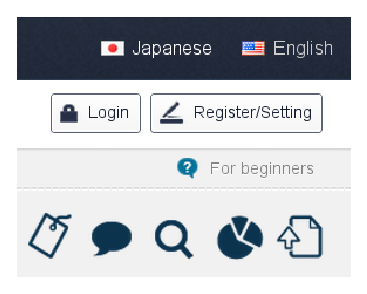
\includegraphics{aoj.eps}


自分の提出に対応する行(``Author''を見よ)の``Statusが ``\eindex{Accepted}''なら正答.


\paragraph{正答でなかった時}

様々な原因がありうるので,まずジャッジの応答がどれにあてはまるか,システムの使い方を誤解していないかなどを説明を読んで確認する.
Terms of use
(\url{https://onlinejudge.u-aizu.ac.jp/#/term_of_use}),
Judge's replies (\url{https://onlinejudge.u-aizu.ac.jp/#/judges_replies}),
チュートリアル (\url{http://judge.u-aizu.ac.jp/onlinejudge/AOJ_tutorial.pdf})
などの資料がある.

一般的に\textbf{プログラムが意図したとおりに動かないことは,誰でも(熟達者でも!)しばしばある}ことである.
組み上げたプログラムが動かなかったとしても,何から何までダメという事はなく,多くの場合はほんの少しの変更で解決することが多い.そこで,どの部分までは正しく動いているか,各部品ごとに動作確認をする方針が有効である.
コンピュータでのプログラミングは \textbf{copyやundoができる}ことが長所であるから,(料理で食材を無駄にしてがっかりするようなことは起こらない),臆せず色々試すと良い.

困った状況から復帰するノウハウも多少も存在する(付録 \ref{chapter:debug})
ので,徐々に身につけると有用であろう.
一方で,経験が少ない段階では,\cemph{15分以上悩まない}ことをお勧めする.
手掛かりなく悩んで時間を過ごすことは苦痛であるばかりでなく,初期の段階では学習効果もあまりないので,
指導者や先輩,友達に頼る,あるいは一旦保留して他の問題に取り組んで経験を積む方が良いだろう.
相談する場合は,「こう動くはずなのに(根拠はこう),実際にはこう動く」と問題を具体化して言葉にしてゆくと解決が早い.
なお,悩んで意味がある時間は,熟達に応じて2時間,2日間等伸びるだろう.

\section{入出力と問題の対応}

さっそく,AOJで1題回答してみよう.

\begin{psbox}{Rectangle}{AOJ}
たて a cm よこ b cm の長方形の面積と周の長さを求めるプログラムを作成し
て下さい。
  \aojid{ITP1_1_C}
\end{psbox}

以下の手順で取り組む:
\begin{enumerate}
\item 問題を把握する
\item 計算手順を検討する (今回は$a*b$と$a+b$を計算すれば良いことを把握する)
\item プログラムを書く.\jindex{エディタ}{えでぃた}(Emacs, mi などお好みで)で編集し,ファイルに保存する.
\item 手元のコンピュータで動作確認をする (必須)
\item AOJに提出して確認する
\end{enumerate}

\paragraph{解答例}: 以下に各言語の回答例と,\texttt{a=3}, \texttt{b=5}のケースに対する動作確認の方法を示す.

\begin{pybox}
a,b = map(int, input().split())
area = a*b
perimeter = 2*(a+b)
print("
\end{pybox}

\text{input()}で一行読み,
\texttt{split()}で空白区切りで分割し\footnote{この時,末尾の改行文字や(もしあれば)行頭や連続する空白文字も削除される.},\texttt{map(int, ...)}で分割
された各要素を整数に変換している。

上記の内容を\texttt{rectangle.py}などと保存したあと,\jindex{ターミナル}{たーみなる}上で実
行する.\texttt{\$}はプロンプトの略記であり,自身で入力する必要はない(つまり\texttt{python3}以降をタイプする)\footnote{詳しくはHWB15.2を参照 \url{https://hwb.ecc.u-tokyo.ac.jp/wp/information-2/cui/terminal/}}.また,\texttt{\#}とその右部分は補足説明であり,これも入力の必要はない.各行の入力終了時に,エンターキーを押すこと.以下,斜体はキーボードからの入力を示す.
\begin{terminal}
$ python3 rectangle.py
|3 5| # キーボードから入力する
15 16 # プログラムの出力の表示
\end{terminal}

\begin{cbox}
#include <iostream>
using namespace std;
int main() {
  int a,b;
  cin >> a >> b;
  // ここで area, perimeterを計算
  cout << area << ' ' << perimeter << "\textbackslash{}n";
}
\end{cbox}

上記のプログラムを,\texttt{rectangle.cc}などに保存する.続いてコンパイルして実行する.

「ターミナル」(MacOSXの場合)の動作例は以下の通り:
\begin{terminal}[emph={Wall,fsanitize}]
$ g++ -std=c++11 -Wall -fsanitize=undefined rectangle.cc # コンパイル
$ ./a.out # 実行
|3 5| # キーボードから入力する
15 16 # プログラムの出力の表示
\end{terminal}

\texttt{\#}とそれより右は,コメントであり,入力する必要はない.
\eindex{-std=c++11}は,C++11規格を有効にする\jindex{コンパイルオプション}{こんぱいるおぷしょん}である.
\eindex{-Wall}は様々な警告を有効にするオプションで,何か警告時にメッセージが出た場合
は解消することが望ましい.特に\cemph{プログラムの動作に疑問がある場合}は,\cemph{目立つ警告を解消してから質問}すること.
読み方が分からないメッセージが出た場合は,誰かと相談する.
\eindex{-fsanitize=undefined}は,実行時エラーを捕捉する機構を有効化する.動作確認の間はつけておくことが望ましい.詳しくは\ref{section:cpp-sanitize}章を参照.

\begin{warningbox}{C言語禁止}
  本資料を読み進める場合は,C言語では不十分で,C++の機能の一部を使う必要がある.必要な部分を少しづつ紹介するので,この時点で\texttt{iostream,cin,cout}などに慣れること.
\end{warningbox}

\begin{warningbox}{ブラウザ上のプログラミング禁止}
 簡単な問題はブラウザ上でコーディングすることもできるかもしれないが,今後扱う複雑な問題はそうではない.手元のPCでコンパイルして,様々なデータで実行できる環境を,この時点で用意しておくこと.
\end{warningbox}

\begin{cbox}
#include <cstdio>
int main() {
  int a,b;
  scanf("
  // ここで area, perimeterを計算
  printf("
}
\end{cbox}
この資料では,C言語使用者はC++に移行するよう推奨するが,C++を用い
る場合でも入出力はCの\texttt{scanf}, \texttt{printf}を用いて良い.

\begin{rbox}
a,b = gets.split(" ").map(&:to_i)
area = a*b
perimeter = 2*(a+b)
print sprintf("
\end{rbox}

上記の内容を\texttt{rectangle.rb}などと保存したあと,ターミナル上で実
行する
\begin{terminal}
$ ruby rectangle.rb
|3 5| # キーボードから入力する
15 16 # プログラムの出力
\end{terminal}

Javaの場合,オンラインジャッジシステムの制限で,常に\texttt{Main}というクラスに回答を書く必要がある.そのためには\texttt{Main.java}というファイル名で保存する必要があるので,問題毎にフォルダを作成し,そこで作業すること.
\begin{javabox}[emph={Main}]
import java.util.Scanner;
public class Main {
    public static void main(String[] args) {
	Scanner scanner = new Scanner(System.in);
	int a = scanner.nextInt(), b = scanner.nextInt();
	int area = a*b;
	int perimeter = 2*(a+b);
	System.out.println(area+" "+perimeter);
    }
}
\end{javabox}

\begin{terminal}
$ javac Main.java
$ java Main
|3 5| # キーボードから入力する
15 30 # プログラムの出力の表示
\end{terminal}


\section{実践上の注意事項}\label{section:commands}
\subsection{フォルダの保存}
各章では,サンプルや機能確認のために複数のコード片を扱う.
そこで,混乱を避けるため,\jindex{フォルダ}{ふぉるだ}を作って,テーマごとに別の名前をつけて
ファイルに保存すると良い.そして,それぞれを動作可能に保つ.
一方,お勧めしない方法は,一度作ったファイルを継ぎ足しながら,一つの巨大なファ
イルにすることである.そうしてしまうと,後から,2種類のコードを実行して差を
比べるようなことが難しくなる.

「ターミナル」(MacOSXの場合)の動作例は以下の通り:
\begin{terminal}
$ mkdir programming
# (フォルダ作成,最初の一回のみ)
$ mkdir programming/chapter1
# (各章毎に行う)
$ cd programming/chapter1
# (カレントディレクトリを変更.\$HOME/programming/chapter1/ 以下にソースコードを保存)
\end{terminal}

\subsection{標準入出力とリダイレクションによるファイルを用いたテスト}

この節では\cemph{データがあるだけ読み込む方法}と\cemph{ファイルを用いたテスト}の方法を紹介する.
この節の内容は,今ただちに身につける必要はないが,第2,3章に取り組む過程で身につけておくことが望ましい.

巨大な入出力を扱う場合は,キーボードから手で入力することは適切でない.
(手で入力すると,タイプミスのリスクがある.コピーペーストすると多少改善するが,データ量に上限があるり,また範囲選択のミスの余地が依然として残る.プログラムの正しさを検証する際には,他の不確定要因は100\%取り除き,プログラムそのものに集中することが望ましい.)

各問題では標準入出力を扱い,プログラムの正しさを入力に対する出力で判定
する.入力では,入力データがある限り読み込んで処理する場合も多い.
そこで,初めに例を挙げる.以下環境は基本的にMacOSXを想定するが,ubuntuやcygwin等でも動作すると思われる.

\begin{itembox}[l]{例題}
年を読み込んで,うるう年かどうかを判定し,日数を出力するプログラムを作る
\end{itembox}

(いい加減な)プログラム例 (C++): leap.cc

\begin{cbox}
// 4年に一度?
#include <iostream>
using namespace std;
int main() {
    int year;
    while (cin >> year) { // cinはboolに自動変換されるので入力が読める限りループ
      if (year 
        cout << 366 << endl;
      else
        cout << 365 << endl;
    }
}
\end{cbox}



\paragraph{コンパイル}

(前述の通り\$記号は,ターミナルへのコマンド入力を示す)

C++の場合:
\begin{terminal}
$ g++ -Wall leap.cc
\end{terminal}

Javaの場合:
\begin{terminal}
$ javac Main.java
\end{terminal}

\paragraph{実行例}
斜体はキーボードからの入力を示す.終了はCtrlキーを押しながら c
または dをタイプする.この操作を\^{}Cや\^{}Dと表記する.

\begin{terminal}
$ ./a.out
|2004|
366
|1999|
365
|1900|
366
|2000|
366
|^D|
\end{terminal}

\paragraph{ファイルを用いたテスト}
実行するたびに毎回キーボードをタイプするのは煩雑であるから,自動化した
い.
そこで,リダイレクションとファイルを用いたテストを解説する.
早い段階で身につけることが望ましい.

正しい入出力例をエディタで作成し,\texttt{cat}コマンドで中身を確認する:
\begin{terminal}
$ cat years.input
2004
1999
1900
2000
$ cat years.output
366
365
365
366
\end{terminal}

\jindex{リダイレクション}{りだいれくしょん}を使った実行(キーボード入力の代わりにファイルから読み込む):
\begin{terminal}
$ ./a.out < years.input
366
365
366
366
\end{terminal}

実行結果をファイルに保存(画面に表示する代わりにファイルに書き込む):
\begin{terminal}
$ ./a.out < years.input > test-output
$ cat test-output
366
365
366
366
\end{terminal}

\eindex{diff}を用いた自動的な比較:
\begin{terminal}
$ diff -u test-output years.output
--- years.output        Fri Oct 14 10:53:52 2005
+++ test-output Fri Oct 14 10:53:56 2005
@@ -1,4 +1,4 @@
 366
 365
-365
+366
 366
\end{terminal}
4行目あたりが違うことを教えてくれる


\begin{itembox}[l]{資料:}
\begin{itemize}
\item HWB 15 コマンド\\
  \url{http://hwb.ecc.u-tokyo.ac.jp/wp/information-2/cui/}
\item HWB 14.4 コマンドを使ったファイル操作\\
 \url{http://hwb.ecc.u-tokyo.ac.jp/wp/information-2/filesystem/cui-fs/}
\end{itemize}
\end{itembox}

\subsection{ジャッジデータのダウンロードと手元での実行}\label{run-judge-data}
プログラムを提出した際に,Acceptedではなく \eindex{Wrong Answer}や\eindex{Time Limit Exceeded},
\eindex{Rutime Error}などとなる場合がある.

仮に今\texttt{ITP1\_4\_D}という問題を解いていて,Wrong Answerになったとする.

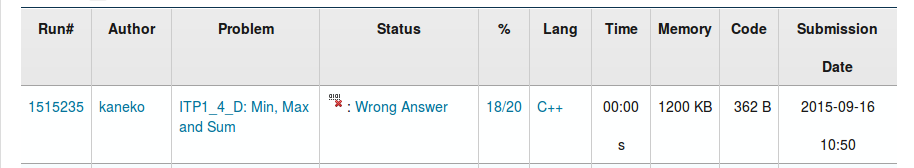
\includegraphics[width=.9\linewidth]{2.png}

中央付近の18/20という数字は,テストケースの18番目まで正答し,19個目で失敗したという意味である.その部分がハイパーリンクになっているのでクリックすると,詳細が分かる.

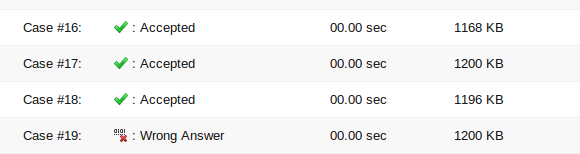
\includegraphics[width=.7\linewidth]{3.png}

さらに \texttt{Case \#19:}の行をクリックすると,実際のデータを見ることができる(問題による).

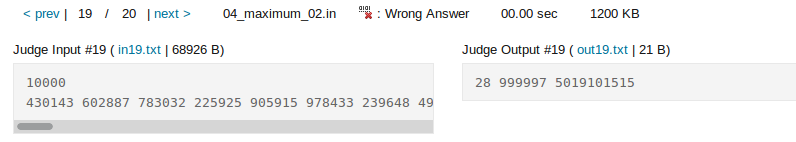
\includegraphics[width=.9\linewidth]{4.png}

このデータを手元で試してみよう.
データは,コピーペーストするには大きすぎるので,まず\texttt{in19.txt}の部分をクリックしてダウン
ロードする.
環境やブラウザによるが\texttt{ITP1\_4\_D\_in19.txt}という名前でダウンロー
ドフォルダなどに保存されたとする.適宜,リダイレクションによって実行
する.

\begin{terminal}
$ ./a.out < ~/Downloads/ITP1_4_D_in19.txt 
28 999997 724134219  
\end{terminal}

また,今回はプログラムの出力とJudge Outputとの間に差があることは一目でわかるが,一般に5019101515のような桁数の数字を目で比較す
るのは困難であるから(1文字異なっていても気づかない),同様にダウンロー
ドして\texttt{diff}コマンドにより比較するのが良い.

実行結果をファイルに保存(画面に表示する代わりにファイルに書き込む):
\begin{terminal}
$ ./a.out < sample-input.txt > my-output.txt
$ cat my-output.txt
1 17 37
\end{terminal}

2つのファイル比較:
\begin{terminal}
$ diff -u sample-output.txt my-output.txt
\end{terminal}
(差分がある場合のみ,出力がある)
 % Commented out: Included file

\part{Introductory Course}

%\chapter{入出力と配列・シミュレーション}\label{chapter:io}
\begin{itembox}[l]{概要}
様々な解法につながる基本として,入力データを逐一調べる問題から始めて,配列と周辺の基本操作をとりあげる.
また,プログラムを一度に作成するのではなく,部品ごとに作ってテストするスタイルを身につける.
さらに,データの量に応じて,適切なアルゴリズムが必要になることを経験する.
\end{itembox}


\section{最大値,最小値}

\begin{psbox}{ICPC Score Totalizer Software}{国内予選2007}
入力として与えられる数値列から最大値と最小値を除いた平均値を求めよ.

入力はそれぞれが競技者の演技ひとつに対応するいくつかのデータセットからなる. 入力のデータセット数は20以下である.
データセットの最初の行はある演技の採点に当たった\uline{審判の数 n} ($3 \le n \le 100$) である.引き続く n 行には各審判のつけた \uline{点数 s} ($0 \le s \le 1000$) がひとつずつ入っている. n も各 sも整数である.入力中にはこれらの数を表すための数字以外の文字はない.\sout{審判名は秘匿されている.}
入力の終わりはゼロひとつの行で示される. 
  
\aojid{1147}
\end{psbox}


``Sample Input''を順に解釈すると,以下のように4つのデータセットからなることが分かる.
\begin{itemize}
\item (N=) 3 (S=) 1000 342 0
\item (N=) 5 (S=) 2 2 9 11 932 
\item (N=) 5 (S=) 300 1000 0 200 400
\item (N=) 8 (S=) 353 242 402 274 283 132 402 523
\item 0 (入力の終わり)
\end{itemize}

\begin{alltt}
#--------
3 # データは3つ, N=3
1000 # 最大値
342
0 # 最小値
#--------
5 # データは5つ, N=5
2 # 最小値
2
9
11
932 # 最大値
#--------
5 # データは5つ
300
1000 # 最大値
0 # 最小値
200
400
#--------
8 # データは8つ
353
242
402
274
283
132
402
523
#--------
0 # これでおしまい
\end{alltt}


同様に``Sample Ouput''を解釈すると,上記の各データセットに対して一つ数
値が出力されていることが分かる.
\begin{itemize}
\item 342 (そのまま)
\item 7 (2, 9, 11の平均)
\item 300 (300, 200, 400の平均)
\item 326 (...の平均)
\end{itemize}

\subsection{プログラム作成}

以下に,審判の得点の合計を計算するプログラムと最大得点を計算するプログラムを示す.(問題が求めるもの
は合計や最大値ではないので,これらは問題への直接の回答ではない).
必要ならばこれらのプログラムを参考に,問題への回答を作成せよ.

\begin{cbox}[emphstyle={[2]\graytext},emph={[2]iostream,using,namespace,std,cin,cout,endl}]
#include <iostream>
using namespace std;
int N, S;
int main() {
    while (cin >> N && N>0) {
        int sum = 0;
        for (int i=0; i<N; ++i) {
            cin >> S;
            sum += S; // std::accumulateを使っても良い
        }
        cout << sum << endl;
    }
}
\end{cbox}

\begin{cbox}[emphstyle={[2]\graytext},emph={[2]iostream,using,namespace,std,cin,cout,endl}]
// (一部略)
    while (cin >> N && N>0) {
        int largest = 0;
        for (int i=0; i<N; ++i) { // std::max\_elementを使っても良い
            cin >> S;
            if (largest < S) largest = S;
        }
        cout << largest << endl;
    }
\end{cbox}
C言語からC++に移行する場合は,(基本は共通なので)さしあたり\cplusplus{網掛け}部分を覚えて使えるようになると良い.
コンパイルの仕方などは\ref{section:commands}節を参照.

\begin{warningbox}{C言語禁止}
  本資料を読み進める場合は,C言語では不十分で,C++の機能の一部を使う必要がある.必要な部分を少しづつ紹介するので,この時点で\texttt{iostream,cin,cout}などに慣れること.
\end{warningbox}

\begin{tipsbox}{関数を使おう}
  \texttt{max,min,sum}などは関数を使っても良い.
\end{tipsbox}

\begin{pybox}
while True:
    N = int(input())
    if N == 0:
        break
    S = []
    for i in range(N):
        S.append(int(input()))
    print(sum(S))
    print(max(S))
\end{pybox}
なお,Python3で整数除算を行うには\texttt{/}に代えて\texttt{//}という演算子を用いる.


\subsection{動作テスト}

\subsubsection{サンプル入力を用いたテスト}

問題文中の``Sample Input''に対する出力が合うことを確認してみよう.

\subsubsection{審判データを用いたテスト}
この問題は審判が用いた秘密の入出力が公開されている.これを利用し
て, プログラムの誤りの有無をさらに手元で試験することができる.
(プログラムが``Sample Input'' には正しく振舞うが,他のデータには誤ることを発見できるかもしれない)
\begin{itemize}
\item 入力 \url{http://www.logos.ic.i.u-tokyo.ac.jp/icpc2007/jp/domestic/datasets/A/A1}
\item 出力 \url{http://www.logos.ic.i.u-tokyo.ac.jp/icpc2007/jp/domestic/datasets/A/A1.ans}
\end{itemize}

出力の一致を確認するには,\texttt{diff}コマンドを用いる.
実行方法などは\ref{section:commands}節を参照.

\begin{terminal}
$ python3 icpc.py < A1 > my-out.txt
$ diff -u my-out.txt A1.ans  
\end{terminal}

\begin{terminal}
$ ./a.out < A1 > my-out.txt
$ diff -u my-out.txt A1.ans  
\end{terminal}

\begin{warningbox}{後回し禁止}
  この時点で(次の章に進む前に)リダイレクションと\texttt{diff}の操作を覚えること.
\end{warningbox}


\section{計算時間の見積と試行回数}

コンピュータが得意な解法は全部を力づくで試すことである.実際に多くの問題をそれで解くことが出来る.
コンピュータが得意な解法は全ての可能性を力づくで試すことである.実際に多くの問
題をそれで解くことが出来る.
全ての可能性を列挙するには,for文を用いたり,再帰を用いたりする.

\begin{pbox}{Tax Rate Changed}{国内予選2014}
2つの商品の消費税率変更前の税込合計価格を元に, 新消費税率での税込合計
価格が最大いくらになるかを計算するプログラムを作って欲しい. 1円未満切り捨て等の細かい条件は問題文を参照のこと. 

制約(抜粋): $10 < s < 1000$, 商品の税抜価格は$1$円から$s-1$円のすべてを考慮に入れる

Time Limit : 8 sec, Memory Limit : 65536 KB

\aojid{1192}
\end{pbox}

 (1) 2つの商品の価格の候補の組み合わせを全通り試す.(2) 候補が,変更前
の税率で合計価格になっているかを調べる.そうでなければ捨てる (3) 変更
後の税率での合計価格を計算する.最大値なら記憶する.
という方針で作ってみよう.

仮に税込みの価格を計算する\texttt{tax(rate, price\_without\_tax)}という関数があっ
たとすると,次のような構造になるだろう.問題文では小文字の$s$を使って
いるが,本資料のプログラムでは(i, j, kなどの変数と区別して問題文由来である目印に)大文字で表記する.
\begin{cbox}
  int maximum = 0;
  for (int i=1; i<S; ++i)
    for (int j=i; j<S; ++j) 
      if (tax(X,i)+tax(X,j) == S) // (*)
        maximum = max(maximum, tax(Y,i)+tax(Y,j));
\end{cbox}
なおこの例題はさらに,繰り返し回数を減らすための工夫を検討することもで
きるが,C++なら今回は必須ではない.
Pythonの場合は,多少の工夫が必要である.下記のコードでは,ある組$(a_0,b_0)$の税込価格が$S$を越えたら,$b>b_0$での組$(a_0,b)$の税込価格も$S$を必ず超えるので,検討不要であるという性質を利用した.

\begin{warningbox}{関数必須 (横着禁止)}
  必ず関数 \texttt{tax}を作成すること.徐々に複雑なプログラムを扱う際に,関数の作成能力は重要となる.この時点で身につける.
\end{warningbox}

\begin{pybox}[emph={break}]
def tax(p,x):
    return p*(100+x) // 100     # 整数除算
def solve(X,Y,S):
    for a in range(1,S):
        for b in range(1,S):
            sum = tax(a,X)+tax(b,X)
            if sum == S:
                # 新税でのtax(a,Y)+tax(b,Y) について検討
            if sum > S:
                break           # b増加ならばsum増加のため
    return best
while True:
    X,Y,S = map(int, input().strip().split(' '))
    if X == 0:
        break
    print(solve(X,Y,S))
\end{pybox}

\begin{debugbox}{TLE (Time limit exceeded)}
  Pythonの場合はC++よりも実行速度が遅くなるため,C++と同じ方針ではACを
  得られない場合がある.例えば,上記のサンプルコードでは9,10行目に高速化のための工夫を施している.
\end{debugbox}

\begin{warningbox}{税込み v.s. 税抜き}
  本資料では,税抜価格と税率から税込価格を求める関数を作成した.向きを反対にして,税込み価格から税抜価格を求めるアプローチはどうだろうか.実はそちら向きは罠が多数あるのでお勧めしない(興味がある場合はお勧めの方法でAC後に理由を考えてみよう).
\end{warningbox}

\paragraph{複数データセットの入力}
この問題ではデータセットが複数与えられうる.すなわち,データが与えられ
る間はそれを読み込んで解を出力し,データが終了したらプログラムを終了さ
せる必要がある.「入力の終わりは,空白で区切られた3つのゼロからなる行
によって示される. 」という条件と通常のデータセットでは\texttt{X}が正であることを活用し,以下の構造でプログラムを書くことを勧める.

\begin{cbox}
#include <iostream>
using namespace std;
int X, Y, S;
int solve() {
  ... // X,Y,Sについて,最大値を計算
}
int main() {
    while (cin >> X >> Y >> S && X>0) {
	cout << solve() << endl;
    }
}  
\end{cbox}

\texttt{while}文の条件の\texttt{cin >> X >> Y >> S}の部分は\text{cin}への参照を
返し,\texttt{bool}にキャストされた際に,\texttt{cin}が正常状態かどう
か,すなわち\texttt{X, Y, S}を正常に読み込めたかどうかを返す.入力ファイルが間違っていた(よくある場合は,タイプミスまたは違う問題の入力を与えた)場合はここが\texttt{false}になって終了する.読み込めた場合に,\texttt{X, Y, S}は処理すべきデータセットの\texttt{X, Y, S}を読んだ場合と,入力終了の目印の空白で区切られた3つのゼロを読んだ場合の両方がある.前者の場合は正の整数であるはずなので,0かどうかをテストして判別する.

\paragraph{AOJへの提出}

上記の方針でプログラムを作成し,AOJでacceptされることを確認せよ.

もしacceptが得られなかった場合は手元での検証が可能である.まず,入力
(\url{http://icpc.iisf.or.jp/past-icpc/domestic2014/qualify14_ans/A1})
と正答
(\url{http://icpc.iisf.or.jp/past-icpc/domestic2014/qualify14_ans/A1.ans})
をダウンロードしておく.
\begin{terminal}
  $ ./a.out < A1 > my-output.txt
  $ diff -u A1.ans my-output.txt 
\end{terminal}
差があれば行数が表示される.

\paragraph{計算量の簡単な検討 (estimation of the number of trials)}
多くのコンテストの問題では実行時間に制限がついているので,実行
時間を見積もり間に合う解法を考案することが必要な場合もある.またコンテ
ストを離れて実用に用いるプログラムでも,何らかの実行速度に関する要請が
ある場合が多い.プログラムを書き終えてから速度に問題があることが分かる
と,書き直しが困難な場合もあるので,プログラムを書く*前*に何らかの見通
しを得ておくことが望ましい.

現実の計算機は複雑な装置であるから,正確な実行時間の予想は簡単ではない.よって単純なモデルに基づく目安を考える.
たとえば,プログラムを実行する過程で,加減乗除のような基本演算が何回行
われるかを数える.このモデルでは加算と除算では速度が異なりうるとか,同時に
二つの命令を実行される場合があるなどの,細かい点は無視している.目安で
あるので現実との対応関係は別に議論が必要だが,役に立つ場面も多い.


上記のプログラムで4行目(*)が最大何回実行されるか,考察しよう(厳密に求めなくて良い).
回数を($S$に依存するので),$f(S)$と表すとする.2行目の\texttt{for}ループ
が$S$回,3行目の\texttt{for}ループが最大$S$回繰り返すので,$f(S) \le
S^2 \le 1\,000^2=10^6$である.

\begin{table}[h]
  \centering
  \caption{\cemphp{C++}で,1秒間で実行可能な演算回数の目安 (\cite{book:pcc}を改変して転載)}
  \label{table:empirical-estimation}
  \begin{tabular}{rl}\hline
    $1\,000\,000$  &余裕を持って可能\\
    $10\,000\,000$ &たぶん可能\\
    $100\,000\,000$&とてもシンプルな演算なら可能\\\hline
  \end{tabular}
\end{table}

この回数($10^6$)を表\ref{table:empirical-estimation}に当てはめると,(tax関数が効率的に実装されていることを前提に)余裕を持っ
て,1秒間で実行可能と分かる.\footnote{注: この見積もりは1つのデータセットについてのものである.一方,問題全体では「入力は複数のデータセットからなる」ものを8秒間で回答する必要があるため,計算時間はデータセット数の上限を考慮して見積もる必要がある.データセットの数について記述がない場合は,厳密には問題の不備であるが,10個程度と考えて良い.}
表の数値は,実行環境に合わせて経験的に測定する必要がある.
目安として,最近の多くのコンピュータのCPUは1GHz ($=10^{9}$)程度で動作しているので,CPUが100サイクル以内に実行できる演算なら,1秒間に$10^6$回実行可能と期待できる.

本資料の範囲では,この表を信じて問題ない場合がほとんどであるが,
正確な予測のためには,キャリブレーションを行う.すなわち,作成した解法が入力に対応する数値$N$に関しておよそ何回の基本演算を行う
かを見積もったら,いくつかの$N$に対応する入力で実験し,実際の計算秒数
との対応を取る.たとえばメモリ参照やnew/deleteは,算術演算よりそれぞれ10倍,100倍以上に遅い場合がある.また,C, C++以外の言語では,実行により時間がかかることも多い.問題ごとの秒数制限と,オンラインジャッジのハードウェアを考慮して検討する.

\begin{tipsbox}{Pythonの場合はC++よりも実行速度が遅くなる}
  問題によるが20-200倍余裕
  をもって見積もると良い.オンラインジャッジで時間制限は
  Pythonに適切とは限らないので,ジャッジデータをダウンロードして正答を確認できればそれでも良い.
\end{tipsbox}


\begin{pbox}{Space Coconut Grab}{模擬国内予選2007}
宇宙ヤシガニの出現場所を探す.エネルギーEが観測されたとして,
出現場所の候補は,$x+y^2+z^3=E$を満たす整数座標(x,y,z)で,さらにx+y+zの
値が最小の場所に限られるという.x+y+zの最小値を求めよ.
(x,y,zは非負の整数,Eは正の整数で1,000,000以下,宇宙ヤシガニは,宇宙最大とされる甲殻類であり,成長後の体長は 400 メートル以上,足を広げれば 1,000 メートル以上)

\aojid{2012}
\end{pbox}

まず,全部試して間に合うかを考える.
(間に合うならそれが一番実装が簡単なプログラムである)

変数x,y,zの動く範囲を考えると,それぞれx:[0,E], y:[0,$\sqrt{E}$],
z:[0,${}^3\sqrt{E}$]である.それら(x,y,z)の組み合わせは,Eの最大値は
1,000,000$=10^6$であるから,最大$10^6 \cdot 10^3 \cdot 10^2=10^{11}$で
ある.
制限時間が8秒であることを加味しても,この方針では間に合いそうにない.

減らす指針として,全ての(x,y,z)の組み合わせを考える必要はなく,
$x+y^2+z^3=E$を満たす範囲だけで良いことを用いる.たとえば,xとyを決める
と,Eからzは計算できる(zが整数とならない場合は無視して良い).この方針で
調べる種類は,(x,y)の組み合わせの種類である,$10^6 \cdot 10^3$となる.
この値はまだ大きいが,先ほどと比べると1/100に削減できている.上記と同様
に,xとzを決めてyを求める,z,yを決めてxを求めることもできる.それらの方
針の場合に,調べる組み合わせの種類を求めよ.一番少ないものが間に合う範
囲であることを確認し,実際に実装してAOJに提出して確かめる.

\begin{debugbox}{Python--TLE}
残念ながら上記の方針ではPythonでは時間制限を超過(TLE)する.対策として
は,2重ループを避けて\texttt{z}に関する1重ループのみにすれば良い.
単調性から\texttt{y}に関するループを省くことが出来る.
\begin{pybox}
import math
# ...(中略)...
y = int(math.floor(math.sqrt(E-z**3)+1e-7))
\end{pybox}
\end{debugbox}

\section{練習問題}
\begin{pbox}{Square Route}{模擬国内予選2007}
縦横1500本程度の道路がある街で,正方形の数を数えてほしい.

\aojid{2015}
\end{pbox}

注: 全ての4点を列挙して正方形になっているかどうかを試すと間に合わないので,工夫した方法が必要である.正方形を一つづつ数えると数が多すぎるので,一定の性質を持つ正方形をまとめて数えるような方法が必要となる.

ヒント: 後の章で扱う標準データ構造を活用する方法と,正方形の初等的な性質を利用する方法がある(\textcolor{white}{対角線を延長した直線を共通に持つ正方形}について考えてみよう).


\chapter{整列と貪欲法}\label{chapter:greedy}

\begin{itembox}[l]{概要}
ある基準に従ってデータを並べ替えることを整列(sort)という.
ほとんどの言語の標準ライブラリでは,整列の方法が提供されているので,ま
ずはそれの使い方を習得しよう.この資料では整列された結果
を得られれば良いという立場をとるが,整列の手法そのものに興味がある場合は,たとえ
ば~\pcaojbook[pp.~51--(3章)]を参照されたい.

データの整列は,問題解決の道具として活躍する場合もある.それらには,最適化問題や配置問題など,整列とは関係がない見た目の問題も含まれる.
\end{itembox}

\section{さまざまな整列}

\subsection{数値の整列}\label{section:sort}

C++とRubyでは,標準関数として\texttt{sort}や\texttt{sort!}が用意されている.
\begin{cbox}[emph={algorithm,sort}]
#include <algorithm>
#include <iostream>
using namespace std;
int A[5] = {3,5,1,2,4};
int main() {
   sort(A,A+5); // 半開区間[l,r)で指定する.sort(\&A[0], \&A[5])と同じ意味
   ... // coutにAを出力してみよう
}
\end{cbox}
配列を整列させる範囲を指定するには,\texttt{\&A[0]}のように配列の要素を指すポインタを用いる.一次元配列の場合に単に\texttt{A}と書けば,先頭要素を指すポインタに自動的に変換される.
配列でなく\texttt{vector}や\texttt{array}の範囲を指定するには,
\texttt{A.begin(),A.end()}という表記を用いる.この\texttt{begin}や\texttt{end}はポインタを一般化したイテレータを返す関数で,名前の通りの場所を指し示す.他に\texttt{A.begin()+2,A.begin()+5}のように一部の区間を指定することもできる.さらにC++11以降では\texttt{begin(A)}とすることで配列もvectorも共通に扱うことができる.

\begin{pybox}[emph=sort]
a = [3,5,1,2,4]
a.sort()
a
# [1, 2, 3, 4, 5]  
\end{pybox}


\begin{psbox}{Sort II}{AOJ}
 与えられたn個の数字を昇順に並び替えて出力するプログラムを作成せよ. 

\aojid{10029}
\end{psbox}

回答例:
\begin{cbox}
int N, A[1000000+10];
int main() {
    cin >> N;
    for (int i=0; i<N; ++i) cin >> A[i]; // Aの入力
    ... // Aをソートする
    for (int i=0; i<N; ++i) cout << (i?" ":"") << A[i]; // Aの出力
    cout << endl;
}
\end{cbox}

出力部分の\texttt{(i?" ":"")}は,要素の間にのみ空白文字を入れるための微調整(先頭\texttt{i==0}には空白を入れない).

\subsection{文字列の整列}

\begin{psbox}{Finding Minimum String}{AOJ}
N個の小文字のアルファベットのみからなる文字列の,辞書順で先頭の文字列
を求める.
問題文中に記述がないがNは1000を越えない.

\aojid{10021}
\end{psbox}

補足: 辞書式順序は,大文字小文字が混ざる場合はC++の\texttt{std::string}の比較演算子の比較順序とは異なる.(が,今回は小文字のみなのでその心配はない)

\begin{cbox}
#include <algorithm> // sortのため
#include <string> // string (文字列)のため
#include <iostream>
using namespace std;
string A[1000];
int N;
int main() {
    cin >> N;
    if (N > 1000) abort();
    for (int i=0; i<N; ++i) cin >> A[i];
    ... // 整数の時と同様にAを整列(sort)する
    cout << A[0] << endl;
}
\end{cbox}

\subsection{ペアと整列}\label{section:sort-pairs}
\subsubsection{ペア}
ペア(組み)の表現を導入する.$\langle$開始時刻,終了時刻$\rangle$や$\langle$身長,体重$\rangle$,$\langle$学籍番号,点数$\rangle$など,現実世界の情報にはペアとして表現することが自然なものも多い.

\begin{cbox}
#include <utility> // pairのため
#include <iostream>
using namespace std;
int main() {
  pair<int,int> a(2,4); // 整数のペア
  cout << a.first << ' ' << a.second << endl; // 2 4と表示

  a.first = 3;
  a.second = 5;
  cout << a.first << ' ' << a.second << endl; // 3 5と表示

  a = make_pair(10, -30);
  cout << a.first << ' ' << a.second << endl; // 10 -30と表示

  pair<double,char> b; // 小数と文字のペア
  b.first = 0.5;
  b.second = 'X';
  cout << b.first << ' ' << b.second << endl; // 0.5 Xと表示
}
\end{cbox}

Pythonやruby の場合は列(配列やリスト)を手軽に使えるので,(取り立ててpairを区別せず)列を使う.



\subsubsection{ペアの配列と整列}
続いて,ペアの配列を扱う.たとえば,一人の身長と体重をペアで表現する時に,複数の人の身長と体重のデータはペアの配列と対応づけることができる.
前回,整数の配列を整列(\texttt{sort})したように,ペアの配列も整列することができる.
標準では,第一要素が異なれば第一要素で順序が決まり,第一要素が同じ時には第二要素が比較される.

\begin{cbox}
#include <utility> // pairのため
#include <algorithm> // sortのため
#include <iostream>
using namespace std;
int main() {
  pair<int,int> a[3]; // 整数のペア
  a[0] = make_pair(170,60);
  a[1] = make_pair(180,90);
  a[2] = make_pair(170,65);

  for (int i=0; i<3; ++i) // a[0]からa[2]まで表示
    cout << a[i].first << ' ' << a[i].second << endl;
  // 170 60
  // 180 90
  // 170 65 と表示されるはず

  sort(a, a+3); // a[0]からa[2]まで整列

  for (int i=0; i<3; ++i) // a[0]からa[2]まで表示
    cout << a[i].first << ' ' << a[i].second << endl;
  // 170 60
  // 170 65
  // 180 90 と表示されるはず
}
\end{cbox}

\begin{pybox}
a = [[3,5],[2,9],[3,6]]
print(a) # [[3, 5], [2, 9], [3, 6]]
a.sort()
print(a) # [[2, 9], [3, 5], [3, 6]]
\end{pybox}

\subsubsection{3つ以上の組}
C++11では,3つ以上の組を表す\texttt{tuple}型が用意されている.\footnote{\url{http://en.cppreference.com/w/cpp/utility/tuple}}
それより前のC++では\texttt{pair<int,pair<int,int> >}などと\texttt{pair}を重ねて用いていたところが,簡潔に書けるようになった.

\begin{c11box}[emph={tuple}]
#include <tuple>
#include <iostream>
#include <algorithm>
using namespace std;
int main() {
  tuple<int,int,int> a = {3,1,4};
  cout << get<0>(a) << "\n";	// 3
  cout << get<1>(a) << "\n";	// 1
  cout << get<2>(a) << "\n";	// 4

  tuple<int,int,int> array[] = {{3,1,4}, {1,5,9}, {2,6,5}};
  sort(array, array+3);
  
  tuple<int,int,int> t = array[0];
  cout << get<0>(t) << "\n";	// 1
  cout << get<1>(t) << "\n";	// 5
  cout << get<2>(t) << "\n";	// 9
}
\end{c11box}


\subsection{大きい順に整列}
標準の\texttt{sort}関数は小さい順に並べ替える.大きい順に並べ替えるに
はどのようにすれば良いだろうか?
\begin{enumerate}
\item 小さい順に並べ替えた後に,並び順を逆転させる (当面これで十分)
\begin{cbox}
int A[5] = {3,5,1,2,4};
int main() {
   sort(A,A+5);
   // C++11なら sort(begin(A),end(A));
   reverse(A,A+5); // 与えられた範囲を逆順に並び替え
   ...  // coutにAを出力してみよう
}
\end{cbox}
\begin{pybox}
a = [3,5,1,2,4]
a.sort()
a.reverse() # aを逆順に並び替え
\end{pybox}
\item \texttt{reverse\_iterator}を使う
\begin{c14box}[emph={rbegin,rend}]
  sort(rbegin(A),rend(A));
\end{c14box}
\begin{pybox}
a.sort(reverse=True) 
\end{pybox}
\item 比較関数を渡す (汎用的)
\begin{c11box}
int A[5] = {3,5,1,2,4};
int main() {
   sort(begin(A),end(A),[](int p, int q){ return p > q; });
   ...  // coutにA[i]を出力してみよう
}
\end{c11box}
文法の説明は省略するが\texttt{[](int p, int q)\{ return p > q; \}}の部分が2つの整数の並び順を判定する匿名関数である.
\begin{pybox}
a.sort(key=lambda e: -e)  
\end{pybox}
\end{enumerate}

\section{貪欲法}

\subsection{良い順に使う}
\begin{pbox}{カントリーロード}{UTPC 2008}
カントリーロードと呼ばれるまっすぐな道に沿って, 家がまばら
に建っている. 指定された数までの発電機と電線を使って全ての家に給電したい. 
家に電気が供給されるにはどれかの発電機に電線を介してつな
がっていなければならず, 電線には長さに比例するコストが発生する. できるだけ電線の長さの総計が短くなるような発電機 お
よび電線の配置を求める.

\aojid{2104}
\end{pbox}

ヒント: 発電機が一つなら,端から端まで全ての家を電線でつなぐ必要がある.
発電機が2つなら,端から端まで全ての家を電線でつないだ状態から,家と家
の間の一箇所に電線を引かずに節約することができる.つまり,一番長い一箇所を節約するのが得.
発電機が3つなら,端から端まで全ての家を電線でつないだ状態から,家と家
の間で一番長い部分と二番目に長い部分には電線を引かずに節約することができる....

\begin{tipsbox}{方針の確認}
プログラムを書く前にSample Inputを手で解いてみよう
\end{tipsbox}


回答例
\begin{cbox}
int T, N, K, X[100000+10], A[100000+10];
int main() {
    cin >> T; // データセットの数を読み込む
    for (int t=0; t<T; ++t) {
        ... // 家と発電機の数を読み込む
        for (int i=0; i<N; ++i) cin >> X[i]; // 家の位置を入力
        for (int i=0; i+1<N; ++i) A[i] = X[i+1]-X[i]; // 家と家の間
        ... // 配列Aを整列する
        ... // 配列Aの先頭max(0,N-1-(K-1))個の和を出力する
    }
}
\end{cbox}

Python3の入力例: 与えられた1行を配列として読み込む場合は\texttt{list(...)}で変換する
\begin{pybox}
N,K = map(int,input().strip().split(' '))
X = list(map(int,input().strip().split(' ')) # リストへの変換を明示
\end{pybox}

\begin{debugbox}{よくある考え漏れ}
発電機\textcolor{white}{の個数が家の数を越えて増えても}節約できる区間は増えない (ヒントが白い文字で書かれているので,読みたくなったらコピーペーストなどで読むと良い).
\end{debugbox}

このような解法が貪欲法(greedy)と呼ばれる意味は,節約する区間の「組み合わせ」を
考えることなく,(長さ順に並べた)単独の区間を順に一つづつ見て閾値を越えるまで節約することを貪欲に決める点である.

\begin{pbox}{Stripies}{Northeastern Europe 2001}
質量が$m_1,m_2$である2体合体すると,$2\sqrt{m_1\cdot m_2}$となる種族がある.
初期状態を与えられるので,全てが合体した時の最小の質量を求めよ.

\url{http://poj.org/problem?id=1862}
\end{pbox}

小数点以下3桁を出力するには\texttt{printf("\%.3f\textbackslash{}n", ret);}を用いる.

\begin{pbox}{Princess's Marriage}{模擬国内予選2008}
護衛を上手に雇って,道中に襲われる人数の期待値を最小化する.
護衛は1単位距離あたり1の金額で,予算がある限り,自由に雇える.

入力は,区間の数N, 予算Mに続いて,距離と1単位距離あたりの襲撃回数の期
待値のペア$\langle$D,P$\rangle$がN個.  


\aojid{2019}
\end{pbox}

考え方:
せっかく護衛を雇うなら,もっとも危険な区間を守ってもらうのが良い.
一番危険な道を選び,予算がある限りそこに護衛を雇う.予算の残額で道の区間全てをカバーできない場合は,安全になる区間と,危険なままの区間に道が分かれる.予算が残っている限り,2番目に危険な道,3番目に危険な道の順に同様に繰り返す.残った危険な区間について,期待値の和が答えとなる.
この計算課程では,$\langle$危険度,長さ$\rangle$のペアで道を表現し,危険な順に整列しておくと便利である.  (ここで危険度は,距離1移動する間に襲われる回数の期待値を表す)

回答例 (入力と整列):
\begin{cbox}
int N, M;
pair<int,int> PD[10010];
int main() {
  while (cin >> N >> M && N) {
    int d, p;
    for (int i=0; i<N; ++i) {
      cin >> d >> p;
      PD[i] = make_pair(p, d);
      // PD[i].first は道iの危険度
      // PD[i].second は道iの長さ
    }
    ... // PDを大きい順に整列しよう
    // 整列がうまく行ったか,PDを表示してみよう
    // うまく整列できたら,次は答えを計算しよう
  }
}
\end{cbox}

回答例 (答えの計算):
\begin{cbox}
    int S = 0;
    for (int i=0; i<N; ++i)
      S += 道[i]の危険度 * 道[i]の長さ;
    // 予算0の時の答えが,現在のSの値
    for (int i=0; i<N; ++i) {
      if (M <= 0) break;
      int guarded = Mと道[i]の長さの小さい方; // 雇う区間
      S -= 道[i]の危険度 * guarded;
      M -= guarded;
    }
    S が答え
\end{cbox}

\begin{itemize}
\item 予算が0の場合は,答えとして必要な ``刺客に襲われる回数の期待値''である $S$は,各道$i$について$S=\sum_i P_i\cdot{}D_i$となる.
\item 予算がMの場合,$S$から護衛を雇えた区間だけ期待値を減らす.例えば
  道$j$の区間全部で護衛を雇うなら $P_j\cdot{}D_j$だけ$S$を減らすことができる.もし残り予算$m$が道の長さ$D_j$より小さく道の一部だけしか護衛を雇えないなら$S$から減らせるのは$P_j\cdot{}m$だけである.
\end{itemize}

\subsection{区間スケジューリング}

「アルゴリズムデザイン」\cite{book:algorithmdesign}の4.1章(pp.~104--108)を参照.

\paragraph{問題概要}
一つの共有資源(体育館,駐車場など)と多数の利用申請(開始時刻と終了時刻
のペア)があったとする.使用時間が衝突しないように,利用申請の部分集合
を選ぶ.最大いくつの申請を採用できるか?

\centerline{\begin{tikzpicture}
\draw (3,3.5) -- node[above]{$$} (5,3.5) node[right]{$0$};
\draw (1,3) -- node[above]{$$} (3.5,3) node[right]{$1$};
\draw (6,2.5) -- node[above]{$$} (7,2.5) node[right]{$2$};
\draw (2,2) -- node[above]{$$} (4.5,2) node[right]{$3$};
\draw (1.5,1.5) -- node[above]{$$} (2.5,1.5) node[right]{$4$};
\draw (4,1) -- node[above]{$$} (7.5,1) node[right]{$5$};
\draw[color=gray,dotted,->] (0,0.5) -- (8,0.5) node[right] {time};
\end{tikzpicture}}

単純化: 体育館や時刻などの具体を削ぎ落とすと,線分の集合から一部を選択する問題になる.

\paragraph{直感と考察}

\begin{itemize}
\item 実は左から採用すれば良いのでは? \dingright{} そうでもない(反例有り)
\item 短い線分は他と重なりにくい.短い線分から採用すれば良いのでは? \dingright{} 必ずしもそうでもない(反例有り)
\end{itemize}

\paragraph{正しいアルゴリズム}

  \begin{enumerate}
  \item \cemph{右端が一番左にある線分}(i.e., 早く終わる申請)を選び,重なる線分とともに取り除く
  \item 未選択の線分がまだあれば,step.1に戻り手順を繰り返す
  \end{enumerate}


  
\paragraph{区間を扱う練習問題}

以下の問題は,区間スケジューリング問題とは異なるが,区間を扱う問題である.

\begin{pbox}{Cleaning Shifts}{USACO 2004 December Silver}
連続するT日の掃除当番を決めたい.各「牛」は何日目から何日目まで(境界を含む)区間働けることがわかっている.当番が不在の日の内容に牛を配置するとき,最低何頭必要か答えよ.不可能な場合は-1を出力せよ.

\url{http://poj.org/problem?id=2376}
\end{pbox}

ヒント: 当番に穴を空けない中で,もっとも遅くまで担当できる牛を採用してゆく.

\begin{tikzpicture}
\draw (1,2.5) -- (8,2.5);
\draw[color=ired] (1.5,2) -- (10,2) node[right] {best};
\draw (2,1.5) -- (5,1.5);
\draw (2.5,1) -- (7,1);
\draw[color=icyan] (3.2,0) -- (3.2,3) node[right] {$t$};
\draw[color=gray,->] (0,0.5) -- (14,0.5) node[right] {day};
\end{tikzpicture}


回答例 (入出力)
\begin{cbox}
int /*牛の総数*/N, /*掃除日数*/T;
pair<int,int> C[25010]; // C[i].firstが担当開始日,C[i].secondが担当終了日
int solve() {
  // N,T,Cを元に回答を計算する
}
int main() {
    scanf("
    for (int i=0; i<N; ++i)
      scanf("
    printf("
}
\end{cbox}

回答例 (計算)
\begin{cbox}
int solve() {
    sort(C, C+N); // 掃除開始日の早い順に整列
    int /*牛番号*/i = 0, /*次の担当の掃除開始日*/t = 1, /*採用数*/c = 0;
    while (i<N && t<=T) {
        int best = 0; // 次の雇う予定の牛の担当終了日
        while (i<N && 牛iの担当開始がtより遅くならない間) {
            ... // 牛iの担当終了がbestより遅ければbestを更新
            ++i;
        }
        if (担当可能な牛が一頭も居なければ(best<t)) return -1;
        t = best+1;
        ++c;
    }
    return /*Tまで掃除終了しているか?*/ ? c : -1;
}
\end{cbox}

戦略: $t-1$日目まで掃除が終わっていたとする.$t$日目を含む区間に掃除をできる牛がいなければ,解はない(-1を出力).もし複数の牛がt日目を担当可能であれば,なるべく長く担当してもらえる牛を雇うのが良い(*).その牛が$s$日まで担当したとすると,$t=s+1$として,全体の区間が終わるまで,牛を雇い続ける.

他の牛を雇っても最適解になる可能性はあるが,(*)の戦略をとった場合と比べて,雇う牛の数を減らすことはできないことが証明できる.


\begin{pbox}{Radar Installation}{Beijing 2002}
全ての島が見えるようにレーダーを配置する

注意: y=0の島が存在する模様

\url{http://acm.pku.edu.cn/JudgeOnline/problem?id=1328}
\end{pbox}


ヒント: 
\begin{itemize}
\setlength{\itemsep}{0pt}
\item 島が観測できるレーダーの区間を列挙したとする.まだレーダにカバーされていない島を一番沢山カバーできる場所にレーダを配置し,それを繰り返すという戦略を考える.この戦略が最適な配置より多くのレーダを必要とするような島の並びの例を示せ
\item 左から順にレーダを配置するとする.(まだレーダにカバーされていないなかで)見えはじめるのが最も左にあ
  る島を選び,その島が見える区間の左端にレーダを配置するとする.この戦略が最適な配置より多くのレーダを必要とするような島の並びの例を示せ
\item 左から順にレーダを配置するとする.(まだレーダにカバーされていないなかで)見えはじめるのが最も左にあ
  る島を選び,その島が見える区間の右端にレーダを配置するとする.この戦
  略が最適な配置より多くのレーダを必要とするような島の並びの例を示せ
\item 左から順にレーダを配置する正しい戦略Aを示し,他のどのような配置も戦略Aによる配置よりレーダ数が小さくならないことを証明せよ
\end{itemize}

\begin{debugbox}{よくあるバグ}
遠すぎる島など,例外を考慮する必要がある.複数のテストケースを扱うので,遠すぎる島があっても入力は全ての島を読み込むこと(さもないと次のテストケースで先頭がずれる).
\end{debugbox}

\subsection{様々な問題}

\begin{pbox}{Make Purse Light}{模擬国内予選 2005}
財布の中身を軽くする
  
\aojid{2007}
\end{pbox}

\begin{pbox}{Fox and Card Game}{Codeforces 388 C}
先手は山の一番上からカードをとり,後手は一番下から取る時,それぞれが最善を尽くした時の得点を求める.

\url{http://codeforces.com/problemset/problem/388/C}
\end{pbox}

\begin{pbox}{Shopping}{アジア大会2014}
  直線上に配置された複数の店を制約を満たしながら買い物をして左から右に抜ける時の,必要な移動の最小を求める.
  
  \aojid{1347}
\end{pbox}

\begin{pbox}{Dinner$\star$}{夏合宿2014}
食堂の食事と自炊を組み合わせてN日間の幸福度を最大化する.
  
  \aojid{2642}
\end{pbox}


\begin{pbox}{Ploughing$\star\star$}{13th Polish Olympiad in Informatics}
  畑を,縦(幅1列)か横(1行)にスパっと切りとることを繰り返して,区分けする.
どの範囲も数の合計がK以下になるようにする.条件を満たす最小の分割数を求めよ.

\url{https://szkopul.edu.pl/problemset/problem/6YiP6JA5U15hY94pLwuHoYPg/site/}
\end{pbox}

 \chapter{動的計画法 (1)}\label{chapter:dp}

\begin{tabular}{@{}cc@{}}
\begin{minipage}{.6\linewidth}
\begin{itembox}[l]{概要}
全ての可能性を調べ尽くすことが難しいような問題も,小さな問題を予め解いて解を表
に覚えておくなどの整理を適切に行うことで簡単に解けるようになる場合もある.
大小の問題の関係を表す式を立てて,それをプログラムにしてみよう.
動的計画法は,問題が持つ部分構造最適性を利用して効率の良い計算を実現する方法である.
\end{itembox}
\end{minipage}
&
\begin{minipage}{.35\linewidth}
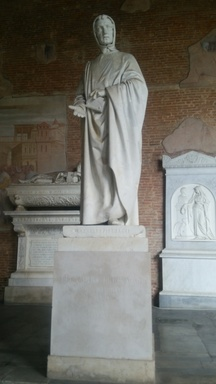
\includegraphics[width=.45\linewidth]{DSC_0537s.JPG}
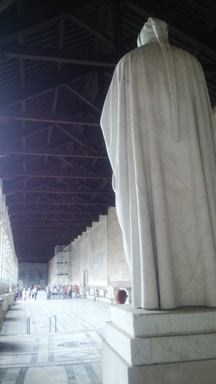
\includegraphics[width=.45\linewidth]{DSC_0541s.JPG}\\
\scriptsize フィボナッチ聖人の彫像\hfill(Camposanto, Pisa)
\end{minipage}

\end{tabular}


\section{数を数える}

\begin{psbox}{Fibonacci Number}{AOJ}
N番目のFibonacci数を求めよ。  

\url{http://judge.u-aizu.ac.jp/onlinejudge/description.jsp?id=ALDS1_10_A}
\end{psbox}

簡単のため$i$番目のFibonacci数を$F_i$と表記すると,以下のように定義される($F_0=0$と定義することも多いが本質ではないので問題文に合わせる):
\begin{equation}
  F_i = \left\{
  \begin{array}{ll}
    1 & i=0\\
    1 & i=1\\
    F_{i-1}+F_{i-2} & \mbox{(otherwise)}
  \end{array}\right.\label{eq:fib-recurrence}
\end{equation}

上記の定義をそのまま再帰で定義すると以下のようになるだろう:
\begin{pybox}
def fib(n):
    print("fib",n) # 関数呼び出しの際に引数を表示 (動作確認後に消す)
    if n == 0:
        return 0
    elif n == 1:
        return 1
    else:
        return fib(n-2)+fib(n-1)
\end{pybox}

しかし,この方法は計算の重複が多く,効率的でない.nの増加に伴い急速に遅くなる.
一例としてpythonの\tindex{timeit}モジュールを使った実行時間測定例を示す.
\begin{pybox}[emph=timeit]
import timeit
print(timeit.timeit("fib(10)", globals=globals(), number=10))
print(timeit.timeit("fib(20)", globals=globals(), number=10))
print(timeit.timeit("fib(30)", globals=globals(), number=10))
\end{pybox}

\begin{terminal}
$ python3 fib.py
0.0001415439764969051
0.01775405099033378
2.1516372300102375
\end{terminal}

今回主として扱う,より素直な方法は,小さいフィボナッチ数から順に計算す
ることである.
式(\ref{eq:fib-recurrence})から,$F_i$を求めるには,$F_0$から$F_{i-1}$までの値のみが必要であり,それらがあれば加算1回で計算できるという関係がわかる.そこで$F_0$から順に計算すれば,各$F_i$は加算1回で求められる.
\begin{cbox}
int F[100]; // 必要なだけ
int main() {
  F[0] = 1;
  F[1] = 1;
  for (int i=2; i<45; ++i) { // 必要なだけ
    F[i] = F[i-2]+F[i-1];
  }
}
\end{cbox}
この章で扱う問題は,求めたい問題の答え(e.g., $F_{100}$)が\jindex{部分問題}{ぶぶんもんだい}の答え($F_{n}, \; n<100$)から効率的に計算可能なものを取り扱う.
今回の場合は,回答にあたって直接必要なものは$N$番目のデータだけだが,一見回り道のようでも$N$番目*まで*のデータを全て計算しておくアプローチが有効である.
全体として必要な基本演算の回数(以下,単に計算量と表記する)は$O(N)$である.なお,メモ化や繰り返し自乗法による$O(\log N)$の計算方法については\footnote{簡単のために,この資料では整数演算のコストを定数と扱っている.しかし,多倍長整数を使う場合は,大きな数の演算は遅くなることに注意.},\ref{chapter:rsquares}章を参照されたい.

この節の目標は,部分問題の解の関係を表す,式(\ref{eq:fib-recurrence})のような漸化式から,解を求めるプログラムを書けるようになることである.


\begin{psbox}{Kannondou}{PC甲子園2007}
階段を1足で1,2,3段上がることができる人が,$n$ ($<30$)段登るときの登り方の数を,
適当に整形して出力する.

\aojid{0168}
\end{psbox}

各段への登り方の数を配列で表現する.
漸化式: 部分問題として,下から$i$段目に到達する登り方を$A_i$通りとする.登る前は
$A_0=1$, 最終的に知りたいのは$A_n$である.\\
\begin{equation}
  A_i = \left\{
  \begin{array}{ll}
    1 & i=0\\
    A_{i-1} & i=1\\
    A_{i-1}+A_{i-2} & i=2\\
    A_{i-1}+A_{i-2}+A_{i-3} & \mbox{(otherwise)}
  \end{array}\right.
\end{equation}

フィボナッチ数の計算と同様に,$N$段に対する答えを求める計算量は$O(N)$
となる.

回答例 (数の計算)
\begin{cbox}
#include <algorithm>
#include <iostream>
using namespace std;
int A[128], N;
int main() {
    A[0] = 1;
    for (int i=1; i<=32; ++i) {
        A[i] = A[i-1];
        if (...) A[i] += A[i-2];
        if (...) A[i] += A[i-3];
    }
    // A[.]を適当に出力してみる
}
\end{cbox}

\begin{pybox}
A = [0 for _ in range(32)]
A[0] = 1
for i in range(1,32):
    A[i] = A[i-1]
    if i > 1:
        A[i] += A[i-2]
        if i > 2:
            A[i] += A[i-3]  
\end{pybox}


\begin{debugbox}{配列の範囲外アクセスに注意}
  CやC++では配列の範囲外,たとえば\texttt{A[-1]},を参照したり書き込んだりしてはいけない(すぐに実行時エラーになるかもしれないし,ならないかもしれないし,もっと困ったことをしでかすかもしれない). 典型的には,\texttt{A[i-2]}にアクセスする文を書いたら,\texttt{i}$\le 1$では実行されないことをプログラマが保証する必要がある.
\end{debugbox}


回答例 (入出力)
\begin{cbox}
    while (cin >> N && N) 
        cout << ((A[N]+..)/10+...)/365 << endl;
\end{cbox}

整数で切り上げるには,割る前に除数-1を足せば良い.
Python3では整数除算には\texttt{//}を用いる.浮動小数と\texttt{ceil}を用いると計算誤差が発生しうるので注意.

\begin{pybox}
while True:
    n = int(input())
    if n == 0:
        break
    print(((A[n]+9)//10+364)//365)  
\end{pybox}


\begin{debugbox}{答えが合わない場合の参考}
   15段の場合は5768通りあり,2年かかる.
\end{debugbox}

\begin{pbox}{平安京ウォーキング}{UTPC2009}
  グリッド上の街をスタートからゴールまで,(ゴールに近づく方向にのみ歩く条件で)到達する経路を数える.ただし,マタタビの落ちている道は通れない.

  \aojid{2186}
\end{pbox}

なお,マタタビがなければ組み合わせ(目的地までに歩く縦横の道路の合計から縦の
道路をいつ使うか)の考え方から,直ちに計算可能である.

マタタビがある場合は,交差点毎に到達可能な経路の数を数えてゆくのが自然な解法で,
サンプル入力3つめの状況は,下の図のようになる.

\begin{center}
  \begin{tabular}{c@{\hspace{3em}}c}
      \begin{tikzpicture}[node distance=12mm]
        \node[city] (N11)                {$0,0$};
        \node[city] (N12) [below of=N11] {$0,1$};
        \node[city] (N13) [below of=N12] {$0,2$};
        \node[city] (N14) [below of=N13] {$0,3$};
        \node[city] (N21) [right of=N11] {$1,0$};
        \node[city] (N22) [below of=N21] {$1,1$};
        \node[city] (N23) [below of=N22] {$1,2$};
        \node[city] (N24) [below of=N23] {$1,3$};
        \node[city] (N31) [right of=N21] {$2,0$};
        \node[city] (N32) [below of=N31] {$2,1$};
        \node[city] (N33) [below of=N32] {$2,2$};
        \node[city] (N34) [below of=N33] {$2,3$};
        \node[city] (N41) [right of=N31] {$3,0$};
        \node[city] (N42) [below of=N41] {$3,1$};
        \node[city] (N43) [below of=N42] {$3,2$};
        \node[city] (N44) [below of=N43] {$3,3$};
        \node[city] (N51) [right of=N41] {$4,0$};
        \node[city] (N52) [below of=N51] {$4,1$};
        \node[city] (N53) [below of=N52] {$4,2$};
        \node[city] (N54) [below of=N53] {$4,3$};
        \path[->,thick] (N11) edge (N12);
        \path[->,thick] (N12) edge (N13);
        \path[->,thick] (N21) edge (N22);
        \path[->,thick] (N22) edge (N23);
        \path[->,thick] (N23) edge (N24);
        \path[->,thick] (N31) edge (N32);
        \path[->,thick] (N32) edge (N33);
        \path[->,thick] (N33) edge (N34);
        \path[->,thick] (N41) edge (N42);
        \path[->,thick] (N42) edge (N43);
        \path[->,thick] (N43) edge (N44);
        \path[->,thick] (N52) edge (N53);
        \path[->,thick] (N53) edge (N54);
        \path[->,thick] (N21) edge (N31);
        \path[->,thick] (N31) edge (N41);
        \path[->,thick] (N41) edge (N51);
        \path[->,thick] (N12) edge (N22);
        \path[->,thick] (N22) edge (N32);
        \path[->,thick] (N32) edge (N42);
        \path[->,thick] (N42) edge (N52);
        \path[->,thick] (N13) edge (N23);
        \path[->,thick] (N23) edge (N33);
        \path[->,thick] (N33) edge (N43);
        \path[->,thick] (N43) edge (N53);
        \path[->,thick] (N14) edge (N24);
        \path[->,thick] (N24) edge (N34);
        \path[->,thick] (N34) edge (N44);
      \end{tikzpicture}
&
      \begin{tikzpicture}[node distance=12mm]
        \node[city] (N11)                {$1$};
        \node[city] (N12) [below of=N11] {$1$};
        \node[city] (N13) [below of=N12] {$1$};
        \node[city] (N14) [below of=N13] {$0$};
        \node[city] (N21) [right of=N11] {$0$};
        \node[city] (N22) [below of=N21] {$1$};
        \node[city] (N23) [below of=N22] {$2$};
        \node[city] (N24) [below of=N23] {$2$};
        \node[city] (N31) [right of=N21] {$0$};
        \node[city] (N32) [below of=N31] {$1$};
        \node[city] (N33) [below of=N32] {$3$};
        \node[city] (N34) [below of=N33] {$5$};
        \node[city] (N41) [right of=N31] {$0$};
        \node[city] (N42) [below of=N41] {$1$};
        \node[city] (N43) [below of=N42] {$4$};
        \node[city] (N44) [below of=N43] {$9$};
        \node[city] (N51) [right of=N41] {$0$};
        \node[city] (N52) [below of=N51] {$1$};
        \node[city] (N53) [below of=N52] {$5$};
        \node[city] (N54) [below of=N53] {$5$};
        \path[->,thick] (N11) edge (N12);
        \path[->,thick] (N12) edge (N13);
        \path[->,thick] (N21) edge (N22);
        \path[->,thick] (N22) edge (N23);
        \path[->,thick] (N23) edge (N24);
        \path[->,thick] (N31) edge (N32);
        \path[->,thick] (N32) edge (N33);
        \path[->,thick] (N33) edge (N34);
        \path[->,thick] (N41) edge (N42);
        \path[->,thick] (N42) edge (N43);
        \path[->,thick] (N43) edge (N44);
        \path[->,thick] (N52) edge (N53);
        \path[->,thick] (N53) edge (N54);
        \path[->,thick] (N21) edge (N31);
        \path[->,thick] (N31) edge (N41);
        \path[->,thick] (N41) edge (N51);
        \path[->,thick] (N12) edge (N22);
        \path[->,thick] (N22) edge (N32);
        \path[->,thick] (N32) edge (N42);
        \path[->,thick] (N42) edge (N52);
        \path[->,thick] (N13) edge (N23);
        \path[->,thick] (N23) edge (N33);
        \path[->,thick] (N33) edge (N43);
        \path[->,thick] (N43) edge (N53);
        \path[->,thick] (N14) edge (N24);
        \path[->,thick] (N24) edge (N34);
        \path[->,thick] (N34) edge (N44);
      \end{tikzpicture}
\\
交差点の座標と通れる道 (右または下に移動可)
&
各交差点に到達可能な経路の数
 \end{tabular}
\end{center}

部分問題として,ある交差点に$(x,y)$に到達可能な経路数を考え,$T_{x,y}$と表記する.この値はそこに一歩で到達できる交
差点(通常は左と上)の値が定まっていれば,それらの和として計算可能である.

\begin{wrapfigure}[4]{l}[4pt]{3.5cm}

\includegraphics[width=3cm]{img/liftarn-Cat-silhouette.pdf}
\end{wrapfigure}

$$
T_{x,y} = \left\{
\begin{array}{l@{\hspace{3em}}l}
  0 & (x,y)\mbox{が範囲外}\\
  1 & (x,y) = (0,0)\\
  0 & \mbox{上にも左にもマタタビ}\\
  T_{x-1,y} & \mbox{上のみにマタタビ}\\
  T_{x,y-1} & \mbox{左のみにマタタビ}\\
  T_{x-1,y}+T_{x,y-1} & \mbox{上にも左にもマタタビなし}
\end{array}\right.
$$

マタタビの入力が多少冗長な形式で与えられるので,以下のように前処理して,移動不可能なことを示す配列などに格納しておくと使い勝手が良い.
\begin{itemize}
\setlength{\itemsep}{0pt}
\item x座標が同じ -- (x1, max(y1,y2)) には上から移動不可
\item y座標が同じ -- ((max(x1,x2), y1) には左から移動不可
\end{itemize}

たとえば,ある位置(x,y)に,上と左のそれぞれの方向からの移動できるかどうかを,\texttt{Vert[x][y]}と\texttt{Horiz[x][y]}の2つの二次元配列で管理する.
ある点(x,y)に上から移動可能であるなら\texttt{Vert[x][y]==true},そうでなければ\texttt{Vert[x][y]==false}とする.同様に,左から移動可能かで\texttt{Horiz[x][y]}の各要素を設定する.あらかじめ各要素を\texttt{true}に初期化しておき,マタタビがあった場合は\texttt{false}に書き換える.(移動*不可能*であることを表す場合は\texttt{true}と\texttt{false}の対応が逆になる.混乱しなければどちらでも良い.)



\begin{tipsbox}{プログラム作成手順のお勧め}
  各交差点に到達可能な経路の数を,前ページ図右のように全て表示し,手計算と一致するかどうかを確認しよう.
\end{tipsbox}
\begin{debugbox}{答えが合わない場合のヒント}
  またたびの縦横,上端や左端の扱い,$x_1 \le x_2$とは限らないこと($y_1,y_2$も)などに注意.
\end{debugbox}

\begin{tipsbox}{番兵法 (sentinel): 見通しの良いプログラムのヒント}
``Kannondou''の例題同様に,
  \texttt{x==0}で\texttt{T[x-1][y]}にアクセスしないようにすることと,
\texttt{y==0}の時\texttt{T[x][y-1]}にアクセスしないようにする必要がある.
\texttt{if}文で書くこともできるが,上端と左端に仮想的なマタタビがあると考えて\texttt{Vert[x][0]}と\texttt{Horiz[0][y]}を設定すると,簡潔に書くことができる.
\end{tipsbox}

\section{最適経路を求めて復元する}
\begin{pbox}{Spiderman}{Tehran 2003 Preliminary}
指定の高さH[i]だけ登るか降りるかを繰り返すトレーニングメニューを消化し
て地面に戻る.メニュー中で必要になる最大の高さを最小化する.

\url{http://poj.org/problem?id=2397}
\end{pbox}

この問題では,合計値ではなく最小値が必要とされる.    

$i$番目の上下移動を$H_i$($i$は0から),
$i$番目のビルで高さ$h$で居るために必要な最小コスト(=経路中の最大高さ)を $T_i[h]$とする.
それらの値を$T_0[0]=0$(スタート時は地上に居るので), 他を$\infty$で初期化した後,隣のビルとの関係から$T_i$と$T_{i+1}$を順次計算する.
$$T_{i+1}[h] = \min\left\{
\begin{array}{ll}
\max(T_i[h-H_i],h)  & \cdots i\mbox{番目のビルから登った場合} (h\ge H_i)\\
 T_i[h+H_i]  & \cdots \mbox{同降りた場合} 
\end{array}\right.
$$

ゴール地点を$M$として,ゴールでは地上に居るので,$T_M[0]$が最小値を与える.

\begin{wrapfigure}[5]{r}[4pt]{3.5cm}

\includegraphics[width=3cm]{img/buildings-icon.pdf}
\end{wrapfigure}       

地面に,めりこむことはないので,非負の高さのみを考える.また登り過ぎるとゴール地点に降りられなくなるので適当な高さまで考えれば良い.

さらに,この問題では最小値だけではなく最小値を与える\textbf{経路}が要
求される.どちらかの方法で求められる:
\begin{enumerate}
\setlength{\itemsep}{0pt}
\item 最小値$T_M[0]$を求めた後,ゴールから順にスタートに戻る.
隣のビルから登ったか降りたかは,$T_i$と$T_{i+1}$の関係から分かる.(両方同じ値ならどちらでも良い).
\item $T_{i+1}[h]$を更新する際に,登ったか降りたかを$U_{i+1}[h]$に記録
  しておく.$T_{M}[0]$を求めた後に,$U_{M}[0]$から順に$U_{M-1}[H_0]$までたどる
\end{enumerate}

\section{さまざまな動的計画法}

\paragraph{ナップサック問題}

価値と重さを持つ宝物がいくつかあるので,ナップサックの制限(運べる重さの
総合)を超えないように価値が高いものを選びたい.品物の種類と重さの取りうる数値の積が一定以内なら動的計画法で解くことが出来る.なお,液体のように自由に量を調
整できる場合は--全く別の問題であり--,重さあたりの価値が最も高いものから貪欲に選べば良い(動的計画法は不要である).

\begin{pbox}{Combinatorial - 0-1 Knapsack Problem}{AOJ}
各品物を最大1つまで選択できる0-1ナップザック問題で,制約を満たす価値の合計の最大値を求めよ.

\aojid{DPL_1_B}
\end{pbox}

\begin{wrapfigure}[4]{r}[4pt]{3.5cm}
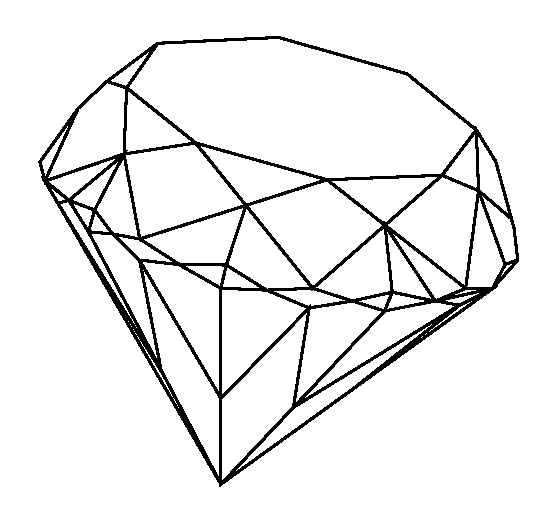
\includegraphics[width=3cm]{img/diamond-2.pdf}
\end{wrapfigure}

容量が整数で比較的小規模(配列に確保可能)な場合は,以下の方法が有力であ
る.まず品物に通し番号をつける(並び順は何でも良い).続いて,
部分問題として,品物$i$までしかない世界で,ナップサックの重さ制限が$c$
だった場合の,運べる価値の合計の最大値$V_{i,c}$を考える.
\begin{equation*}
    V_{i,c} = \left\{
  \begin{array}{ll}
    0 & i \le 0 \mbox{または} c \le 0\\
    V_{i-1,c} & c-\mbox{重さ}_i < 0 \\
    \max(\mbox{価値}_i + V_{i-1,c-\mbox{重さ}_i}, V_{i-1,c})
  \end{array}\right.
\end{equation*}
$V_{i,c}$は,$i$番目の品物を選ぶ場合と選ばない場合を考慮した最大値であるが,どちらの場合も$V_{i-1,*}$を用いて計算可能である.
そこで,二次元配列を利用して,全体の計算を効率よく行うことが出来る.
\pcaojbook[pp.~416--]参照.

\begin{center}
\begin{tikzpicture}
  \draw (15,11) -- (15,15) -- (10,15) -- (10,11);
  \draw[dashed] (10,14) -- (15,14);
  \node at (9.75,13.75) {i-1};
  \node at (9.75,13.25) {i};
  \draw (10,13.5) -- (15,13.5);
  \draw (10,13) -- (15,13);
  \draw[dotted,fill=black!30!white!70] (13.5,13.5) rectangle (14.0,14);
  \draw[dotted,fill=black!30!white!70] (11.5,13.5) rectangle (12.0,14);
  \draw[fill=gray] (13.5,13) rectangle (14.0,13.5);
  \node at (13.75,15.25) {c};
  \node at (11.75,15.25) {c-重さ${}_i$};
  \draw[ultra thick,->] (11.9,13.4) to [out=-30,in=210] (13.5,12.8);
  \draw[ultra thick,->] (14.1,13.8) to [out=-30,in=30] (14.1,13.1);
  \node at (14.6, 13.8) {+0};
  \node at (12.3, 12.5) {+価値${}_i$};
\end{tikzpicture}
\end{center}

\begin{pbox}{Combinatorial - Knapsack Problem}{AOJ}
各品物をいくつでも選択できるナップザック問題で,制約を満たす価値の合計の最大値を求めよ.

\aojid{DPL_1_C}
\end{pbox}

ほぼ同様の考え方になるが,漸化式が少し変化する.
この個数制限のないナップサック問題は,1個限定のナップサック問題と同じ計算量のオーダ$O(NW)$で解ける.もし,重さに関する\texttt{for}ループを一つ増やして三重ループにする方針をたてた場合は,$O(NW^2)$になる.改善を考えてみよう.

類題として,各item毎に個数制約(bound)が与えられている,個数制約付きナップサック問題も存在する.
スライド最小値の考え方を応用すると,(品物を増やした0-1 knapsackとして解くよりも)効率的に解を得られる(\pccbook[p.~302]も参照).

\paragraph{最長共通部分列と編集距離}
文字列などデータ列から,一部の要素を抜き出して並べた列(あるいは一部の
要素を消して詰めた列)を部分列という.二つのデータ列に対してどちらの部
分列にもなっている列を共通部分列という.共通部分列の中で長さが最大の列
を\jindex{最長共通部分列}{さいちょうきょうつうぶぶんれつ}と言う.最長共通部分列は複数存在する場合がある.

\begin{pbox}{Dynamic Programming - Longest Common Subsequence}{AOJ}
最長共通部分列の長さを求めよ

\aojid{ALDS1_10_C}
\end{pbox}

考え方: 文字列Xの先頭$i$文字部分を切り出した部分列を$X_i$と表す.$X_0$
は空文字列とする.文字列Xと文字列Yの最長共通部分列は,その部分問題であ
る$X_i$と$Y_j$の最長共通部分列の長さ$L_{i,j}$を利用して求めることが出来る.
\begin{equation*}
    L_{i,j} = \left\{
  \begin{array}{ll}
    0 & i \le 0 \mbox{または} j \le 0\\
    1 + L_{i-1,j-1} & \mbox{Xのi文字目とYのj文字目が同じ文字}\\
    \max(L_{i,j-1},L_{i-1,j}) & \mbox{otherwise}
  \end{array}\right.
\end{equation*}
この計算は二次元配列を利用して,効率よく行うことが出来る.
情報科学の「パターン認識」の章や\pcaojbook[pp.~253--]を参照.

補足: この問題は,Pythonでは制限時間に収めることが難しい.TLEの場合は,データをダウンロードして手元で答えを検証すると良い.

\begin{pbox}{Combinatorial - Edit Distance (Levenshtein Distance)}{AOJ}
  二つの文字列の編集距離を求めよ.
  
\aojid{DPL_1_E}
\end{pbox}


\paragraph{最長増加部分列}
最長増加部分列は動的計画法の有名問題の一つで,\texttt{vector}と二分探
索(\ref{section:binary-search}節参照)を組み合わせることで$O(N\log N)$で解くことが出来る.
問題末尾の解説
や\pcaojbook[pp.~421--]
参照.

\begin{pbox}{Combinatorial - Longest Increasing Subsequence}{AOJ}
  最長増加部分列 (Longest Increasing Subsequence)を求めよ.

\aojid{DPL_1_D}
\end{pbox}



\section{練習問題}

\begin{pbox}{Minimal Backgammon}{アジア地区予選2007}
直線上のすごろくでゴールできる確率を求めよ.
  
\aojid{1277}
\end{pbox}

\begin{pbox}{Coin Changing Problem}{AOJ}
ぴったり支払うときの,コインの最小枚数を求めよ.

\aojid{DPL_1_A}
\end{pbox}
注: 日本のコインは,大きなコインの額を小さいコインが割り切るという性質
があるため,大きなコインを使える限り使うほうが良い.つまり,支払額が
500円を超えていれば,500円玉を使うのが良い.一方,この問題はそうでない
状況も取り扱う.150円玉,100円玉,1円玉という硬貨のシステムで200円払うときには,150円玉を使うと枚数が最小ではない.
\pcaojbook[pp.~412--]参照.

\begin{pbox}{Eleven Lover$\star$}{模擬地区予選2009}
数字列中の11の倍数を数える
  
\aojid{2182}
\end{pbox}

方針例: 左から\textcolor{white}{ヒトケタづつ見てゆく.$i$桁目に注目するとして,$i$桁目で
終わる数で11で剰余を取ると$0\le j<11$になる数の個数を$A_{i,j}$とおく.$A_{i,.}$を$A_{i-1,.}$と$i$桁目の数値から}計算する.

\begin{pbox}{Restore Calculation$\star$}{アジア地区予選2013}
?を含む,二つの整数とその加算結果が与えられる.演算の整合性を満たすような?の埋め方が何通りあるか求めよ.

\aojid{2566}
\end{pbox}

\begin{pbox}{Magic Slayer$\star$}{夏合宿2009}
単体攻撃の魔法と全体攻撃の魔法を上手に使って,敵を全滅させろ.各魔法には,単体/全体の区別の他に,使用MPと与えるダメージ(Damage)が定められている.敵はいくつのダメージで倒されるかとしてHPの数値が与えられる.

\aojid{2156}
\end{pbox}

解説: \url{http://acm-icpc.aitea.net/index.php?plugin=attach&refer=2009%2FPractice%2F%B2%C6%B9%E7%BD%C9%2F%B9%D6%C9%BE&openfile=2b.pdf}

魔法の名前は無視して良い. 

単体魔法のみで敵が一体の場合を考える.合計でダメージ$d$を与えるのに必要なMPの最小値を$A_d$とすると

\begin{equation}
  A_d = \left\{
  \begin{array}{ll}
    0 & d\le 0\\
    \min_k(A_{d-\mbox{Damage}_k} + \mbox{MP}_k) & d > 0 \mbox{最後に魔法$k$を使った}
  \end{array}\right.
\end{equation}

敵$N$体を単体魔法のみで倒す場合は,それぞれのHPに必要な分を合計すれば良い.

全体魔法がある場合は,全体に合計ダメージ$d$を与えるのに必要な最小なMPを同様に計算し,組み合わせる.

\begin{pbox}{Mushrooms$\star$}{Algorithmic Engagements 2010}
直線を歩いてキノコを採集する.

\url{https://szkopul.edu.pl/problemset/problem/KVIxa_im2wGYJX99NB31p_nC/site/}
\end{pbox}

scanf推奨.


\begin{pbox}{輪番停電計画$\star$}{国内予選2011}
上手に区間を分割する.

\aojid{1176} 
\end{pbox}

長方形に対する値を管理するタイプ.

\begin{pbox}{Quest of Merchant$\star$}{夏合宿2011}
  様々な行動を総合して(問題文参照)収益を最大化せよ.

\aojid{2296}
\end{pbox}

\begin{pbox}{My friends are small}{夏合宿2010}
$N$個の荷物がある.重さの合計が$W$以下となる荷物の部分集合で,
極大なものの選び方は何通り? $N \le 200, W \le 10\,000$
\aojid{2333}
\end{pbox}

極大とは,選ばなかったどの荷物を加えても$W$を越える状態を意味する.

考え方: 選ばなかった荷物の\textcolor{white}{なかで,もっとも軽いもので場
  合分けする.合計の重さをwにする選び方が何通りかを計算するナップサック問題を,重い順に計算すると,解く過程の情報から解を得られる}

解説: \url{https://drive.google.com/file/d/1WC7Y2Ni-8elttUgorfbix9tO1fvYN3g3/view}

\begin{pbox}{Hakone$\star\star$}{夏合宿2012}
  (箱根駅伝の)順位変動(このチームは順位をあげて5位で通過などの情報)から,前の中継所での順位として何通り考えられるか求める.

\aojid{2439}
\end{pbox}




\begin{pbox}{Barricades}{Algorithmic Engagements 2007}
問題: 道路の一部をバリケードで塞いで連結なk都市を他の都市から侵入不能にしたい。

\url{https://szkopul.edu.pl/problemset/problem/1sX3vqLjiqkpxBNI-sh8UC2m/site/}
\end{pbox}

\begin{pbox}{Army Training$\star\star$}{Algorithmic Engagements 2010}

平面上の1000個までの点が与えられる.それらを適当につないで単純多角形を作った際に,領域に含まれる点の個数を数えよ.

\url{https://szkopul.edu.pl/problemset/problem/nXF1qOIv5S88utFPI2V_0gt3/site/}
\end{pbox}
 \chapter{分割統治}\label{chapter:divide-and-conquer}

\begin{itembox}[l]{概要}
分割統治法は,問題を小さな問題に再帰的に分解してそれぞれを解いたうえで,順次それらを組み合わせて全体の解を得る技法を指す.
元の問題より小さな問題を扱う点は動的計画法と共通だが,分割統治では分割した問題間に重なりがない場合を扱う.たとえば二分探索は分割統治の一つの手法であるが,フィボナッチ数の計算は分割統治とは通常呼ばれない.

この章では再帰(recursion)を取り扱う.再帰に慣れていない場合は,付録\ref{section:recursion}章を適宜参照のこと.
\end{itembox}

この章では、アイ(\texttt{i})とジェイ(\texttt{j})、イチ(\texttt{1})とエル(\texttt{l})が特に紛らわしいので注意のこと.



\section{二分探索}\label{section:binary-search}

問題を半分に分割して,片方のみを扱えば十分な場合として\jindex{二分探索}{にぶんたんさく}をみてみよう.
例として,辞書や名簿のように順番に並んでいるデータ列にある要素が存在するかどうかを判定する場合を考える.
たとえば``Moore''という姓を,全体が1024ページの名簿から探す場合に,
1024ページの真ん中の512ページから始める.そのページが ``M''より
  後なら,前を調べる. ``M''以前なら,後を調べる.いずれの場合でも,探す範囲を半分に絞ることが出来るといった具合である.

この探し方は,1ページ目から順に2,3ページと一ページづつ最終ページまで名簿を探すより,速い.
名簿のページ数を$n$とすると,調べるページ数は$O(n)$と$O(\log(n))$の差がある.

なお,次の節で紹介するマージソートや\texttt{inversion count}では,分割後に両方の領域について処理する必要がある.

\subsection{データ列中の値の検索}

C++の標準ライブラリに収められている\tindex{binary\_search}は整列済の配列から二分探索により要素の有無を判定する.

\begin{cbox}[emph={sort,binary_search}]
#include <iostream>
#include <algorithm>

sort(S, S+L); // 準備: 事前に配列S内を昇順に並び替えておく
...
    if (binary_search(S, S+L, a))) {
       // aがS内にある
    }
\end{cbox}

配列\texttt{A[]} から\texttt{value}を探す場合を多少形式的に書くと
\begin{enumerate}
\setlength{\itemsep}{0pt}
\item 調べる区間を$[l,r)$とする(範囲を表すには,left, right あるいは
  first, last などがしばしば用いられる).0ページ目から1023ページ目までを探す場合は,初期状態として\texttt{l=0, r=1024}とする
\item \texttt{l+n <= r}となったら,探す範囲は最大で\texttt{n}ページし
  か残っていないので,\texttt{[l,r)}の範囲を順に探す.(典型的には
    \texttt{n==1}, 実用的には \texttt{n==10}程度に取る場合もある.)
\item 区間の中央を求める \texttt{m=(l+r)/2}
\item \texttt{value < A[m]}なら(次は前半\texttt{[l,m)}を探したいので)\texttt{r=m},そう
  でなければ(\texttt{A[m] <= value} すなわち \texttt{A[m]==value}の場合を含む)後半\texttt{[m,r)}を探したいので\texttt{l=m}として2へ.(ここで\texttt{m==l}または{m==r}の場合は無限ループとなる.そうならないことを確認する.)
\end{enumerate}
というような処理となる.

\begin{cbox}[emph={left,right}]
bool bsearch(const int array[], int left, int right, int value) {
    // 前提:
    // - arrayは昇順に整列されている,
    // - 半開区間[left,right)は有効な範囲
    // 可能性
    // A. array[left] \(\le\) value \(\le\) array[right-1] (答えがありうる)
    // B. value \(\le\) array[left] (false確定)
    // C. array[right-1] \(\le\) value  (false確定)
    while (left + 1 < right) {
        // ループ不変条件: ループ開始時に成立したA,B,Cのどれかが終了時も成立
        int med = (left+right)/2;
        if (array[med] > value) right = med;
        else left = med;
    }
    return left < right && array[left] == value;
}
\end{cbox}

自分で二分探索を実装したら,Search IIで動作を確認することができる.

複雑なループを含むプログラムの正しさについて考える道具として,\cemph{ループ不変条件}という概念がある.必要に応じて,付録\ref{chapter:loop-invariants}章も参照のこと.

\begin{psbox}{Search II}{AOJ}
整数の配列S(売りたいリスト)とT(買いたいリスト)が与えられる.
Tに含まれる整数の中でSにも含まれる個数を出力せよ.

(入力の範囲)Sの要素数は10万以内,Tは5万以内.
SとTの要素数はそれぞれ100以内.配列に含まれる要素は,0以上$10^7$以下.

(注意)Tの要素は互いに異なるが,Sの要素は重複がある場合がある.


\aojid{10031}
\end{psbox}

\begin{debugbox}{問題の仕様に注意}
「Tの要素は互いに異なるが,Sの要素は重複がある場合がある」という意味は,
  \texttt{S=[1,1,1], T={1}}とすると答えは1ということである.
\end{debugbox}


\subsection{制約を満たす最小値を求める}

配列から値を探す状況以外にも,二分探索の考え方を用いると綺麗に解ける問題もある.

\begin{pbox}{Search - Allocation}{AOJ}
様々な重さの荷物を,並べられた順にトラックに積むことを考える.荷物の重さは並べられた順に配列\texttt{w}に格納してあるとする.
全てのトラックの最大積載量は同じとする.\texttt{k}台のトラックにすべての荷物を順に積む切るためには,各トラックの最大積載量は最低どれだけ必要か.
「トラックの最大積載量」の最小値を求めよ.

\aojid{ALDS1_4_D}
\end{pbox}

ヒント: トラックの最大積載量Pとして二分探索し,全ての荷物を積める最小値を求める.
求める値「積みきれる最小値」は(積載量が整数なので),「積みきれる最小値」=「積みきれない最大値」+1という関係から,「積みきれない最大値」を求める.
「積みきれない最大値」が存在する範囲を\texttt{[l,h)}で表現し,上限\texttt{h}を減らす条件を\texttt{ok}として表現する.求める答えは\texttt{h}となる.
\begin{cbox}[emph={l,h}]
bool ok(int P) {
  ... // 最大積載量Pのトラックに前から順に積み込んだ時の必要台数がK以内かを返す
}
int main() {
    // 問題読み込み
    int l = 0, h = // 大きな数;
    while (l+1 < h) {
        // loop不変条件: lでは積めない,hで積める
        int m = (l+h)/2;
        if (ok(m)) h = m; else l = m;
    }
    printf("
}
\end{cbox}

関数\texttt{ok}は,たとえば以下のように作成できる:
\begin{itemize}
\setlength{\itemsep}{0pt}
\item 現在のトラックに積んだ重さ(初期値0)とトラック台数(初期値1)を表す変数を作成
\item 各荷物について,現在のトラックに積んで最大積載量を超えないならそのまま積む(現在のトラックに積んだ重さを増やす)/そうでなければ新しいトラックに積む(トラックの台数を増やして,現在のトラックに積んだ重さをその荷物に設定)
\item 最後に台数をKと比較
\end{itemize}

\begin{pbox}{Aggressive Cows$\star{}$}{USACO 2005 February Gold}
直線上にN棟の牛舎(個室)がある.C頭の牛を,なるべく互いを離して入れたい.

(cinの代わりにscanfを使ってください)

\url{http://poj.org/problem?id=2456}
\end{pbox}

今回は条件を満たす最大値がほしいので,下限\texttt{l}を増やせる条件を関数\texttt{ok}として表現する.求める答えは\texttt{l}となる.
あらかじめ小屋の候補を昇順に並べてておくと,\texttt{ok}関数は,
\begin{itemize}
\setlength{\itemsep}{0pt}
\item 牛を左端の小屋に配置する (小屋がなければ失敗)
\item 距離M以内の小屋を考慮から消す
\end{itemize}
というステップを牛の数だけ繰り返し,全頭まで配置できれば成功として判定できる.


\begin{pbox}{Water Tank}{模擬地区予選2009}
タンクの容量と時間毎の水の使用量が与えられるので,最低限必要な給水速度を求める.(何周してもジリ貧にならない量が求められている)

(同名の別問題もあるので注意)

\aojid{2180}
\end{pbox}

ある給水速度を仮定した時に,それで生活できるかどうかを判定する関数を\texttt{ok}とする.求める速度を含む区間を$[\text{lo},\text{hi}]$で表現し,生活で
きるか出来ないかで範囲を半分に狭めてゆく.区間が十分狭くなったら終了し
て出力する.考え方と効果は二分探索(binary search)とほぼ同様だが,連続区間を扱う場合は二分法 (bisection)と呼ばれることが多い.

\begin{cbox}
  double lo = sum/86400, hi = 1e6; // 1e6 = $10^6$
  while (hi-lo>1e-6) {
      double m = (hi+lo)/2.0;
      if (ok(m)) hi = m;
      else lo = m;
  }
  printf("
\end{cbox}

原理は単純なのだが,関数\texttt{ok}の実装において
タンクの最大容量以上は水を貯められないなどの処理で慎重さが必要な点があるので,次の節のinversion countの問題のほう
が易しいかもしれない.

\section{Merge Sort}
分割統治の例として,Merge Sortという整列手法を取り上げる.この手法は,与えられた配列を半分に分割し,また元の大きさに組み立てる際に要素を整列する.図は,8,1,4,3,2,5,7,6という配列を整列する際の処理の流れを示している.上半分で分割し,下半分で整列が行われる.赤字は併合の際に右側から来た要素を示す.
具体的なソースコードは,次に紹介する\texttt{merge\_and\_count}とほぼ同様なので省略する.配列の要素数を$N$とすると,行が$O(\log{}N)$あり,各行あたりで必要な計算が$O(N)$なので,全体で$O(N\log{}N)$という計算量が導かれる.

\begin{center}
      \begin{tikzpicture}[node distance=18.4mm,
          merge/.style={
            draw=igreen,
            minimum size=7mm,
            ultra thick,
            inner sep=4pt
        }]
        \node[city] (A)              {8,1,4,3,2,5,7,6};
        \node[city] (B) [below left of=A] {8,1,4,3};
        \node[city] (C) [below right of=A] {2,5,7,6};
        \node[city] (E) [below left of=B] {4,3};
        \node[city] (D) [left of=E] {8,1};
        \node[city] (F) [below right of=C] {2,5};
        \node[city] (G) [right of=F] {7,6};
        \node[city] (I) [below left of=D] {1};
        \node[city] (H) [left of=I] {8};
        \node[city] (K) [below right of=E] {3};
        \node[city] (J) [left of=K] {4};
        \node[city] (L) [below left of=F] {2};
        \node[city] (M) [right of=L] {5};
        \node[city] (N) [below right of=G] {7};
        \node[city] (O) [right of=N] {6};
        \node[merge] (P) [below right of=I] {\textcolor{ired}{1},8};
        \node[merge] (Q) [right of=P] {\textcolor{ired}{3},4};
        \node[merge] (R) [below right of=L] {2,\textcolor{ired}{5}};
        \node[merge] (S) [right of=R] {\textcolor{ired}{6},7};
        \node[merge] (T) [below right of=Q] {1,\textcolor{ired}{3,4},8};
        \node[merge] (U) [below left of=R] {2,5,\textcolor{ired}{6,7}};
        \node[merge] (V) [below right of=T] {1,\textcolor{ired}{2},3,4,\textcolor{ired}{5,6,7},8};
        \path[->,thick] (A) edge (B);
        \path[->,thick] (A) edge (C);
        \path[->,thick] (B) edge (D);
        \path[->,thick] (B) edge (E);
        \path[->,thick] (C) edge (F);
        \path[->,thick] (C) edge (G);
        \path[->,thick] (D) edge (H);
        \path[->,thick] (D) edge (I);
        \path[->,thick] (E) edge (J);
        \path[->,thick] (E) edge (K);
        \path[->,thick] (F) edge (L);
        \path[->,thick] (F) edge (M);
        \path[->,thick] (G) edge (N);
        \path[->,thick] (G) edge (O);
        \path[->,thick] (H) edge (P);
        \path[->,thick] (I) edge (P);
        \path[->,thick] (J) edge (Q);
        \path[->,thick] (K) edge (Q);
        \path[->,thick] (L) edge (R);
        \path[->,thick] (M) edge (R);
        \path[->,thick] (N) edge (S);
        \path[->,thick] (O) edge (S);
        \path[->,thick] (P) edge (T);
        \path[->,thick] (Q) edge (T);
        \path[->,thick] (R) edge (U);
        \path[->,thick] (S) edge (U);
        \path[->,thick] (T) edge (V);
        \path[->,thick] (U) edge (V);
      \end{tikzpicture}
\end{center}

\subsection{Inversion Count}

配列内の要素のペアで,\texttt{A[i] > A[j] (i<j)}のものを数えたい.
例えば配列\texttt{[3 1 2]} の中には (3,1)と(3,2)の二つのペアの大小関係が逆転している.
愚直に次のようなコードを書くと,要素数$N$の自乗に比例する時間がかかる$O(N^2)$.

\begin{cbox}
int N, A[128];
int solve() {
    int sum = 0;
    for (int i=0; i<N; i++)
        for (int j=i+1; j<N; j++)
            if (A[i] > A[j]) ++sum;
    return sum;
}
\end{cbox}

Merge sortの応用で,半分に分割しながら数えると,$O(N\log N)$で求めることができる.

\begin{cbox}[emph={merge_and_count}]
int N, A[たくさん]; // Aは元の配列
int W[たくさん]; // Wは作業用配列
int merge_and_count(int l, int r) { // range [l,r)
    if (l+1 >= r) return 0; // empty
    if (l+2 == r) { // [l,r) == [l,l+1] 要素2つだけ
        if (A[l] <= A[l+1]) return 0;  // 逆転はなし
        swap(A[l], A[l+1]);
        return 1; // 逆転一つ
    }
    int m = (l+r)/2; // [l,r) == [l,m) + [m,r)
    int cl = merge_and_count(l, m); // 左半分を再帰的に数える
    int cr = merge_and_count(m, r); // 右半分を再帰的に数える
    int c = 0; // 左と右を混ぜるときの逆点数
    int i=l, j=m; // iは[l,m)を動き, jは[m,r)を動いて,
    int k=l;      // 小さいものからW[k]に書き込む
    while (i<m && j<r) { // A[i]とA[j]を比べながら進む
        if (A[i] <= A[j]) W[k++] = A[i++]; // 左半分の方が小さく逆転なし
        else {
            W[k++] = A[j++];
            c += XXX; // 左半分の方が大きい,左半分で未処理の要素だけ飛び越える
        }
    }
    while (i<m) W[k++] = A[i++]; // 左半分が余った場合
    while (j<r) W[k++] = A[j++]; // 右半分が余った場合
    assert(k == r);
    copy(W+l, W+r, A+l);
    return cl + cr + c;
}
\end{cbox} 

\subsection{練習問題}


\begin{pbox}{Recursion / Divide and Conquer - The Number of Inversions}{AOJ}
与えられた数列内の,大小関係が逆転しているペアの個数を求める

\aojid{ALDS1_5_D}
\end{pbox}

\begin{pbox}{Ultra-QuickSort}{Waterloo local 2005.02.05}
類題: 数が大きいのでlong longを使うこと.

\url{http://poj.org/problem?id=2299} 
\end{pbox}

\begin{pbox}{Japan$\star$}{Southeastern Europe 2006}
長方形の島の東西に道路が走っている.交わる箇所の数を求めよ

\url{http://poj.org/problem?id=3067}
\end{pbox}

解き方の例: (東, 西)のペアでソートすると前2問と同じ問題になる.この問題は,累積和を管理しても解ける.

\section{木のたどり方}

\begin{center}
\begin{tabular}{c}
  \begin{forest}
    ctree [$D_{1,7,13}$ [$B_{2,4,6}$ [$A_3$] [$C_5$]] [$E_{8,12}$
        [nil,cnil] [$G_{9,11}$ [$F_{10}$], [nil,cnil]]]]
  \end{forest}
\\
例1: 数字は訪問順序を表す
\end{tabular}
\end{center}

根から始めて,下のような再帰的な手続き(深さ優先探索,\ref{section:graphsearch}章)で,辺をたどりながら各頂点を一巡することを考える:
\begin{enumerate}
\setlength{\itemsep}{0pt}
\item 左の子が存在し,かつ未訪問なら,左の子を訪問する
\item (そうではなくて)右の子が存在し,かつ未訪問なら,右の子を訪問する
\item (そうではなくて)親があれば,親へ戻る
\item いずれでもなければ,(根に帰ってきたので)終了
\end{enumerate}

図の「例1」の木であれば,DBABCBDEGFGED と通る.
例から分かるように,子供をもつ頂点は複数回(正確には次数)通過する.

この訪問順を基本としたうえで,各頂点を一度だけ処理する方法として,
preorder (自分, 左, 右), inorder (左, 自分, 右), postorder
(左, 右, 自分)などが用いられる.それぞれの方法では,子供と自分の優先順位が異なる.

\begin{center}  
\begin{tabular}{ll}\hline
 & DBABCBDEGFGED\\\hline
preorder & DBA\phantom{B}C\phantom{B}\phantom{D}EGF\phantom{GED}\\
inorder  & \phantom{DB}ABC\phantom{B}DE\phantom{G}FG\phantom{ED}\\
postorder &\phantom{DB}A\phantom{B}CB\phantom{DEG}FGED\\
\hline
\end{tabular}
\end{center}

\begin{pbox}{Tree - Reconstruction of a Tree}{AOJ}
ある二分木について, preorder (root, left, right) で出力した頂点のリス
トと,inorder (left, root, right) で出力したリストが与えられる.
(元の木を復元し)その頂点をpostorder (left, right, root) で出力せよ.
なお,元の木で,異なる頂点には異なるラベルがついている.

  \aojid{ALDS1_7_D}
\end{pbox}

\begin{pbox}{Tree Recovery$\star$}{Ulm Local 1997}
上に同じ(複数ケースが与えられる点と,書式が少し異なる)

\url{http://poj.org/problem?id=2255}  
\end{pbox}


ヒント:
\begin{itemize}
\setlength{\itemsep}{0pt}
\item ルートをA, その左側の部分木をL (nullの場合もある), 右部分をRとす
  る.preorderでは,AL'R' のように並んでいる.(L'とR'はそれぞれの
  preorder表記). inorderでは,L''AR''のように並ぶ(L''とR''はそれぞれの
  inorder表記)
\item preorder表記の先頭から直ちに,ルートAが特定できる
\item L, R部分は,inorder表記からAを探すことによって,要素を特定できる
\item 文字数は,L'とL'', R'とR''で等しいことに注意
\item L'とL''から,左側の木を復元する問題は,元の問題の小さくなったバージョンである.
\end{itemize}

回答例:

\begin{cbox}
#include <iostream>
#include <string>
using namespace std;
string preorder, inorder;
// preorder の[fp,lp) の範囲と,inorderの [fi,li)の範囲について
// 木をpostorderで表示
void recover(int fp, int lp, int fi, int li) {
    int root;
    // preorder[fp] == inorder[root]となるようなrootを求める
    if // (左側が存在すれば)
      recover(fp+1, fp+(root-fi)+1, fi, root); // 左側を表示
    if // (右側が存在すれば)
      recover(fp+(root-fi)+1, lp, root+1, li); // 右側を表示
    cout << inorder[root]; // root を表示
}
int main() {
    while (cin >> preorder >> inorder) {
        recover(0, preorder.size(), 0, inorder.size());
        cout << endl;
    }
}
\end{cbox}

呼び出し関係を図にすると,以下のようになる.図中,赤字が(その時点での
部分木における)根を表す.頂点内の文字列は,その頂点以下の部分木に対す
る,preorder表記(上段, fpとlpの範囲)とinorder表記(下段, fiとliの指す範囲).


\begin{center}
\begin{forest}
  sn edges
  [\vbox{\hbox{\textcolor{ired}{D}BACEGF}\hbox{ABC\textcolor{ired}{D}EFG}}
  [\vbox{\hbox{\textcolor{ired}{B}AC}\hbox{A\textcolor{ired}{B}C}}
    [A][C]]
  [\vbox{\hbox{\textcolor{ired}{E}GF}\hbox{\textcolor{ired}{E}FG}}
  [nil,cnil]
  [\vbox{\hbox{\textcolor{ired}{G}F}\hbox{F\textcolor{ired}{G}}} [F] [nil,cnil]]]]
\end{forest}
\end{center}


\section{空間充填曲線}
\begin{pbox}{Recursion / Divide and Conquer - Koch Curve}{AOJ}
  \begin{minipage}{.7\linewidth}
コッホ曲線の頂点を計算せよ.
  
\aojid{ALDS1_5_C}
  \end{minipage}
\begin{tikzpicture}[decoration=Koch snowflake]
    \draw decorate{ decorate{ decorate{ decorate{ (0,0) -- (3,0) }}}};
\end{tikzpicture}
\end{pbox}

ヒント: 基準線が$(x0,y0)$から$(x0+dx,y0+dy)$に引かれるとき,左手側にこぶを作るには,中点$(x0+dx/2,y0+dy/2)$から,$(-dy,dx)$方向に適当な距離を伸ばせば良い.

\jindex{コッホ曲線}{こっほきょくせん}を描く再帰関数の設計には2通りの方針がある: 一つは表示させる設計,もう一つは点列を返す設計である.

関数\tindex{koch}\texttt{(x0,y0,x1,y1,n)}を,「座標(x0,y0)から(x1,y1)までの点を表示する(端点は(x0,y0)を含み(x1,y1)を含まない)」と設計すると,以下のような構造になる:
\begin{pybox}
import math
def show_vertex(x,y):
    print("
def koch(x0,y0, x1,y1, n):
    if n == 0:
        show_vertex(x0,y0)
    else:
        ... # 中間点c1,c2,c3を計算
        koch(x0,y0, c1[0],c1[1], n-1)
        koch(c1[0],c1[1], c2[0],c2[1], n-1)
        koch(c2[0],c2[1], c3[0],c3[1], n-1)
        koch(c3[0],c3[1], x1,y1, n-1)

N = int(input())
koch(0,0,100,0,N)
show_vertex(100,0)
\end{pybox}

点列を返す場合は,以下のように書ける(全体の計算終了後に最後にまとめて表示する):
\begin{pybox}
def koch(x0,y0, x1,y1, n):
    if n == 0:
        return [(x0,y0)]
    else:
        ... # 中間点c1,c2,c3を計算
        return koch(x0,y0, c1[0],c1[1], n-1) \
            + koch(c1[0],c1[1], c2[0],c2[1], n-1) \
            + koch(c2[0],c2[1], c3[0],c3[1], n-1) \
            + koch(c3[0],c3[1], x1,y1, n-1)

def show_vertex(x,y):
    print("

N = int(input())
V = koch(0,0,100,0,N)+[[100,0]]
for x,y in V:
    show_vertex(x,y)
\end{pybox}

C++では,後者の設計の実装は面倒があるので,前者の設計(再帰関数の中で表示)が簡便である.

\begin{tipsbox}{点列の図示}
  答えが合わないときや,方針に悩んだ時は点列を図示すると良い.
\tindex{gnuplot}が利用可能な環境では,次の手順で単に図示できる.
(1) ターミナルでgnuplotを起動する (2) gnuplotのプロンプトで\texttt{plot 'xy.txt' with lines}とタイプする.ただし,プログラムが出力した座標を ``xy.txt''に保存したとする.
\begin{terminal}
$ gnuplot
gnuplot> plot 'xy.txt' with lines
\end{terminal}
\end{tipsbox}
  またPythonの場合は,\tindex{matplotlib}を使うと便利である.
\begin{pybox}
import matplotlib.pyplot as plt
import numpy as np
def plot_koch(a):
    fig = plt.figure()
    ax = fig.add_subplot(1,1,1)
    a_ = np.array(a)
    xlist = a_[:, 0]
    ylist = a_[:, 1]
    ax.plot(xlist, ylist)
    ax.set_title('koch curve')
\end{pybox}
(jupyter内で表示するには,先頭で\texttt{\%matplotlib inline}を実行しておく)

\begin{pbox}{Riding the Bus$\star\star$}{世界大会 2003}

正方形内に描かれたPeano curve上に格子点がある.与えられた二点間の距離を求めよ.距離とは,与えられた点から最短の格子点への距離(複数ある場合はx,y座標が小さいものまで)と,格子点間のPeano curve上の道のり.(誤差の記述がちょっと心配)

\url{https://icpcarchive.ecs.baylor.edu/index.php?option=com_onlinejudge&Itemid=8&category=37&page=show_problem&problem=724}
\end{pbox}

解き方の例: 全体を9分割して,関係ある場所だけを細かく探す.

\begin{pbox}{Plotter$\star\star$}{Algorithmic Engagements 2011}
与えられた点をいつペンが通るか.
  
\url{http://main.edu.pl/en/archive/pa/2011/plo}
\end{pbox}
 \chapter{基本データ構造(string, stack, queue, string, set, map)}\label{chapter:datastructure}

\begin{itembox}[l]{概要}
この章では,C++やJavaなど多くの言語で標準ライブラリとして提供されている
「道具」として,文字列,スタック,(優先度付き)キュー,集合,連想配列を
紹介する.道具の紹介が退屈な読者は,一旦飛ばして先に進んでおいて,あと
で必要になってから戻ってくる読み方も可能である.なお,この資料では,ま
ず標準ライブラリを使いこなすことを勧める立場を取る.これらの道具を自作
することも筋力トレーニングとしては有用であるが,初学者には向かない.また実
用的な状況では,標準ライブラリで用が足りるならその方が望ましい.
たとえば,多くの人に使われているのでバグがないなどのメリットが期待される,他の人も性質を良く
知っているため共同作業に向いている,などの利点がある.

なお,この章では,C++とPython3についてサンプルコードを取り上げる.Rubyについては,付録\ref{chapter:ruby}を参照.
\end{itembox}

\section{文字列(string)と入出力}

\begin{cbox}[emph={string}]
#include <iostream>
#include <string>
using namespace std;
int main() {
  string word; // 文字列型の変数wordを定義
  cin >> word; // 標準入力から一単語読み込む(空白や改行文字で区切られる)
  cout << word << word << endl; // 2回表示する
}  
\end{cbox}

\texttt{hello}(改行)と入力すると\texttt{hellohello}と出力される.

C++のstringクラスは,Cの文字列よりもかなり便利なので,早めに慣れておく
ことをお勧めする.

\begin{cbox}
#include <string>
  string word; // 定義
  string word2="ABCD"; // 定義と同時に初期化
  word = "EF"; // 代入
  string word3 = word + word2; // 連結
  char c = word[n]; // n文字目を取り出す
  word[n] = 'K'; // n文字目に代入 (\texttt{n<word.size()}でないと破綻)
  cin >> word; // 一単語読み込み(改行や空白文字で分割される)
  cout << word.size() << endl; // 文字数表示
  if (word.find("A") != string::npos) ... // もしwordにAが含まれるなら...
\end{cbox}

\begin{pybox}
word = input().strip()
print(word*2)
\end{pybox}

1単語読み込むことと1行読み込むことは意味が異なるが,今回は違いに踏み込まない.


\section{スタック(stack)とキュー(queue)}

スタックとキュー(\pcaojbook[pp.~80--], \pccbook[pp.~31--])は,データを一時的に保存したり取り出したりするためのデー
タ構造である.どちらもデータを1列に並べて管理して,新しいデータを列の
(どちらかの)端に保存し,また取り出す際も(どちらかの)端から取り出す.

\jindex{スタック}{すたっく}は,後に保存したデータを,先に取り出すデータ構造である.たとえ
ば,仕事をしている最中に急な案件が発生したので,今取り組んでいる仕事を
「仕事の山」の先頭に積んでおいて,急な案件を処理し,それが終わったら仕
事の山の先頭から再び処理を続けるような状況で有用である.もちろん急な案
件の処理中に,さらに急な案件が発生した場合も同様に仕事の山に積んだり下
ろしたりする.

\jindex{キュー}{きゅー}は,先に保存したデータを,先に取り出すデータ構造である.飲食店に
到着した人は列の後ろに並び,列の中で一番早く到着した人から順に店内に案
内される状況に相当する.


\jindex{優先度付きキュー}{ゆうせんどつききゅー}では,早く並んだ順ではなく各データの優先度の高い順に取り出される.現実にはぴったりした例がないが,待っている人の中から優先度の高い順に診療が行われるような状況や,高い買値を提示した順に品物を入手できる市場などがもしあれば相当するだろう.


なお,C++の標準ライブラリで提供されているでは取り出し操作が,先頭要素の参照\texttt{top()}あるいは\texttt{front()}と先頭要素の削
除\texttt{pop()}という二つの操作に分離されていることに注意\footnote{こ
  れはexception safetyのためである.}.通常の使用状況では,先頭の要素を得つつスタックやキューからは取り除きたいので,両者の操作を
続けて行う.


\subsection{スタック}\label{section:stack}

\paragraph{概要}
スタック(\eindex{stack})は,\tindex{push}\texttt{()}と\tindex{pop}\texttt{()}という二つの操作を提供する
データ構造である.
それぞれ,データの追加と,取り出しを行う.
現在先頭にあるデータは,\tindex{top}\texttt{()}で参照できる.

\centerline{\begin{tabular}{c@{\hspace{2em}}c@{\hspace{2em}}c@{\hspace{2em}}c@{\hspace{2em}}c}
\imagetop{\begin{tikzpicture}
\phantom{\draw (0,1.4) -- (0,0);}
\draw[thick] (0,0) -- (2,0);
\end{tikzpicture}}
&
\imagetop{\begin{tikzpicture}
\phantom{\draw (0,1.4) -- (0,0);}
\draw[ultra thick,->] (0.25,1) -- (0.8,0.2) node [above right,rotate=30] {push 3};
\draw[thick] (0,0) -- (0.5,0) -- (0.5,-.5) -- (1.5,-.5) -- (1.5,0) -- (2,0);
\draw[dotted] (0.5,0) -- (1.5,0);
\node at (1,-0.25) {$3$};
\end{tikzpicture}}
&
\imagetop{\begin{tikzpicture}
\phantom{\draw (0,1.4) -- (0,0);}
\draw[ultra thick,->] (0.25,1) -- (0.8,0.2) node [above right,rotate=30] {push 4};
\draw[thick] (0,0) -- (0.5,0) -- (0.5,-1) -- (1.5,-1) -- (1.5,0) -- (2,0);
\draw[dotted] (0.5,0) -- (1.5,0);
\draw[dotted] (0.5,-0.5) -- (1.5,-0.5);
\node at (1,-0.25) {$4$};
\node at (1,-0.75) {$3$};
\end{tikzpicture}}
&
\imagetop{\begin{tikzpicture}
\phantom{\draw (0,1.4) -- (0,0);}
\draw[ultra thick,->] (0.25,1) -- (0.8,0.2) node [above right,rotate=30] {push 1};
\draw[thick] (0,0) -- (0.5,0) -- (0.5,-1.5) -- (1.5,-1.5) -- (1.5,0) -- (2,0);
\draw[dotted] (0.5,0) -- (1.5,0);
\draw[dotted] (0.5,-0.5) -- (1.5,-0.5);
\draw[dotted] (0.5,-1) -- (1.5,-1);
\node at (1,-0.25) {$1$};
\node at (1,-0.75) {$4$};
\node at (1,-1.25) {$3$};
\end{tikzpicture}}
&
\imagetop{\begin{tikzpicture}
\phantom{\draw (0,1.4) -- (0,0);}
\draw[ultra thick,<-] (0.25,1) -- (0.8,0.2) node [above right,rotate=30] {pop};
\draw[thick] (0,0) -- (0.5,0) -- (0.5,-1) -- (1.5,-1) -- (1.5,0) -- (2,0);
\draw[dotted] (0.5,0) -- (1.5,0);
\draw[dotted] (0.5,-0.5) -- (1.5,-0.5);
\node at (1,-0.25) {$4$};
\node at (1,-0.75) {$3$};
\end{tikzpicture}}
\\
(empty) & top$=3$ & top$=4$ & top$=1$ & top$=4$
\end{tabular}}

\paragraph{使用上の注意}
通常は,配列や\texttt{vector}などが用いられる.
典型的な実装での計算コストは\texttt{push()},\texttt{pop()},\texttt{top()}とも定数時
間である.つまり,データがどれだけ増えても,各操作の計算時間は増えないと期待される.

なお,\texttt{pop()}が\texttt{top()}同様に値を返す実装もあるが,C++の
標準ライブラリで提供されているものはでは,両者が分離されていることに注意\footnote{こ
  れはexception safetyのためである.}.通常の使用状況では,先頭の要素を得つつスタックやキューからは取り除きたいので,両者の操作を
続けて行う.

また現在の要素数を調べる\texttt{size()}などのメンバ関数も提供されているので詳しくは文法書を参照のこと\footnote{ウェブにも資料がある\url{http://en.cppreference.com/w/cpp/container/stack}}.

\begin{cbox}[emph={stack,push,top,pop}]
#include <stack>
#include <iostream>
using namespace std;
int main() {
    stack<int> S; // intを格納するスタック
    S.push(3); // 先頭に追加
    S.push(4);
    S.push(1);
    while (! S.empty()) { // 要素がある間
	int n = S.top(); // 先頭をコピーして
	S.pop(); // 先頭要素を廃棄
	cout << n << endl; // 1, 4, 3  の順に表示される
    }
}  
\end{cbox}

Pythonでは\texttt{append, pop}をそれぞれ\texttt{push, pop}として用いる
ことにする.
\begin{pybox}[emph={append,pop}]
stack = []
stack.append(3)
stack.append(4)
stack.append(1)
while len(stack) > 0:
    n = stack.pop()
    print(n)
\end{pybox}

\begin{psbox}{Reverse Polish Notation}{AOJ}
「逆ポーランド記法」で与えられる文法を読んで、値を計算する
  
\aojid{ALDS1_3_A}
\end{psbox}

ヒント: 問題分末尾にある「解説」も参照.
\pcaojbook[p.82]に詳しい解説が掲載されている.

\begin{cbox}[emph={string,stack,top,push}]
#include <string>
#include <stack>
#include <iostream>
using namespace std;
int main() {
  string word;
  stack<int> S;
  while (cin >> word) { // 入力がある限り読み込む
    if (word == "+") {
      // 数を2つpopして、和をpushする
    }
    else if (word == "-") {
      // 数を2つpopして、差をpushする
    }
    else if (word == "*") {
      // 数を2つpopして、積をpushする
    }
    else {
      // wordを数値にしてpushする
    }
  }
  // Sの先頭要素を表示する。
}
\end{cbox}

このプログラムは入力が続くかぎり読み込む。キーボードから入力の終わりを
与えるには ``\textasciicircum{}D'' (Ctrlキーを押しながら ``d''を押す)を用いる。

数をあらわす文字列を整数\texttt{n}に変換するには、
C++11の場合は \texttt{int n=stoi(word)}を、
そうでない場合は \texttt{<cstdlib>} をincludeして、\texttt{int n=atoi(word.c\_str())}などとする。(AOJのC++11はまだ\texttt{stoi}をサポートしていないので\texttt{atoi}を用いる)

\begin{pbox}{Largest Rectangle in a Histogram}{Ulm Local 2003}
  ヒストグラム中に含まれる最大の長方形の面積を求めよ.(long long注意)

\url{http://poj.org/problem?id=2559}
\end{pbox}

スタックをうまく活用すると,ヒストグラムの本数に比例する手間で求められ
る.

参考: \url{http://algorithms.blog55.fc2.com/blog-entry-132.html}

\subsection{キュー}\label{section:queue}
\paragraph{概要} キュー(\eindex{queue},\pccbook[p.~32])は,
データの格納(\texttt{push()})と取り出し(\texttt{pop()})ができるデータ構造である.
現在先頭にあるデータは,\tindex{front}\texttt{()}で参照する.

\centerline{\begin{tabular}{c@{\hspace{2em}}c@{\hspace{2em}}c@{\hspace{2em}}c@{\hspace{2em}}c}
\imagetop{\begin{tikzpicture}
\phantom{\draw (0,1.0) -- (0,0);}
\draw[thick] (0,0) -- (2,0);
\end{tikzpicture}}
&
\imagetop{\begin{tikzpicture}
\phantom{\draw (0,1.0) -- (0,0);}
\draw[ultra thick,->] (0.25,-1.5) -- (0.8,-0.7) node [below right,rotate=-30] {push 3};
\draw[thick] (0,0) -- (0.5,0) -- (0.5,-.5) -- (0,-.5);
\draw[thick] (2,-.5) -- (1.5,-.5) -- (1.5,0) -- (2,0);
\draw[dotted] (0.5,0) -- (1.5,0);
\draw[dotted] (0.5,-0.5) -- (1.5,-0.5);
\node at (1,-0.25) {$3$};
\end{tikzpicture}}
&
\imagetop{\begin{tikzpicture}
\phantom{\draw (0,1.0) -- (0,0);}
\draw[ultra thick,->] (0.25,-2) -- (0.8,-1.2) node [below right,rotate=-30] {push 4};
\draw[thick] (0,0) -- (0.5,0) -- (0.5,-1) -- (0,-1);
\draw[thick] (2,-1) -- (1.5,-1) -- (1.5,0) -- (2,0);
\draw[dotted] (0.5,0) -- (1.5,0);
\draw[dotted] (0.5,-0.5) -- (1.5,-0.5);
\draw[dotted] (0.5,-1) -- (1.5,-1);
\node at (1,-0.25) {$3$};
\node at (1,-0.75) {$4$};
\end{tikzpicture}}
&
\imagetop{\begin{tikzpicture}
\phantom{\draw (0,1.0) -- (0,0);}
\draw[ultra thick,->] (0.25,-2.5) -- (0.8,-1.7) node [below right,rotate=-30] {push 1};
\draw[thick] (0,0) -- (0.5,0) -- (0.5,-1.5) -- (0,-1.5);
\draw[thick] (2,-1.5) -- (1.5,-1.5) -- (1.5,0) -- (2,0);
\draw[dotted] (0.5,0) -- (1.5,0);
\draw[dotted] (0.5,-0.5) -- (1.5,-0.5);
\draw[dotted] (0.5,-1) -- (1.5,-1);
\draw[dotted] (0.5,-1.5) -- (1.5,-1.5);
\node at (1,-0.25) {$3$};
\node at (1,-0.75) {$4$};
\node at (1,-1.25) {$1$};
\end{tikzpicture}}
&
\imagetop{\begin{tikzpicture}
\phantom{\draw (0,1.0) -- (0,0);}
\draw[ultra thick,->] (0.75,0.2) -- (1.3,1) node [below right,rotate=-30] {pop};
\draw[thick] (0,0) -- (0.5,0) -- (0.5,-1) -- (0,-1);
\draw[thick] (2,-1) -- (1.5,-1) -- (1.5,0) -- (2,0);
\draw[dotted] (0.5,0) -- (1.5,0);
\draw[dotted] (0.5,-0.5) -- (1.5,-0.5);
\draw[dotted] (0.5,-1) -- (1.5,-1);
\node at (1,-0.25) {$4$};
\node at (1,-0.75) {$1$};
\end{tikzpicture}}
\\
(empty) & front$=3$ & front$=3$ & front$=3$ & front$=4$
\end{tabular}}

\paragraph{使用上の注意}
実装には,配列や\tindex{deque}が用いられる.
計算コストは\texttt{push()},\texttt{pop()},\texttt{front()}とも定数時
間である.つまり,データがどれだけ増えても,各操作の計算時間は増えないと期待される.
(データ全体を移動させると$O(N)$かかってしまうので,実際にはheadとtailのような現在使用中の区間をあらわす添字またはポインタのみを操作する).

C++では,queueというテンプレートクラスが用意されている.入れた(pushし
た)データを,front()及びpop()の操作により取り出す.\footnote{\url{http://en.cppreference.com/w/cpp/container/queue}}
\begin{cbox}[emph={queue,push,front,pop}]
#include <queue>
#include <iostream>
using namespace std;
int main() {
    queue<int> Q; // intを格納するキュー
    Q.push(3); // 末尾に追加
    Q.push(4);
    Q.push(1);
    while (! Q.empty()) { // 要素がある間
	int n = Q.front(); // 先頭をコピーして
	Q.pop(); // 先頭要素を廃棄
	cout << n << endl; // 3, 4, 1  の順に表示される
    }
}
\end{cbox}

Pythonのqueueの表現としては,この資料では\texttt{collections.deque}の\texttt{append, popleft}を用いることにする.\footnote{https://docs.python.jp/3/library/collections.html\#deque-objects}
\begin{pybox}[emph={append,popleft}]
import collections
q = collections.deque()
q.append(3)
q.append(4)
q.append(1)
while len(q) > 0:
    n = q.popleft() # 先頭から取り出す
    print(n)
\end{pybox}


\begin{psbox}{Round-Robin Scheduling}{AOJ}
複数の計算を少しづつ処理する様子をシミュレーションしてみよう。

\aojid{ALDS1_3_B}
\end{psbox}

ヒント: 問題分末尾にある「解説」も参照.\pcaojbook[p.82]に詳しい解説が掲載されている.

\begin{pbox}{Areas on the Cross-Section Diagram}{AOJ}
与えられた地形に雨が降った際に,できる水たまりの面積を出力する.

\aojid{ALDS1_3_D}
\end{pbox}

ヒント: 水面が形成されるとしたら,同じ高さの下りと上りの最近ペアである.
文字列を左から順に見て,
\begin{itemize}
\item \textcolor{white}{下りであれば位置をスタックに入れる}
\item \textcolor{white}{上りであれば,スタックの先頭要素である下りと対応させ,スタックから取り除く}
\end{itemize}
とすることで,同じ高さの下りと上りのペアをつくることが出来る.あとは,隠れてしまう水面を取り除くと良い.一例は,開始位置と面積を\texttt{pair<int,int>}で表現して\texttt{stack}で管理すること.

\begin{pbox}{Subsequence}{Southeastern Europe 2006}
配列Aの連続する部分列について,その和がS以上となるものので最小の長さを
求めよ.

\url{http://poj.org/problem?id=3061}
\end{pbox}

サンプルの解説: (10,7)の部分が合計$17 \ge 15$を満たし要素数2で最小.
(3,4,5)の部分が$12 \ge 11$を満たし要素数3で最小.

ヒント: 全ての区間を調べると$O(N^2)$かかるが,次のように合計が$S$に近い区間のみを調べると$O(N)$で処理することが出来る.配列の先頭要素から順に見て,キュー内部の要素の合計がS未満なら\texttt{push}して要素を増やし,S以上なら\texttt{pop}して減らす.キュー内部の要素の合計は,それを表す変数を設け,\texttt{push}や\texttt{pop}のタイミングで管理する.

いわゆるしゃくとり法. たぶん,cinだと遅いので,scanfを使う.

\begin{center}
\begin{tikzpicture}
  \node at (0,0) {5};
  \node at (1,0) {1};
  \node at (2,0) {3};
  \node at (3,0) {5};
  \node at (4,0) {10};
  \node at (5,0) {7};
  \node at (6,0) {4};
  \node at (7,0) {9};
  \node at (8,0) {2};
  \node at (9,0) {8};

\draw (-0.5,-0.5) circle [radius=2pt,fill=black];
\draw (-0.5,-1.0) circle [radius=2pt,fill=black] -- node[below]
      {\small sum=5} (0.5,-1.0) circle [radius=2pt,fill=black];
\draw (-0.5,-1.5) circle [radius=2pt,fill=black] -- node[below] {\small sum=6} (1.5,-1.5) circle [radius=2pt,fill=black];
\draw (-0.5,-2) circle [radius=2pt,fill=black] -- node[below] {\small sum=9} (2.5,-2) circle [radius=2pt,fill=black];
\draw (-0.5,-2.5) circle [radius=2pt,fill=black] -- node[below] {\small sum=14} (3.5,-2.5) circle [radius=2pt,fill=black];
\draw (-0.5,-3) circle [radius=2pt,fill=black] -- node[below] {\small sum=24} (4.5,-3) circle [radius=2pt,fill=black];
\draw (0.5,-3.5) circle [radius=2pt,fill=black] -- node[below] {\small sum=19} (4.5,-3.5) circle [radius=2pt,fill=black];
\draw (1.5,-4) circle [radius=2pt,fill=black] -- node[below] {\small sum=18} (4.5,-4) circle [radius=2pt,fill=black];
\draw (2.5,-4.5) circle [radius=2pt,fill=black] -- node[below] {\small sum=15} (4.5,-4.5) circle [radius=2pt,fill=black];
\draw (3.5,-5) circle [radius=2pt,fill=black] -- node[below] {\small sum=10} (4.5,-5) circle [radius=2pt,fill=black];
\draw (3.5,-5.5) circle [radius=2pt,fill=black] -- node[below] {\small sum=17} (5.5,-5.5) circle [radius=2pt,fill=black];
\draw (4.5,-6) circle [radius=2pt,fill=black] -- node[below] {\small sum=7} (5.5,-6) circle [radius=2pt,fill=black];
\draw (4.5,-6.5) circle [radius=2pt,fill=black] -- node[below] {\small sum=11} (6.5,-6.5) circle [radius=2pt,fill=black];
\end{tikzpicture}
\end{center}

\begin{pbox}{Sum of Consecutive Prime Numbers}{アジア地区予選2005}
与えられた整数を,連続する素数の和として表せる種類を求めよ.

\aojid{1257}
\end{pbox}

初めにエラトステネスの篩(\pccbook{} 112ページ)などの手法で,$10\,000$までの素数を求めておく.
あとは
``Subsequence''と同じ.

\subsection{優先度付きキュー}\label{section:priority-queue}
優先度付きキュー(\eindex{priority queue}, \pccbook[p.~32])は,
データの格納と取り出しができるデータ構造で,
まだ取り出されていない中で大きな順に取り出されるものである.

\begin{psbox}{Priority Queue}{AOJ}
整数を入力として受け入れ、大きい順に取り出すことができる、優先度付き
キュー(priority queue)を作成せよ。

\aojid{ALDS1_9_C}
\end{psbox}

まずは,標準ライブラリ\texttt{priority\_queue}\footnote{\url{http://en.cppreference.com/w/cpp/container/priority_queue}}を用いて,acceptedを得られることを確認
すると良い.
自分で優先度つきキューを実装する場合は,配列または\texttt{vector}上に
二分ヒープ(binary heap)を作成することが簡便.詳しくは\pcaojbook[10章,pp.~232--]を参照.

\begin{cbox}[emph={queue,priority_queue,push,top,pop}]
#include <queue>
#include <iostream>
using namespace std;
int main() {
    priority_queue<int> Q; // intを格納する優先度つきキュー
    Q.push(3); // 追加
    Q.push(4);
    Q.push(1);
    while (! Q.empty()) { // 要素がある間
	int n = Q.top(); // 先頭をコピーして
	Q.pop(); // 先頭要素を廃棄
	cout << n << endl; // 4, 3, 1  の順に表示される
    }
}
\end{cbox}

Pythonには\texttt{heapq}パッケージがあるので,それを使うことにする.
\begin{pybox}
import heapq

Q = []
heapq.heappush(Q, 3)
heapq.heappush(Q, 4)
heapq.heappush(Q, 1)
while len(Q) > 0:
    n = heapq.heappop(Q)
    print(n)                    # 1,3,4の順に表示される
\end{pybox}



\section{文字列と分割・連結・反転}
C++では\texttt{string}\footnote{\url{http://en.cppreference.com/w/cpp/string/basic_string}}データの部分文字列を\texttt{substr}メソッド\footnote{\url{http://en.cppreference.com/w/cpp/string/basic_string/substr}}で得ることができる.
\begin{cbox}
  string word = "hello";
  for (size_t i=0; i<=word.size(); ++i) { // size() は文字列の長さ
    string l = word.substr(0,i);// i 文字目より左の文字列
    string r = word.substr(i); // i 文字目以降の文字列
    cout << l << ' ' << r << endl;
  }
\end{cbox}

実行例:\\
\begin{alltt}
 hello
h ello
he llo
hel lo
hell o
hello 
\end{alltt}

練習: \texttt{string word = "hello";}のhelloを別の単語にして動かしてみよう.

\begin{pybox}
word = "hello";
for i in range(len(word)+1):
    l = word[0:i]
    r = word[i:]
    print(l+' '+r)  
\end{pybox}

連結には,\texttt{+}オペレータを用いる.C++もrubyも同じ.

\begin{cbox}
    string a = "AAA";
    string b = "BBB";
    string c = a+b; // 連結
    cout << c << endl; // AAABBB
\end{cbox}

 反転には,
\texttt{reverse}という関数を用いる.範囲は\texttt{word.begin()}と\texttt{word.end()}で指定する.配列の場合と近い記法で,\texttt{reverse(\&word[0], \&word[0]+word.size());}と書くこともできる.
 
\begin{cbox}
#include <algorithm>
    string word = "hello";
    reverse(word.begin(), word.end());
    cout << word << endl;  
\end{cbox}

\section{集合 (set)}

C++で集合を表現するために標準ライブラリに\eindex{set}\footnote{\url{http://en.cppreference.com/w/cpp/container/set}}及び
\eindex{unordered\_set}\footnote{\url{http://en.cppreference.com/w/cpp/container/unordered_set}}(C++11以降)というデータ構造が標準が用意されている.
まずは整数の集合の例を紹介
する.
どちらもほぼ同じ操作を提供するが,ここでは挿入(\texttt{insert}),全体
の要素数(\texttt{size}),指定した要素の有無の検索(\texttt{count})を使用す
る.

実装において\texttt{set}は前者がデータに順序をつけて,
\texttt{unordered\_set}
は順序を無視して管理する.前者は通常二分探索木で実装され,挿入や検索に$O(\log N)$の時間が必要である.すなわち,データ数$N$とともに一回の操作は遅くなることに注意.後者は通常ハッシュ表を使って実装され,各操作は平均的には定数時間でおさまると期待される.


\begin{cbox}[emph={set}]
#include <set>
    typedef set<int> set_t;
    set_t A;
    cout << A.size() << endl; // 初めは空なので0
    cout << A.count(3) << endl; // 3は含まれていないので0
    A.insert(1);
    A.insert(3);
    A.insert(5);
    A.insert(3);
    cout << A.size() << endl; // 1,3,5の3つ
    cout << A.count(3) << endl; // 1個 (setの場合は最大1個)
    cout << A.count(4) << endl; // 0個
\end{cbox}

文字列の集合も同様に使うことができる.

\begin{cbox}[emph={set,string}]
#include <set>
#include <string>
    typedef set<string> set_t;
    set_t A;
    cout << A.size() << endl; // 初めは空なので0
    cout << A.count("hello") << endl; // "hello"は含まれていないので0
    A.insert("hello");
    A.insert("world");
    A.insert("good morning");
    A.insert("world");
    cout << A.size() << endl; // "hello", "good morning", "world"
    cout << A.count("world") << endl; // 1個 setの場合は最大1
    cout << A.count("hello!!!") << endl; // 0個
\end{cbox}

pythonの場合は\texttt{set}が用意されている.\footnote{\url{https://docs.python.jp/3/library/stdtypes.html\#set}}
\begin{pybox}
s = set()
print('a' in s)                 # False
s.add('a')
print('a' in s)                 # True
s.discard('a')
print('a' in s)                 # False
\end{pybox}


\begin{psbox}{Search - Dictionary}{AOJ}
単語が辞書にある単語かどうかを判定せよ

\aojid{ALDS1_4_C}
\end{psbox}

\begin{tipsbox}{Time Limit Exceeded?}
Time Limit Exceeded (TLE)という判定でACを得られなかった場合,それは実行時間が許容範囲を越えたことを意味する.
C++で\texttt{set}を使っている場合は,\texttt{unordered\_set}を使ってみよう.その場合,提出ウィンドウで言語をC++ではなくC++11を選択する.
\end{tipsbox}

\subsection{bitset}
集合の特殊な場合として,0からNまでの整数の集合を扱う場合は,ビット表現を用いると効率が良い.C++では標準で\tindex{bitset}型が用意されている.

\begin{cbox}
#include <bitset>
#include <assert>
betset<128> a, b, c;
a[3] = 1; // 指定したbitをonに
b[5] = 1;
c = a | b; // 集合の和
\end{cbox}

\section{連想配列 (map)}

個人番号に対する名前を管理する場合には,配列を用いることが一般的である.

\begin{cbox}
string name[30];
name[0] = "kaneko";
name[1] = "fukuda";
\end{cbox}

では,名前に対する個人番号を管理するにはどうすれば良いか.

\begin{cbox}
number["kaneko"] = 0; // こんなふうに書きたい
\end{cbox}

連想配列とは,\texttt{key}に対する\texttt{value}を管理する抽象データ型
で,上記のような機能を提供する.C++では\eindex{map}\footnote{\url{http://en.cppreference.com/w/cpp/container/map}}と\eindex{unordered\_map}\footnote{\url{http://en.cppreference.com/w/cpp/container/unordered_map}}, Pythonでは\texttt{dict}\footnote{\url{https://docs.python.jp/3/library/stdtypes.html\#dict}}が標準で用意されている.

\subsection{文字列に対応する数字}

\begin{cbox}[emph={map}]
#include <iostream>
#include <string>
#include <map>
using namespace std;
int main() {
  map<string,int> table; // 文字列を数値に対応させるmap
  table["taro"] = 180;
  table["hanako"] = 160;
  cout << table["taro"] << endl; // 180
  cout << table["ichirou"] << endl; // 0
}  
\end{cbox}

このような例では,\texttt{key}が文字列,\texttt{value}が整数である.

\begin{pybox}
all = {}
print(len(all))                 # 0
all["hello"] = 1
all["world"] = 100
all["good morning"] = 20
print(len(all))                 # 3
for k,v in sorted(all.items()):
    print("
# good morning 20
# hello 1
# world 100
\end{pybox}

\begin{psbox}{English Sentence}{PC甲子園2004}
与えられた文字列について,出現頻度が最も高い単語と,最も文字数が多い単語を出力する

\aojid{0029}
\end{psbox}


\texttt{string}型の文字列\texttt{s} の長さは \texttt{s.size()} で入手することができる.

\subsection{文字列の出現回数}

\texttt{key}が存在しない場合の振る舞いは,処理系と設定に依存するが,上
記の例では0になるように用いている.
これにより出現回数の計測を簡単に行うことができる.

\begin{cbox}
  table["ichirou"]+=1;
  cout << table["ichirou"] << endl; // 1
  table["ichirou"]+=1;
  cout << table["ichirou"] << endl; // 2
\end{cbox}

\begin{pybox}
# 普通のhashの利用
table = {}  
# table["ichirou"] += 1 ... ng!
table["ichirou"] = table.get("ichirou", 0) + 1
if not "world" in table:
   table["world"] = 1
# Counterの利用
import collections
c = collections.Counter()
c["ichirou"] += 1 # ok
\end{pybox}

\subsection{連想配列の要素の一覧}

\begin{c11box}[emph={map,iterator,begin,end,first,second}]
  map<string,int> phone;
  phone["taro"] = 123;
  phone["jiro"] = 456;
  phone["saburo"] = 789;

  for (auto p=phone.begin(); // i=0に相当
       p!=phone.end(); // i$<$Nに相当
       ++p) {
      cout << p->first << " " << p->second << endl;
  }
// 出力順は
// jiro 456
// saburo 789
// taro 123
\end{c11box}

赤字で書いた部分が定型句であるが,初見では把握が難しいため,そのまま用いてほ
しい.配列の場合は添字として整数\texttt{i}を用いるが,連想配列の場合は
複雑な処理があるため,整数の代わりにイテレータと呼ばれる抽象インターフェースを用いる.\footnote{ここではC++11の機能を利用して,\texttt{auto}と書いた.実際の方は\texttt{map<string,int>::iterator}であるる.}また初期値と終了値も,$0$や$N$の代わりに\texttt{begin()}と\texttt{end()}
を用いる.ループの中で,各要素の\texttt{key}は\texttt{p->first}, \texttt{value}は\texttt{p->second}で参照する.


\section{練習問題}
\begin{pbox}{Organize Your Train part II}{国内予選2006}
貨物列車の並べ替え.何通りの可能性があるか?

\aojid{1142}
\end{pbox}

\begin{cbox}
int M;
string S;
int main() {
    cin >> M;
    for (int i=0; i<M; ++i) {
        cin >> S;
        ... all; // 文字列の集合
        ... // allにSを挿入
        for (size_t i=1; i<S.size(); ++i) {
            string L;
            ... // LをSの[0,i)文字に設定
            string R;
            ... // RをSの[i,S.length())文字に設定
            string L2, R2;
            ... // L2をLの逆順に設定
            ... // R2をRの逆順に設定
            ... // allにR+L, R2+L, L+R2..色々挿入
        }
        ... // allの要素数(all.size())を出力
    }
}  
\end{cbox}

\begin{pbox}{Era Name}{模擬地区予選2010}
(架空の)西暦と(架空の)元号の対応が与えられるので,整理して記憶する.
続いて,西暦が質問として与えられるので,元号がわかっていれば元号を,そ
うでなければ ``Unknown'' と答える.

\aojid{2242}
\end{pbox}

問題補足: 入力例の"showa 62 1987"は,
\begin{itemize}
\setlength{\itemsep}{0pt}
\item 昭和元年(1年)の西暦は,1926年である
\item 昭和は,(少なくとも)1987年まで続いた
\end{itemize}
という二つの情報をあらわす.
他に情報がなければ,1988年が昭和であるかは分からない(昭和と平成の間に別の元号が使われているかもしれない)ので,
 ``Unknown'' と答える.

回答例: 各情報を,西暦とその年が1年である元号の対応表と,元号が最大何年まで続いたかの二つに分けて記録する.
前者には\texttt{map<int,string>}を,後者には\texttt{map<string,int>}を用いる.




\subsection{区間の管理}

\begin{pbox}{Restrictive Filesystem$\star$}{模擬国内予選2009}

単純な管理を行うファイルシステムでの,読み書きと消去を実装し,各時点で読まれるデータを答えよ.

\aojid{2152}
\end{pbox}

回答例: \textcolor{white}{ディスクの状態を,区間\texttt{pair<int,int>}とファイルのIDを対応させる連想配列
\texttt{map<pair<int,int>, int>}で表現して,読み書きと消去をシミュレートする.}

\subsection{集合の応用}

\begin{pbox}{Twenty Questions$\star$}{アジア地区予選2009}
それぞれのobjectを区別するのに,最善の質問の仕方を考える.答え次第で次の質問を変えて良い.

\aojid{1302}
\end{pbox}

\begin{pbox}{Sweets$\star$}{Algorithmic Engagements 2010}
正の数が$n\le24$個ある.兄弟$A,D,B$でそれらを分ける.$A\ge D\ge B$を満たす分け方の中で,$A-B$が最小の分け方を探す.

\url{https://szkopul.edu.pl/problemset/problem/cEMM4bdcKN06uikzs9BRSqkz/site/}
\end{pbox}

解説されている解法を担当者が実装したつもりのものでもtleなので(最大ケース5秒くら
い), ``Useful Resources''からデータをダウンロードして正しければ時間は気にしないことが良さそう.

\begin{pbox}{Building Blocks$\star$}{15th Polish Olympiad in Informatics}
$N$本の棒グラフがある.どこか連続する$K(\le N)$本を選んで,同じ高さに揃えたい.
高さを1増やすのも減らすのも同じコストがかかる.コストの総和の最小とその時の各棒グラフの高さを出力せよ.

\url{https://szkopul.edu.pl/problemset/problem/KC7c6nYfAXCbCGszqhIeOGxP/site/}
\end{pbox}

入出力はscanfでなくcinを用いても問題ない.STLのデータ構造の組み合わせで解くことができる.

\chapter{グラフ(1) 全域木}

\begin{itembox}[l]{概要}
本日から複数回,グラフの話題を扱う.グラフは,様々な状況や問題をモデル化するための,基礎となる概念である.
今週は,最小重み全域木を求めてみよう.またそのための道具として,
グループを管理する Disjoint Set (Union-Find Tree) というデータ構造を紹介する.
\end{itembox}

\section{グラフと木}

接続関係に焦点をあてて世の中をモデル化する際に,グラフがしばしば用いら
れる.
路線図,物流,血縁関係,などなど.
(\pccbook[2-5節, p.~87] あれもこれも実は``グラフ'')

\begin{center}
      \begin{tikzpicture}[node distance=15mm]
        \node[city] (A)              {$a$};
        \node[city] (B) [below of=A] {$b$};
        \node[city] (C) [below of=B] {$c$};
        \node[city] (D) [right of=B] {$d$};
        \path[thick] (A) edge (B);
        \path[thick] (B) edge (C);
        \path[thick] (C) edge (D);
        \path[thick] (D) edge (B);
      \end{tikzpicture}
\end{center}


\subsection{グラフに関する用語}

\jindex{グラフ}{ぐらふ}は,\jindex{頂点}{ちょうてん} (点,\jindex{節点}{せってん},\eindex{vertex}; 複数形は vertices)と\jindex{辺}{へん}
(枝,線,\eindex{edge}, \eindex{arc})からなる.
頂点集合 $V$ と辺集合$E$でグラフ$G=(V,E)$を表す.

例: 3つの頂点$V=\{1,2,3\}$の辺を全て結んだグラフ(=三角形)は,
$E=\{\{1,2\},\{2,3\}, \{3,1\}\}$

頂点$v$と辺$e$に対して$v\in e$となる時,$v$は$e$に\textbf{接続}する.
頂点$v$に対して,$v$の接続辺の個数$|E(v)|$を\jindex{次数}{じすう}(\eindex{degree}) という.
二つの頂点が共通の接続辺を持つ場合にその頂点は\textbf{隣接}するという.
隣接する頂点をリストにして並べたものを\jindex{パス}{ぱす} (\eindex{path}, trail, walk
で細かくは異なる意味を持たせるので,詳しく学ぶ際には注意)と呼ぶことにする.

例: 三角形の各頂点の次数は2


\subsection{木}

特殊な(連結で閉路がない)グラフを\textbf{木}という.木は,一般のグラフより扱いや
すい.
木で表せるものには,式(3 + (5 - 2)),階層ファイルシステム(リンクなどを除く),自分の祖先を表す家系図(いとこなど血縁間の結婚がない場合),インターネットのドメイン名などがある.

\begin{center}
  \begin{tabular}{c@{\hspace{3em}}cc}
\imagetop{\begin{forest}
  ctree [ a ]
    \end{forest}}
&
\imagetop{\begin{forest}
  ctree [ a [ b ] [ c ] [ d ] ]
    \end{forest}}
&
\imagetop{\begin{forest}
  ctree [ a [b] [ c [ d] [e]]]
    \end{forest}}
\\
木1 & 木2 & 木3
  \end{tabular}
\end{center}

\paragraph{定義}

無向グラフ$G$に対して,全ての2頂点$v,w$に対して$v-w$パスが存在する時に$G$を\textbf{連結}と呼ぶ.
閉路を含まないグラフを\jindex{森}{もり} (\eindex{forest})または\textbf{林}と呼ぶ.
連結な森を\jindex{木}{き}(\eindex{tree})という. 

グラフ$T$の頂点数が$n$として,$T$が木であることと以下は同値である:
\begin{itemize}
\item $T$は$n-1$個の辺からなり,閉路を持たない
\item $T$は$n-1$個の辺からなり,連結である
\item $T$の任意の2頂点に対して,2頂点を結ぶパスが一つのみ存在する
\item $T$は連結で,$T$のどの辺についても,それを$T$から取りのぞいたグラフは非連結
\item $T$は閉路を含まず,$T$の隣接しない2頂点を$xy$をどのように選んでも,$xy$をつなぐ辺を$T$に加えたグラフは閉路を含む
\end{itemize}

木の頂点の特別な一つを\jindex{根}{ね} (\eindex{root})と呼ぶ.
グラフを図示する際には,根を一番上または下に配置することが多い.次数1
の点を\jindex{葉}{は} (\eindex{leaf})と呼ぶ.
木の辺で結ばれた2頂点について,根に近い方の頂点(あるいは根)を
\jindex{親}{おや} (parent)と呼び,遠い方を\jindex{子}{こ} (child)と呼ぶ.

\subsection{「親」に注目した,木の表現}

$N$個の節点を持つ「木」を計算機上で表す方法の一つに,各節点に$1$から
$N$までの数字の番号をふり,各節点の親を一次元配列(以下,parent の頭文字
を用いてP[]と表記する)で管理する方法がある.木には,たかだか1つの親を持つという性
質がある.そこで,節点$i$に対応する$P[i]$の数値に,節点$i$が親を持つ場
合にはには親の番号,親を持たない場合(すなわち\textbf{根}(root))には$-1$または自分自身などの特殊な番号を割り当てる.

なお,木ではない一般のグラフでは,各節点で子を複数持ちうるので,子を管理する場合は一次元配列より複雑な表現(隣接リスト,隣接行列など\ref{section:adjacency-matrix})が必要となる.

\begin{center}
  \begin{tabular}{lc@{\hspace{3em}}cc}
木&
\imagetop{\begin{forest}
  ctree [ 1 ]
    \end{forest}}
&
\imagetop{\begin{forest}
  ctree [ 1 [2][3][4] ]
    \end{forest}}
&   
\imagetop{\begin{forest}
  ctree [ 5 [2][3[4][1]] ]
    \end{forest}}
\\
配列表現&
\begin{tabular}{c|c}
i & 1 \\
P[i] & 1
\end{tabular}
&
\begin{tabular}{c|cccc}
i & 1 & 2 & 3 & 4\\
P[i] & 1 & 1 & 1 & 1
\end{tabular}
&
\begin{tabular}{c|ccccc}
i & 1 & 2 & 3 & 4 & 5\\
P[i] & 3 & 5 & 5 & 3 & 5
\end{tabular}
  \end{tabular}
\end{center}


\section{Disjoint Set (Union-Find Tree)}
二つの要素が同一グループに属するかどうかを効率的に判定する手法の一つが、
\eindex{Union Find}木 (\pcaojbook[pp.~318--], \pccbook[pp.~81--])である。\eindex{Disjoint-set}とも呼ばれる。
グループ同士を併合する操作ができるが,分離はできない(c.f. link-cut tree).

\begin{center}
  \begin{forest}
    [,rootempty [1] [2] [3 [4]] [5 [6] [7 [8 [9]]]]]
  \end{forest}
\\
\begin{tabular}{c|ccccccccc}
   i & 1 & 2 & 3 & 4 & 5 & 6 & 7 & 8 & 9\\
P[i] & 1 & 2 & 3 & 3 & 5 & 5 & 5 & 7 & 8
\end{tabular}\\
$\{1\}, \{2\}, \{3,4\}, \{5,6,7,8,9\}$の4つのグループ
\end{center}

\paragraph{判定}
同じ木に属するなら同じグループで,そうでなければ異なるグループである.
それを,根(root)を調べることで行う.
例:
\begin{itemize}
\setlength{\itemsep}{0pt}
\item \textbf{Q1. 6と8は同じグループに属するか?}\\
6の属する木の根(root)は5で,同様に8の根は5 \dingright{} 同じグループ.
\item \textbf{Q2. 2と4は同じグループに属するか?}\\
2の属する木の根は2で,4の根は3 \dingright{} 異なるグループ.
\end{itemize}
 
\paragraph{併合}

併合は,二つの節点を同一グループにまとめる操作で,一方の節点の属する木
の根をもう一方の節点の属する木の根につなげることで実現する.
どちらをどちらにつなげても,意味は変わらない.(小さな(低い)木を大きな(高い)木の下につける方が効率が良い,が,この資料では割愛する)

\begin{center}
  \begin{tabular}{c@{\hspace{2em}}c}\hline
\imagetop{\begin{forest}
     [,rootempty [1] [2]]
  \end{forest}}
&
\imagetop{\begin{forest}
ctree [1 [2]]
  \end{forest}}
\\
\begin{tabular}{c|cc}
   i & 1 & 2\\
P[i] & 1 & 2
\end{tabular}
&
\begin{tabular}{c|cc}
   i & 1 & 2\\
P[i] & 1 & \cemph{1}\end{tabular}
\\
元のグラフ & 1と2を併合したグラフ\\\hline

\\
\imagetop{\begin{forest}
    [,rootempty,for tree={s sep=10mm} [3 [4,rtree]] [5 [6] [7 [8,rtree [9,ctree]]]]]
  \end{forest}}
&
\imagetop{\begin{forest}
ctree [5,for tree={s sep=10mm}, [3 [4]] [6] [7 [8 [9]]]]
  \end{forest}}
\\
\begin{tabular}{c|ccccccc}
   i & 3 & 4 & 5 & 6 & 7 & 8 & 9\\
P[i] & 3 & 3 & 5 & 5 & 5 & 7 & 8
\end{tabular}
&
\begin{tabular}{c|ccccccc}
   i & 3 & 4 & 5 & 6 & 7 & 8 & 9\\
P[i] & \cemph{5} & 3 & 5 & 5 & 5 & 7 & 8
\end{tabular}
\\
元のグラフ & 4と8を併合したグラフ\\
&(グループ全体を併合するためには根同士を接続)\\\hline
  \end{tabular}
\end{center}


\paragraph{効率化: パス圧縮}

節点の根を求める操作は,根からの距離が遠いほど時間がかかる.
そこで,一度根を調べたら,関係する接点をなるべく根に直接つなげるようにつなぎ替えると効率の改善に有効である.

\begin{tabular}{c@{\hspace{5em}}c}
\imagetop{\begin{forest}
ctree [5 [3 [4]] [6] [7 [8[9,rtree]]]]
  \end{forest}}
&
\imagetop{\begin{forest}
ctree [5 [3 [4]] [6] [7,rtree] [8,rtree][9,rtree]]
  \end{forest}}
\\
\begin{tabular}{c|ccccccc}
   i & 3 & 4 & 5 & 6 & 7 & 8 & 9\\
P[i] & 5 & 3 & 5 & 5 & 5 & 7 & 8
\end{tabular}
&
\begin{tabular}{c|ccccccc}
   i & 3 & 4 & 5 & 6 & 7 & 8 & 9\\
P[i] & 5 & 3 & 5 & 5 & \cemph{5} & \cemph{5} & \cemph{5}
\end{tabular}
\\
元のグラフ & root(9) = 5を調べたついでに木を変形
\end{tabular}

\paragraph{コード例:}
以下に,初期化,判定,併合のコード例を示す.なお,初見でコードの理解が難しい場合は,
一度書き写して動作を試した後に再度理解を試みるのが良い.(\texttt{rank}の概念は無視している.)

\begin{cbox}[emph={root,is\_same\_set,unite}]
int P[10010]; // 0から10000までの頂点を取り扱い可能
void init(int N) { // 初期化 はじめは全ての頂点はバラバラ
    for (int i=0; i<N; ++i) P[i] = i;
}
int root(int a) { // aのroot(代表元)を求める
    if (P[a] == a) return a; // aはroot
    return (P[a] = root(P[a])); // aの親のrootを求め,aの親とする
}
bool is_same_set(int a, int b) { // aとbが同じグループに属するか?
    return root(a) == root(b);
}
void unite(int a, int b) { // aとbを同一グループにまとめる
    P[root(a)] = root(b);
}
\end{cbox}
関数\texttt{root}の最後で\texttt{P[a]}に代入している部分が,パス圧縮である.

\begin{pybox}[emph={root,is\_same\_set,unite}]
P = [i for i in range(N)]
def root(x):
    path_to_root = []
    while P[x] != x:
        path_to_root.append(x)
        x = P[x]
    for node in path_to_root:
        P[node] = x  # パス圧縮
    return x
def is_same_set(x,y):
    return root(x) == root(y)
def unite(x,y):
    P[root(x)] = root(y)
\end{pybox}
Pythonでは,再帰の深さの制限がC++よりきついので,関数\texttt{root}を再帰ではなく\texttt{while}で実装しておく.


実行例:

\begin{cbox}
int main() {
  init(100);
  cout << is_same_set(1, 3) << endl;
  unite(1,2);
  cout << is_same_set(1, 3) << endl;
  unite(2,3);
  cout << is_same_set(1, 3) << endl;
}\end{cbox}

\begin{psbox}{Disjoint Set: Union Find Tree}{AOJ}
Disjoint Setでグループを管理せよ

注意: $S_1,\ldots,S_k$の集合の添字は無視すること.とくに「$x$ を含む集合 $S_x $」の$S_x$と対応するわけではない.

\aojid{DSL_1_A}
\end{psbox}

\section{全域木}

連結なグラフ$G$の頂点全てと辺の全てまたは一部分を用いて構成される木を
\jindex{全域木}{ぜんいきぎ} (\eindex{spanning tree})または\textbf{全点木}と呼ぶ.
辺に重みがついている場合に,全域木に含まれる辺の重みの合計が最小であるような木を
\jindex{最小(重み)全域木}{さいしょうぜんいきぎ} (\eindex{minimum spanning tree})と呼ぶ.

メモ: グラフが連結なら全域木が存在する.全域木は一つとは限らない(完全グラフの場合は$n^{n-2}$個もある).最小全域木も一つとは限らない.最小全域木を求める問題は,最小全域木のうちの一つを求める問題を指すことが多い.


\begin{center}
  \begin{tabular}{c@{\hspace{2em}}c@{\hspace{2em}}c@{\hspace{2em}}c}
      \begin{tikzpicture}[node distance=15mm]
        \node[city] (A)              {$a$};
        \node[city] (D) [right of=A] {$d$};
        \node[city] (B) [below of=A] {$b$};
        \node[city] (C) [right of=B] {$c$};
        \path[thick] (A) edge (B);
        \path[thick] (B) edge (C);
        \path[thick] (C) edge (A);
        \path[thick] (C) edge (D);
        \path[thick] (D) edge (A);
      \end{tikzpicture}
&
      \begin{tikzpicture}[node distance=15mm]
        \node[city] (A)              {$a$};
        \node[city] (D) [right of=A] {$d$};
        \node[city] (B) [below of=A] {$b$};
        \node[city] (C) [right of=B] {$c$};
        \path[ultra thick, draw=ired] (A) edge (B);
        \path[thick] (B) edge (C);
        \path[thick] (C) edge (A);
        \path[ultra thick, draw=ired] (C) edge (D);
        \path[ultra thick, draw=ired] (D) edge (A);
      \end{tikzpicture}
&
      \begin{tikzpicture}[node distance=15mm]
        \node[city] (A)              {$a$};
        \node[city] (D) [right of=A] {$d$};
        \node[city] (B) [below of=A] {$b$};
        \node[city] (C) [right of=B] {$c$};
        \path[thick] (A) edge (B);
        \path[ultra thick, draw=ired] (B) edge (C);
        \path[thick] (C) edge (A);
        \path[thick] (C) edge (D);
        \path[ultra thick, draw=ired] (D) edge (A);
      \end{tikzpicture}
&
      \begin{tikzpicture}[node distance=15mm]
        \node[city] (A)              {$a$};
        \node[city] (D) [right of=A] {$d$};
        \node[city] (B) [below of=A] {$b$};
        \node[city] (C) [right of=B] {$c$};
        \path[thick] (A) edge (B);
        \path[ultra thick, draw=ired] (B) edge (C);
        \path[ultra thick, draw=ired] (C) edge (A);
        \path[ultra thick, draw=ired] (C) edge (D);
        \path[ultra thick, draw=ired] (D) edge (A);
      \end{tikzpicture}
\\
元のグラフ &
赤い部分グラフは全域木 & 全域木でない(非連結) & 全域木でない(閉路)
  \end{tabular}
\end{center}

\subsection{クラスカル法}

最小重み全域木を求める方法として,有名な方法にプリム法(Prim)と\jindex{クラスカル法}{くらすかるほう} (\eindex{Kruskal})があるが,ここでは後者を紹介する.

クラスカル法は以下のように動作する (\pccbook[pp.~101--]):
\begin{itemize}
\setlength{\itemsep}{0pt}
\item 辺を重みの小さい順にソートする (数字の組をソートする方法は\ref{section:sort-pairs}章を参照)
          \begin{itemize}
          \item 方法1: $\langle$ 重み, 始点, 終点$\rangle$をソート
          \item 方法2: $\langle$ 重み, 辺ID$\rangle$をソートし,IDと始点や終点を対応させる配列を別に管理
          \end{itemize}
\item $T$を作りかけの森 (最初は空,閉路を含まないグラフ,連結とは限らない)とする
\item 重みの小さい順に,各辺$e$に対して以下の操作を行う\\
 $T+e$ (グラフ$T$に辺$e$を加えたグラフ)が閉路を含まなければ$T$に$e$を加える
\end{itemize}

\begin{center}
  \begin{tabular}{c@{\hspace{2em}}c@{\hspace{2em}}c@{\hspace{2em}}c}
      \begin{tikzpicture}[node distance=15mm]
        \node[city] (A)              {$a$};
        \node[city] (D) [right of=A] {$d$};
        \node[city] (B) [below of=A] {$b$};
        \node[city] (C) [right of=B] {$c$};
        \path[thick] (A) edge node [left] {4} (B);
        \path[thick] (B) edge node [below] {5} (C);
        \path[thick] (C) edge node [above] {3} (A);
        \path[thick] (C) edge node [right] {2} (D);
        \path[thick] (D) edge node [above] {1} (A);
      \end{tikzpicture}
&
      \begin{tikzpicture}[node distance=15mm]
        \node[city] (A)              {$a$};
        \node[city] (D) [right of=A] {$d$};
        \node[city] (B) [below of=A] {$b$};
        \node[city] (C) [right of=B] {$c$};
        \path[thick] (A) edge node [left] {4} (B);
        \path[thick] (B) edge node [below] {5} (C);
        \path[thick] (C) edge node [above] {3} (A);
        \path[thick] (C) edge node [right] {2} (D);
        \path[ultra thick, draw=ired] (D) edge node [above] {1} (A);
      \end{tikzpicture}
&
      \begin{tikzpicture}[node distance=15mm]
        \node[city] (A)              {$a$};
        \node[city] (D) [right of=A] {$d$};
        \node[city] (B) [below of=A] {$b$};
        \node[city] (C) [right of=B] {$c$};
        \path[thick] (A) edge node [left] {4} (B);
        \path[thick] (B) edge node [below] {5} (C);
        \path[thick] (C) edge node [above] {3} (A);
        \path[ultra thick, draw=ired] (C) edge node [right] {2} (D);
        \path[ultra thick, draw=ired] (D) edge node [above] {1} (A);
      \end{tikzpicture}
&
      \begin{tikzpicture}[node distance=15mm]
        \node[city] (A)              {$a$};
        \node[city] (D) [right of=A] {$d$};
        \node[city] (B) [below of=A] {$b$};
        \node[city] (C) [right of=B] {$c$};
        \path[ultra thick, draw=ired] (A) edge node [left] {4} (B);
        \path[thick] (B) edge node [below] {5} (C);
        \path[thick] (C) edge node [above] {3} (A);
        \path[ultra thick, draw=ired] (C) edge node [right] {2} (D);
        \path[ultra thick, draw=ired] (D) edge node [above] {1} (A);
      \end{tikzpicture}
\\
元のグラフ &
辺ad (重み1)を採用 & 辺cd (重み2)を採用 & 辺ab (重み4)を採用
  \end{tabular}
\end{center}

$T+e$が閉路を含むかどうかを効率的に判定する手法の一つが,union-find treeである.
上記のクラスカル法内で,辺$e$を加える度に\texttt{unite}で辺の両端の頂点を同一グループに組み込む.
辺$e$の両端を$a,b$として,\texttt{is\_same\_set(a,b)}が真であれば辺$e$を加えると閉路ができる($e$と別に$a,b$パスがあるので).

\begin{psbox}{Graph II - Minimum Spanning Tree}{AOJ}
与えられたグラフの最小全域木の重みの総和を求めよ.

\aojid{ALDS1_12_A}
\end{psbox}

\begin{pbox}{Stellar Performance of the Debunkey Family}{PC甲子園2008}
問題: 街を連結に保ったまま,橋の維持費用を最小化したい.

\aojid{0180}  
\end{pbox}

\paragraph{入出力例}
入力を読み込んで,維持コストの少ない辺の順番に出力するコードは,たとえば以下のように作ることができる.今日の主眼は,クラスカル法の実習にあるので,これをそのままコピーしても問題ない.

\begin{cbox}
#include <algorithm>
int N, M, A[10010], B[10010], COST[10010];
pair<int,int> bridge[10010]; // コストと橋番号のペア
int main() {
    while // (N と M を読み込み,Nが0より大きければ処理する) {
        for (int i=0; i<M; ++i) {
            // A[i] と B[i] と COST[i] を読み込む;
            bridge[i].first = COST[i];
            bridge[i].second = i;
        }
        sort(bridge, bridge+M); // コストの小さい順に整列
        for (int i=0; i<M; ++i) {
            int cost = bridge[i].first;
            int a = A[bridge[i].second];
            int b = B[bridge[i].second];
            // 「aからbにcostの橋がかかっている」と表示
        }
    }
}
\end{cbox}

コード中の\texttt{pair<int,int>}とは\texttt{struct pair \{ int first, second; \};}に相当.

\paragraph{回答例:} 上記の準備ができているとして,回答の骨子は以下のようになる.

\begin{cbox}
        int 合計 = 0;
        for (int i=0; i<M; ++i) { //安い橋から順に
            if // (端の両端の節点が既に連結だったら)
                continue;
            // 橋の両端の節点を同一グループに併合する;
            // 合計に,橋のコストを加える;
        }
        // 合計を出力;
\end{cbox}

\section{練習問題}

\begin{pbox}{Marked Ancestor}{夏合宿2009}
マークされている最も近い祖先を求める.初めは根だけがマークされている.

注意: 合計はintを越えるので,long longを用いる.

  \aojid{2170}
\end{pbox}

補足: 下記の図で,初めに「猫」の ``nearest marked ancestor''は「動物」,もし「哺乳類」がマークされた後なら,「猫」の ``nearest marked ancestor''は「哺乳類」.

\begin{center}
\begin{forest}
ctree [動物 [両生類 [蛙]] [爬虫類] [哺乳類 [猫][犬]]]
\end{forest}
\end{center}

\begin{tipsbox}{ヒント}
まず,MarkやQueryなどの命令列を全て読み込み,\textcolor{white}{後ろからマークを
外してゆくように処理してゆくとすると...?}
\end{tipsbox}

\subsection{Disjoint Sects}
\begin{pbox}{Fibonacci Sets}{会津大学プログラミングコンテスト2003}
i番目のFibonacci数をf[i]と表記する.
あるi, j ($1\le i,j \le V$)について,f[i]\%1001とf[j]\%1001の差の絶対値がd未満だったら,ノードiとjは同じグループに属するとする.Vとdが与えられた時に,グループの数を数えよ.

\aojid{1016}
\end{pbox}

回答例:
\begin{cbox}
int F[1001];
int main() {
    F[0] = 1, F[1] = 2;
    // ... F[i]に i番目の Fibonacci数\%1001 をあらかじめ計算,代入しておく
    while (cin >> V >> D) {
        // 木を初期化
        for (int i=1; i<=V; ++i)
            for (int j=i+1; j<=V; ++j)
                if // (F[j] と F[i]の差の絶対値が D未満だったら)
                    // グループiとグループjを同一化;
        // i\(\in\)[1,V]に関してroot(i) == iであるような数を数えて出力
    }
}  
\end{cbox}

細かく作ってテストする:
\begin{itemize}
\setlength{\itemsep}{0pt}
\item Fibonacci数の計算: F[2]..F[1000]までを for 文で代入する(\ref{section:fibonacci}の方針3で\texttt{a[2]}の代わりに\texttt{F}を用いることと,1001の剰余を取りながら行う点が差).
つまり,iを小さい方から大きくしてゆけば,定義通りに\texttt{F[i] = F[i-2]+F[i-1];} と計
算できる.オーバーフローしないように計算途中でも1001の剰余を取る.
(表示して確認する)
\item Union-find木を作る: 基本的には資料通り\\
(初期化して,木を表示して確認する.いくつか併合しては木を表示して確認する.)
\item Fibonacci数での動作作成: 小さなV(たとえば10)と適当なDを与えて,
  木を表示し,手計算と一致するかどうかをテストする.
\item グループの数を数える: root(i) == i である個数ををテストする.
\end{itemize}


\begin{pbox}{True Liars}{アジア地区予選2002}
真実のみいう人(=正直者)と嘘だけ言う人住む島があって,それぞれの合計人数はわかっ
ている.
「人xが人yを正直者である/ない」と言ったという情報を総合して,割り当てが一意に定まるならばそれを求めよ.

\aojid{1238}
\end{pbox}

\begin{tipsbox}{ヒント}
正直者かどうかが直接的には分からなくても,\textcolor{white}{正直者か嘘つきかどちらかに共通に属する複数の人物の情報が分かる場合がある.そのような人を集めてグループ化する.各グループについて正直者かそうでないかを割り当ててみる.}
\end{tipsbox}

\begin{pbox}{Never Wait for Weights$\star$}{アジア地区予選2012}
(意訳)要素が属するグループだけでなく,要素間の距離を管理せよ.

\aojid{1330}
\end{pbox}

回答方針: 根との距離をデータに加えたUnion-find木を作れば良い.

\begin{pbox}{Everlasting --One--$\star$}{アジア地区予選2013}
転職できる仕事をグループにして,行き来できないグループがどれだけあるかを知りたい.

\aojid{2568}
\end{pbox}



\subsection{色々な全域木}

\begin{pbox}{Slim Span$\star$}{アジア大会2007}
  最小の辺の重みと最大の辺の重みの差が最小の全域木を求めよ.

  \aojid{1280}
\end{pbox}
\begin{tipsbox}{ヒント}
  全域木の最大の辺の重みについて考える.クラスカル法は,\textcolor{white}{
    最大の辺の重みが最小である木を出力する.そこで,最小の重みを
    $a$を全通り試しながら,重み$a$未満の辺を無視したクラスカル法の出力
    を吟味すれば良い.なお元のグラフが連結でない場合は,全域木を作れない可能性もある.クラスカル法が停止した時点で,
    disjoint setの代表元が全ての頂点で同一であることを確認すると良い.}
\end{tipsbox}

\begin{pbox}{Sinking islands$\star$}{模擬国内予選2013}

沈みゆく島にどのように(問題文参照)橋をかけるかを求める.
  
  \aojid{2511}
\end{pbox}


\begin{pbox}{Byteland$\star$}{1st Junior Polish Olympiad in Informatics}
同じ重みの辺が存在する場合は,最小重み全域木は複数通り存在しうる.
各辺毎にminimum spanning treeに含まれうるかを調べる

\url{https://szkopul.edu.pl/problemset/problem/JXaPu39wQfiZaqlM51zlchez/site/}
\end{pbox}

時間制限は最大15秒確保されれているようだが,1.5秒くらいで解ける.
クラスカル法が正しい解を与える証明と関連.

\begin{pbox}{There is No Alternative$\star$}{アジア地区予選2014}
どのような最小重み全域木を作っても必ず使う辺を求める.

  \url{http://judge.u-aizu.ac.jp/onlinejudge/cdescription.jsp?cid=ICPCOOC2014&pid=F}

c.f. 類題 \url{http://codeforces.com/problemset/problem/160/D}
\end{pbox}

\section{補足: 木に関連する他の話題}
\subsection{最小共通祖先}

\begin{center}
  \begin{forest}
sn edges [動物,s sep=15mm [両生類 [蛙]] [爬虫類] [哺乳類 [猫] [犬]]]
  \end{forest}
\end{center}

ある木について,木の二つの節点に共通する祖先でもっとも近い節点を
最小共通祖先 (lowest common ancestor) と呼んで LCA と略す.
図の例で,犬と猫のLCAは哺乳類.蛙と犬のLCAは動物.

\begin{psbox}{Nearest Common Ancestors}{Taejon 2002}
一つの木と,その木の節点が二つ与えられる.二つの節点に共通するもっとも
近い祖先を求めよ.
  
\url{http://poj.org/problem?id=1330}
\end{psbox}

いくつかのステップに分割して解いてみよう:
\begin{enumerate}
\item 入力を目で理解する. 一行目に数字Tがあり,「木の情報とLCAを求める節点
  二つ」がTセット続いている.Sample Inputの木を紙に書いてみる.
\item 木の入力を読み込む
各P[]を表示して確認せよ.
各節点の親は,紙に描いた木と一致するか?
\item LCAを求める準備として,ある節点xから根までの節点を全て求めること
  を考える.
考え方としては,xの親はP[x]で求められるから,親の親,親の親の親などとたどっていけばいずれは根に到達する.親をたどる際に節点を表示して,確認してみよう.
\item 節点AとBのそれぞれについて,根までのパス(頂点番
  号列)の共通要素を求める.一番根から遠いものが求める答え.
\end{enumerate}


なお,発展的な話題になるが,一つの木について何度もLCAを求める場合には,事前に準備をしておくと一回あたり$O(\log{}N)$と効率的に求められる(\ref{section:RMQ}章や\pccbook[p.~274]を参照).
\begin{pbox}{Apple Tree$\star$}{POJ Monthly--2007.08.05}

りんごの数を数える

\url{http://poj.org/problem?id=3321}
\end{pbox}



\subsection{親への移動}

\begin{pbox}{Marbles on a tree}{Waterloo local 2004.06.12}

N個の節点を持つ木が与えられる.
木の各節点には,果物がない場合と,一つあるいは複数の果物がある場合があ
る.果物の合計はN個である.
各節点が一つづつ果物を持つようにするためには,最低何回の移動が必要か.
一つの果物を一つの辺にそって移動すると1回と数える.
  
\url{http://poj.org/problem?id=1909}
\end{pbox}


入力のサンプルコードを示す:
\begin{cbox}
#include <cstdio>
using namespace std;
int N, P[10010], M[10010], V[10010];
int main() {
    while (~scanf("
        fill(P, P+N, -1);
        int /*葉の数*/L=0, id, c;
        for (int i=0; i<N; ++i) {
            scanf("
            scanf("
            for (int j=0; j<V[id]; ++j) {
                scanf("
                P[c] = id;
            }
            if (V[id] == 0) ++L; // Vが0ならidは葉
        }
        for (int i=0; i<N; ++i) {
            // 親を出力してみる
            printf("
        }
    }
}
\end{cbox}
(pojはcinを使うと時間制限になる問題があるため,scanfを勧める)

\paragraph{方針:} 各節点について親から/へ移動する果物を考える.たとえ
ば親から3つもらって5つ返すのは無駄で,それなら差し引き2つ送るだけで良
い.つまり,各節点について,まずは子供の間で不足と余剰の調整を行ない,
残った分を親に調整を依頼すると良い.

\begin{cbox}
  // 節点が調整済みかを表す配列を用意する.初めに葉を調整済みとしておく.
  // 各節点での過不足を表す配列を用意する.初期値は,果物の配置数-1
  while // 根が調整済みでない {
    for // 全ての節点iについて {
      if // iが調整済みでない かつ iの子供が全て調整済みなら {
        // iでの過不足を親に押し付ける
        // iを調整済みと記録
      }
    }
  }
  // 各節点での過不足の合計が答え
\end{cbox}

\begin{figure}
\centering
\begin{forest}
  ctree [ 1(2) [2(1)] [3(0) [5(3)][6(0)]] [4(1) [7(0)][8(2)][9(0)]] ]
  \end{forest}
  \caption{Sample 1}
  \label{figure:samlpe1}
\end{figure}

\begin{figure}
\centering
\begin{forest}
  ctree [ 1(1) [2(0)] [3(-1) [5(2)][6(-1)]] [4(0) [7(-1)][8(1)][9(-1)]] ]
  \end{forest}
  \caption{Sample 1(過不足)}
  \label{figure:samlpe1-adjust}
\end{figure}

\begin{figure}
\centering
\begin{forest}
  ctree [ 1(1) [3(0)] [4(-1)] ]
  \end{forest}
  \caption{葉を調整(2=0, 5=2, 6=-1, 7=-1, 8=1, 9=-1を消去)}
  \label{figure:samlpe1p}
\end{figure}


\subsection{木と動的計画法}
この節以降は\ref{section:graphsearch}章のグラフの探索に馴染んでから取り組むことが適切.

\begin{pbox}{TELE$\star$}{Croatia OI 2002 Final Exam - Second Day}
(意訳) 放送局が番組を配信する計画を立てる.受信できた場合に視聴者が払う
額はあらかじめ与えられる.配信路は木構造になっている.木の節点は,根が放送
局自身,葉が視聴者.他が中継装置である.赤字にならずに配信できる人数は何人か?

(筆者注) 各コストCの制約がないが,正で5000以下の模様.

\url{http://poj.org/problem?id=1155}
\end{pbox}

ヒント: 節点\texttt{i}から\texttt{j}人に配信するコスト\texttt{T[i][j]}のようなものを管理しながら根から深さ優先探索を行う.各節点で,たとえば二つの子を持つ内部節点で3人に配信する場合の収益は、
(0,3), (1,2),... (3,0)のようなすべての割り当ての中から最大を選ぶ必要があ
る.

\begin{pbox}{Heap$\star\star$}{POJ Monthly--2007.04.01}
ノードに整数が書かれた二分木がある.整数を書き換えて,どのノードに対
しても,(左の子孫たち) $<$ (右の子孫たち) $\le$
(自分自身) を満たすようにしたい.最小何か所書き換えればよいか?

木は完全二分木とは限らず,後ろのほうが詰まっていない場合がある.

\url{http://poj.org/problem?id=3214}
\end{pbox}
入力形式注意

\subsection{木の直径}

\begin{pbox}{Fuel$\star$}{Algorithmic Engagements 2011}
木と,歩いて良い辺の数が与えられるので,訪れる頂点の数を最大化した観光
ツアーを設計せよ (walk; 同じ辺を複数回通って良い,始点と終点は別で良い)

\url{https://szkopul.edu.pl/problemset/problem/5g0vDW-MvMGHfWQqh56jQKx1/site/}
\end{pbox}

\begin{pbox}{Bridge Removal$\star$}{国内予選2014}
群島の橋を渡りながら全ての橋を撤去しながら職人の,最短時間を求める.

\aojid{1196}
\end{pbox}

\subsection{木の正規化}

\begin{pbox}{部陪博士,{\scriptsize あるいは,われわれはいかにして左右非対称になっ
    たか}$\star\star$}{国内予選 2007}
式を表す二分木を与えられた規則で正規化せよ

\aojid{1152} 
\end{pbox}

(面倒なので経験者向け.なお,ICPCではなるべく端末専有時間を短く解くことが求められる)


\subsection{木の中心}

\begin{pbox}{Cave$\star\star$}{11th Polish Olympiad in Informatics}
木の節点のどこかに宝が隠されている。質問に対する答えを元にその宝を見つける.
質問回数を最小にするような質問戦略で必要になる、最大の質問回数を求めよ.

質問は,節点を一つ選んで,そこに宝があるかを聞く.
宝がある場合はそこでゲームが終了し,そうでない場合は,どちら方向に宝が
あるかが隣接する節点により示される.

\url{https://szkopul.edu.pl/problemset/problem/5Z9PRRPP-R90WhmbSY_qHd-1/site/}
\end{pbox}


\begin{versionalpha}
\section{グラフのその他の概念}
グラフの辺をちょうど一回づつ通
る閉路/パスを
\eindex{Euler circuit}/trail (\jindex{オイラー閉路}{おいらーへいろ}/路)}という. 

判定法: 連結であること,全ての頂点の次数が偶数であること/パスの始点と終点を除いて偶数であること.

\begin{center}
  \begin{tabular}{c@{\hspace{3em}}cc}
      \begin{tikzpicture}[node distance=15mm]
        \node[city] (A)              {$a$};
        \node[city] (B) [below of=A] {$b$};
        \node[city] (C) [right of=B] {$c$};
        \path[thick] (A) edge (B);
        \path[thick] (B) edge (C);
        \path[thick] (C) edge (A);
      \end{tikzpicture}
&
      \begin{tikzpicture}[node distance=15mm]
        \node[city] (A)              {$a$};
        \node[city] (D) [right of=A] {$d$};
        \node[city] (B) [below of=A] {$b$};
        \node[city] (C) [right of=B] {$c$};
        \path[thick] (A) edge (B);
        \path[thick] (B) edge (C);
        \path[thick] (C) edge (A);
        \path[thick] (C) edge (D);
        \path[thick] (D) edge (A);
      \end{tikzpicture}
&
      \begin{tikzpicture}[node distance=15mm]
        \node[city] (A)              {$a$};
        \node[city] (D) [right of=A] {$d$};
        \node[city] (B) [below of=A] {$b$};
        \node[city] (C) [right of=B] {$c$};
        \path[thick] (A) edge (B);
        \path[thick] (B) edge (C);
        \path[thick] (C) edge (A);
        \path[thick] (C) edge (D);
        \path[thick] (D) edge (A);
        \path[thick] (B) edge (D);
      \end{tikzpicture}
\\
Euler閉路あり(e.g., abca) & 閉路はないが全ての辺を辿れる (adcabc) & 全ての辺をたどれない
  \end{tabular}
\end{center}

\begin{psbox}{Patrol}{PC甲子園2005}
問題: パトロールする街路を一筆書きで辿れるかを判定せよ.始点と終点は指定されている.連結であることは保証されている.

\aojid{0086}
\end{psbox}

\textbf{回答例}

\begin{cbox}
int main() {
    while (cin >> a >> b) { // 辺 a,b を読み込む
        ... // 頂点aの次数を増やす
        ... // 頂点bの次数を増やす
        if (a == 0) {
           ... // 始点から終点に一筆書き出来るか(*)を判定して出力
                // (*) 頂点番号1と2の字数が奇数,かつ,
                // 頂点番号3以上の頂点の次数が全て偶数
           // 次のテストケースのために,全ての頂点の次数を0に戻す
        }
    }
}
\end{cbox}

\begin{pbox}{Play on Words}{Central Europe 1999}
単語が与えられるので,全ての単語を「しりとり」で繋げられるかを判定せよ.
初めと終わりの単語は自由に選んで良い.
(連結であることは保証されていない)

筆者注: 時間制限が厳しいので入力にはscanfを使うと良い

\url{http://poj.org/problem?id=1386}  
\end{pbox}

\paragraph{回答例}
アルファベットを頂点としたグラフを考える.
たとえば\texttt{news}という単語を,頂点\texttt{n}から\texttt{s}への辺
と考える.ここで反対向きには使えないことから,(先ほどと異なり)辺に向き
がある(有向グラフという).

有向グラフの次数は,辺の向きに対応して,\textbf{入次数} (in-degree)と\textbf{出次数}(out-degree)を区別して扱う.

有向グラフがオイラー閉路を持つ必要十分条件は,
連結であることと,全ての頂点の入次数と出次数が等しいことである.
閉路でない場合は,パスの始点/終点で入次数が出次数より一つ多い/少ない.

問題Aと異なり,連結性が保証されないので,自分で判定する.(\ref{section:graphsearch}章参照)
\end{versionalpha}
 \chapter{グラフ(2) グラフ上の探索}\label{section:graphsearch}

\begin{itembox}[l]{概要}
連結なグラフの辺を全てたどる方法として,幅優先探索 (BFS)と深さ優先探索(DFS)を紹介する.
全部の辺をたどることから,グラフの\cemph{連結性}を判定したり,二部グラフかどうかを判定することが出来る.幅優先探索はさらに,根から各節点への距離を求めたり,木の直径を求めることができる.深さ優先探索は,トポロジカルソート,橋や間接点を求める,強連結成分分解などの応用がある.
\end{itembox}


\section{グラフの表現: 隣接リストと隣接行列}\label{section:adjacency-matrix}

各節点の親を覚えておくと木構造で親をたどることができたが,一般のグラフの節点を訪問するためには,より便利なデータが必要となる.

\paragraph{隣接行列}
初めに,グラフを\jindex{隣接行列}{りんせつぎょうれつ}(adjacency matrix)で表現する方法を紹介する.
節点$i$から$j$への辺が存在する時,行列の$i$行目$j$列目の値を$1$に,そうでないときに$0$とする.
辺に向きのない,無向グラフを扱う場合には行列は対称になる.

\begin{center}
\begin{tabular}{cc}
  \begin{minipage}{.2\linewidth}
\begin{tikzpicture}[node distance=15mm]
        \node[city] (A)              {$a$};
        \node[city] (B) [below of=A] {$b$};
        \node[city] (C) [below of=B] {$c$};
        \node[city] (D) [right of=B] {$d$};
        \path[thick] (A) edge (B);
        \path[thick] (B) edge (C);
        \path[thick] (C) edge (D);
        \path[thick] (D) edge (B);
      \end{tikzpicture}
  \end{minipage}
&
  \begin{minipage}{.4\linewidth}
\begin{tikzpicture}[>=latex]
\matrix (A) [matrix of math nodes,
             left delimiter  = (,
             right delimiter = )] at (0,0)
{
        0 & \node[circle](ab){1}; & 0 & 0\\
        \node[circle](ba){1}; & 0 & \node[circle](bc){1}; & \node(bd){1};\\
        0 & 1 & 0 & 1\\
        0 & 1 & 1 & 0\\
};

\matrix (R) [row sep=0.1mm] at (4.5,0)
{
        \node(abex){$a \to b$};\\
        \node {$\cdots$};\\
        & \node(baex){$b \to a$};\\
        & \node(bcex){$b \to c$};\\
        & \node {$\cdots$};\\
};
\draw[ired,->] (ab) to[in=160,out=20]  (abex);
\draw[ired,->] (ba) to[in=160,out=20]  (baex);
\draw[ired,->] (bc) to[in=160,out=20]  (bcex);
\end{tikzpicture}
  \end{minipage}
\end{tabular}
\end{center}

左のグラフの$a,b,c,d$をそれぞれ$0,1,2,3$の数値に対応させると,隣接行列は右のようになる.
すなわち$0,1,2,3$\textcolor{red}{行}目が$a,b,c,d$\cemph{から}出る辺を表し,
$0,1,2,3$\cemph{列}目が$a,b,c,d$\cemph{に}入る辺を表す.

なお,辺のコストや経路の数などを表すために,行列の要素に$1$以外の値を今後使うこともある.

グラフの表現の中で,隣接行列は比較的「贅沢な」グラフの表現方法である.都市
の数を$N$とすると,常に$N^2$に比例するメモリを使用する.

\paragraph{隣接リスト}

\jindex{隣接リスト}{りんせつりすと}は,接続先の頂点リストを図のような
リストで表す.実際には,頂点名$a$,$b$,$c$,$d$は頂点番号$0$,$1$,$2$,$3$
を用いると管理が容易である.C++の場合は頂点数を$N$として
\texttt{vector<int> edges[N];}として,\texttt{edges[i]}が$i$番目の頂点の接続先を表すようにする.先の章で辺のコストを管理する場合は,行き先とコストをペアにして,\texttt{vector<pair<int,int>> edges[N];}などとする.

\begin{center}
\begin{tikzpicture}[>=latex]
\matrix (A) [matrix of math nodes] at (0,0)
{
  a & \to & b \\
  b & \to & a & c & d \\
  c & \to & b & d \\
  d & \to & b & c \\
};
\end{tikzpicture}
\end{center}

隣接リストは,辺の数に比例したメモリを使用する.
グラフが疎な場合,すなわち辺の数が$N^2$よりもかなり少ない場合は,
隣接行列で値が$0$である要素が多くなり無駄が多い.
たとえば「木」の場合は,辺の
数は$N-1$しかない.
また,現実のグラフも電車の路線図のように,頂点に比べて辺が疎であることが多い.
隣接リストは,そのようなグラフに適する.
(参考: \pcaojbook[pp.~264--(12章)], \pccbook[pp.~90,~91])

\begin{psbox}{Graph}{AOJ}
有向グラフの隣接リストが与えられるので,隣接行列に変換する.

初めにグラフの節点の数$N$が与えられ,それに続いて$N$行が与えられる.各行は一つの節点に対応し,その節点から出ている辺を表す.初めの数$u$が節点の番号,続く数$k$が辺の数,その後に続く$k$個の数が各辺の行き先に対応している.(各行に含まれる数字の個数は,行毎に異なりうる)

  \aojid{ALDS1_11_A}
\end{psbox}

この問題のように多くのケースでは,頂点番号を$1,\ldots,N$でつけている.
一方,C++などでは配列の添字は0から始まるので,この資料では頂点番号から1を引いて,$0,\ldots,N-1$と内部では扱い,入出力の際に$\pm 1$して対応する.
Pythonによる回答例を示す.この資料では,問題文中に出てくる変数を(あとで値を変更する必要がない場合は)大文字で表記し定数として扱う.
\begin{pybox}
N = int(input())
G = [[0 for _ in range(N)] for _ in range(N)] # NxNの2次元配列
for _ in range(N):
    u,k,*varray = map(int,input().split()) # u,kは数, varrayは配列
    for v in varray:
        # Gにおいてu-1とv-1をつなげる
for row in G:
    print(' '.join(map(str,row))) # Gの各行を出力
\end{pybox}

\section{幅優先探索 (BFS)}\label{section:bfs}

\begin{pbox}{Breadth First Search}{AOJ}
節点1を始点に幅優先探索を行い,各節点の始点からの距離を表示せよ

(入力の形式は例題 ``Graph''と同じ)

\aojid{ALDS1_11_C}
\end{pbox}

幅優先探索(\pcaojbook[pp.~282--], \pccbook[p.~36])は,出発地に近い頂点から順に訪問する.

\begin{center}
\begin{tabular}{c@{\hspace{3em}}c}
      \begin{tikzpicture}[node distance=15mm,baseline=0cm]
        \node[city] (A)              {1};
        \node[city] (B) [below of=A] {2};
        \node[city] (C) [right of=A] {3};
        \node[city] (D) [right of=B] {4};
        \path[thick,->,out=-125,in=135] (A) edge (B);
        \path[thick,->] (A) edge (D);
        \path[thick,->,out=-35,in=-135] (B) edge (D);
        \path[thick,->,out=55,in=-45] (D) edge (C);
      \end{tikzpicture}
&
      \begin{tikzpicture}[node distance=15mm,baseline=0cm]
        \node[city,label=above right:{t=1}] (A) {1};
        \node[city,label=above right:{t=2}] (B) [below of=A] {2};
        \node[city,label=above right:{t=3}] (D) [right of=B] {4};
        \node[city,label=above right:{t=4}] (C) [below of=D] {3};
        \node (d2) [right of=C] {\colorbox{blue!10}{$d=2$}};
        \node (d1) [above of=d2] {\colorbox{blue!10}{$d=1$}};
        \node (d0) [above of=d1] {\colorbox{blue!10}{$d=0$}};
        \path[thick,->] (A) edge (B);
        \path[thick,->] (A) edge (D);
        \path[thick,->,dotted,gray] (B) edge (D);
        \path[thick,->] (D) edge (C);
        \draw[dotted] (-0.5,-.5) -- (4,-.5);
        \draw[dotted] (-0.5,-2) -- (4,-2);
      \end{tikzpicture}
      \\
      入力のグラフ(サンプル入力) & 幅優先探索の作る木
\end{tabular}
\end{center}

問題のサンプル入力である図の左に示したグラフが入力として与えられたとして,頂点$1$を始点に幅優先
探索を行った例を右に示す.右図の木の各節点の添字$t$は訪問時刻,実線は
幅優先探索中に使われた辺,点線は無視された辺を表す.$d$は始点からの距
離である.幅優先探索において,距離が等しい頂点の訪問順序は任意である.

このような探索を実現するために,
キューというデータ構造(\ref{section:queue}章参照)を用いる.キューに入れた(pushした)データは,
front()及びpop()の操作により早く入れた順に取り出される.
\begin{enumerate}
\item 始点から各頂点$n$への距離$d_{n}=\infty$と設定
\item キューに始点を入れる.(始点から)始点への距離を設定: $d_{\text{始点}}=0$
\item キューが空でない間,以下を繰り返す
  \begin{enumerate}
  \item キューの先頭の頂点$n$を取り出す
  \item $n$から移動可能な各頂点$n'$について,$d_{n'}=\infty$であれば(初めて見つけた頂点なので)以下を行う
    \begin{enumerate}
    \item $n'$をキューに入れる
    \item $n'$への距離を設定: $d_{n'}=d_n+1$
    \end{enumerate}
  \end{enumerate}
\end{enumerate}


この問題の入力の形式は例題 ``Graph''と同じで,サンプル入力も全く同じなので,
入力は作成済で,\texttt{G[s][t]==1}の時に(かつその時に限り),節点\texttt{s}から節点\texttt{t}に移動可能とする.

\begin{pybox}
import collections
D = [-1 for _ in range(N)]
D[0] = 0 # 始点への距離は0, 他の距離は-1
Q = collections.deque()
Q.append(0)                     # 始点
while len(Q) > 0:
    print("bfs", Q) # 各ステップでのQの動作を確認 (後で消すこと)
    cur = Q.popleft()
    for dst in range(N):
        if ...: # curからdstに移動可能かつ、dstが未訪問だったら \label{code:bfspy:visit}
            D[dst] = D[cur]+1
            Q.append(dst) # Qにdstを詰める
for v in range(N):
    print(v+1, D[v])        # [0,N-1]から[1,N]に変換
\end{pybox}

実行例は以下のようになる
\begin{alltt}
bfs deque([0])
bfs deque([1, 3])
bfs deque([3])
bfs deque([2])
1 0
2 1
3 2
4 1
\end{alltt}

BFSの過程で,キューには始点から辿れる節点が順に,各一度だけ,入れられる.
\ref{code:bfspy:visit}行目の条件で,dstが未訪問かどうかを判別しないと,合流やループがあるグラフで問題が生じる,
(たとえば1から2に辺があり,2から1にも辺がある場合に,1-2-1-2-1と移動し続け無限ループしてしまう).未訪問かどうかは,D[dst]を見ると判別できる.\textcolor{white}{この場合は,初期値-1が更新されているかどうか.}

\begin{cbox}[emph={queue,bfs,Q}]
#include <queue>
int D[...];
void bfs(int src) {
    cerr << "bfs root = " << src << endl;
    queue<int> Q; // 整数を管理するキューの定義
    Q.push(src);
    D[src] = 0; // 出発点
    while (! Q.empty()) {
        int cur = Q.front(); // 先頭要素を取り出す
        Q.pop();
        // 動作確認用表示
        cerr << "visiting " << cur << ' ' << D[cur] << endl;
        for (...) { // 各行き先 dst に対して
            if (..) { // curからdstに辺があり,dstが未訪問なら
                D[dst] = D[cur]+1; // 
                Q.push(dst); // dstを訪問先に加える
            } 
        }
    }
}  
\end{cbox}


\section{深さ優先探索 (DFS)}\label{section:dfs}

\begin{pbox}{Depth First Search}{AOJ}
番号の若い順に節点を深さ優先探索で訪問する時に,その訪問順序を表示せよ

「未発見の頂点が残っていれば、その中の1つを新たな始点として探索を
続けます。」ことに注意.

(入力の形式は例題 ``Graph''と同じ)

\aojid{ALDS1_11_B}
\end{pbox}

深さ優先探索(\pcaojbook[pp.~273--], \pccbook[p.~33])は,全ての節点を訪問する別の手法で,現在訪問中の頂点に近い頂点から順に訪問する.
まずは再帰的手続きを用いた実装を紹介する.

\begin{center}
  \begin{tabular}{c@{\hspace{2em}}c}
      \begin{tikzpicture}[node distance=15mm]
        \node[ccity](C1)               {$1$};
        \node[city] (C2) [right of=C1] {$2$};
        \node[city] (C3) [below of=C2] {$3$};
        \node[city] (C4) [right of=C2] {$4$};
        \node[city] (C5) [right of=C3] {$5$};
        \node[city] (C6) [right of=C5] {$6$};
        \path[thick,->] (C1) edge (C2);
        \path[thick,->] (C1) edge (C3);
        \path[thick,->] (C2) edge (C3);
        \path[thick,->] (C2) edge (C4);
        \path[thick,->] (C3) edge (C5);
        \path[thick,->] (C4) edge (C6);
        \path[thick,->] (C5) edge (C6);
      \end{tikzpicture}
&
      \begin{tikzpicture}[node distance=15mm]
        \node[vcity](C1)               {$1$};
        \node[ccity] (C2) [right of=C1] {$2$};
        \node[city] (C3) [below of=C2] {$3$};
        \node[city] (C4) [right of=C2] {$4$};
        \node[city] (C5) [right of=C3] {$5$};
        \node[city] (C6) [right of=C5] {$6$};
        \path[thick,->] (C1) edge (C2);
        \path[thick,->] (C1) edge (C3);
        \path[thick,->] (C2) edge (C3);
        \path[thick,->] (C2) edge (C4);
        \path[thick,->] (C3) edge (C5);
        \path[thick,->] (C4) edge (C6);
        \path[thick,->] (C5) edge (C6);
        \draw[thick,->,ired] (C1) to [out=45,in=135] (C2);
      \end{tikzpicture}\\
時刻1: 頂点1から開始 & 時刻2: 行き先候補2と3から2を選択\\
      \begin{tikzpicture}[node distance=15mm]
        \node[vcity](C1)               {$1$};
        \node[vcity](C2) [right of=C1] {$2$};
        \node[ccity](C3) [below of=C2] {$3$};
        \node[city] (C4) [right of=C2] {$4$};
        \node[city] (C5) [right of=C3] {$5$};
        \node[city] (C6) [right of=C5] {$6$};
        \path[thick,->] (C1) edge (C2);
        \path[thick,->] (C1) edge (C3);
        \path[thick,->] (C2) edge (C3);
        \path[thick,->] (C2) edge (C4);
        \path[thick,->] (C3) edge (C5);
        \path[thick,->] (C4) edge (C6);
        \path[thick,->] (C5) edge (C6);
        \draw[thick,->,ired] (C1) to [out=30,in=150] (C2);
        \draw[thick,->,ired] (C2) to [out=300,in=60] (C3);
      \end{tikzpicture}
&
      \begin{tikzpicture}[node distance=15mm]
        \node[vcity] (C1)               {$1$};
        \node[vcity] (C2) [right of=C1] {$2$};
        \node[vcity] (C3) [below of=C2] {$3$};
        \node[city]  (C4) [right of=C2] {$4$};
        \node[vcity] (C5) [right of=C3] {$5$};
        \node[ccity] (C6) [right of=C5] {$6$};
        \path[thick,->] (C1) edge (C2);
        \path[thick,->] (C1) edge (C3);
        \path[thick,->] (C2) edge (C3);
        \path[thick,->] (C2) edge (C4);
        \path[thick,->] (C3) edge (C5);
        \path[thick,->] (C4) edge (C6);
        \path[thick,->] (C5) edge (C6);
        \draw[thick,->,ired] (C1) to [out=30,in=150] (C2);
        \draw[thick,->,ired] (C2) to [out=300,in=60] (C3);
        \draw[thick,->,ired] (C3) to [out=30,in=150] (C5);
        \draw[thick,->,ired] (C5) to [out=30,in=150] (C6);
      \end{tikzpicture}
\\
時刻3: 同様に3を選択 & 時刻5: 同様に6まで進むと行き先がなく\\
      \begin{tikzpicture}[node distance=15mm]
        \node[vcity](C1)               {$1$};
        \node[vcity] (C2) [right of=C1] {$2$};
        \node[vcity] (C3) [below of=C2] {$3$};
        \node[city] (C4) [right of=C2] {$4$};
        \node[ccity] (C5) [right of=C3] {$5$};
        \node[vcity] (C6) [right of=C5] {$6$};
        \path[thick,->] (C1) edge (C2);
        \path[thick,->] (C1) edge (C3);
        \path[thick,->] (C2) edge (C3);
        \path[thick,->] (C2) edge (C4);
        \path[thick,->] (C3) edge (C5);
        \path[thick,->] (C4) edge (C6);
        \path[thick,->] (C5) edge (C6);
        \draw[thick,->,ired] (C1) to [out=30,in=150] (C2);
        \draw[thick,->,ired] (C2) to [out=300,in=60] (C3);
        \draw[thick,->,ired] (C3) to [out=30,in=150] (C5);
        \draw[thick,->,ired] (C5) to [out=30,in=150] (C6);
        \draw[thick,->,iblue] (C6) to [out=210,in=330] (C5);
      \end{tikzpicture}
&
      \begin{tikzpicture}[node distance=15mm]
        \node[vcity](C1)               {$1$};
        \node[vcity](C2) [right of=C1] {$2$};
        \node[vcity](C3) [below of=C2] {$3$};
        \node[ccity](C4) [right of=C2] {$4$};
        \node[vcity](C5) [right of=C3] {$5$};
        \node[vcity](C6) [right of=C5] {$6$};
        \path[thick,->] (C1) edge (C2);
        \path[thick,->] (C1) edge (C3);
        \path[thick,->] (C2) edge (C3);
        \path[thick,->] (C2) edge (C4);
        \path[thick,->] (C3) edge (C5);
        \path[thick,->] (C4) edge (C6);
        \path[thick,->] (C5) edge (C6);
        \draw[thick,->,ired] (C1) to [out=30,in=150] (C2);
        \draw[thick,->,ired] (C2) to [out=300,in=60] (C3);
        \draw[thick,->,ired] (C3) to [out=30,in=150] (C5);
        \draw[thick,->,ired] (C5) to [out=30,in=150] (C6);
        \draw[thick,->,iblue] (C6) to [out=210,in=330] (C5);
        \draw[thick,->,iblue] (C5) to [out=210,in=330] (C3);
        \draw[thick,->,iblue] (C3) to [out=120,in=240] (C2);
        \draw[thick,->,ired] (C2) to [out=30,in=150] (C4);
      \end{tikzpicture}
\\
時刻7: 親に戻る & 時刻9: 未訪問の行き先があれば進む
  \end{tabular}
\end{center}

\begin{cbox}[emph={dfs}]
int time = 0
void dfs(int cur) { // curを訪問
    // cur の訪問時刻を記録
    time += 1;
    // 動作確認用表示
    cerr << "visiting " << cur << ' ' << time << endl;

    for (dst ...) { // 全ての節点dstについて
        if (...) { // curからdstに辺があり,dstを未訪問なら
            dfs(dst)
        }
    }
    // cur の訪問終了時刻を記録
    time += 1;
    // 関数の終わりで\textcolor{iblue}{\textbf{親に戻る(青矢印)}}
}  
\end{cbox}

\begin{pybox}[emph={dfs}]
time = 1
D = [-1 for _ in range(N)]
F = [-1 for _ in range(N)]
def dfs(src):
    global time # 関数内でglobal変数の書き換えることを宣言
    D[src] = time # 訪問時刻を記録
    time += 1
    for dst in range(N):
        if ...: # srcからdstに移動可能で、dstが未訪問だったら
            dfs(dst)
    F[src] = time # 訪問終了時刻を記録
    time += 1
    # 関数の終わりで\textcolor{iblue}{\textbf{親に戻る(青矢印)}}

for root in range(N): # 番号が若い節点から
    if ...: # D[root]が未訪問だったら
        dfs(root) # dfsを始める
# 出力  
\end{pybox}

\subsection*{ループの検出と非連結のグラフ}
\begin{center}
      \begin{tikzpicture}[node distance=15mm]
        \node[vcity](C1)               {$1$};
        \node[vcity](C2) [right of=C1] {$2$};
        \node[ccity](C3) [below of=C2] {$3$};
        \node[city] (C4) [right of=C3] {$4$};
        \node[city] (C6) [right of=C4] {$6$};
        \node[city] (C5) [above of=C6] {$5$};
        \path[thick,->] (C1) edge (C2);
        \path[thick,->] (C2) edge (C3);
        \path[thick,->] (C3) edge (C1);
        \path[thick,->] (C3) edge (C4);
        \path[thick,->] (C5) edge (C6);
        \draw[thick,->,ired] (C1) to [out=30,in=150] (C2);
        \draw[thick,->,ired] (C2) to [out=300,in=60] (C3);
      \end{tikzpicture}
\end{center}

どのようなグラフを対象とするかは予め想定する必要があり,この問題では上
記のようなグラフも与えられうる.まず頂点3まで進んだ時点で,頂点1に進ま
ないように注意しよう(無限ループになる).防ぐためには,行き先候補の訪問
時刻を確認して既に尋ねたことがあるかどうかを識別すると良い.
このような,訪問済の頂点に戻る辺を\jindex{後退辺}{こうたいへん}(\eindex{back edge})と言う場合がある.

またこの問題では,頂点1を出発点にしてのDFSを終えたら,次は頂点5を出発点にしてのDFSを始め,すべての頂点を訪問するまで続けることが求められる.DFSを終えたら,頂点番号を増やしながら未訪問の頂点がないかを確認し,見つかればそこを出発点にDFSを行えば良い.

\subsection*{スタックを明示的に使ったDFS (参考)}

通常は,先に紹介した再帰を使った実装で十分である.但し,再帰の段数が深くなる場
合はプロセスに割り当てられたstack領域(データ構造のstackとは区別せよ)が
足りなくなり,segmentation faultなどが起こることがある.実用上は,環境に応じた方法を用いてstack領域の割り当てを増やせば十分であることが多いが,コンテストにおいてはそのような手段を用いることができない場合も多い.

データ構造のスタック(\ref{section:stack}章)を用いる実装を次に示す.スタックに入れた(pushした)データは,
top()及びpop()の操作により\cemph{遅く}入れた順に取り出される.主要な部分は,BFSのqueueをstackに替えただけである(しかしqueueとstackの違いから実際の探索の振る舞いは大きく異なる).

\begin{cbox}[emph={stack,dfs,S}]
void dfs(int src) {
    // \texttt{cerr << "dfs root = " << src << endl;}
    stack<int> S;
    S.push(src);
    while (! S.empty()) {
        int cur = S.top();
        S.pop();
        if (...) { // curが初めての訪問の場合
	    // 初訪問時刻を記録
	    S.push(cur); // (*) 子孫の訪問を全て終えたらもう一度自分に戻る\label{code:dfsstack:repush}
	    for (...) { // 全ての子節点dst について\label{code:dfsstack:pushchildren}
		// 兄弟に順番がある場合には,訪問したい順の逆順にforを設定すること
		if (...) { // curからdstに辺があり,dstが未訪問なら
		    S.push(dst); // todo一覧に加える
		}
        }
        else if (...) { // 今回がcurは二度目の訪問
          // (*)に対応する子孫を巡り終わった後なので、curの離脱時刻を記録
        }
        else if (...) { // 今回がcur への三度目以降の訪問
          // 何もしない (後で訪問する予定だったが、
          // 子孫節点経由で先に訪ねてしまったケース)
        }
    }
}  
\end{cbox}

なお,節点を一度づつ訪問すれば十分な場合は\ref{code:dfsstack:repush}行目の\texttt{push}は不要である.今回は訪問時刻だけでなく離脱時刻も必要なので,訪問と離脱でつごう二回づつ各節点をスタックに入れている.また\ref{code:dfsstack:pushchildren}行目の\texttt{for}文は,問題で番号の若い節点から訪問することが求められている点とスタックは遅く入れた順に取り出される点を考慮して,順番を調整する必要がある.




\section{連結性の判定}

グラフが連結であるかは,BFSでもDFSでも,どちらでも求めることが出来る.

以下の問題では,問題文中でグラフの辺と頂点が明示的に与えられるわけではないが,自分でグラフを構成して
探索を行うことで解を得ることが出来る.

\begin{pbox}{Red and Black}{国内予選2004}
上下左右への移動だけで,行けるマスの数を求める.

  \aojid{1130}
\end{pbox}

各マスを頂点として,移動可能な隣接する頂点同士に辺を張る.
頂点に通し番号をつける必要はない.

\begin{center}
      \begin{tikzpicture}[node distance=9mm]
        \node[city] (N11)                {$0,0$};
        \node[city] (N12) [below of=N11] {$0,1$};
        \node[city] (N13) [below of=N12] {$0,2$};
        \node[city] (N14) [below of=N13] {$0,3$};
        \node[city] (N15) [below of=N14] {$0,4$};
        \node[city] (N16) [below of=N15] {$0,5$};
        \node[city] (N17) [below of=N16] {$0,6$};
        \node[vcity] (N18) [below of=N17] {$0,7$};
        \node[city] (N19) [below of=N18] {$0,8$};
        \node[city] (N21) [right of=N11] {$1,0$};
        \node[city] (N22) [below of=N21] {$1,1$};
        \node[city] (N23) [below of=N22] {$1,2$};
        \node[city] (N24) [below of=N23] {$1,3$};
        \node[city] (N25) [below of=N24] {$1,4$};
        \node[city] (N26) [below of=N25] {$1,5$};
        \node[city] (N27) [below of=N26] {$1,6$};
        \node[city] (N28) [below of=N27] {$1,7$};
        \node[vcity] (N29) [below of=N28] {$1,8$};
        \node[city] (N31) [right of=N21] {$2,0$};
        \node[city] (N32) [below of=N31] {$2,1$};
        \node[city] (N33) [below of=N32] {$2,2$};
        \node[city] (N34) [below of=N33] {$2,3$};
        \node[city] (N35) [below of=N34] {$2,4$};
        \node[city] (N36) [below of=N35] {$2,5$};
        \node[city] (N37) [below of=N36] {$2,6$};
        \node[city] (N38) [below of=N37] {$2,7$};
        \node[city] (N39) [below of=N38] {$2,8$};
        \node[city] (N41) [right of=N31] {$3,0$};
        \node[city] (N42) [below of=N41] {$3,1$};
        \node[city] (N43) [below of=N42] {$3,2$};
        \node[city] (N44) [below of=N43] {$3,3$};
        \node[city] (N45) [below of=N44] {$3,4$};
        \node[city] (N46) [below of=N45] {$3,5$};
        \node[city] (N47) [below of=N46] {$3,6$};
        \node[city] (N48) [below of=N47] {$3,7$};
        \node[city] (N49) [below of=N48] {$3,8$};
        \node[vcity] (N51) [right of=N41] {$4,0$};
        \node[city] (N52) [right of=N42] {$4,1$};
        \node[city] (N53) [below of=N52] {$4,2$};
        \node[city] (N54) [below of=N53] {$4,3$};
        \node[city] (N55) [below of=N54] {$4,4$};
        \node[city] (N56) [below of=N55] {$4,5$};
        \node[city] (N57) [below of=N56] {$4,6$};
        \node[city] (N58) [below of=N57] {$4,7$};
        \node[vcity] (N59) [below of=N58] {$4,8$};
        \node[city] (N61) [right of=N51] {$5,0$};
        \node[vcity] (N62) [right of=N52] {$5,1$};
        \node[city] (N63) [right of=N53] {$5,2$};
        \node[city] (N64) [below of=N63] {$5,3$};
        \node[city] (N65) [below of=N64] {$5,4$};
        \node[city] (N66) [below of=N65] {$5,5$};
        \node[city] (N67) [below of=N66] {$5,6$};
        \node[vcity] (N68) [below of=N67] {$5,7$};
        \node[city] (N69) [below of=N68] {$5,8$};
        \path[thick] (N11) edge (N12);
        \path[thick] (N12) edge (N13);
        \path[thick] (N13) edge (N14);
        \path[thick] (N14) edge (N15);
        \path[thick] (N15) edge (N16);
        \path[thick] (N16) edge (N17);
        \path[thick] (N21) edge (N22);
        \path[thick] (N22) edge (N23);
        \path[thick] (N23) edge (N24);
        \path[thick] (N24) edge (N25);
        \path[thick] (N25) edge (N26);
        \path[thick] (N26) edge (N27);
        \path[thick] (N27) edge (N28);
        \path[thick] (N31) edge (N32);
        \path[thick] (N32) edge (N33);
        \path[thick] (N33) edge (N34);
        \path[thick] (N34) edge (N35);
        \path[thick] (N35) edge (N36);
        \path[thick] (N36) edge (N37);
        \path[thick] (N37) edge (N38);
        \path[thick] (N38) edge (N39);
        \path[thick] (N41) edge (N42);
        \path[thick] (N42) edge (N43);
        \path[thick] (N43) edge (N44);
        \path[thick] (N44) edge (N45);
        \path[thick] (N45) edge (N46);
        \path[thick] (N46) edge (N47);
        \path[thick] (N47) edge (N48);
        \path[thick] (N48) edge (N49);
        \path[thick] (N52) edge (N53);
        \path[thick] (N53) edge (N54);
        \path[thick] (N54) edge (N55);
        \path[thick] (N55) edge (N56);
        \path[thick] (N56) edge (N57);
        \path[thick] (N57) edge (N58);
        \path[thick] (N63) edge (N64);
        \path[thick] (N64) edge (N65);
        \path[thick] (N65) edge (N66);
        \path[thick] (N66) edge (N67);
        \path[thick] (N11) edge (N21);
        \path[thick] (N21) edge (N31);
        \path[thick] (N31) edge (N41);
        \path[thick] (N12) edge (N22);
        \path[thick] (N22) edge (N32);
        \path[thick] (N32) edge (N42);
        \path[thick] (N42) edge (N52);
        \path[thick] (N13) edge (N23);
        \path[thick] (N23) edge (N33);
        \path[thick] (N33) edge (N43);
        \path[thick] (N43) edge (N53);
        \path[thick] (N53) edge (N63);
        \path[thick] (N14) edge (N24);
        \path[thick] (N24) edge (N34);
        \path[thick] (N34) edge (N44);
        \path[thick] (N44) edge (N54);
        \path[thick] (N54) edge (N64);
        \path[thick] (N15) edge (N25);
        \path[thick] (N25) edge (N35);
        \path[thick] (N35) edge (N45);
        \path[thick] (N45) edge (N55);
        \path[thick] (N55) edge (N65);
        \path[thick] (N16) edge (N26);
        \path[thick] (N26) edge (N36);
        \path[thick] (N36) edge (N46);
        \path[thick] (N46) edge (N56);
        \path[thick] (N56) edge (N66);
        \path[thick] (N17) edge (N27);
        \path[thick] (N27) edge (N37);
        \path[thick] (N37) edge (N47);
        \path[thick] (N47) edge (N57);
        \path[thick] (N57) edge (N67);
        \path[thick] (N28) edge (N38);
        \path[thick] (N38) edge (N48);
        \path[thick] (N48) edge (N58);
        \path[thick] (N39) edge (N49);
      \end{tikzpicture}
\end{center}

\paragraph{マス(x,y)の上下左右} 上下左右に隣接するマスは,(x+1,y), (x-1,y), (x,y+1), (x,y-1)の4つがありうる.但し,地図をはみ出していないかどうか注意が必要.

\paragraph{方向の表現}

実際には,上下左右の移動を手で書くのはバグの元であるので避けたほうが良い.\\\texttt{const int dx[]=\{1,0,-1,0\}, dy[]=\{0,-1,0,1\};}のような配列を用意すると,探索内で似た様な4行が並ぶ部分を,for文で纏めることができる.
即ち,(x,y)の隣のマスの一つは,(x+dx[i], y+dy[i]) である.

\paragraph{マスに移動かどうか} (x,y)に行けるかどうか,(1)地図をはみ出していなくて,(2)壁でない,ことを調べる関数を作っておくと便利である.(1),(2)の順序でテストすること.

\begin{cbox}
bool valid(int x, int y) {
   return xが[0,W]の範囲
        && yが[0,H]の範囲
        && (x,y)が壁でない;
}
\end{cbox}

\paragraph{回答骨子:} 
'@'の位置(x,y)を探してそこから,深さ優先探索あるいは幅優先探索で訪問できた頂点の数が答え.


\section{二部グラフの判別}

各辺の両端の色が異なるように頂点を2色で(たとえば赤と青で)塗り分けられるようなグラフを
\jindex{二部グラフ}{にぶぐらふ}という.
与えられたグラフが二部グラフかどうかを判定するには,BFSまたはDFSで色を塗りながら辺をたどり,矛盾がないかを調べれば良い.
  
\begin{pbox}{A Bug's Life}{TUD Programming Contest 2005}
性別の分からない虫がいる.「虫iと虫jの性は反対である」という情報が与え
られた時に,矛盾しないかどうかを答えよ.

(または)グラフが二部グラフになっているかどうかを答えよ

  \url{http://poj.org/problem?id=2492}
\end{pbox}

サンプル入力の解釈:\\
\begin{center}
  \begin{tabular}{c@{\hspace{6em}}c}
      \begin{tikzpicture}[node distance=10mm]
        \node[city] (A)              {$1$};
        \node[city] (B) [below of=A] {$2$};
        \node[city] (C) [right of=B] {$3$};
        \path[thick] (A) edge (B);
        \path[thick] (A) edge (C);
        \path[thick] (B) edge (C);
      \end{tikzpicture}
&   
      \begin{tikzpicture}[node distance=10mm]
        \node[city] (A)              {$1$};
        \node[city] (B) [below of=A] {$2$};
        \node[city] (C) [right of=A] {$3$};
        \node[city] (D) [below of=C] {$4$};
        \path[thick] (A) edge (B);
        \path[thick] (C) edge (D);
      \end{tikzpicture}
\\
不整合&整合
  \end{tabular}
\end{center}

データの保持
\begin{cbox}
// 問題分で与えられる最大数
int bugs, edges;
// 隣接行列: e[i][j] が true なら,i<->jに辺がある
bool e[2010][2010];
// 各虫の色 0: 未定, 1,-1: 男女
int color[2010];
\end{cbox}

入出力例:
\begin{cbox}
// 虫idを\texttt{id\_color}色に割り当てて整合するかどうかを返す
// 整合する \dingright{} true, しない \dingright{} false
bool search(int id, int id_color) { 
  // ここを3種類作る
}
\end{cbox}

\begin{cbox}
int main() {
    int scenarios;
    scanf("
    for (int t=0; t<scenarios; ++t) {
        // このfor文のブロックが一つの問題
        fill(&e[0][0], &e[0][0]+2010*2010, 0); // 0に初期化
        fill(&color, &color+2010, 0); // 0に初期化
        scanf("
        for (int j=0; j<edges; ++j) {
            int src, dst;
            scanf("
            e[src][dst] = e[dst][src] = 1; // 両方向に通行化
        }
        bool ok = true;
        for (int j=1; j<=bugs; ++j) // 全ての虫について
            if (color[j] == 0 && !search(j, 1)) {
                ok = false; // 一回でも失敗したら,不整合
                break;
            }
        if (t)
            printf("\n");
        printf("Scenario #
        if (! ok)
            printf("Suspicious bugs found!\n");
        else
            printf("No suspicious bugs found!\n");
    }
}\end{cbox}

問題文中に注意が有る通り,pojのcinは,scanfの10倍以上遅いので,
scanfを使う.

\paragraph{グラフの走査}

Bug's lifeを解くには,「全ての辺を通」って,
各頂点を1と-1で塗り分けられる(隣接する頂点の数字が異なる)ことを確認す
れば良い.
グラフで,「全ての辺を通」る方法である,幅優先探索 (BFS)と深さ優先探索(DFS)でとくことができる.どちらでも良いが,ここではDFSで作成してみる.

問題文のsample入力は小さすぎるため,少し複雑なグラフで動作を確認す
る.

\begin{center}
  \begin{tabular}{c}
      \begin{tikzpicture}[node distance=10mm]
        \node[city] (A)              {$1$};
        \node[city] (B) [below of=A] {$2$};
        \node[city] (C) [right of=B] {$4$};
        \node[city] (D) [below of=B] {$3$};
        \node[city] (E) [right of=C] {$5$};
        \node[city] (F) [below of=E] {$6$};
        \node[city] (G) [right of=F] {$7$};
        \path[thick] (A) edge (B);
        \path[thick] (A) edge (C);
        \path[thick] (B) edge (D);
        \path[thick] (A) edge (E);
        \path[thick] (E) edge (F);
        \path[thick] (E) edge (G);
      \end{tikzpicture}
\\
\begin{minipage}{.1\linewidth}
\begin{alltt}
1
7 6
1 2
1 4
1 5
2 3
5 6
5 7  
\end{alltt}
\end{minipage}
  \end{tabular}
\end{center}

\paragraph{合流/ループの検査}

一般のグラフでは,ループを持つ場合がある.プログラムのとるべき挙動は,奇数のループと偶数のルー
プで異なるので,二種類以上例題を作って確認する.

\begin{center}
  \begin{tabular}{c@{\hspace{6em}}c@{\hspace{6em}}c}
      \begin{tikzpicture}[node distance=10mm]
        \node[city] (A)              {$1$};
        \node[city] (B) [below of=A] {$2$};
        \node[city] (C) [right of=B] {$3$};
        \path[thick] (A) edge (B);
        \path[thick] (A) edge (C);
        \path[thick] (B) edge (C);
      \end{tikzpicture}
&
      \begin{tikzpicture}[node distance=10mm]
        \node[city] (A)              {$1$};
        \node[city] (B) [below of=A] {$2$};
        \node[city] (C) [right of=B] {$3$};
        \node[city] (D) [below of=C] {$4$};
        \path[thick] (A) edge (B);
        \path[thick] (A) edge (C);
        \path[thick] (C) edge (D);
        \path[thick] (B) edge (D);
      \end{tikzpicture}
&
      \begin{tikzpicture}[node distance=10mm]
        \node[city] (A)              {$1$};
        \node[city] (B) [below of=A] {$2$};
        \node[city] (C) [right of=A] {$3$};
        \node[city] (D) [below of=C] {$4$};
        \node[city] (E) [right of=D] {$5$};
        \path[thick] (A) edge (B);
        \path[thick] (C) edge (D);
        \path[thick] (D) edge (E);
        \path[thick] (E) edge (C);
      \end{tikzpicture}
\\
\begin{minipage}{.1\linewidth}
\begin{alltt}
1
3 3
1 2
1 3
2 3
\end{alltt}
\end{minipage}
&
\begin{minipage}{.1\linewidth}
\begin{alltt}
1
4 4
1 2
1 3
3 4
2 4
\end{alltt}
\end{minipage}
&
\begin{minipage}{.1\linewidth}
\begin{alltt}
1
5 4
1 2
3 4
4 5
3 5
\end{alltt}
\end{minipage}
  \end{tabular}
\end{center}

\begin{enumerate}
\item 前述のbfsやdfsに,上記のデータを与えて,どのような挙動(頂点の訪
  問順)になるかを確認する
\item 上記のコード例内の,\texttt{if (color[j] != 0) \{....\}}の部分を
  適切に加筆することで,不整合の場合は false を返すようにせよ.
\end{enumerate}

pojへの提出の際は,動作確認用のcerr への出力は消しておくこと.

\section{様々なグラフの探索}

\begin{pbox}{Curling 2.0$\star$}{国内予選2006}
氷の上を滑らせながら最小何回でゴールに到達できるか,10回以内にはできないかを求める.

\aojid{1144}  
\end{pbox}

10回までと限定があるので,DFSが向いている.
DFSは,最大深さと兄弟節点数に比例するメモリを使用する.一方BFSは,BFS木で根からの距離が等しい節点数に比例するメモリを使用する.通常は後者のほうが大きい.

今回は,パックの位置の移動だけでなく壁が壊れるので,両方をモデル化する必要がある.

\begin{pbox}{Articulation Points$\star$}{AOJ}
関節点を求めよ.  

\aojid{GRL_3_A}
\end{pbox}

取り除くとグラフが非連結になる頂点を\jindex{関節点}{かんせつてん}という.
次にとりあげる,\jindex{橋}{はし}(取り除くとグラフが非連結になる辺)とともに,グラフの連結の強さを表す概念である.

関節点はDFSで求めることが出来る.グラフ\texttt{G}の深さ優先探索木を\texttt{T}とすると,関節点には以下の性質がある:
\begin{itemize}
  \item \texttt{T}について根が複数の子を持つなら,関節点である.
  \item \texttt{T}のある頂点 \texttt{n}とその子\texttt{c}について \texttt{n.depth <= c.min}が成り立つ
    とき\texttt{n}はGの関節点である.ただし\texttt{x.depth}は,頂点\texttt{x}の深さ(\texttt{T}での根からの距離)を表し,\texttt{x.min}
    は以下の最小値である:
    \begin{itemize}
    \item \texttt{x.depth}
    \item \texttt{G}で\texttt{x}に隣接するが\texttt{T}では隣接しない任
      意の頂点\texttt{y}の\texttt{y.depth},
    \item \texttt{T}での\texttt{x}の任意の子孫\texttt{z}の\texttt{z.min}
    \end{itemize}
\end{itemize}
具体的には,\texttt{x.depth}や\texttt{x.min}を判定しながら,深さ優先探索を行う.

\begin{pbox}{Bridges$\star$}{AOJ}
橋を求めよ.  

\aojid{GRL_3_B}
\end{pbox}

\begin{pbox}{Map of Ninja House$\star$}{アジア地区予選2002}
探索履歴から地図を復元する

\aojid{1236}
\end{pbox}

\begin{pbox}{Karakuri Doll$\star$}{模擬国内予選2007}
からくり人形師の JAG 氏作の人形の動作を確認せよ.

\aojid{2017}
\end{pbox}

\begin{pbox}{Two Parties$\star\star$}{12th Polish Olympiad in Informatics}
  グラフを2分割して、全ての頂点の次数を偶数にできるか?

\url{https://szkopul.edu.pl/problemset/problem/eC-cABL-jWd4JdZDmfWufeeQ/site/}
\end{pbox}

\begin{pbox}{Cakes$\star\star$}{Algorithmic Engagements 2009}

菓子職人が沢山集まったので3人組みチームを作れるだけ作れ.チーム内の職人一人あた
りが消費する小麦粉の量の最大値をチームとして消費して,チーム毎にケーキを作る.全チームの合計で最大どれ
だけの小麦粉を消費するか.一人の職人は複数チームに所属できるが,3人でチー
ムを組むにはチーム内のペア全ての関係が良好でなければならない.

\url{https://szkopul.edu.pl/problemset/problem/XWoCTR5RfPUYrlXIGPad9u2W/site/?key=statement}
\end{pbox}

 \chapter{グラフ(3) 最短路問題}\label{chapter:shortestpath}

\begin{tabular}{@{}cc@{}}
\begin{minipage}[b]{.55\linewidth}
\begin{itembox}[l]{こんな問題}
  \begin{center}
      \begin{tikzpicture}[node distance=20mm]
        \node[city] (A)              {$A$};
        \node[city] (B) [above right of=A] {$B$};
        \node[city] (C) [right of=B] {$C$};
        \node[city] (D) [below right of=C] {$D$};
        \node[city] (E) [right of=A,distance=35mm] {$E$};
        \path[->,draw=gray,thick] (A) edge node [left] {$20$} (B);
        \path[->,draw=gray,thick] (B) edge node [above] {$10$} (C);
        \path[->,draw=gray,thick] (C) edge node [right] {$5$} (D);
        \path[->,draw=gray,thick] (A) edge node [below] {$15$} (E);
        \path[->,draw=gray,thick] (E) edge node [below] {$35$} (D);
      \end{tikzpicture}
  \end{center}

AからDまで最も安くて幾らで行ける?
A..Eは町.町をつなぐ道路は規定の料金がかかる.
\dingright 経路\{A,B,C,D\}がコスト最小で35 (最初にEに移動すると損)
\end{itembox}
\end{minipage}
&
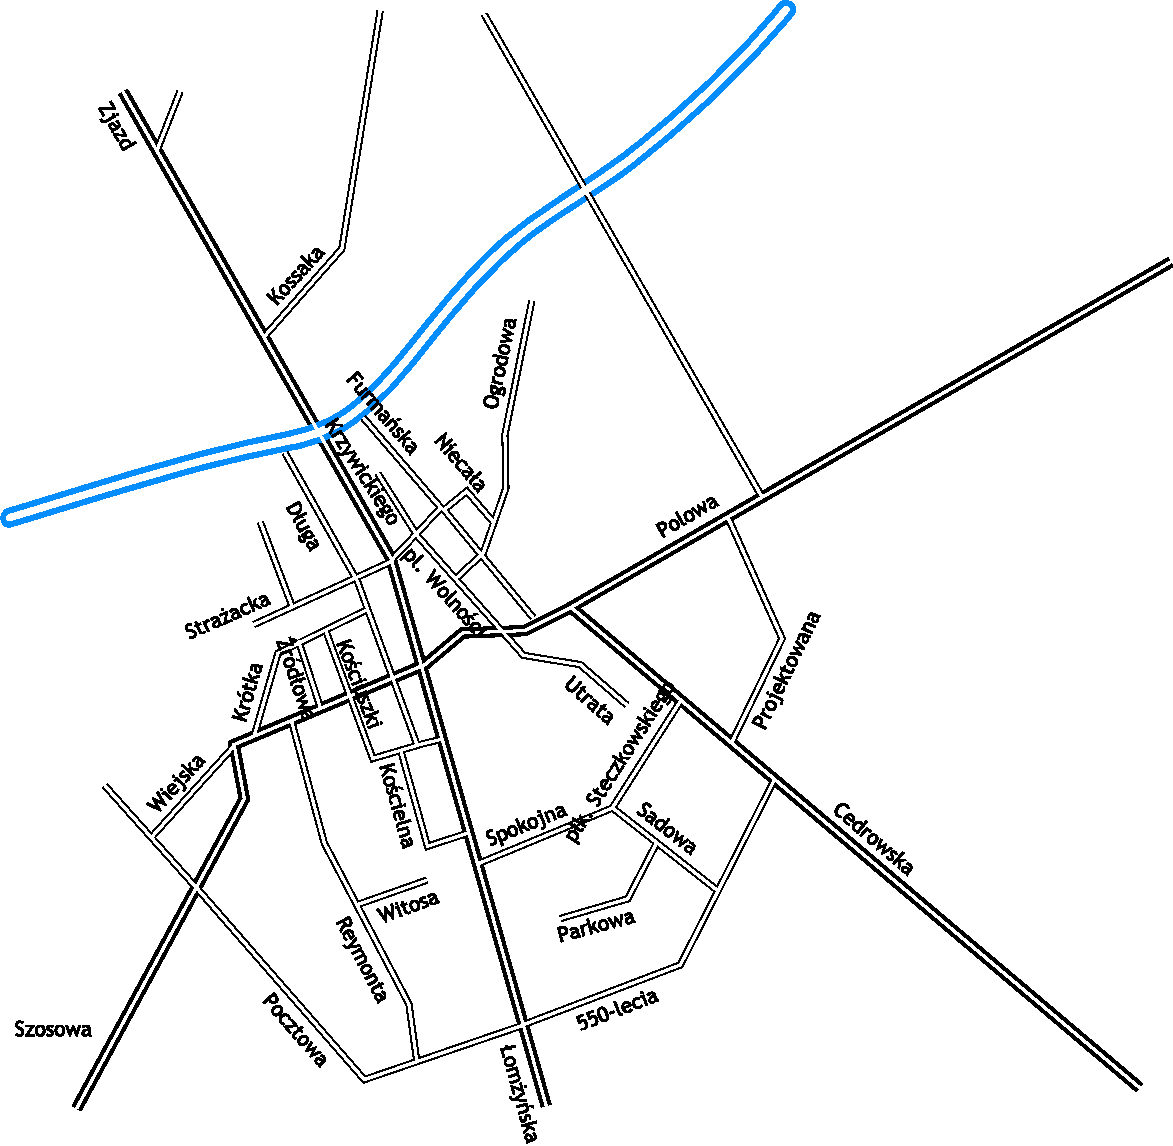
\includegraphics[width=.4\linewidth]{img/Anonymous-Map-of-Stawiska-in-Poland.pdf}
\end{tabular}

\section{重み付きグラフと表現}

辺に重みが付いたグラフ上の最短路問題を扱う.
たとえば,グラフの節点が都市,辺が移動手段,辺についたコストが所要時間
だとすれば,最短路問題は早く目的地に移動する問題と対応する.
コストが通行料だとすると,最も安く目的地につく手段を求めることと対応す
る.
辺に向きがある有向グラフの場合は,一方通行を表現可能である.なお,向き
がない場合は,有向グラフで逆向きのコストが常に等しい特殊ケースと考える
ことができる.

まずは,コストは非負であると仮定し(通行料を払うことはあっても報奨金をもらうことはない),後に一般の場合を考える.
この章の前半でのグラフの表現としては,
もっとも簡単な\textbf{隣接行列}を用い
る(\ref{section:adjacency-matrix}, \pccbook[pp.~90,~91]).隣接行列$K$の
$i,j$要素$K[i][j]$は,$i$から$j$に有向辺があればそのコスト,ない場合は
  $\infty$と表現する.


\section{全点対間最短路}

最短路問題を解くアルゴリズムには様々なものがあるが,
全ての節点間の最短路を求めるFloyd-Warshallを,まず覚えてくとよい(\pccbook[p.~97]).
見て分かるように\texttt{for}文を3つ重ねただけの,簡潔で実装が容易なア
ルゴリズムである.

\begin{algorithmic}[1]
\Procedure{Floyd-Warshall}{int K[][]}
\Comment{$i$から$j$への最短路のコスト$K[i][j]$を全て計算}
\Statex
\Comment{初期値は$K[i][j] = d_{ij}$ (i,j間に辺がある場合)}
\Statex
\Comment{または$K[i][j]=\infty$ (ない場合)}
\For{$\cemph{k}=1..N$}
\Comment{都市番号が$1..N$でない場合は,適宜変更すること}
\For{$i=1..N$}
\Comment{添字$\cemph{k}$を$i$や$j$と入れ替えると動かないので注意!}
\For{$j=1..N$}
\If{$K[i][j] > K[i][\cemph{k}]+K[\cemph{k}][j]$}\label{alg:floyd:relax}
\State $K[i][j] \gets K[i][\cemph{k}]+K[\cemph{k}][j]$;\label{alg:floyd:relax2}
\Comment{$\cemph{k}$を経由すると安い場合に更新}
\EndIf
\EndFor
\EndFor
\EndFor
\EndProcedure
\end{algorithmic}

動作の概略は以下の通り: 初期状態で$K[i][j]$は直接接続されている辺のみ
通る場合の移動コストを表す.アルゴリズム開始後,はじめに$k=1$のループ
が終了すると,$K[i][j]$は,$i-j$と移動する(直接接続されている辺を通る)か「$i-1-j$と順に移
動する」場合の最小値を表す.$k=2$のループが終了すると,$K[i][j]$は,
$i-j$または$i-1-j$または$i-2-j$または$i-1-2-j$または$i-2-1-j$と移動す
るルートの最小値を表す.一般に$k=a$のループが終了時点で$K[i][j]$は,経由
地として$1..a$までを通過可能なパスのコストの最小値を表す.

\begin{itembox}[l]{証明概略}
都市$a$までを経
由地に含む$i$から$j$の最短路(の一つ)を$D^a_{ij}$と表記する.$a\ge 2$の時
$D^a_{ij}$は,$a$を含む場合と含まない場合に分けられる.
含まない場合は,都市$a$に立ち寄っても遠回りになる場
合で,$D^{a-1}_{ij}$と同一である.含む場合は,$i$から$a$を経由して$j$
に到達する場合である.ここで,$i$から$a$までの移動や$a$から$j$までの移
動で$a$を通ることはない(ものだけ考えて良い).(各辺のコストが非負なので,
最短路の候補としては,各都市を最大1度だけ経由するパスのみを考えれば十分
である.) 従って$i$から$a$までの移動や$a$から$j$までの移
動の最短路はそれぞれ,$D^{a-1}_{ia}$と$D^{a-1}_{aj}$である.$a$に立ち
寄る場合と立ち寄らない場合を総合すると,$D^a_{ij}=\min(D^{a-1}_{ij}, D^{a-1}_{ia}+D^{a-1}_{aj})$となる.
\end{itembox}

\subsection{例題}

\begin{psbox}{A Reward for a Carpenter}{PC甲子園2005}
大工がどこかへ行って戻ってくる.(原文参照)
  
\aojid{0117}
\end{psbox}

\paragraph{入出力}
今回の入力はスペース区切りではなくカンマ(,)で区切られて与えられる.
このようなデータを読む場合には\texttt{scanf}を用いると楽ができ
る.

C++で使う場合の注意点としては,\texttt{cstdio}をincludeすることと,\texttt{scanf}を使う場合は\texttt{cin}は使わないこと.

\begin{cbox}
#include <iostream>
#include <cstdio>
using namespace std;
int N, M, A, B, C, D, x1, x2, y1, y2;
int main() {
    scanf("
    for (int i=0; i<M; ++i) {
        scanf("
        cerr << "read " << A << ' ' << B << ' ' << C << ' ' << D
             << endl;
        // A \dingright{} B がコストC
        // B \dingright{} A がコストD
    }
}
\end{cbox}


\paragraph{上限はいくつ?}

街の数は最大20であるから,行列$K$は十分に大きく設定する.
注意点としては,街の番号は1から20で与えられることと,C++の配列の先頭は
[0]であることである.今回は配列を大き目に確保して,必要な部分のみを使
う([0]は使わない)ことを勧める.


\begin{cbox}
int K[32][32];
\end{cbox}


プログラムとして実装するうえでは$\infty$として有限の数を用いる必要があ
る.
この数は,(1) どのような最短路よりも大きな数である必要がある.最短路の最大
値は全ての辺を通った場合で,各辺のコストの最大値と辺の数の積で見積もる
ことができる. (2) 2倍してもオーバーフローしないような,大きすぎない数である必要がある.(手順中\ref{alg:floyd:relax}, \ref{alg:floyd:relax2}行目で加算を行うため)

\begin{cbox}
const int inf = 1001001001;
\end{cbox}

多くの場合は10億程度の値を使っておけば十分である.(見積もりを越えないことを検算すること)

\paragraph{隣接行列の初期化}

入力を読み込んで隣接行列を設定する部分をまず実装しよう.
そして,隣接行列を表示する関数\texttt{void show()} を作成し,表示してみ
よう.表示部分は前回の関数を流用可能である.ただし,今回は0列目と0行目は使わないことに注意.

サンプル入力に対しては以下の出力となることを確認せよ.(infの代わりに具体的な数が書かれていても問題ない.また桁が揃っていなくても,自分が分かれば問題ない.)

\begin{alltt}
  inf    2    4    4  inf  inf
    2  inf  inf  inf    3  inf
    3  inf  inf    4  inf    1
    2  inf    2  inf  inf    1
  inf    2  inf  inf  inf    1
  inf  inf    2    1    2  inf
\end{alltt}

\paragraph{Floyd-Warshall}

続いて,最短路のコストを計算するFloyd-Warshallを実装する.
もっとも外側の\texttt{k}に関するループを行う度に,行列Kがどのように変
化するかを確認すると良い.

最初のループ(\texttt{k=1})終了後
\begin{alltt}
  inf    2    4    4  inf  inf
    2    4    6    6    3  inf
    3    5    7    4  inf    1
    2    4    2    6  inf    1
  inf    2  inf  inf  inf    1
  inf  inf    2    1    2  inf
\end{alltt}

最終状態
\begin{alltt}
    4    2    4    4    5    5
    2    4    6    5    3    4
    3    5    3    2    3    1
    2    4    2    2    3    1
    4    2    3    2    3    1
    3    4    2    1    2    2
\end{alltt}

\paragraph{回答の作成}

さて問題で要求されている回答は,
「大工の褒美」であり,それは
「柱の代金」-「殿様から大工が受け取ったお金」-「大工の町から山里までの最短コスト」-「山里から大工の町までの最短コスト」
である.
行列Kの参照と,適切な加減算で,回答を計算し出力せよ.

Acceptされたら他の方法でも解いてみよう.

\subsection{負の重みを持つ辺がある場合}

\begin{psbox}{Shortest Path - All Pairs Shortest Path}{AOJ}
  全頂点間の最短路を求めよ.ただし負の重みがありうる.

\aojid{GRL_1_C}
\end{psbox}

これまでは非負の重みを持つ辺のみを考えていたが,負の重みを持つ辺(\jindex{負辺}{ふへん})としてモ
デル化することが適切な場合もありうる.
たとえば,ある区間では通行料を払う代わりに小遣いをもらえるスゴロクなどを考えよう.
そのような場合に,最短路の概念はどう変化するだろうか?
コストが負でありうる場合は非負の場合に成り立つ性質のいくつかは成り立た
ないため,注意が必要である.特に,コストの総和が負である閉路,\jindex{負閉路}{ふへいろ}(negative weight cycle)がある場合には,
そこを回り続けるとコストは下がり続けるために最短路が定義できない.
始点から終点までの途上に負閉路が無ければ最短路は定義可能で,(正ではないかもしれないが)最小のコストが
定まる.

Floyd-Warshall法は幸い負閉路があっても動作し,終了時各点$i$について$K[i][i]<0$であるなら点$i$を含む閉路が存在する.
ただし実装にあたっては,辺の有無に注意を払う必要がある.たとえば上記の手順で\ref{alg:floyd:relax}行目の,
``\texttt{if} $K[i][j] > K[i][\cemph{k}]+K[\cemph{k}][j]$''という部分に,辺$ik$と$kj$の存在を条件に加えること.辺のコストが非負であれば存在しない辺のコストをinfとすることで辺の存在をついでに確認できたが,負辺が存在する場合は片方がinfでも足すと小さくなることがある.

\section{単一始点最短路} 

始点を一つ定めて始点から各点への最短路を求める問題は,全点対間で最小距離を求めるよりも効率的に解くことができる.
たとえば,往復のコストを求める場合は,往路と復路のそれぞれで単一始点最短路問題を2回解くと解が得られる.

\subsection{緩和 (relaxation)}

  \begin{center}
      \begin{tikzpicture}[node distance=25mm]
        \node[ccity,label={[label distance=3mm]270:$d_A=0$}] (A)              {$A$};
        \node[city,label={[label distance=3mm]270:$d_B=\infty$}] (B) [right of=A] {$B$};
        \node[city,label={[label distance=3mm]270:$d_C=\infty$}] (C) [right of=B] {$C$};
        \node[city,label={[label distance=3mm]270:$d_D=\infty$}] (D) [right of=C] {$D$};
        \path[->,draw=gray,thick] (A) edge node [above] {$10$} (B);
        \path[->,draw=gray,thick] (B) edge node [above] {$20$} (C);
        \path[->,draw=gray,thick] (C) edge node [above] {$5$} (D);
      \end{tikzpicture}
  \end{center}

はじめに,上のような単純なグラフを考え,Aを始点としてDまでの距離を求める問題を考える.

\textbf{定義:}
  $d[x]$ を $A$から$x$までの最短コストの\cemph{上限}とする.

初めに,
$d[A] = 0$ (AからAまではコストがかからない),
$d[B] = d[C] = d[D] = \infty$ (情報がないので$\infty$)と定める.

  \begin{center}
      \begin{tikzpicture}[node distance=25mm]
        \node[vcity,label={[label distance=3mm]270:$d_A=0$}] (A)              {$A$};
        \node[ccity,label={[label distance=3mm]270:$d_B=$\cemphp{$10$}}] (B) [right of=A] {$B$};
        \node[city,label={[label distance=3mm]270:$d_C=\infty$}] (C) [right of=B] {$C$};
        \node[city,label={[label distance=3mm]270:$d_D=\infty$}] (D) [right of=C] {$D$};
        \path[->,draw=ired,thick]  (A) edge node [above] {$10$} (B);
        \path[->,draw=gray,thick] (B) edge node [above] {$20$} (C);
        \path[->,draw=gray,thick] (C) edge node [above] {$5$} (D);
      \end{tikzpicture}
  \end{center}

\textbf{定義:緩和操作\\}
ある辺(s,t)とそのコスト,$w(s,t)$に対して,
$d[t] > d[s]+w(s,t)$である場合に,$d[t] = d[s]+w(s,t)$と$d[t]$を減らす
操作を\jindex{緩和}{かんわ}と呼ぶ.
$\delta[t]$を$t$までの真の最小距離とすると$\delta[t] \le \delta[s]+w(s,t)$
であるので,全ての節点で$\delta[n]\le d[n]$が保たれている状態で,この操作を行っても$\delta[t]\le d[t]$が保たれる.
辺ABに着目すると,$d[B] = min(d[B], d[A]+10) = 10$となり,
$d[B]$は$\infty$から$10$に変化する.

  \begin{center}
      \begin{tikzpicture}[node distance=25mm]
        \node[vcity,label={[label distance=3mm]270:$d_A=0$}] (A)              {$A$};
        \node[vcity,label={[label distance=3mm]270:$d_B=$\cemphp{$10$}}] (B) [right of=A] {$B$};
        \node[ccity,label={[label distance=3mm]270:$d_C=$\cemphp{$30$}}] (C) [right of=B] {$C$};
        \node[city,label={[label distance=3mm]270:$d_D=$$\infty$}] (D) [right of=C] {$D$};
        \path[->,draw=ired,thick]  (A) edge node [above] {$10$} (B);
        \path[->,draw=ired,thick]  (B) edge node [above] {$20$} (C);
        \path[->,draw=gray,thick] (C) edge node [above] {$5$} (D);
      \end{tikzpicture}
  \end{center}

  \begin{center}
      \begin{tikzpicture}[node distance=25mm]
        \node[vcity,label={[label distance=3mm]270:$d_A=0$}] (A)              {$A$};
        \node[vcity,label={[label distance=3mm]270:$d_B=$\textcolor{ired}{$10$}}] (B) [right of=A] {$B$};
        \node[vcity,label={[label distance=3mm]270:$d_C=$\textcolor{ired}{$30$}}] (C) [right of=B] {$C$};
        \node[ccity,label={[label distance=3mm]270:$d_D=$\cemphp{$35$}}] (D) [right of=C] {$D$};
        \path[->,draw=ired,thick] (A) edge node [above] {$10$} (B);
        \path[->,draw=ired,thick] (B) edge node [above] {$20$} (C);
        \path[->,draw=ired,thick] (C) edge node [above] {$5$} (D);
      \end{tikzpicture}
  \end{center}


同様に,
$d[C] = min(d[C], d[B]+20) = 30$,
$d[D] = min(d[D], d[C]+5) = 35$,
と進めるとDまでの距離が求まる.
$d$が変化しなくなるまで緩和を繰り返すと,真の最短コストが得られる.
どの順番に緩和を行うかで効率が異なる.
以下,頂点の集合を$V$, 有向辺の集合を$E$, 辺uvの重みを$w(u,v)$, 始点を$v_s$で表す.

\subsection{Bellman-Ford法}\label{section:BellmanFord}
(\pccbook[p.~95])

\begin{algorithmic}[1]
\Procedure{Bellman-Ford}{$V, E, w(u,v), v_s$}
\For{$v\in V$}
\State $d[v] \gets \infty$
\Comment{初期化: 頂点までの距離の上限は$\infty$}
\EndFor
\State $d[v_s] \gets 0$
\Comment{初期化: 始点までの距離は$0$}
\For{($|V|-1$)回}
\Comment{$|V|$回以上でも可}
\For{辺$(u,v) \in E$}\
\State \cemphp{$d[v] \gets \min(d[v], d[u]+w(u,v))$}
\Comment{緩和}
\EndFor
\EndFor
\EndProcedure
\end{algorithmic}

\begin{itemize}
\setlength{\itemsep}{0pt}
\item 緩和の順番は? -- 適当に一通り
\item いつまで続ける? 停まる? -- (頂点の数-1)回ずつ全ての辺について繰り返す
\item 本当に最短? -- 最短路の長さは最大$|V|-1$であることから証明 (負閉路がない場合)
\end{itemize}

\subsection{Dijkstra法}\label{section:dijkstra}
(\pccbook[p.~96])

\begin{algorithmic}[1]
\Procedure{Dijkstra}{$V, E, w(u,v), v_s$}
\For{$v\in V$}
\State $d[v] \gets \infty$
\Comment{初期化: 始点から各頂点までの距離の上限は$\infty$}
\EndFor
\State $d[v_s] \gets 0$
\Comment{初期化: 始点から始点までの距離は$0$}
\State $S\gets \emptyset$
\Comment{最短距離が確定した頂点の集合,最初は空}
\State $Q\gets V$ 
\Comment{最短距離が未確定の頂点の集合,最初は全て}
\While{$Q \ne \emptyset$}\label{alg:dijkstra:while}
\Comment{最短距離が未確定の頂点がなくなるまで繰り返し}
\State select $u\; s.t.\; $\cemphp{$\arg\min_{u\in Q} d[u]$}\label{alg:dijkstra:pop}
\Comment{「最短距離が未確定の頂点」で$d[u]$が最小の$u$を選択}
\State $S \gets S \cup \{u\}$, $Q \gets Q \setminus \{u\}$
\Comment{$u$までの最小距離は確定}
\For{$v \in Q\; s.t.\; (u,v) \in E$}
\State \cemphp{$d[v] \gets \min(d[v], d[u]+w(u,v))$}\label{alg:dijkstra:relax}
\Comment{緩和}
\EndFor
\EndWhile
\EndProcedure
\end{algorithmic}

\begin{itemize}
\setlength{\itemsep}{0pt}
\item 緩和の順番は? -- 最短コストが確定している頂点$u\in S$から出ている辺の
  行き先で最もコストが低い頂点$v$ (線形探索またはpriority queue等で管理)
\item いつまで続ける? 停まる? -- Qが空になると停止
\item 本当に最短? -- 背理法で証明 ($w$が非負の場合)
\end{itemize}


\subsection{手法の比較と負辺}
頂点の数を$V$とすると,
Floyd-Warshall 法は,for文の内側を見て分かる通り,$V^3$回の基本演算が行われる.
制限が1秒程度であるとすると,
$V=100$程度であれば余裕であるが,$V=1,000$になるともう難しい.
オーダ記法を用いると$O(V^3)$ となる.辺の数を$E$とすると,
Bellman-Ford法が$O(VE)$, Dijkstra 法が(実装によるが)
$O(V^2)$または$O(E \log V)$程度で,少し効率が良い.辺の数$E$は,完全グラフでは$V^2$程度,木
に近い場合は$V$程度なので,Bellman-Ford法や Dijkstra法がFloyd-Warshall 法よりどの程度早くなるかどうかはグラフの辺の数にも依存する.


\begin{pbox}{Single Source Shortest Path I}{AOJ}
都市$0$から全ての都市への最短路を求めよ.都市には$0$から$|V|-1$までの番号がついている.入力は,1行目に都市の数$|V|$,続く$|V|$行に各節点からの接続情報が与えられる.

詳しくは問題文を参照.
都市や辺の数が多いので,隣接行列ではなく\textbf{隣接リスト}で表現すると良い.

\aojid{GRL_1_A}  
\end{pbox}

\begin{tipsbox}{グラフの表現}
  この問題では都市の数が最大$100\,000$と多い.これを隣接行列で表そうとすると,
$(100\,000)^2$の要素数が必要となり,メモリ制限を確実に越える(試算せよ).
一方,辺の数は最大$500\,000$と$(100\,000)^2$より遥かに小さいので,辺毎に管理すると良い.
  Bellman-Ford法の場合は,問題文の指定通りに始点と終点を管理すれば十分
  である. Dijkstra法を用いる場合は,\texttt{vector}を用いて隣接リスト形式にすると都合が良い.
\end{tipsbox}

\paragraph{Bellman-Ford法で解いてみよう} サンプル入力1のグラフに対して,与えられた辺の順に処理を行った場合の動作は次のようになる.(この例では偶然全ての辺を一度づつ見るだけで最短距離が求まったが,グラフの形と辺の並び順に応じて一般には$|V|-1$回必要である.)
\begin{center}
\begin{tabular}{cc}
      \begin{tikzpicture}[node distance=20mm]
        \node[vcity,label={90:$d_0=0$}] (C0)              {$0$};
        \node[city,label={90:$d_1=\infty$}] (C1) [right of=C0] {$1$};
        \node[city,label={270:$d_2=\infty$}] (C2) [below of=C1] {$2$};
        \node[city,label={270:$d_3=\infty$}] (C3) [right of=C2] {$3$};
        \path[->,draw=gray,thick] (C0) edge node [above] {$1$} (C1);
        \path[->,draw=gray,thick] (C0) edge node [below] {$4$} (C2);
        \path[->,draw=gray,thick] (C1) edge node [left] {$2$} (C2);
        \path[->,draw=gray,thick] (C2) edge node [above] {$1$} (C3);
        \path[->,draw=gray,thick] (C1) edge node [above] {$5$} (C3);
      \end{tikzpicture}
&
      \begin{tikzpicture}[node distance=20mm]
        \node[vcity,label={90:$d_0=0$}] (C0)              {$0$};
        \node[city,label={90:$d_1=$\cemphp{$1$}}] (C1) [right of=C0] {$1$};
        \node[city,label={270:$d_2=\infty$}] (C2) [below of=C1] {$2$};
        \node[city,label={270:$d_3=\infty$}] (C3) [right of=C2] {$3$};
        \path[->,draw=ired,thick] (C0) edge node [above] {$1$} (C1);
        \path[->,draw=gray,thick] (C0) edge node [below] {$4$} (C2);
        \path[->,draw=gray,thick] (C1) edge node [left] {$2$} (C2);
        \path[->,draw=gray,thick] (C2) edge node [above] {$1$} (C3);
        \path[->,draw=gray,thick] (C1) edge node [above] {$5$} (C3);
      \end{tikzpicture}
\\
サンプル入力1の初期状態 & 辺\{0,1\}で緩和: $d_0+1=1 < \infty$\\
      \begin{tikzpicture}[node distance=20mm]
        \node[vcity,label={90:$d_0=0$}] (C0)              {$0$};
        \node[city,label={90:$d_1=1$}] (C1) [right of=C0] {$1$};
        \node[city,label={270:$d_2=$\cemphp{$4$}}] (C2) [below of=C1] {$2$};
        \node[city,label={270:$d_3=\infty$}] (C3) [right of=C2] {$3$};
        \path[->,draw=gray,thick] (C0) edge node [above] {$1$} (C1);
        \path[->,draw=ired,thick] (C0) edge node [below] {$4$} (C2);
        \path[->,draw=gray,thick] (C1) edge node [left] {$2$} (C2);
        \path[->,draw=gray,thick] (C2) edge node [above] {$1$} (C3);
        \path[->,draw=gray,thick] (C1) edge node [above] {$5$} (C3);
      \end{tikzpicture}
&
      \begin{tikzpicture}[node distance=20mm]
        \node[vcity,label={90:$d_0=0$}] (C0)              {$0$};
        \node[city,label={90:$d_1=1$}] (C1) [right of=C0] {$1$};
        \node[city,label={270:$d_2=$\cemphp{$3$}}] (C2) [below of=C1] {$2$};
        \node[city,label={270:$d_3=\infty$}] (C3) [right of=C2] {$3$};
        \path[->,draw=gray,thick] (C0) edge node [above] {$1$} (C1);
        \path[->,draw=gray,thick] (C0) edge node [below] {$4$} (C2);
        \path[->,draw=ired,thick] (C1) edge node [left] {$2$} (C2);
        \path[->,draw=gray,thick] (C2) edge node [above] {$1$} (C3);
        \path[->,draw=gray,thick] (C1) edge node [above] {$5$} (C3);
      \end{tikzpicture}
\\
辺\{0,2\}で緩和:$d_0+4=4 < \infty$ & 辺\{1,2\}で緩和: $d_1+2=3 < 4$\\
      \begin{tikzpicture}[node distance=20mm]
        \node[vcity,label={90:$d_0=0$}] (C0)              {$0$};
        \node[city,label={90:$d_1=1$}] (C1) [right of=C0] {$1$};
        \node[city,label={270:$d_2=3$}] (C2) [below of=C1] {$2$};
        \node[city,label={270:$d_3=$\cemphp{$4$}}] (C3) [right of=C2] {$3$};
        \path[->,draw=gray,thick] (C0) edge node [above] {$1$} (C1);
        \path[->,draw=gray,thick] (C0) edge node [below] {$4$} (C2);
        \path[->,draw=gray,thick] (C1) edge node [left] {$2$} (C2);
        \path[->,draw=ired,thick] (C2) edge node [above] {$1$} (C3);
        \path[->,draw=gray,thick] (C1) edge node [above] {$5$} (C3);
      \end{tikzpicture}
&
      \begin{tikzpicture}[node distance=20mm]
        \node[vcity,label={90:$d_0=0$}] (C0)              {$0$};
        \node[city,label={90:$d_1=1$}] (C1) [right of=C0] {$1$};
        \node[city,label={270:$d_2=3$}] (C2) [below of=C1] {$2$};
        \node[city,label={270:$d_3=4$}] (C3) [right of=C2] {$3$};
        \path[->,draw=gray,thick] (C0) edge node [above] {$1$} (C1);
        \path[->,draw=gray,thick] (C0) edge node [below] {$4$} (C2);
        \path[->,draw=gray,thick] (C1) edge node [left] {$2$} (C2);
        \path[->,draw=gray,thick] (C2) edge node [above] {$1$} (C3);
        \path[->,draw=ired,dotted] (C1) edge node [above] {$5$} (C3);
      \end{tikzpicture}\\
辺\{2,3\}で緩和: $d_2+1=4 < \infty$ & 辺\{1,3\}では更新が起こらない: $d_1+5=6 > 4$
\end{tabular}
\end{center}

\begin{cbox}
int V, E, R, S[500010], T[500010], D[500010]; // 問題で与えられる入力
int C[100010]; // 各頂点までの最短距離の上限
// 無限を表す定数を全頂点をたどる最大超に設定
const int Inf = 10000*100000+100;

int main() {
  cin >> V >> E >> R;
  for (int i=0; i<E; ++i) 
    cin >> S[i] >> T[i] >> D[i]; // 各辺を入力
  ... // Cを初期化: \texttt{C[R]}を0に,他を\texttt{Inf}に
  for (int t=0; t<V; ++t) { // V回繰り返す
    bool update = false;
    for (int i=0; i<E; ++i) {
      int s = S[i], t = T[i], d = D[i]; // i番目の辺の\texttt{s,t,d}に対して
      if (C[s] < Inf && ...) { // 辺\texttt{s,t}で緩和できるなら
	C[t] = ...// \texttt{C[t]}を更新;
	update = true; // 更新が起こったことを記録
      }
    }
    if (!update) break; // 辺を一巡して更新がなければ打ち切って良い
  }
  ... // 出力
}
\end{cbox}

\begin{pybox}
NV,NE,R = map(int,input().split()) # NXでXの個数を表した
Inf = 1001001001 # 全頂点を通るパスより大きな値
E = [tuple(map(int,input().split())) for _ in range(NE)]
# 初期化
D = [Inf for _ in range(NV)]
D[R] = 0
# メインのループ
for t in range(NV):
    update = 0
    for s,t,d in E:
        # try to decrease D[t] w.r.t. edge (s,t) with cost d, here
        # increment update if D[t] was changed (decreased)
    if update == 0:
        break
for v in range(NV):
    print(D[v] if D[v] != Inf else "INF")  
\end{pybox}


\paragraph{Dijkstra法で解いてみよう}
Dijkstra法(\ref{section:dijkstra}節)で解く場合は,優先度つきキュー
(\textbf{priority queue}, \ref{section:priority-queue}章参照)を使うと便利である.
C++には標準ライブラリとして\texttt{priority\_queue}があるのでそれを使うと良い.
始点からの距離と都市のペア\texttt{pair<int,int>}を管理し,手順\ref{alg:dijkstra:pop}行目で,
距離の近い順に都市を取り出す.そのために,手順\ref{alg:dijkstra:relax}行目で更新が行われた頂
点を優先度つきキューに\texttt{push}する.本来はキュー内部にある頂点の
距離を減らすことが出来ると効率が良いが,多くの標準ライブラリの実装では
難しい.代わりに重複して\texttt{push}し,二度目以降に取り出した頂点は無視する.
注意点として,C++の標準ライブラリの\textbf{priority\_queue}は\textbf{大きい順}に要素を取り出すので,比較関数を指定して動作を変更するか,距離の符号を反転させて与えるような工夫が必要となる.

上記の方針で実装したDijkstra法の動作例を,以下に示す.優先度つきキュー$P$は,$\langle$~始点からの距離,~頂点番号~$\rangle$のペアを要素として持ち,距離の小さい順に,先頭要素(左端)が取り出されるとする.図のグラフ1つが手順\ref{alg:dijkstra:while}行目からのループの1回の実行に対応する.
\begin{center}
\begin{tabular}{cc}
      \begin{tikzpicture}[node distance=20mm]
        \node[ccity,label={90:$d_0=0$}] (C0)              {$0$};
        \node[city,label={90:$d_1=\infty$}] (C1) [right of=C0] {$1$};
        \node[city,label={270:$d_2=\infty$}] (C2) [below of=C1] {$2$};
        \node[city,label={270:$d_3=\infty$}] (C3) [right of=C2] {$3$};
        \path[->,draw=gray,thick] (C0) edge node [above] {$1$} (C1);
        \path[->,draw=gray,thick] (C0) edge node [below] {$4$} (C2);
        \path[->,draw=gray,thick] (C1) edge node [left] {$2$} (C2);
        \path[->,draw=gray,thick] (C2) edge node [above] {$1$} (C3);
        \path[->,draw=gray,thick] (C1) edge node [above] {$5$} (C3);
      \end{tikzpicture}
&
      \begin{tikzpicture}[node distance=20mm]
        \node[vcity,label={90:$d_0=0$}] (C0)              {$0$};
        \node[ccity,label={90:$d_1=$\cemphp{$1$}}] (C1) [right of=C0] {$1$};
        \node[ccity,label={270:$d_2=$\cemphp{$4$}}] (C2) [below of=C1] {$2$};
        \node[city,label={270:$d_3=\infty$}] (C3) [right of=C2] {$3$};
        \path[->,draw=ired,thick] (C0) edge node [above] {$1$} (C1);
        \path[->,draw=ired,thick] (C0) edge node [below] {$4$} (C2);
        \path[->,draw=gray,thick] (C1) edge node [left] {$2$} (C2);
        \path[->,draw=gray,thick] (C2) edge node [above] {$1$} (C3);
        \path[->,draw=gray,thick] (C1) edge node [above] {$5$} (C3);
      \end{tikzpicture}
\\
初期状態 &$\langle 0, 0\rangle$を取り出し頂点0を確定,頂点1, 2を緩和\\
$P=(\langle 0, 0\rangle)$ &  $P=(\langle 1, 1\rangle, \langle 4, 2\rangle)$ \\
      \begin{tikzpicture}[node distance=20mm]
        \node[vcity,label={90:$d_0=0$}] (C0)              {$0$};
        \node[vcity,label={90:$d_1=1$}] (C1) [right of=C0] {$1$};
        \node[ccity,label={270:$d_2=$\cemphp{$3$}}] (C2) [below of=C1] {$2$};
        \node[ccity,label={270:$d_3=$\cemphp{$6$}}] (C3) [right of=C2] {$3$};
        \path[->,draw=gray,thick] (C0) edge node [above] {$1$} (C1);
        \path[->,draw=gray,thick] (C0) edge node [below] {$4$} (C2);
        \path[->,draw=ired,thick] (C1) edge node [left] {$2$} (C2);
        \path[->,draw=gray,thick] (C2) edge node [above] {$1$} (C3);
        \path[->,draw=ired,thick] (C1) edge node [above] {$5$} (C3);
      \end{tikzpicture}
&
      \begin{tikzpicture}[node distance=20mm]
        \node[vcity,label={90:$d_0=0$}] (C0)              {$0$};
        \node[vcity,label={90:$d_1=1$}] (C1) [right of=C0] {$1$};
        \node[vcity,label={270:$d_2=3$}] (C2) [below of=C1] {$2$};
        \node[ccity,label={270:$d_3=$\cemphp{$4$}}] (C3) [right of=C2] {$3$};
        \path[->,draw=gray,thick] (C0) edge node [above] {$1$} (C1);
        \path[->,draw=gray,thick] (C0) edge node [below] {$4$} (C2);
        \path[->,draw=gray,thick] (C1) edge node [left] {$2$} (C2);
        \path[->,draw=ired,thick] (C2) edge node [above] {$1$} (C3);
        \path[->,draw=gray,thick] (C1) edge node [above] {$5$} (C3);
      \end{tikzpicture}
\\
頂点1を確定して頂点2, 3を緩和 & 頂点2を確定して頂点3を緩和 \\
$P=(\langle 3, 2\rangle, \langle 4, 2\rangle, \langle 6, 3\rangle)$ 
&$P=(\langle 4, 2\rangle, \langle 4, 3\rangle, \langle 6, 3\rangle)$
\\
      \begin{tikzpicture}[node distance=20mm]
        \node[vcity,label={90:$d_0=0$}] (C0)              {$0$};
        \node[vcity,label={90:$d_1=1$}] (C1) [right of=C0] {$1$};
        \node[vcity,label={270:$d_2=3$}] (C2) [below of=C1] {$2$};
        \node[ccity,label={270:$d_3=4$}] (C3) [right of=C2] {$3$};
        \path[->,draw=gray,thick] (C0) edge node [above] {$1$} (C1);
        \path[->,draw=gray,thick] (C0) edge node [below] {$4$} (C2);
        \path[->,draw=gray,thick] (C1) edge node [left] {$2$} (C2);
        \path[->,draw=gray,thick] (C2) edge node [above] {$1$} (C3);
        \path[->,draw=gray,thick] (C1) edge node [above] {$5$} (C3);
      \end{tikzpicture}
&
      \begin{tikzpicture}[node distance=20mm]
        \node[vcity,label={90:$d_0=0$}] (C0)              {$0$};
        \node[vcity,label={90:$d_1=1$}] (C1) [right of=C0] {$1$};
        \node[vcity,label={270:$d_2=3$}] (C2) [below of=C1] {$2$};
        \node[vcity,label={270:$d_3=4$}] (C3) [right of=C2] {$3$};
        \path[->,draw=gray,thick] (C0) edge node [above] {$1$} (C1);
        \path[->,draw=gray,thick] (C0) edge node [below] {$4$} (C2);
        \path[->,draw=gray,thick] (C1) edge node [left] {$2$} (C2);
        \path[->,draw=gray,thick] (C2) edge node [above] {$1$} (C3);
        \path[->,draw=gray,thick] (C1) edge node [above] {$5$} (C3);
      \end{tikzpicture}
\\
頂点2は既に確定しているので$\langle 4, 2\rangle$は無視 & $\langle 4, 3\rangle$を取り出し頂点3が距離4で確定\\
$P=(\langle 4, 3\rangle, \langle 6, 3\rangle)$&$P=(\langle 6, 3\rangle)$
\end{tabular}
\end{center}


\begin{pbox}{Single Source Shortest Path II}{AOJ}
重みが負の辺がある場合に,都市$0$から全ての都市への最短路を求めよ.
詳しくは問題文を参照.

\aojid{GRL_1_B}  
\end{pbox}

重みが負の辺がある場合は,Dijkstra法は正しく動作しない. Bellman-Ford法は最短路が定義される場合には正しい解を発見可能で,負閉路の存在は頂点の個数$|V|$回目の更新を試みて成功するかどうかで確認できる.

\begin{pbox}{Wormholes}{USACO 2006 December Gold}
  ワームホールを通じて過去に戻れるルートを探す.出発地はどこを選んでも良いので,その場所の過去の時刻に戻れれば良い.

\url{http://poj.org/problem?id=3259}
\end{pbox}

\section{練習問題}

\begin{pbox}{Railway Connection$\star$}{国内予選2012}
最も安い運賃の経路を求める

\aojid{1182}
\end{pbox}

ヒント: 距離と料金の二つの観点があるので,それぞれ対応する.(つづきは白文字で)
\textcolor{white}{(1) 各会社について,その会社の路線のみ使う場合の,全駅間の距離の最短路を求める.求めた距離を料金に変換する.(2) 上記で求めた料金を元に,最安の意味での最短路を求める.}

\begin{pbox}{崖登り$\star$}{国内予選2007}
崖を登る最短の時間を求める

\aojid{1150}
\end{pbox}

\begin{pbox}{Magical Dungeon$\star$}{冬合宿2008}
  ヒットポイントHを持つ勇者が部屋Sから移動して部屋Tに到着した瞬間にモ
  ンスターと戦う.最大いくつのヒットポイントで戦闘を迎えられるか?
通路には正負の数が割り当てられていて,正ならヒットポイントを回復し,負なら失う.ヒットポイントが0以下になるような移動はできない.ヒットポイントがHを超えるような移動は可能ではあるが,ヒットポイントは最大Hまでしか回復しない.

\aojid{2124}

問題とデータセット: \url{http://acm-icpc.aitea.net/index.php?2007\%2FPractice\%2F\%E5\%86\%AC\%E5\%90\%88\%E5\%AE\%BF\%2F\%E5\%95\%8F\%E9\%A1\%8C\%E6\%96\%87\%E3\%81\%A8\%E3\%83\%87\%E3\%83\%BC\%E3\%82\%BF\%E3\%82\%BB\%E3\%83\%83\%E3\%83\%88} (day3, C)
\end{pbox}

注: 負の閉路を\textcolor{white}{ぐるぐるまわって回復してから戦うようなケースを考える必要がある.
Bellman-Ford法の応用で解くことができるが,Hが大きいケースを効率的に対処するには,}少し工夫が必要.

\begin{pbox}{壊れたドア$\star$}{国内予選2011}
どこかのドアが壊れている条件で,最も都合が悪い場所で壊れたドアが見つかっ
た時点からの迂回を考慮した最短路を求める.

\aojid{1178}
\end{pbox}

\begin{pbox}{The Most Powerful Spell$\star\star$}{国内予選2010}
作成可能な中で,辞書順で最も早い呪文を求める.

\aojid{1169}
\end{pbox}

\begin{pbox}{Sums$\star$}{10th Polish Olympiad in Informatics}
整数の集合Aが与えられる.質問として与えられる数が,Aの要素の和で表せる
かどうかを答えよ.(正確な条件は原文参照)

補足: $a_0 \cdot n$は上限まで大きくならないと想定して良い.

\url{https://szkopul.edu.pl/problemset/problem/4CirgBfxbj9tIAS2C7DWCCd7/site/}
\end{pbox}
 % Commented out: Included file


\part{Topics}

%\chapter{平面の幾何}

\section{概要: 点の表現と演算}

\begin{itembox}[l]{概要}
さまざまな状況で計算機で図形的問題を扱う機会に出会う.ここでは幾何の
問題を扱う基本を紹介したい(詳しく学ぶには専門の授業を受講されたい).たと
えば,平行や図形の内外などよく馴染んだ概念を,「符号付き三角形の面積」
という道具で,表してみよう.人間には簡単な図形の概念でも,プログラムと
して記述する場合は直感的ではない方法が適する場合がある.また浮動小数
(\texttt{double}など)を扱うので,誤差に注意する必要も生ずる.
\end{itembox}

平面上の点をCやC++で表現する場合には,たとえば構造体を用いる方法がある(\pcaojbook[pp.~365--(16章)]).この資料では,少し楽をして
以下のように複素数で表現する

\subsection{複素数による点の表現}

\paragraph{C++の複素数による表現}
C++では標準ライブラリの\eindex{complex}型を用いる.(実部\texttt{real()}を\texttt{x}に,虚部\texttt{imag()}を\texttt{y}に対応させる):
\begin{center}
\begin{tikzpicture}
\coordinate (O) at (0,0);
\coordinate (P) at (-2,1);
\coordinate (Q) at (3,-1);
\draw [step=1cm,dotted] (-4.2,-1.2) grid (4.2,1.9);
\draw [->,ultra thick] (-4.5,0) -- (4.9,0);
\draw [->,ultra thick] (0,-1.3) -- (0,2.0);
\node [above] at (4.5,0) {X};
\node [right] at (0,1.8) {Y};
\draw [fill=black] (O) circle (2pt);
\node [below left] at (0,0) {O};
\draw [fill=black] (P) circle (3pt);
\node [above left] at (P) {P (-2,1)};
\draw [fill=black] (Q) circle (3pt);
\node [above right] at (Q) {Q};
\draw [->,thick,dashed] (P) -- (2.9,-0.9);
\end{tikzpicture}
\end{center}

\begin{cbox}[emph={complex,real,imag}]
#include <complex>
#include <cmath>
typedef complex<double> xy_t;
xy_t P(-2, 1), Q; // 初期化
cout << P << endl; // (debug用)表示
cout << P.real() << endl; // x 座標
cout << P.imag() << endl; // y 座標
Q = P + xy_t(5, -2); // 点Qは点Pを(5,-2)だけ平行移動した位置とする
Q *= xy_t(cos(a), sin(a)); // 点Qを原点を中心にa(ラジアン)だけ回転
cout << abs(P) << endl; // ベクトルOPの長さ
cout << norm(P) << endl; // \texttt{norm(P) = abs(P)}${}^2$
\end{cbox}

\paragraph{Cの複素数による表現} この資料では,Cの使用は非推奨であるが,後述する注意事項のために,一応掲載する.

C (gccまたはC99)の場合:
\begin{purecbox}[emph={complex,creal,cimag}]
#include <complex.h>
#include <math.h>
complex a = 0.0 + 1.0I; // 初期化
complex b = cos(3.14/4) + sin(3.14/4)*I;
printf("
a *= b; // 乗算
printf("
\end{purecbox}

\begin{debugbox}{乗算記号の入れ忘れに注意}
  数の\texttt{5}と変数\texttt{k}の積を求める場合は,\texttt{5*k}と書き,\texttt{5k}と書くとコンパイルエラーになる.ところが,文字\texttt{i,j,I,J}に関しては,\texttt{5j}などの表記が上記の虚数と解釈され,コンパイルエラーにはならない.\texttt{cout}に表示すると,\texttt{bool}にキャストされて\texttt{1}と表示される.知らないと見つけにくい,と思われる.
\end{debugbox}

\medskip

\paragraph{Pythonの複素数による表現} Python3においても複素数\texttt{complex}をほぼ同様に利用可能である.詳細は\texttt{help(complex)}や\texttt{help(cmath)}で確認のこと.
\begin{pybox}[emph={real,imag,complex}]
import cmath
import math
P = complex(-2,1) # \texttt{(-2+1j)}も可
print(P)
print(P.real)     # 実部
print(P.imag)     # 虚部
Q = P + complex(5,-2)     # 平行移動
Q *= complex(math.cos(a), math.sin(a))     # 回転
print(abs(P))     # 長さ
\end{pybox}
\subsection{よく使う演算}

\begin{center}
\begin{tabular}{c@{\hspace{5em}}c}
\begin{tikzpicture}
\coordinate (O) at (0,0);
\coordinate (A) at (3,1);
\coordinate (B) at (1,2);
\coordinate (BcosT) at (1.45,0.5);
\draw [step=1cm,dotted] (-0.5,-0.5) grid (3.9,3.9);
\draw [->,ultra thick] (-0.5,0) -- (4,0);
\draw [->,ultra thick] (0,-0.5) -- (0,4);
\node [above] at (4,0) {X};
\node [right] at (0,4) {Y};
\draw [fill=black] (A) circle (3pt);
\node [above right] at (A) {$a$};
\draw [fill=black] (B) circle (3pt);
\node [above left] at (B) {$b$};
\draw [] (BcosT) circle (3pt);
\node [below right] at (BcosT) {$b\cos\theta$};
\draw [->,thick] (O) -- (2.9,0.9);
\draw [->,thick] (O) -- (0.9,1.9);
\draw [->,thick] (0.6,0.25) arc (30:60:0.8);
\draw [thick,dashed] (B) -- (BcosT);
\node at (0.7,0.7) {$\theta$};
\end{tikzpicture}
&
\begin{tikzpicture}
\coordinate (O) at (0,0);
\coordinate (A) at (2,1);
\coordinate (B) at (1,2);
\coordinate (AB) at (3,3);
\draw [color=white,fill=gray!25!] (O) -- (A) -- (AB) -- (B) -- cycle;
\draw [step=1cm,dotted] (-0.5,-0.5) grid (3.9,3.9);
\draw [->,ultra thick] (-0.5,0) -- (4,0);
\draw [->,ultra thick] (0,-0.5) -- (0,4);
\node [above] at (4,0) {X};
\node [right] at (0,4) {Y};
\draw [fill=black] (A) circle (3pt);
\node [right] at (A) {$a$};
\draw [fill=black] (B) circle (3pt);
\node [above left] at (B) {$b$};
\draw [] (AB) circle (3pt);
\node [above right] at (AB) {$a+b$};
\draw [->,thick] (O) -- (1.9,0.9);
\draw [->,thick] (O) -- (0.9,1.9);
\draw [->,thick] (1.5,0.75) arc (30:60:1.9);
\draw [->,thick,dashed] (A) -- (2.9,2.8);
\draw [->,thick,dashed] (B) -- (2.8,2.9);
\end{tikzpicture}
\\
(1) 内積: $|a||b|\cos\theta$ & (2) クロス(外)積: 網掛け部分の符号付き面積
\end{tabular}
\end{center}

\begin{cbox}[emph={cross_product,dot_product,projection}]
// 図(1) 内積: a.x*b.x +a.y*b.y
double dot_product(xy_t a, xy_t b) { return (conj(a)*b).real(); }
// 図(2) クロス(外)積, ベクトルa,bが作る\textcolor{ired}{三角形の符号付き面積}の二倍: a.x*b.y - b.x*a.y
double cross_product(xy_t a, xy_t b) { return (conj(a)*b).imag(); }
// (対応図なし) 投影 原点とbを結ぶ直線に点pを投影
xy_t projection(xy_t p, xy_t b) { return b*dot_product(p,b)/norm(b); }
\end{cbox}

三角形の\jindex{符号付き面積}{ふごうつきめんせき}の紹介が本章前半の主要なテーマである.これは原点と点a,bが作る三角形の面積を,符号付きで求める.符号は,原点と点a,bがこの順で反時計回りの位置関係にある場合に正,時計回りの場合に負となる.面積だけでなく,これから見るように向きの判定にも用いられる.

内積は,直線上に点を投影する際に便利である.

\begin{pybox}[emph={cross_product,dot_product,projection,norm}]
def norm(c):
    a = abs(c)
    return a*a
def dot_product(a, b):
    return (a.conjugate()*b).real
def cross_product(a,b):
    return (a.conjugate()*b).imag
def projection(p, b):
    return b*dot_product(p,b)/norm(b)  
\end{pybox}

\section{三角形の符号付き面積の利用}

\subsection{多角形の面積}
\begin{psbox}{Area of Polygon}{PC甲子園2005}
  凸多角形の面積を求めよ.

注1: 問題文中にはヘロンの公式が書いてあるが,下記の符号付き三角形で解くこと.(あとで凸でない多角形の面積に応用するため)

注2: 頂点列は順に与えられるが,時計回りか反搬時計回りかは指定がないため,最後に絶対値をとる.

\aojid{0079}
\end{psbox}

\begin{center}
\begin{tikzpicture}
\coordinate (O) at (0,0);
\coordinate (A) at (2,1);
\coordinate (B) at (1,2);
\coordinate (P0) at (5,1);
\coordinate (P1) at (7,2);
\coordinate (P2) at (6,3);
\draw [color=white,fill=gray!20!] (P0) -- (P1) -- (P2) -- cycle;
\draw [] (P0) -- (P1) -- (P2) -- (5,3) -- (4,2) -- cycle;
\draw [step=1cm,dotted] (-0.5,-0.5) grid (7.9,3.9);
\draw [->,ultra thick] (-0.5,0) -- (8,0);
\draw [->,ultra thick] (0,-0.5) -- (0,4);
\node [above] at (8,0) {X};
\node [right] at (0,4) {Y};
\node [above right] at (A) {$a=p_1-p_0$};
\node [above] at (B) {$b=p_2-p_0$};
\draw [->,thick] (O) -- (1.9,0.9);
\draw [->,thick] (O) -- (0.9,1.9);
\draw [->,thick] (1.5,0.75) arc (30:60:1.9);
\draw [thick,dashed] (5,1) -- (6,3);
\draw [thick,dashed] (5,1) -- (5,3);
\node [below] at (P0) {$p_0$};
\node [right] at (P1) {$p_1$};
\node [above] at (P2) {$p_2$};
\draw [dotted] (A) -- (P1);
\draw [dotted] (B) -- (P2);
\draw [dotted] (O) -- (P0);
\end{tikzpicture}
\end{center}

(単純)多角形は三角形に分解できるので,三角形の面積が計算できれば,多角形の面
積が計算できる.特に凸多角形の場合は,一つの頂点とその頂点を含まない辺
が構成する三角形で綺麗に分割できる.

\begin{cbox}
xy_t P[110];
int main() {
  // 入力例 読み込んだ点の個数をNとする
  int N=0;
  double x, y;
  while (~scanf("
    P[N++] = xy_t(x,y);
  }
  // 面積計算
  double sum = 0.0;
  for (int i=0; i+2<N; ++i) {
    xy_t a=P[0], b=P[i+1], c=P[i+2];
    sum += ... // 三角形 abc の面積を加算
  }
  printf("
}
\end{cbox}

\begin{tipsbox}{scanfで入力が続く限り読む方法}
入力行を読める限り読むために,サンプルコード中では\texttt{while (\~{}scanf("\%lf,\%lf", \&x, \&y))}というループを採用した.これは,短い(しかし汎用性の低い)書き方で,\texttt{\~{}EOF}が0になる環境でのみ使用可能である.
\end{tipsbox}

\begin{pybox}
P = [] # 頂点列
try:
    while True:
        x,y = map(float,input().split(','))
        P.append(complex(x,y))
except EOFError:
    pass
N = len(P) # 頂点の個数
total = 0.0
for i in range(1,N-1):
    a,b,c = P[0],P[i],P[i+1]
    total += .. // 三角形 abc の面積を加算
print("
\end{pybox}

\begin{tipsbox}{Python3で入力が続く限り読む方法}
\texttt{input()}を試みて入力が終わっていた場合,Pythonでは\texttt{EOFError}という例外が発生するので,あらかじめ\texttt{try}で囲み\texttt{except}で検知する.例外が発生すると\texttt{input()}の書かれていた\texttt{while}ループを脱出して,外側の\texttt{except}ブロックが実行される(この場合は\texttt{pass}で,何もせずに次の行に移る).
\end{tipsbox}

\begin{psbox}{Polygon - Area}{AOJ}
多角形の面積を計算する.凸とは限らないが,頂点は反時計回りで与えられる.  

\aojid{CGL_3_A}

(類題: Area of Polygons (国内予選1998) \aojid{1100} 頂点が与えられる向きのみ異なる)
\end{psbox}
凸でない単純多角形に対して,先ほどと同様の分割を行うと三角形に重なりが生ずるが,ここで符号付き面積の符号も含めて合計すると,(不思議なことに)正しい面積を得られる.多角形の頂点は反時計回りに順に与えられている必要がある.なお分割の中心として$p_0$を使ったが,任意の点(たとえば原点)と各辺の作る三角形を考えても良い.

\begin{center}
  \begin{tabular}{ccc}
\begin{tikzpicture}[scale=0.8]
\coordinate (P0) at (2.5,1.5);
\coordinate (P1) at (5,1);
\coordinate (P2) at (3,3);
\coordinate (P3) at (6,3);
\coordinate (P4) at (2,4);
\draw [color=iblue,fill=gray!20!,thick,dashed] (P0) -- (P1) -- (P2) -- cycle;
\draw [] (P0) -- (P1) -- (P2) -- (P3) -- (P4) -- cycle;
\node [below] at (P0) {$p_0$};
\node [right] at (P1) {$p_1$};
\node [above] at (P2) {$p_2$};
\node [right] at (P3) {$p_3$};
\node [left] at (P4) {$p_4$};
\draw [->,ultra thick,dotted,color=iblue] ($(P0)+(1.0,0.6)$) ++(-60:0.5) arc (-60:210:0.5);
1\end{tikzpicture}
&
\begin{tikzpicture}[scale=0.8]
\coordinate (P0) at (2.5,1.5);
\coordinate (P1) at (5,1);
\coordinate (P2) at (3,3);
\coordinate (P3) at (6,3);
\coordinate (P4) at (2,4);
\draw [color=iblue,fill=gray!20!,thick,dashed] (P0) -- (P2) -- (P3) -- cycle;
\draw [] (P0) -- (P1) -- (P2) -- (P3) -- (P4) -- cycle;
\node [below] at (P0) {$p_0$};
\node [right] at (P1) {$p_1$};
\node [above] at (P2) {$p_2$};
\node [right] at (P3) {$p_3$};
\node [left] at (P4) {$p_4$};
\draw [->,ultra thick,dotted,color=ired] ($(P0)+(1.6,0.7)$) ++(235:0.5) arc (235:-30:0.5);
\end{tikzpicture}
&
\begin{tikzpicture}[scale=0.8]
\coordinate (P0) at (2.5,1.5);
\coordinate (P1) at (5,1);
\coordinate (P2) at (3,3);
\coordinate (P3) at (6,3);
\coordinate (P4) at (2,4);
\draw [color=iblue,fill=gray!20!,thick,dashed] (P0) -- (P3) -- (P4) -- cycle;
\draw [] (P0) -- (P1) -- (P2) -- (P3) -- (P4) -- cycle;
\node [below] at (P0) {$p_0$};
\node [right] at (P1) {$p_1$};
\node [right] at (P3) {$p_3$};
\node [left] at (P4) {$p_4$};
\draw [->,ultra thick,dotted,color=iblue] ($(P0)+(0.6,1.3)$) ++(-60:0.5) arc (-60:210:0.5);
\end{tikzpicture}
\\
$p_0p_1p_2$ (sgn: +)
&
$p_0p_2p_3$ (sgn: -)
&
$p_0p_3p_4$ (sgn: +)
  \end{tabular}
\end{center}


  
\subsection{平行の判定}

\begin{psbox}{Parallelism}{PC甲子園2003}
概要: A = (x1, y1), B = (x2, y2), C = (x3, y3), D = (x4, y4) の異なる4つの座標点が与えられたとき,直線 AB と CD が平行かどうかを判定せよ.

点の座標は小数点以下最大 5 桁までの数字を含む実数で与えられる(この情報を数値誤差の推定に用いる).

\aojid{0021}
\end{psbox}

回答方針: ベクトルABとベクトルCDからなる三角形が面積を持つかどうかを判定すれば良い

\begin{cbox}[emph={eps}]
const double eps = 1e-11;
double x[4], y[4];
int N;
int main() {
    cin >> N; // 問題数
    for (int t=0; t<N; ++t) {
        for (int i=0; i<4; ++i) 
            cin >> x[i] >> y[i]; // x0,y0..x3,y3
        xy_t a[2] = {
            xy_t(x[0],y[0]) - xy_t(x[1],y[1]), 
            xy_t(x[2],y[2]) - xy_t(x[3],y[3])
        };
        bool p = abs(a[0]とa[1]の符号付き面積) < eps;
        cout << (p ? "YES" : "NO") << endl;
    }
}
\end{cbox}

補足: 向きや角度の判定には,\texttt{sin}や\texttt{arg}などのライブラリ
関数を用いることもできるが,計算誤差の観点から可能な限り符号付き面積で
計算するほうが良い.たとえば三角関数の汎用的な実装方法ではTaylor展開が用いられる.
\footnote{参考: FreeBSDの実装 \url{https://svnweb.freebsd.org/base/release/10.1.0/lib/msun/src/k_cos.c?view=markup}}

\begin{pybox}
N = int(input())
for _ in range(N):
    P = list(map(float,input().split()))
    a, b, c, d = [complex(P[i*2],P[i*2+1]) for i in range(4)]
    parallel = ... # abとcdが並行かを表す真偽値を計算
    print("YES" if parallel else "NO")
\end{pybox}

\begin{debugbox}{動作確認}
  この問題はサンプル入出力例が少なく,またジャッジデータも非公開である.そのため,自分でテストデータを試すと良い.たとえば,長い線,短い線,面積の符号の正負などが,確認すべき例である.

たとえば,以下の例は全て ``NO''である.
  \begin{terminal}
-0.00001 0 0.00001 0 -0.0001 0 0.00001 0.00001
-100 100 100 100 -100 100 100 99.99999
  \end{terminal}
\end{debugbox}

\medskip

\paragraph{数値誤差の取り扱い$\star$}
\texttt{double}などの浮動小数を用いる時には,$\frac{1}{2}$の冪乗の和で
表される数値以外は,必然的に誤差を含む(\ref{section:floating-point-numbers}章も参照).この問題での入力は,絶対値が100以下かつ各値
は小数点以下最大5桁までの数値と明示されているの
で,$10^5$倍して整数(\texttt{long long})で扱えば誤差の影響を避けることができる.
あるいは,サンプルコードの\texttt{eps}のように,誤差の範囲を予測する方法もある.
二つのベクトル$(a,b)$と$(c,d)$にそれぞれの要素に誤差が加わった時に,
(1)平行の場合に$|ad-bc|$の取る最大値(誤差がなければ$0$)と,(2)平行でない場合に$|ad-bc|$の取る最小値を比較して,(1)$<$閾値$<$(2)となるよう閾値をとる.
粗く見積もると(1)は最大
$(4\cdot100)\cdot(100\cdot2^{-54})\approx2.2\cdot10^{-12}$程度
($100\cdot2^{-54}$は100までの数を\texttt{double}で表した時の表現誤差,400は
$|(a+\varepsilon)(d+\varepsilon)-(b+\varepsilon)(c+\varepsilon)|$を展開した時の
$\varepsilon$にかかる係数の見積もり), 
(2)は$10^{-10}$程度(入力が表現可能な$10^{-5}$値の自乗より).
なお,環境依存になるが比較的新しいIntelやAMDのCPUと比較的新しいgccを用いる場合は,\texttt{long double}や
\texttt{\_\_float128} などを用いることで80~bit や128~bitというより良い精度で演算することもできる.それぞれ注意点があるので,使用する場合は文献を調査のこと.

\subsection{内外判定}

\begin{psbox}{A Point in a Triangle}{PC甲子園2003}
平面上に (x1, y1), (x2, y2), (x3, y3) を頂点とした三角形と点 P(xp, yp) がある.点 P が三角形の内部(三角形の頂点や辺上は含まない)にあるかどうかを判定せよ.

\aojid{0012}
\end{psbox}
    
回答例: 三角形の各点をa,b,cとすると,3つの三角形 pab, pbc, pca の符号付き面積を考える.pがabcの内部にあれば符号は一致し,外部にあれば一致しない.

\begin{tabular}{c@{\hspace{3em}}c}
\begin{tikzpicture}[x=2mm,y=2mm]
\fill[ired] (10,10) circle (0.5);
\node[above right] at (10,10) {$p$};
\node[right] at (20,0) {$a$};
\node[above] at (10,20) {$b$};
\node[left] at (0,5) {$c$};
\draw[->, thick] (20,0) edge node [left] {\small 左} (10,20);
\draw[->, thick] (10,20) edge node [right] {\small 左} (0,5);
\draw[->, thick] (0,5) edge node [above] {\small 左} (20,0);
\draw[dotted] (20,0) -- (10,10);
\draw[dotted] (10,20) -- (10,10);
\draw[dotted] (0,5) -- (10,10);
  \begin{scope}[xshift=57,yshift=57,rotate=20]
\draw [->,ultra thick,dotted,color=iblue] (0,0) ++(-30:2.5) arc (-30:90:2.5);
\draw [->,ultra thick,dotted,color=iblue] (0,0) ++(90:2.5) arc (90:210:2.5);
\draw [->,ultra thick,dotted,color=iblue] (0,0) ++(210:2.5) arc (210:330:2.5);
  \end{scope}
\end{tikzpicture}
&
\begin{tikzpicture}[x=2mm,y=2mm]
\fill[ired] (18,15) circle (0.5);
\node[above right] at (18,15) {$p$};
\node[right] at (20,0) {$a$};
\node[above] at (10,20) {$b$};
\node[left] at (0,5) {$c$};
\draw[->] (20,0) edge node [right] {\small 右} (10,20);
\draw[->] (10,20) edge node [right] {\small 左} (0,5);
\draw[->] (0,5) edge node [above] {\small 左} (20,0);
\draw[dotted] (20,0) -- (18,15);
\draw[dotted] (10,20)-- (18,15);
\draw[dotted] (0,5)  -- (18,15);
  \begin{scope}[xshift=57,yshift=57,rotate=20]
\draw [->,ultra thick,dotted,color=ired] (0,0) ++(90:2.5) arc (90:-30:2.5);
\draw [->,ultra thick,dotted,color=iblue] (0,0) ++(90:2.5) arc (90:210:2.5);
\draw [->,ultra thick,dotted,color=iblue] (0,0) ++(210:2.5) arc (210:330:2.5);
  \end{scope}
\end{tikzpicture}\\
点が図形の内部 & 点が図形の外部
\end{tabular}

\begin{cbox}
double x[4], y[4];
int main() {
    while (true) {
        for (int i=0; i<4; ++i) cin >> x[i] >> y[i];
        if (!cin) break;
        xy_t a(x[0],y[0]), b(x[1],y[1]), c(x[2],y[2]), p(x[3],y[3]);
        // pab の符号付き面積の2倍は,\texttt{cross\_product(a-p,b-p)}
        // pbc の符号付き面積の2倍は,\texttt{cross\_product(b-p,c-p)}
        // pca の符号付き面積の2倍は,\texttt{cross\_product(c-p,a-p)}
        bool ok = 符号が揃っている
        cout << (ok ? "YES" : "NO") << endl;
    }
}
\end{cbox}

凸とは限らない多角形の内外判定については,次の節を参照.

\subsection{凸包}

\begin{pbox}{Convex Polygon - Convex Hull$\star$}{AOJ}
与えられた点の集合の凸包を求めよ.凸包が何かは類題の図を参照.

(注: 辺上の点を出力させる,少し特殊な設定である)

\aojid{CGL_4_A}

(類題: Enclose Pins with a Rubber Band (PC甲子園2004) \aojid{0068} こちらの方が素直な設定)
\end{pbox}

回答例: 点をX座標でソートし,最小値(左端の点)から順に右に向かい,まずは下半分の外周を構成する.
途中現在の進行方向より右に向かうことになったら,(本来凸法に含まれない点
を入れてしまった状況であるので)原因となった点をすべて取り除く.上半分も
右端から同様に行う.

点の個数を$N$とすると,上記の半周を求める手続きは$O(N)$でできるため,ソートに要する時間を含めて全体の計算時間は$O(N\log N)$.

\begin{center}
\begin{tabular}{c@{\hspace{3em}}c@{\hspace{3em}}c}
\begin{tikzpicture}[scale=0.8]
\coordinate (P0) at (2,4);
\coordinate (P1) at (2.5,1.5);
\coordinate (P2) at (3,3);
\coordinate (P3) at (5,1);
\coordinate (P4) at (6,3);
\draw [] (P0) circle (2.5pt);
\draw [] (P1) circle (2.5pt);
\draw [] (P2) circle (2.5pt);
\draw [] (P3) circle (2.5pt);
\draw [] (P4) circle (2.5pt);
\draw (P0) -- (P1);
\end{tikzpicture}
&
\begin{tikzpicture}[scale=0.8]
\coordinate (P0) at (2,4);
\coordinate (P1) at (2.5,1.5);
\coordinate (P2) at (3,3);
\coordinate (P3) at (5,1);
\coordinate (P4) at (6,3);
\draw [] (P0) circle (2.5pt);
\draw [] (P1) circle (2.5pt);
\draw [] (P2) circle (2.5pt);
\draw [] (P3) circle (2.5pt);
\draw [] (P4) circle (2.5pt);
\draw (P0) -- (P1) -- (P2);
\end{tikzpicture}
&
\begin{tikzpicture}[scale=0.8]
\coordinate (P0) at (2,4);
\coordinate (P1) at (2.5,1.5);
\coordinate (P2) at (3,3);
\coordinate (P3) at (5,1);
\coordinate (P4) at (6,3);
\draw [] (P0) circle (2.5pt);
\draw [] (P1) circle (2.5pt);
\draw [] (P2) circle (2.5pt);
\draw [] (P3) circle (2.5pt);
\draw [] (P4) circle (2.5pt);
\draw (P0) -- (P1) -- (P2);
\draw[thick,dashed] (P2) -- (P3);
\end{tikzpicture}
\\
t=0: 左端(x座標最小)から
&
t=1: 順に線をつなぐ
&
t=2: 右向きになったら
\\
\begin{tikzpicture}[scale=0.8]
\coordinate (P0) at (2,4);
\coordinate (P1) at (2.5,1.5);
\coordinate (P2) at (3,3);
\coordinate (P3) at (5,1);
\coordinate (P4) at (6,3);
\draw [] (P0) circle (2.5pt);
\draw [] (P1) circle (2.5pt);
\draw [] (P2) circle (2.5pt);
\draw [] (P3) circle (2.5pt);
\draw [] (P4) circle (2.5pt);
\draw (P0) -- (P1) -- (P3);
\end{tikzpicture}
&
\begin{tikzpicture}[scale=0.8]
\coordinate (P0) at (2,4);
\coordinate (P1) at (2.5,1.5);
\coordinate (P2) at (3,3);
\coordinate (P3) at (5,1);
\coordinate (P4) at (6,3);
\draw [] (P0) circle (2.5pt);
\draw [] (P1) circle (2.5pt);
\draw [] (P2) circle (2.5pt);
\draw [] (P3) circle (2.5pt);
\draw [] (P4) circle (2.5pt);
\draw (P0) -- (P1) -- (P3) -- (P4);
\end{tikzpicture}
\\
t=4: 必要なだけ点を削除してつなげ直し
&
t=5: 下側完成
\end{tabular}
\end{center}

\paragraph{点の整列}

C++の複素数型(complex)には,比較演算子が定義されていないので,自分で定義する必要がある.下記の例のように\texttt{std}ネームスペースで\texttt{operator<}を定義すると,\texttt{sort}で自動で使われる.
比較基準としては,\texttt{!(a<b)}かつ\texttt{!(b<a)}の場合に\texttt{a==b}であるようなものを用いること.\footnote{\url{https://en.cppreference.com/w/cpp/named_req/Compare}}

\begin{cbox}[emph={std}]
namespace std {
  bool operator<(xy_t l, xy_t r) {
    return (l.real()!=r.real()) ? l.real()<r.real() : l.imag())<r.imag();
  }
  // 別案: std::pairと揃える場合
  bool operator<(xy_t l, xy_t r) {
    return make_pair(l.real(), l.imag()) < make_pair(r.real(), r.imag());
  }
}
  
\end{cbox}

\section{様々な話題}

\begin{psbox}{A Symmetric Point}{PC甲子園2005}
点Qと線対称の位置にある点を出力せよ.

\aojid{0081}
\end{psbox}

回答例: 直線上にQを投影した点をSとする.すると求める点Rは,SをベクトルQSだけ平行移動した位置にある.カンマ区切りで与えられる入力の処理と,また小数点以下の出力桁数の制御には,\texttt{\#include<cstdio>}して以下のように\texttt{scanf}と\texttt{printf}を用いるのが簡便である.

\begin{cbox}
#include <cstdio>
double X1,Y1,X2,Y2,XQ,YQ;
  
int main() {
  while (~scanf("
                 &X1, &Y1, &X2, &Y2, &XQ, &YQ)) {
    xy_t P1(X1,Y1), P2(X2,Y2), Q(XQ,YQ);
    xy_t R = ...; // 線対称の点を計算
    printf("
  }
}
\end{cbox}

\begin{pbox}{Polygon - Polygon-Point Containment}{AOJ}
凸とは限らない多角形について点の内外を判定せよ.

\aojid{CGL_3_C}
\end{pbox}
(注: 通常は点が辺上かどうかを判定することは難しいが,今回は整数座標なので可能)

回答例: 調べたい点から任意の方向に半直線を伸ばし,横切る辺の数を数える.偶数ならば外部,奇数ならば内部である.線分が直線と交点を持つかどうかなどの関数を事前に用意しておく必要がある.半直線が頂点のすぐ近くを通過する場合は,誤差の影響を心配しないで済むよう,角度を変えたほうが無難.

\begin{pbox}{Point Set - Closest Pair$\star$}{AOJ}
最近点対を求めよ.  

\aojid{CGL_5_A}
\end{pbox}

点の個数を$N$して,点のペアを全て試すと$O(N^2)$の時間が必要だが,分割統
治により$O(N\log N)$で可能.なお$O(N)$の乱択アルゴリズムも存在する.

分割統治の方針: X座標毎とY座標毎のそれぞれで点をソートしておく.X座標で点を半分に分
け,左と右でそれぞれ最近点対を再帰的に求める.求めた二つの最小距離の小さい方を$d$とする.全体
の最近点対は,左のみの最近点対,右のみの最近点対,左の点と右の点の最近
点対のいずれかである.後者は左右の区切りの線から距離$d$以内のものについ
てY座標順に並べた時に,定数(たとえば8)以内のペアのみ候補となる性質を用いると,点
の個数に対して線形の計算ステップで判定可能である.証明は区切りの線の周囲の適
当な正方形グリッドを考えると,$d$の制限で点があまり密に存在できないこと
から.なお,実装では,毎回Y座標順にソートしていると$O(N\log N)$を実現で
きない.初めに一度全体をソートしておき,分割の際にそこから振り分けると良
い.また分割の際には,複数の点が同じY座標を持つ場合に注意を払う必要があ
りうる.実用的には,初めに全体をランダムに回転させると避けられる.

\section{応用問題}

\begin{pbox}{ConvexCut}{夏合宿2012}
与えられた図形に,どの角度で分割しても同じ面積で切れるような点が存在するかを求める.

\aojid{2442}
\end{pbox}

多角形の頂点が偶数であり,かつ組みになるべき辺が全て平行である時に限ら
れること,あるいは組になる頂点の中点が等しいことなどで判定できることが
証明できる.

回答例(入出力)
\begin{cbox}
#include <complex>
#include <iostream>
#include <cstdio>
using namespace std;
int N, x, y;
typedef complex<double> xy_t;
xy_t P[60];
void solve() {
 ...
}
int main() {
    while (cin >> N) {
        for (int i=0; i<N; ++i) {
            cin >> x >> y;
            P[i] = xy_t(x,y);
        }
        solve();
    }
} 
\end{cbox}

回答例(中点の計算)
\begin{cbox}
void solve() {
  // 奇数だったらそのような点はない
  ...
  xy_t a = (P[0]+P[N/2])*0.5; // P[0]とP[N/2]の中点
  for (int i=1; i<N/2; ++i) {
    xy_t b = ... // P[i]とP[i+N/2]の中点
    // aとbが誤差を加味しても一致していなければ,abs(a-b) > eps,求める点はない
  }
  printf("
}  
\end{cbox}

\begin{pbox}{Circle and Points$\star$}{国内予選2004}
xy平面上にN個の点が与えられる.半径1の円をxy平面 上で動かして,それらの点をなるべくたくさん囲むようにする.このとき,最大でいくつの点を同時に囲めるかを答えなさい.ここで,ある円が点を「囲む」 とは,その点が円の内部または円周上にあるときをいう. (この問題文には誤差に関する十分な記述がある)

\aojid{1132}
\end{pbox}

候補となる円の位置は無数にあるので,候補を絞る.
(「ぎりぎりを考えよ」\pccbook[p.~229])

\begin{tipsbox}{考え方}
同時に囲める最大の点をnとして,n個を囲んだ円があったとする.もしその円
に点が接してないのであれば,内部の点のどれかが接するまで動かしても,囲
んでいる点の数は変わらない.
すなわち,点のどれかと接する円だけを考えれば十分である(残りの円を考慮に入れても,答えは変わらない).しかしそのような円はまだ無数にある.

n個を囲んだ円があり,一点が円上に乗っているとする.その点を\textcolor{white}{中心に円を回転させると,内部の点が新たに円と接するまで動かしても,囲んでいる点の数はかわらない.
すなわち,2点を通る円だけを考えれば十分である(残りの円を考慮に入れても,答えは変わらない).そのような円は$2N^2$程度の個数}しかない.
\end{tipsbox}

\begin{debugbox}{例外ケースに注意}
上記の考え方は概ね正しいが,例外ケースがある.すなわち答えが\textcolor{white}{1の時は,最大を与える円は}上記の性質を持たない.
\end{debugbox}

\begin{debugbox}{点の数え方}
  ある点pにピッタリ載る円の位置を設定し,それに含まれる点の個数を調べたいとする.そのためには全ての点について円の中心との距離を計算すれば,概ね判定可能である.しかし,点pそのものについては,円上に位置するため,数値誤差により外と判定されてしまうかもしれない.ここで許容誤差を大きくすると,本当に外にある点を内と判定してしまうリスクがある.そのため点pの判定は特別扱いし,\textcolor{white}{距離を計算せずに,id (点を配列で管理しているなら何番目か)の同一性を用いると良い.}
\end{debugbox}

回答例:

\begin{cbox}
int main() {
  // 最大値を初期化
  for (/*点p*/) {
    for (/*点q*/) { // p!=q
      if (/*pqを通る円があれば*/) { // 0個,1個,2個の場合がある
         /*全ての点を確かめながら,内部の個数を数える*/
         /*最大値を越えていれば更新する*/
      }
    }
  }
}
\end{cbox}


\begin{pbox}{Roll-A-Big-Ball}{国内予選2008}
条件を満たす最大の大玉の大きさを求める.

  \aojid{1157}
\end{pbox}

\begin{pbox}{Space Golf}{アジア大会2014}
  
  \aojid{1348}
\end{pbox}

\begin{pbox}{Chain-Confined Path$\star$}{国内予選2012}
  円環を通る最短経路を求めよ.

\aojid{1183}
\end{pbox}

ヒント: 最短経路の形状を考える
 
解法: \textcolor{white}{始点,終点,各円の交点を頂点とし,各点の間を直線で移動可能かを求めて辺を張り,最短路問題を解く.}

\begin{pbox}{Neko's Treasure$\star$}{模擬地区予選2009}
壁をいくつ乗り越えるかを求める(問題文参照)

\aojid{2181}
\end{pbox}

\begin{pbox}{Area of Polygons$\star$}{アジア大会2003}
網掛け部分の面積を求める.

\aojid{1242}
\end{pbox}
考え方: 薄切りにして和を求めるだけなのだが,複数の線が同じますを通る場合など,注意点がそれなりにある.

参考: \url{http://www.ipsj.or.jp/07editj/promenade/4501.pdf}

\begin{pbox}{Treasure Hunt$\star$}{夏合宿2012}
領域内の宝を(効率的に)数える

\aojid{2426}
\end{pbox}

純朴に数えていると時間がかかりすぎるので,点が与えられた時点で前処理を
行い,質問に答える準備を整えておく.
質問に効率的に答えるためのデータ構造としては,たとえば四分木(\textbf{quad tree})を使うことができる.



\begin{pbox}{Altars$\star\star$}{6th Polish Olympiad in Informatics}
中国では悪霊は直線上に進むと信じられているという枕.

長方形の寺院があり,中央に祭壇がある.寺院の壁は,東西または南北のいずれかの方向からなる.寺院の入り口は,ある辺の中央にある.外部から祭壇に視線が通っているかどうかを調べよ.

\url{http://main.edu.pl/en/archive/oi/6/olt}  
\end{pbox}

\begin{pbox}{Fish$\star\star$}{Algorithmic Engagements 2009}
毎日同じ時刻に起床/就寝する魚がいる.寝て起きると,海流の影響で一マスずれていることがある.昨日の同時刻の自分の位置が見えるように泳ぐ.加減速は自在.一日の魚の動きを観察したルートの記録がたくさんあるが,日付が分からない.最小で何尾の魚を観察していると言えるか.

archipelago=群島

\url{http://main.edu.pl/en/archive/pa/2009/ryb}  
\end{pbox}
 \chapter{簡単な構文解析}\label{chapter:parsing}

\begin{itembox}[l]{こんな問題}
特定の文法で書かれた文字列を計算機に理解させよう:
  \begin{itemize}
\setlength{\itemsep}{0pt}
  \item $( V | V ) \& F \& ( F| V)$ \dingright $F$ (真偽値の計算)
  \item 35=1?((2*(3*4))+(5+6)) \dingright '+'  (演算子の推定)
  \item 4*x+2=19 \dingright x=4.25 (方程式を解く)
  \item C2H5OH+3O2+3(SiO2) == 2CO2+3H2O+3SiO2 (分子量の計算)
  \end{itemize}  
\end{itembox}

\section{四則演算の作成}

\subsection{足し算を作ってみよう}

\paragraph{大域変数}:
\begin{cbox}
const string S = "12+3";
size_t cur = 0; // 解析開始位置 cursorの略記
int parse();
\end{cbox}

実行例: (以下のように動作するものをこれから作る)
\begin{cbox}
int main() {
  int a = parse();
  assert(a == 15);
  assert(cur == S.size());
}  
\end{cbox}

\begin{pybox}
S = "0"
cur = 0

a = parse()
assert a == 15
assert cur == len(S)
\end{pybox}

\paragraph{1文字読む関数の準備}

\begin{cbox}[emph={readchar,peek}]
// 1文字読んでcurを進める
char readchar() { 
  assert(cur < S.size());    
  char ret = S[cur];
  cur += 1;
  return ret;
  // return S[cur++]; と一行で書くこともできる
}
// 1文字読むがcurを進めない
char peek() { 
  assert(cur < S.size());    
  return S[cur];
}
\end{cbox}

Pythonで,関数内でグローバル変数を変更するには,\tindex{global}で指定する.
\begin{pybox}[emph=global]
def readchar():
    global cur
    c = S[cur]
    cur += 1
    return c
def peek():
    return S[cur]
\end{pybox}

\paragraph{assertって何?} 
(再掲)
\begin{cbox}[emph={cassert,assert}]
#include <cassert>
int factorial(int n) {
  assert(n > 0); // (*)
  if (n == 1) return 1;
  return n * factorial(n-1);
}     
\end{cbox}

実行例
\begin{cbox}
cout << factorial(3) << endl; // 6を表示
cout << factorial(-3) << endl; // (*)の行番号を表示して停止
\end{cbox}

\subsubsection{最初の足し算}

\begin{itembox}[l]{足し算の(いい加減な)文法}
  \begin{alltt}
Expression := Number '+' Number
Number := Digitの繰り返し
Digit := '0' | '1' | ... | '9'\end{alltt}  
\end{itembox}

読みかた: (参考: (Extended) BNF)
\begin{itemize}
\setlength{\itemsep}{0pt}
\item \texttt{P := Q} \dingright Pという名前の文法規則の定義
\item \texttt{A B} \dingright Aの後にBが続く
\item \texttt{'a'} \dingright 文字a
\item \texttt{x | y} \dingright xまたはy
\end{itemize}


\subsubsection{文法通りに実装する (Digit)}
\texttt{\textcolor{ired}{Digit := '0' | '1' | ... | '9'}}

\begin{cbox}[emph={digit,peek,readchar}]
#include <cctype>
int digit() {
  assert(isdigit(peek()));  // S[cur]が数字であることを確認
  int n = readchar() - '0'; // '0'を0に変換
  return n;
}
\end{cbox}
文字の数字への変換: CやC++では文
字はその文字を表す数字で管理される.言語の規格では文字コードが規定されていないが,
現状で我々が使う環境では\eindex{ASCII}コードと考えて良い.その中
で,'0','1','2',$\ldots$,'a','b','c'などの文字の順番でコードが割り当て
られていることを利用すると,上記の減算により'0'からいくつ後の文字かが
分かり,それがすなわち求めたい数値である.ASCIIコード表を確認する手段の一つは,manコマンドが簡便で,ターミナルで\texttt{man ascii}とすると良い.

\begin{pybox}
def digit():
  assert peek().isdigit()
  n = int(readchar()) # 1文字読んで数値に変換
  return n;
\end{pybox}

Pythonの場合は,上記のように\texttt{isdigit()}で判定し,\texttt{int}で変換すると良い.

\subsubsection{文法通りに実装する (Number)}
\texttt{\textcolor{ired}{Number := Digitの繰り返し}}

\begin{cbox}[emph={number},emph={[2]digit}]
int number() {
  int n = digit();
  while (cur < S.size() && isdigit(peek())) // 次も数字か1文字先読
    n = n*10 + digit(); 
  return n;
}
\end{cbox}

\begin{pybox}[emph={number},emph={[2]digit}]
def number():
    n = digit()
    while cur < len(S) and peek().isdigit():
        n = n*10+digit()
    return n  
\end{pybox}

\subsubsection{文法通りに実装する (Expression)}
\texttt{\textcolor{ired}{Expression := Number '+' Number}}

\begin{cbox}[emph={expression},emph={[2]number}]
int expression() {
  int a = number();
  char op = readchar();
  int b = number();
  assert(op == '+');
  return a + b;
}
\end{cbox}

足し算だけならこれで動くはずである:
\begin{cbox}
const string S = "12+3";
size_t cur = 0; // 解析開始位置
.. 
int parse() { return expression(); }
int main() {
  int a = parse();
  cout << a << endl; // 15が出力されるはず;
}  
\end{cbox}

\paragraph{テスト}
``12+5''以外にも ``1023+888''など試してみよう

\subsubsection{拡張: 引き算を加えよう}
``12+5''を ``12-5''としてみよう

方法: expression関数でopが'+'か'-'を判定する
\begin{cbox}
  if (op == '+') return a + b;
  else return a - b;  
\end{cbox}
(assertも適切に書き換える)

\subsubsection{拡張: 3つ以上足す}
``12+5''を ``1+2+3+4''としてみよう

expressionを書き換えて,複数回足せるようにする
\begin{cbox}[emph={sum,while}]
int expression() {
    int sum = number();
    while (cur < S.size() && (peek() == '+' || peek() == '-')) {
        // 足し算か引き算が続く間
        char op = readchar();
        int b = number();
        if (op == '+') sum にbをたす;
        else sum からbを引く;
    }
    return sum;
}
\end{cbox}


\subsubsection{次の拡張}
  \begin{itemize}
\setlength{\itemsep}{0pt}
  \item 掛け算,割り算に対応: \\
    演算子の優先順位が変わるので新しい規則を作る
  \item (多重の)カッコに対応: \\
    同新しい規則を作って再帰する
  \end{itemize}

\subsection{カッコを使わない四則演算の(いい加減な)文法}

\begin{itembox}[l]{四則演算の(いい加減な)文法}
  \begin{alltt}
Expression := Term \{ ('+'|'-') Term \}
Term := Number \{ ('*'|'/') Number \}
Number := Digit \{ Digit \}
\end{alltt}
\end{itembox}

読みかた: (参考: (Extended) BNF)
\begin{itemize}
\setlength{\itemsep}{0pt}
\item \texttt{A B} \dingright Aの後にBが続く
\item \texttt{\{C\}} \dingright Cの0回以上の繰り返し
\end{itemize}

例: 5*3-8/4-9
\begin{itemize}
\setlength{\itemsep}{0pt}
\item Term: 5*3, 8/4, 9
\item Number: 5, 3, 8, 4, 9
\end{itemize}

\subsubsection{四則演算の実装 (Term)}
\texttt{\textcolor{ired}{Term := Number \{ ('*'|'/') Number \}}}

  \begin{cbox}[emph={term},emph={[2]number,*,/}]
int term() {
  int a = number();
  while (cur < S.size() 
        && (peek() == '*' || peek() == '/')) {
    char op = readchar();
    int b = number();
    if (op == '*') a *= b; else a /= b;
  }
  return a;
}
\end{cbox}

Pythonでは,\texttt{//}演算子で整数除算が可能だが,この問題の仕様とは少し異なる.すなわち,この問題では\texttt{3/-2}を-2ではなく-1と評価する必要があるようである.そこで,\texttt{math.}\tindex{trunc}関数を用いる.
\begin{pybox}[emph={term},emph={[2]number,*,/}]
import math
def term():
    a = number()
    while cur < len(S) and (peek() == '*' or peek() == '/'):
        op = readchar()
        b = number()
        a = a*b if op == '*' else math.trunc(a/b)
    return a
\end{pybox}
  
\subsubsection{四則演算の実装 (Expression)}
\texttt{\textcolor{ired}{Expression := Term \{ ('+'|'-') Term \}}}

  \begin{cbox}[emph={expression},emph={[2]term,+,-}]
int expression() {
  int a = term();
  while (cur < S.size())
      && (peek() == '+' || peek() == '-')) {
    char op = readchar();
    int b = term();
    if (op == '+') a += b; else a -= b;
  }
  return a;
}
\end{cbox}

\subsection{四則演算: カッコの導入}
式全体を表すExpressionが,カッコの中にもう一度登場 \dingright 再帰的に
処理

\begin{itembox}[l]{カッコを導入した文法}
  \begin{alltt}
Expression := Term \{ ('+'|'-') Term \}
Term := \textcolor{ired}{Factor} \{ ('*'|'/') \textcolor{red}{Factor} \}
\textcolor{ired}{Factor := '(' Expression ')' | Number}
\end{alltt}
\end{itembox}

\texttt{factor()}の実装例は以下:
  \begin{cbox}[emph={factor},emph={[2]number,expression}]
int expression(); // 前方宣言
int factor() {
  if (peek() != '(') return number();
  readchar(); // '('を読み捨てる
  int n = expression();
  assert(peek() == ')');
  readchar(); // ')'を読み捨てる
  return n;
}
\end{cbox}

\texttt{term()}の実装も,文法に合わせて調整すること.

\subsection{まとめ}
実装のまとめ:
  \begin{itemize}
\setlength{\itemsep}{0pt}
  \item 文法規則に対応した関数を作る
  \item 帰り値の型は解析完了後に欲しいものとする
    \begin{itemize}
\setlength{\itemsep}{0pt}
    \item 四則演算 \dingright 整数
    \item 多項式 \dingright 各次数の係数
    \item 分子式 \dingright 分子量,各原子の個数…
    \end{itemize}
  \end{itemize}

文法の記述:
  \begin{itemize}
\setlength{\itemsep}{0pt}
  \item 注意点: 演算子の優先順位や左結合や右結合
  \item 制限: 1文字の先読みで適切な規則を決定できるように (LL(1))
  \end{itemize}


\paragraph{補足}

\texttt{P := A \{ '+' A \}} の繰り返しを再帰で記述する?
\begin{itemize}
\setlength{\itemsep}{0pt}
\item \texttt{P := P '+' A | A}\\
\dingright このまま実装するとPでずっと再帰
\item 右結合に変換すると一応解析可能
  \begin{itemize}
\setlength{\itemsep}{0pt}
  \item \texttt{P := A P'}
  \item \texttt{P' := '+' A P' | $\epsilon$}
  \end{itemize}
($\epsilon$は空文字列)
\end{itemize}

\section{練習問題}

\begin{pbox}{Smart Calculator}{PC甲子園2005}
電卓を作る

  \aojid{0109}
\end{pbox}

回答例:
\begin{cbox}
/*const*/ string S; // 値を変更するのでconst属性を削除
...
int main() {
    int N;
    cin >> N;
    for (int i=0; i<N; ++i) {
        cur = 0;
        cin >> S;
        S.resize(S.size()-1); // 最後の=を無視
        cout << expression() << endl;
    }
}  
\end{cbox}

\begin{pbox}{Molecular Formula}{アジア地区予選2003}
各原子の原子量を元に,各分子の分子量を求める.

\aojid{1244}
\end{pbox}

初めに表を作成して,原子を原子量に変換できるようにしておけば,後は乗算と加算の演算.

\begin{pbox}{如何に汝を満足せしめむ? いざ数え上げむ}{国内予選2008}
論理式を満たす変数の割り当て方を求める.

\aojid{1155}
\end{pbox}

回答例:
\begin{enumerate}
\item 変数がなければ式の値を求めることは簡単である.すなわち,文字列内
  部のP, Q, Rをそれぞれ0,1,2に置換してから構文解析して求めれば良い.P,
  Q, Rへの値の割り当ては$3^3$通りあるので,それだけ繰り返す.
\item (特にC++11でお勧め)P, Q, Rへの値の割り当てを整数の配列\texttt{int a[3]}で表すとする.割り当て\texttt{a}を引数に取り,その割り当てでの式の値を返す関数を構文解析で作成する.構文解析結果を活用する部分は以下のようになる:
  \begin{c11box}
int solve() {
    cur = 0;
    auto tree = parse();
    int count = 0;
    for (int p:{0,1,2})
	for (int q:{0,1,2})
	    for (int r:{0,1,2}) {
		int a[] = {p, q, r};
		if (tree(a) == 2) ++count;
	    }
    return count;
}    
  \end{c11box}
割り当てに対する式の値を返す関数は細かい関数を組み合わせて作る.たとえ
ば文字\texttt{c}が数を表す場合,割り当てによらず同じ値を返す定数関数を
作成する\texttt{return [=](int[3])\{ return c-'0'; \};}.アルファベッ
トだった場合は,引数に応じた値を返すので\texttt{return [=](int a[3])\{
  return a[c-'P']; \};}というようにすれば良い.括弧でくくられた二項演
算子の場合,四則演算の時と同じように左側と右側を解析した関数を
\texttt{left, right}などと作成したうえで\texttt{return [=](int a[3]) \{ return min(left(a), right(a)); \};}のように左右の関数を呼び出す関数を作成する.
\begin{c11box}
#include <functional>
typedef function<int(int[3])> node_t;
node_t parse() {
    char c = S[cur++];
    if (isdigit(c))
	return [=](int[3]){ return c-'0'; };
    if (isalpha(c))
	return [=](int a[3]){ return a[c-'P']; };
    node_t left = parse();
    if (c == '-')  // \texttt{left(a)}に対して'-'の演算を行う
	return [=](int a[3]) { return ...; };
    assert(c == '(');
    char op = S[cur++];
    node_t right = parse();
    ++cur; // ')'
    // 以下二項演算子なので\texttt{left(a)}と\texttt{right(a)}に対して..
    if (op == '*')
	return [=](int a[3]) { return ...; }; // '*'の演算を行う
    return [=](int a[3]) { return ...; }; // 同'+'の演算を行う
}  
\end{c11box}
\end{enumerate}

\begin{pbox}{Equation Solver}{Ulm Local 1997}
簡単な方程式を解く

\url{http://poj.org/problem?id=2252}
\end{pbox}

回答例: 右辺と左辺をそれぞれ解析し,一次の係数と定数項を両辺で比較.

\begin{pbox}{Matrix Calculator}{アジア地区予選2010}
行列の掛け算をしよう

\aojid{1314}
\end{pbox}

\begin{pbox}{ASCII Expression}{アジア地区予選2011}
ASCII art風に描かれた算数を計算する.

  \aojid{1322}
\end{pbox}

\begin{pbox}{Chemist's Math}{アジア地区予選2009}
与えられた反応に必要な各物質の比を求める.
  
\aojid{1300}
\end{pbox}
回答例: 各分子の構成を調べて,連立方程式を解く.

\begin{pbox}{Questions$\star\star$}{Algorithmic Engagements 2008}

P人の王子と魔法使いのそれぞれの知識状態を上手にシミュレートして,質問になんと答えるかを当てる.

\url{http://main.edu.pl/en/archive/pa/2008/pyt}
\end{pbox}

補足
\begin{itemize}
\setlength{\itemsep}{0pt}
\item Limitations: に,可能な変数の組み合わせは最大600とか,m計算途中の変数の値は絶対値100万を越えないなど,重要なことが書いてある
\item サンプル入力と解説で``S 1 7 	All sons know that there are less than 3 golden
  crowns.''とあるが,すぐ後に ``M 1 7''があるのでこの説明で正しい.そ
  うでなければ変数7の実際の値は, ``S 1 7''からは読み取れない.
\item 担当者の回答は160行くらい.
\end{itemize}
 \chapter{繰り返し二乗法と行列の冪乗}\label{chapter:rsquares}

\begin{itembox}[l]{概要}
適切な手法を用いると,計算時間を短縮できることを体験する.
この手法が適用可能な問題では,10億ステップ後のシミュレーション結果を簡
単に求めることもできる.

応用先:
    \begin{itemize}
\setlength{\itemsep}{0pt}
    \item すごろくでサイコロで$N (0\le N\le {2^{31}})$が出た時に,行ける
      場所を全て求める
    \item 規則に従って繁殖する生物コロニーのNターン後の状態を求める
    \item 規則に従った塗り分けが何通りあるかを求める
    \end{itemize}
(\pccbook[p.~114])
\end{itembox}

\section{考え方}

例として $3^8 = 6561$の計算を考える.
\begin{itemize}
\setlength{\itemsep}{0pt}
\item $3\cdot{}3\cdot{}3\cdot{}3\cdot{}3\cdot{}3\cdot{}3\cdot{}3$ \dingright{} 7回の乗算
\item \texttt{int a = 3*3, b = a*a, c = b*b;} \dingright{} 3回の乗算
\end{itemize}

練習: $3^{128}$の場合は? \dingright{} $\log(128)$回の乗算


\begin{psbox}{Elementary Number Theory - Power}{AOJ}
$2$つの整数 $m, n$について、$m^n$を$1\,000\,000\,007$で割った余りを求めよ

  \aojid{NTL_1_B}
\end{psbox}

関連:
\begin{itemize}
\setlength{\itemsep}{0pt}
\item オーバーフローに注意: intで表せる範囲は,この環境では約20億くらい
\item 剰余の扱い: (a*b)\%M = ((a\%M)*(b\%M))\%M
\end{itemize}
\pcaojbook[pp.~445--]参照.

\section{言語機能: structと再帰関数}
この章では\texttt{long long}と\texttt{struct}を使う.
必要に応じて付録\ref{section:long-long}章と\ref{section:struct}章を参照のこと.

\section{正方行列の表現と演算}
メモ:以下に2x2の行列のサンプルコードを掲載する.配列やvector, valarray
等のデータ構造を用いるとNxNの行列を自作することもできる.研究や仕事で
必要な場合は,専用のライブラリを使う方が無難.


\begin{cbox}
struct Matrix2x2 {
  int a, b, c, d; // a,bが上の行,c,dが下の行とする
};
\end{cbox}

表示も作っておこう

\begin{cbox}
void show(Matrix2x2 A) { 
    cout << "[ " << endl
         << A.a << ' ' << A.b << endl
         << A.c << ' ' << A.d << endl
         << "]" << endl;
}
\end{cbox}

\paragraph{行列同士の乗算}
続いて乗算を定義する.以下の\texttt{mult}は行列\texttt{A, B}の積を計算
する.

\begin{cbox}  
// returns C = A*B
Matrix2x2 mult(Matrix2x2 A, Matrix2x2 B) {
    Matrix2x2 C = {0}; // 0で初期化
    C.a = A.a * B.a + A.b * B.c;
    C.b = A.a * B.b + A.b * B.d;
    C.c = A.c * B.a + A.d * B.c;
    C.d = A.c * B.b + A.d * B.d;
    return C;
}
// (注) 冪乗計算はすぐにオーバーフローするので注意: ここに細工をすることも多い
\end{cbox}

使用例:

\begin{cbox}
  Matrix2x2 A = {0,1, 2,3}, B = {0, 1, 2, 0};
  show(A);
  show(B);
  Matrix2x2 C = mult(A, B);
  show(C);
\end{cbox}


\paragraph{冪乗の計算(繰り返し自乗法)}

次のコードは行列Aの$p(>0)$乗を計算し, Oに書きこむ.

\begin{cbox}
// O = \(A\sp{p}\) 
Matrix2x2 expt(Matrix2x2 A, int p) {
    if (p == 1) {
        return A;
    } else if (p 
        Matrix2x2 T = expt(A, p-1);
        return mult(A, T); 
    } else {
        Matrix2x2 T = expt(A, p/2);
        return mult(T, T);  
    }
}
\end{cbox}

使用例:

\begin{cbox}
  Matrix2x2 A = {0,1, 2,3};
  Matrix2x2 C = expt(A, 3); // Aの3乗
  show(C);
\end{cbox}

\section{練習: フィボナッチ数}

\begin{pbox}{Fibonacci}{Stanford Local 2006}
  フィボナッチ数列の,n項目の値を$10^4$で割った余りを計算しなさい.

$0\le n \le 10^{16}$

\url{http://poj.org/problem?id=3070}
\end{pbox}

\subsection{様々な計算方針}\label{section:fibonacci}

\subsubsection*{方針1: 定義通りに計算する} 

\begin{cbox}
int fib(int n) {
    if (n == 0) return 0;
    if (n == 1) return 1;
    return fib(n-2)+fib(n-1);
}
\end{cbox}

使用例:

\begin{cbox}
int main() {
  for (int i=1; i<1000; ++i)
    cout << "fib" << i << " = " << fib(i) << '\n';
}
\end{cbox}

n = 30くらいで,先に進まなくなる.

\subsubsection*{方針2: 一度行なった計算を記憶する}\label{section:memoization}

tableという配列を用意し,一度行なった計算を記憶させてみよう.この工夫は,\jindex{メモ化}{めもか}
(\eindex{memoization}, 
\eindex{tabling})などと呼ばれる,応用範囲の広いテクニックである.

\begin{cbox}
int table[2000]; // 2000まで答えを記憶
int fibmemo(int n) {
    if (n == 0) return 0;
    if (n == 1) return 1;
    if (table[n] == 0) // もし初見なら
      table[n] = fibmemo(n-2)+fibmemo(n-1); // 計算して覚える
    return table[n]; // 覚えていた値を返す
}
\end{cbox}

こんどは,n=1000でもすぐに答えを得られる.(オーバーフローしているが,
ここでは一旦無視する)

ただし,この方法では 配列\texttt{table}の要素数までしか計算することが
できない.問題では,nの最大値は$10^{16}$なので,現実的でない.


\subsubsection*{方針3: 小さい方から計算する}
$n$に比例する時間で計算可能である.この方法では,$10^{9}$くらいなら待っていれば終わるが,$10^{16}$は時間がかかりすぎる.

\begin{cbox}
int fibl(int n) {
    int a[2] = {0,1};
    for (int i=2; i<=n; ++i) {
        // 不変条件: ループ開始時に,a[0]とa[1]はそれぞれ
        //   Fib(i-1)とFib(i-2) (iが奇数)
        //   Fib(i-2)とFib(i-1) (iが偶数)
        // に相当
        a[i
    }
    return a[n
}
\end{cbox}

\subsection{行列で表現する}

$$\left(
\begin{array}{cc}
  F_{n+2} \\ F_{n+1}
\end{array}\right)
 = 
\left(\begin{array}{cc}
  1 \phantom{x} 1 \\ 1 \phantom{x} 0
\end{array}\right)
\left(\begin{array}{cc}
  F_{n+1} \\ F_n
\end{array}\right)
$$

$A = \left(\begin{array}{cc}
  1 \phantom{x} 1 \\ 1 \phantom{x} 0
\end{array}\right)$とすると,結合則から以下を得る:
$$\left(
\begin{array}{cc}
  F_{n+1} \\ F_{n}
\end{array}\right)
 = A^n
\left(\begin{array}{cc}
  F_{1} \\ F_0
\end{array}\right)
 = A^n
\left(\begin{array}{cc}
  1 \\ 0
\end{array}\right).
$$

この方針であれば,$n$が$10^{16}$まで大きくなっても現実的に計算できる.ただし,$n$が
\texttt{int}で表せる範囲を超えるので,\texttt{expt()}の引数などでは\texttt{long long}を用いること.
また,普通に計算すると要素の値も\texttt{int}で表せる範囲を越えるので,
\begin{itemize}
\item (a*b)\%M = ((a\%M)*(b\%M))\%M
\item (a+b)\%M = ((a\%M)+(b\%M))\%M
\end{itemize}
などの性質を用いて,小さな範囲に保つ.

動作確認には,小さな$n$に対して,方針3の手法などと比較して答えが一致することを確認すると良い.
$10^4$の剰余は,$F_{10} = 55$, $F_{30} = 2040$ などとなる.


\section{応用問題}

\begin{pbox}{One-Dimensional Cellular Automaton}{アジア地区予選 2012}
(意訳)行列を$T$乗する  ($0\le T \le 10^9$) 

\aojid{1327}
\end{pbox}

NxNの行列の実装例:
\begin{cbox}
struct Matrix {
    valarray<int> a;
    Matrix() : a(N*N) { a=0; }
};
Matrix multiply(const Matrix& A, const Matrix& B) {
    Matrix C;
    for (int i=0; i<N; ++i)
        for (int j=0; j<N; ++j)
            C.a[i*N+j] = (A.a[slice(i*N,N,1)]*B.a[slice(j,N,N)]).sum()
    return C;
}
\end{cbox}


\begin{pbox}{行けるかな?$\star$}{UTPC 2008}
   サイコロが巨大なすごろく(目の合計が$2^{31}$まで)

\aojid{2107}
\end{pbox}

\begin{itemize}
\setlength{\itemsep}{0pt}
\item Uターン禁止の表現: 有向辺(道+向き)に番号を振り,ある番号(が表す辺)から次にど
  の番号(があらわす辺)に行けるかを表す,遷移行列を作る
\item nターン後に行ける場所には,n乗した遷移行列と初期位置を表すベクトルの積が対応する.
\item 隣接行列などのグラフの表現は,\ref{section:graphsearch}章に目を通した後に戻ってくることを推奨.
\end{itemize}

\begin{pbox}{Numbers$\star$}{GCJ 2008 Round1A C}
概要: $(3+\sqrt{5})^n$の最後の3桁を求める

\url{http://code.google.com/codejam/contest/32016/dashboard#s=p2}
\end{pbox}

(\pccbook[p.~239])

\paragraph{GCJへの提出方法}
\begin{itemize}
\setlength{\itemsep}{0pt}
\item プログラムを作る: Sampleで確認する
\item ``Solve C-small'' をクリックしてC-small-practice.inをダウンロードする
\item \texttt{./a.out < C-small-practice.in > output.txt}のようにリダ
  イレクションで,出力を作る\\
 豆知識: \texttt{./a.out < C-small-practice.in | tee output.txt}のように\texttt{tee}というコマンドを使うと,ファイルに保存しながら端末に出力してくれるので,進行状況が分かる.
\item ``Submit file'' から \texttt{output.txt}を提出する.(即座に判定が表示される)
\item 正解したら, ``Solve C-large''から,large も解く
\end{itemize}


\begin{pbox}{Leonard Numbers$\star\star$}{POI Training Camps 2008}
Fibonacci数に似た,Leonard数の和を求めよ
  
\url{http://main.edu.pl/en/archive/ontak/2008/leo}
\end{pbox}

\chapter{配列操作}
\section{配列,std::vector, std::arrayと操作}

データの列を表す方法と,操作を簡単に紹介する.

\subsection{データ列の表現}

\begin{cbox}
  // 長さ50の整数の配列を用意し各要素を0で初期化 (A[0]からA[49]まで有効)
  int A[50] = {}; 
\end{cbox}

Cの配列は,定義の際に定数で長さを与える必要がある.この資料で扱う問題を解く場合は,必要な最大値を見積もって多少余分に取っておく.

C++の場合は,vectorを用いることで長さを実行時に決めることができる.
\begin{cbox}[emph={vector}]
#include <vector>
using namespace std;
  int N = ...;
  // 長さNの整数の配列を用意し各要素を0で初期化 (A[0]からA[N-1]まで有効)
  vector<int> A(N, 0);
\end{cbox}

\begin{pybox}
n = 50
a = [0 for _ in range()]
\end{pybox}


C++の新しい規格であるC++11では,arrayというデータ型が導入されている.これはvectorと同様のインターフェースを持ち,一方定義の際に長さを定数で与える必要があるという点で,配列とvectorの中間の性質を持つ.
\begin{c11box}[emph={array}]
#include <array>
using namespace std;
  // 長さ50の整数の配列を用意し各要素を0で初期化 (A[0]からA[49]まで有効)
  array<int,50> A = {}; 
\end{c11box}

C++11から導入された機能を使う場合は,このセミナーのiMac環境では
\texttt{g++}の代わりに\texttt{g++-mp-4.8}を用い,オプション\texttt{-std=c++11}を与える.すなわち\texttt{sample.cc}をコンパイルする場合は以下のようになる.
\begin{terminal}
$ g++-mp-4.8 -std=c++11 -Wall sample.cc
\end{terminal}
AOJに提出する場合も,C++ではなくC++11を選ぶ.
C++11で書く場合は生の配列よりも,arrayを使うほうがお勧めである.関数の
引数で受ける場合にも型が保存されることや,g++ 4.8ではマクロ
\texttt{\_GLIBCXX\_DEBUG}を定義しておくことで範囲外参照を発見できるな
どのメリットがある.
\begin{c11box}
#include <array>
int main() {
  std::array<int,3> a;
  a[4] = 5;
}  
\end{c11box}
\begin{textblock}{3.5}(4,-1.0)
\begin{shaded*}
\noindent a[2]までのところをa[4]にアクセス
\end{shaded*}
\end{textblock}
\begin{terminal}
$ g++-mp-4.8 -std=c++11 -Wall sample.cc
$ ./a.out
# 何も起こらない
$ g++-mp-4.8 -D_GLIBCXX_DEBUG -std=c++11 -Wall sample.cc
$ ./a.out
/.../c++/debug/array:152:error: attempt to subscript container
    with out-of-bounds index 4, but container only holds 3    
    elements.
Objects involved in the operation:
sequence "this" @ 0x0x7fff6edfab00 {
  type = NSt7__debug5arrayIiLm3EEE;
}
Abort trap: 6  
\end{terminal}
\begin{textblock}{3.5}(4,-1.5)
\begin{shaded*}
\noindent メッセージは読みにくいが異常検知に成功
\end{shaded*}
\end{textblock}

\subsection{列の操作}
このような列に対して,様々な操作が用意されている.どのような操作が用意
されているかは言語による.

\subsubsection{全ての要素を処理する}

配列の全ての要素を処理する場合は,for文を用いることが一般的である.
要素数(この場合は5)を間違えないように,注意を払うこと.
\begin{cbox}[emph={5}]
int A[5] = {0,1,2,3,4};
for (int i=0; i<5; ++i)
  printf("
\end{cbox}

Pythonのfor文では,添字を使う必要がない
\begin{pybox}
A = [3,1,4,1,5]
for e in A:
  print(e)
\end{pybox}

C++11でも同様のことができる.
\begin{c11box}[emph={auto}]
for (auto e:A) cout << e << endl;  
\end{c11box}


\subsubsection{整列 sort}

\ref{section:sort}節を参照.

\subsubsection{反転 reverse}

\begin{cbox}
#include <algorithm>
using namespace std;
int A[5] = {3,5,1,2,4};
int main() {
   sort(A,A+5);
   reverse(A,A+5); // 与えられた範囲を逆順に並び替え
   ...  // coutにAを出力してみよう
}
\end{cbox}

\begin{pybox}
A = [3,1,4,1,5]
b = list(reversed(A)) # Aを反転させたbを得る (Aは不変)
A.reverse()   # Aそのものを変更
\end{pybox}

\subsubsection{回転 rotate}

C++で\texttt{rotate(a,b,c)}は範囲[a,b)と範囲[b,c)を入れ替える.
\begin{cbox}
#include <algorithm>
int A[7] = {0,1,2,3,4,5,6};
int main() {
  rotate(A,A+3,A+7);
  // vectorの場合はrotate(A.begin(),A.begin()+3,A.begin()+7);
  // Aを出力してみよう \dingright{} 3 4 5 6 0 1 2
}
\end{cbox}

Pythonでは,\texttt{a[p:q]}でリストaの位置pからqの要素を参照したり,置き換えることができる.
\begin{pybox}
a = [0,1,2,3,4,5,6]
a[0:7] = a[3:7]+a[0:3]
print(a) # \dingright{} [3, 4, 5, 6, 0, 1, 2]
\end{pybox}

\subsubsection{permutationの列挙}

他に変わった機能として,
C++には\texttt{next\_permutation}という関数がある.
典型的な使い方は以下のように\texttt{do .. while}ループと組み合わせて,全ての並び替えを昇順に列挙することである.

\begin{cbox}
#include <algorithm>
    int A[4] = {1,1,2,3}; // あらかじめ昇順に並べておく
    // \texttt{sort(A, A+4);} // 今回は昇順に並んでいるが初期値によっては必要
    do {
        cout << A[0] << A[1] << A[2] << A[3] << endl;
    } while (next_permutation(A,A+4));
\end{cbox}

出力を確認せよ(実際に場合が尽くされているか?):

\begin{terminal}
$ ./a.out
1123
1132
...
3121
3211
\end{terminal}

\texttt{next\_permutation}は,まだ試していない組み合わせが(正確には全ての組み合わせを昇順に並べた時の次の要素が)ある場合,配列の中身を並び替えて真を返す.そうでない場合は偽を返す.\texttt{next\_permutation}が偽を返すとループが終了する.
(配列の要素が昇順に並んでいない状態に初期化して(たとえば\texttt{int
  A[4] = \{2,1,1,3\};}),上記のコードを実行すると,出力はどのように変
わるか?)

もしこの関数を自作する場合には,間違える箇所が多いと予想されるので,入念にテストを行うこと.

\section{練習問題}

\begin{pbox}{Hanafuda Shuffle}{国内予選2004}
花札混ぜ切りのシミュレート: 初めに$1,\ldots,N$の数値を持つ$N$枚のカードが一番下が$1$,一番上が$N$の順に整列されて山になっている.図のような二つのパラメータ$p,c$で規定されるシャッフルを$R$回行った後の,一番上のカードを求めよ.

\aojid{1129}
\end{pbox}

\paragraph{入力例と解釈}

サンプル入力の
\begin{alltt}
5 2
3 1
3 1
\end{alltt}
を解釈すると,まずカードは5枚,シャッフルは二回である.
一度目で\texttt{[5, 4, 3, 2, 1]}が\texttt{[3, 5, 4, 2, 1]}となり
二回目で\texttt{[4, 3, 5, 2, 1]}となる.従って,山の一番上は4.

\paragraph{入力とプログラムの骨組み}

まずは入力部分を作り,正しく読み込めていることを,nやp,cを表示すること
で確認すると良い.続いて,山を整数の列(配列またはvector, arrayなど)で表現する.
シャッフルは回転(rotate)で実装すると良い.

\begin{cbox}
int N, R, p, c;
int main() {
    while (cin >> N >> R && N) {
        // 山全体を作る
        // 作った山を表示してみよう
        for (int i=0; i<R; ++i) {
            cin >> p >> c;
            // シャッフルp,cを行う
            // シャッフル毎に山全体を表示してみよう
        }
        // 山の先頭を出力
    }
}
\end{cbox}



\begin{pbox}{Rummy}{UTPC2008}
9枚のカードを使うゲーム.手札が勝利状態になっているかどうかを判定してほしい.
勝利状態は,手札が3枚ずつ3つの「セット」になっていること. セットとは,
同じ色の3枚のカードからなる組で,同じ数(1,1,1など)または連番(1,2,3など)を
なしているもの.

カードは,赤緑青の三色で,数字は1-9まで.
  
\aojid{2102}
\end{pbox}


\paragraph{入力例と解釈}
\begin{alltt}
1 1 1 3 4 5 6 6 6
R R B G G G R R R
\end{alltt}

3,4,5と6,6,6はセットだが1は色が違う \dingright{} 勝利状態ではない

\begin{alltt}
2 2 2 3 3 3 1 1 1
R G B R G B R G B
\end{alltt}

1,1,1等同じ数で揃えようとするセットにならないが,1,2,3の連番を同色で揃えられる \dingright{} 勝利状態

\paragraph{解答方針}

人間が役に当てはまるかを検討する場合,賢い(比較的複雑な)試行を行うこと
で比較的少ない試行錯誤で最終的な判断にいたる,と想像される.
「人間がどう考えるか」をコンピュータ上で実現することは人工知能の興味深い目標とな
ることが多いが,
コンピュータにとって最も簡単な方法は別に存在することも多い.
(例: 122334 という並びを見て,慣れた人間は一目で 123, 234 と分解できるが,この操作を例外のない厳密なルールにできるだろうか?)

ここでは,(1)カードの全ての並び替えを列挙する (2)各並び順につき,前
から3枚づつセットになっていることを確かめる,という方針で作成しよう.
このような,「単純な試行で全ての可能性を試す」アプローチはコンピュータ
で問題解決を行う時に適していることが多い.

\paragraph{入力の処理}

例によって,入力をそのまま出力することから始める.
card[i] ($0\le i\le8$)がi番目のカードを表すことにする.

\begin{cbox}
#include <iostream>
#include <string>
using namespace std;
int T, card[16];
int main() {
    cin >> T;
    for (int t=0; t<T; ++t) {
        for (int i=0; i<9; ++i) {
          cin >> card[i];
          card[i]//を出力
        }
        string color;
        for (int i=0; i<9; ++i) {
          cin >> color;
          color//を出力
        }
    }
}
\end{cbox}

\paragraph{色の変換}

入力を処理した段階で,各カードは$\langle\mbox{色},数\rangle$という二つの情報の組み合わせからなっているが,これを整数で表現すると今後の操作で都合が良い.そこで,赤の[1,9]のカードをそれぞれ[1,9]で,緑の[1,9]のカードをそれぞれ[11,19], 青の[1,9]のカードをそれぞれ[21,29]で表現すること
にしよう.(例 G3 を 13 で表し,B9 を29で表す) \footnote{この変換は色の異なる全てのカードが異なる数値になれば良いので青を[100,109]等であらわしても構わない.}


\begin{cbox}
    cin >> T;
    for (int t=0; t<T; ++t) {
        for (int i=0; i<9; ++i) {
          cin >> card[i];
        }
        string color;
        for (int i=0; i<9; ++i) {
          cin >> color;
            if (color == "G") card[i] += 10;
            else if (color == "B") card[i] += 20;
          card[i] //を出力して確認
        }
    }
\end{cbox}

\paragraph{セットの判定}

続いて,3枚のカードがセットになっているかどうかを判定する.
問題にあるようにセットになる条件は二つある.それぞれを別に作成しテストする.

\begin{cbox}
bool is_good_set(int a, int b, int c) {
  return is_same_number(a, b, c) || is_sequence(a, b, c);
}    
\end{cbox}

一つの条件は,同じ色かつ同じ数値の場合である.\texttt{card[i]}においては,異なる色は異なる整数で表現されているので,単に数値が同じかどうかを調べれば良い.

\begin{cbox}
bool is_same_number(int a, int b, int c) {
  // aとbとcが同じなら真,それ以外は偽
}    
\end{cbox}

もう一つは,同じ色かつ連番の場合である.\texttt{card[i]}においては,異なる色は異なる整数で表現されていて,かつ,0や10という数値は存在しないので,単に数値が連番かどうかを調べれば良い.

\begin{cbox}
bool is_sequence(int a, int b, int c) {
  // a+2 と b+1 と c が等しければ真,それ以外は偽
}    
\end{cbox}

練習: なぜ「a-2 と b-1 と cが等しい」という降順の連番を考慮する必要が
ないのか考察しなさい.(後回し可)

テスト例:

\begin{cbox}
int main() {
  // is\_same\_numberのテスト
  cout << is_same_number(3, 4, 5) << endl; // 偽
  cout << is_same_number(3, 3, 3) << endl; // 真
  // is\_sequenceのテスト
  cout << is_sequence(3, 4, 5) << endl; // 真
  cout << is_sequence(3, 3, 3) << endl; // 偽
  // is\_good\_setのテスト
  cout << is_good_set(3, 4, 5) << endl;  // 真
  cout << is_good_set(3, 3, 3) << endl;  // 真
  cout << is_good_set(3, 3, 30) << endl; // 偽
  cout << is_good_set(5, 4, 3) << endl;  // 偽
}
\end{cbox}

\paragraph{勝利状態の判定}

global変数cardが勝利状態にあるかどうかを判定する

\begin{cbox}
bool is_all_good_set() {
    return // ((card[0],card[1],card[2]がgood set)
           // かつ (card[3],card[4],card[5]がgood set)
           // かつ (card[6],card[7],card[8]がgood set));
}
\end{cbox}


\paragraph{全体の組み立て}

全ての並び順を作るコードと\texttt{is\_all\_good\_set()}を組み合わせる
と,
ほぼ完成である.

\begin{cbox}
int win() {
    // cardをソートする
    do {
       if // このcardの並び順が勝利状態なら 
         return 1;
    } while (next_permutation(card, card+9));
    // 全ての組み合わせを試したが勝利状態にならなかった
    return 0; 
}
\end{cbox}

各データセットを読み込み後にこの関数\texttt{win()}を呼び,その返り値の
1または0を出力するプログラムを作成せよ.
手元でテスト後に,AOJに提出してacceptedになることを確認せよ.


\section{いろいろな問題}

\begin{pbox}{Square Route}{模擬国内予選2007}
縦横1500本程度の道路がある街で,正方形の数を数えてほしい.

\aojid{2015}
\end{pbox}

注: 全ての4点を列挙して正方形になっているかどうかを試すと間に合わないので,工夫した方法が必要である.

ヒント: \textcolor{white}{縦の長さの種類や横の長さの種類はそれぞれ高速
  に求められる.それらを\texttt{map}に記録して活用する方法はないだろうか.(他の解き方もある)}

\begin{pbox}{かけざん}{夏合宿2012}
決められた手順が何ステップ続くかを判定する.
(初めに,有限ステップで終了する証明を行うか,無限に続く例を作成してみよう.)

\aojid{2424}
\end{pbox}

\begin{pbox}{Starting Line}{夏合宿2011}
  ニンジンで加速しながら,ゴールまで走ろう.

\aojid{2298}
\end{pbox}

\begin{pbox}{Water Tank$\star$}{国内予選2004}
いくつかの仕切りのある水槽がある.指定された位置と時刻の水位を求める.

\aojid{1133}
\end{pbox}

\begin{pbox}{Ants$\star$}{Polish Collegiate Programming Contest 2011}
2匹のアリが木(tree)の上を一定速度で歩いている.
二回目に出会う時刻を求めよ.

\begin{itemize}
\setlength{\itemsep}{0pt}
\item 片方はもう片方の二倍の速さで進む
\item 枝を下がる場合は上がるより二倍の速さで進む
\item 根(root)から,それぞれ別の方向にスタートする
\item アリ同士がぶつかると向きを反対にして進む
\item 根に到達した場合は\cemph{裏に回ってから}向きを反対にして進む
\item 木の情報は,片方の蟻がたどる枝の順の上り/下りで与えられる.\\(大きいのでメモリ上には保持できない)
\end{itemize}

\url{https://szkopul.edu.pl/problemset/problem/hKLVBaShgwgjH3R0nMREDw8g/site/}
\end{pbox}

main.edu.plのアカウントはAOJとは別に作成が必要である(初回のみ).
``Form/Year (a number)''はポーランド語バージョンのKlasa/Rok の英訳が
Class/Yearとなっているので学年を指すかもしれない.


\begin{pbox}{Pilot$\star$}{17th Polish Olympiad in Informatics}
パイロットがどの程度まっすぐ飛べるかどうかを計算する。
時刻毎の位置(一次元)が数列 $a_i$ として与えられる。数列の長さは最大
3,000,000である。ずれてよい範囲として$t$が与えられる。数列の範囲[i,j]
のうち、$|a_k-a_l|<=t,\,\,\forall k,l\,\, i\le k,l \le j$ という条件をみたす最大の長さを求めよ。

\url{https://szkopul.edu.pl/problemset/problem/lcU5m2RAICwNHsdzydb8JTQw/site/}
\end{pbox}

 参考: 値が大きいので注意する.入力も多いので
 coutだと間に合わず(70点くらい),scanfを使う.$O(n\log n)$の回答だと70点くらい.

\begin{flushright}
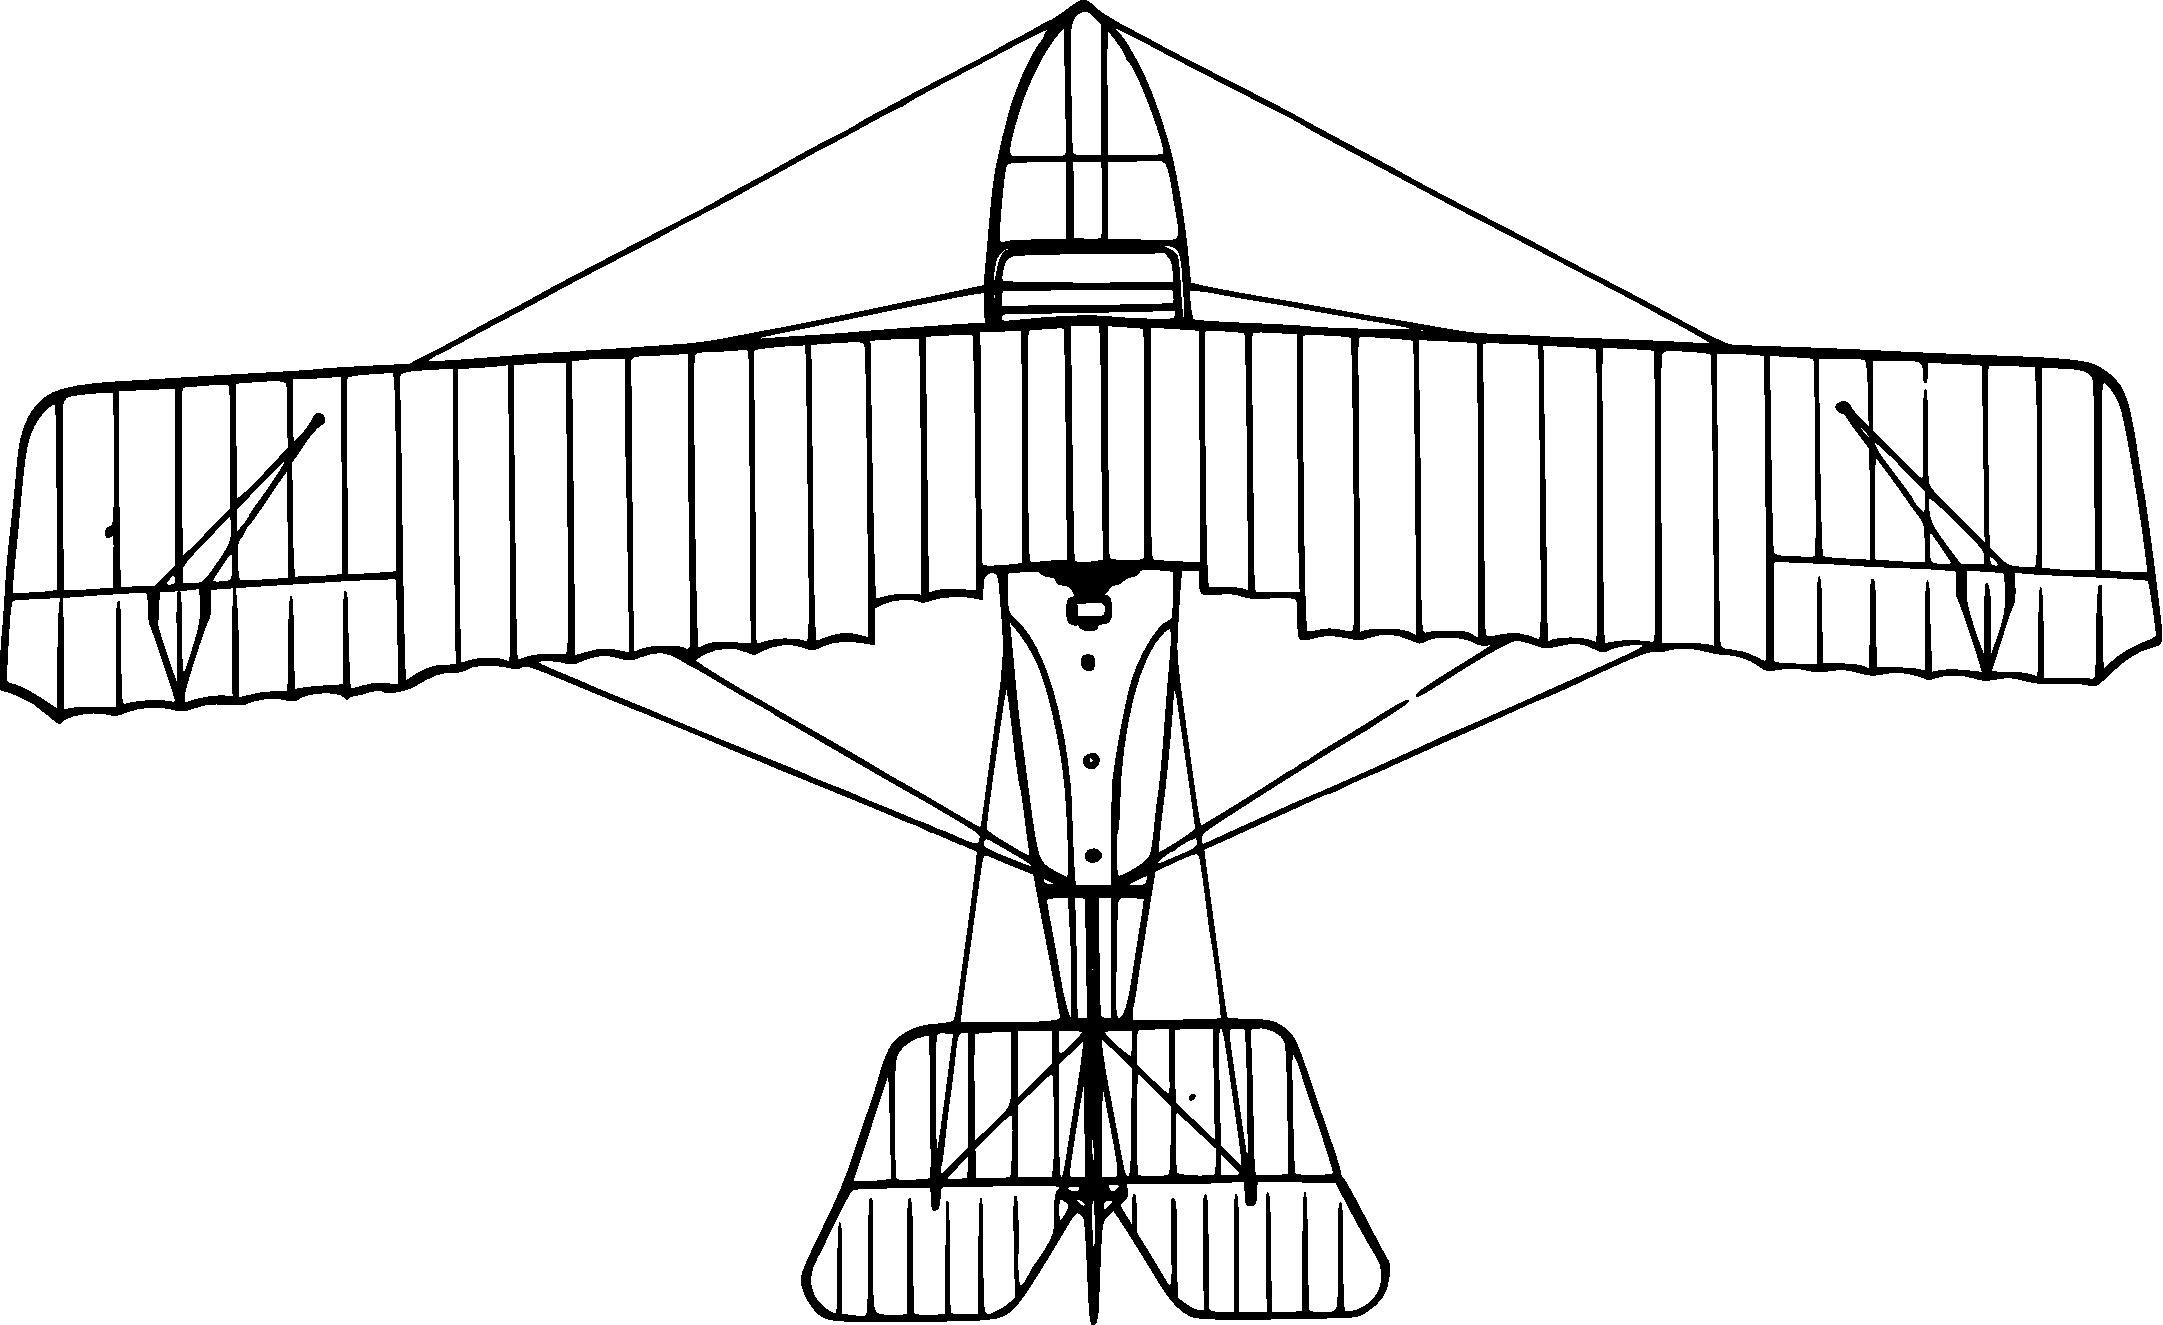
\includegraphics[width=.4\linewidth]{img/liftarn-Grigorovich-M-5-aircraft-top-view.pdf}
\end{flushright}
 
\begin{pbox}{ほそながいところ$\star\star$}{夏合宿2012}
  
馬車$n$台の出発時刻を調整して,条件を満たしながら全ての馬車がゴール地
点に到着するまでにかかる時間の最小値を求める.

\aojid{2427}
\end{pbox}

\begin{pbox}{Guesswork$\star\star$}{11th Polish Olympiad in Informatics}
  9個の数が順に与えられるので,一つづつ与えられた時点でそれが全体の何番目かを答える.9個すべてに回答した時点ですべて正解だったら勝ち.勝率を(100点がとれるくらいまで)最大化する戦略を実現せよ.

\url{http://main.edu.pl/en/archive/oi/11/zga}

(この問題は現在judgeが動いていない)
\end{pbox}


難易度が高い問題は,一学期履修した後に取り組むことが適切な場合もある.
 
\chapter{整数と連立方程式}

\begin{versionbeta}

\section{素因数分解、素数、ユークリッドの互除法など}

\begin{psbox}{Prime Factorize}{AOJ}
整数を素因数分解する

\aojid{NTL_1_A}
\end{psbox}
小さい数から順に割り切れるか試すと良い.被除数の平方根より大きな数で割
る必要はない(なぜか?)

\begin{psbox}{Greatest Common Divisor}{AOJ}
最大公約数を求める。  

\aojid{ALDS1_1_B}
\end{psbox}

\textbf{ユークリッドの互除法}というアルゴリズムが定番である.上記の問題の解説や\pcaojbook[pp.~441--443],\pccbook[pp.~107--]参照.
最大公約数を利用して簡単に最小公倍数も求められる(\aojid{NTL_1_C}  ).


\begin{psbox}{Sum of Prime Numbers}{PC甲子園2004}
与えられた数$n$に対して,素数を小さい方から並べた時に$n$番目の素数までの和を出力せよ。

\aojid{0053}  
\end{psbox}

\textbf{エラトステネスの篩}というアルゴリズムが定番である.
はじめに,数が素数かどうかを記録する大きな配列を用意し,すべての数が素数であるとしておく.2の倍数を2を除いて消去する,3以外の3の倍数を消去する,5以外の5の倍数を消去する.というように「まだ消されていない中で最大の数を素数として残した後、その倍数を消去する」という手順を繰り返す.判定したい最大の素数の平方根より大きな素数については,その倍数を消す必要はない.\pcaojbook[pp.~438--439]参照.


\begin{pbox}{Galaxy Wide Web Service}{夏合宿2009}
Webサービスに,様々な惑星から周期的なアクセスがある.
惑星$i$の,一日の時間は$1\le d_i \le 24$時間で,今の時刻は$t_i$時である.各惑星からのアクセス量はその惑星の時刻のみに依存して決まる.(幸いなことにどの惑星の時刻も地球の1時間が単位である.)
最もアクセスが多くなる時間帯のアクセス量を求めよ.

\aojid{2162}
\end{pbox}

方針:
\begin{itemize}
\setlength{\itemsep}{0pt}
\item もし全周期求められればだいたい分かる\\
サンプル入力のように(1 2 3 4)と(2 1)という惑星であれば、\\
\begin{tabular}{l|rrrrrrrr}
地球時間& 0 & 1 & 2 & 3 & 4 & 5 & 6 &7\\\hline
  惑星1 & 1 & 2 & 3 & 4 & 1 & 2 & 3 & 4\\
  惑星2 & 2 & 1 & 2 & 1 & 2 & 1 & 2 & 1\\\hline
  合計  & 3 & 3 & 5 & 5 & 3 & 3 & 5 & 5
\end{tabular}\\
と,アクセス数は4時間の周期の繰り返しとなるので答えは5
\item 全周期は? 惑星の時間数の最小公倍数.1から24まで全ての時間が揃うと,5354228880になる(無理)
\item 13, 17, 19, 23を特別扱いする.残りの数の最小公倍数は55440となる.この時刻であれば列挙可能である.
特別扱いした4つの数は,他のどの周期とも互いに素なので互いの最大値が重なる時刻がやがてあらわれる.つまり別に最大を求めて,全ての和を取ると良い.
\end{itemize}

入力と整形: 1-24時間周期の惑星毎にアクセス数をまとめる(t時間のずれも吸収する)\\
\begin{cbox}
    while (cin >> N && N) {
        int Q[25][25] = {{0}}; // Q[d][i] d周期のi時間目の量 (0<=i<d) 
        for (int i=0; i<N; ++i) {
            cin >> d >> t;
            for (int j=0; j<d; ++j) { 
                cin >> q;
                Q[d][(j+d-t)
            }
        }
        //この辺で答えを計算する
    }
\end{cbox}

\begin{rbox}
while true
  $N = gets.to_i
  break if $N == 0
  $Q = {}
  (1..$N).each {
    d, t, *q = gets.split(" ").map{|s| s.to_i}
    q.rotate!(t)
    unless $Q[d]
      $Q[d] = q
    else
      (0..d-1).each {|i| $Q[d][i] += q[i] }
    end
  }
  # この辺で答えを求める
end
\end{rbox}

ここまでの処理で,$1\le d \le 24$に対してQ[d][0]からQ[d][d-1]にその周期のアクセス数が格納されているので,適宜組み合わせる.

\begin{cbox}
const int L = 16*9*5*7*11;
        int sum = 0, T[L] = {0};
        for (int d=1; d<=24; ++d) {
            if (d == 13 || d == 17 || d == 19 || d == 23 || d == 1)
                sum += /*(Q[d][0]からQ[d][d-1]の最大値)*/;
            else
                for (int i=0; i<L; ++i) T[i] += Q[d][i
        }
        cout << sum + /*(T[0]からT[L-1]の最大値)*/ << endl;
\end{cbox}

\begin{rbox}
L = 16*9*5*7*11
  # 答えを計算するあたり
  sum = 0
  $T = Array.new(L,0)
  $Q.each{|d,q|
    if d == 13 || d == 17 || d == 19 || d == 23 || d == 1
      sum += q.max
    else
      (0..L-1).each { |i| $T[i] += q[i
    end
  }
  # sumと\$T.maxが答え
\end{rbox}

この問題では1から24までという制約があったために最小公倍数をあらかじめ
手で計算したが,計算機を用いて計算する場合は\jindex{ユークリッドの互助
  法}{ゆーくりっどのごじょほう}(\pccbook[pp.~107--])を用いると良い.

\begin{cbox}
int gcd(int a, int b) {
  if (a < b) swap(a,b);
  return b == 0 ? a : gcd(b, a
}  
\end{cbox}

\begin{pbox}{Extended Euclid Algorithm}{AOJ}
与えられた2つの整数 $a$, $b$ について $ax+by=\mbox{gcd}(a,b)$ の\cemph{整数}解 $(x,y)$を求めよ.

\aojid{NTL_1_E}
\end{pbox}
\jindex{拡張ユークリッド互除法}{かくちょうゆーくりっどのごじょほう}で求められる.
ユークリッド互除法が行っている計算で付随して求められる情報を活用する.

\begin{tipsbox}{逆元}
数え上げなどで「答えを$M=10^9+7$で割った余りを求めよ」という指示を持つ問題がある.
そのような場合に,$(p+q)\%M = ((p\%M)+(q\%M))\%M$, $(p\cdot q)\%M = ((p\%
M)\cdot(q\% M))\%M$などの関係を利用して,途中段階から剰余を取ると良い.多倍
長整数などを用いることなく,効率的に計算できるためである.ここで除算に
ついては,$(p/q)\%M = (p\cdot q^{-1})\%M$と変換する必要がある.$q^{-1}$とは,$(q\cdot q^{-1})\%M$を満たすような整数,$q$の\jindex{逆元}{ぎゃくげん}である.整数$q$と$M$が互いに素である時はつまり$\text{gcd}(q,M)=1$であるので,$(q,M)$についての拡張ユークリッド互除法により,$q^{-1}$を得ることが出来る.
\end{tipsbox}

\begin{pbox}{中国剰余定理}{古典}
  「$3$で割ると$2$余り、$5$で割ると$3$余り、$7$で割ると$2$余る数は何か」
一般に互いに素な整数$a,b,c$に対する剰余$a',b',c'$に対して,
  「$a$で割ると$a'$余り、$b$で割ると$b'$余り、$c$で割ると$c'$余る数」を一つ求める関数を作成せよ.

オンラインジャッジに適切な問題がなさそうなので,この問題は各自で入出力を作ってテストすること.テストしたデータをソースコードに添えること.
\end{pbox}

巨大な数を伴う計算を行う場合に,すべてを多倍長整数で計算すると計算コストが大きい.代わりに,複数の素数に対する剰余を計算して,最後に復元すると計算の効率が良い.
囲碁(19路盤)の合法局面の数\footnote{208168199381979984699478633344862770286522453884530548425639456820927419612738015378525648451698519643907
259916015628128546089888314427129715319317557736620397247064840935 (\url{DOI: 10.1007/978-3-319-50935-8_17})}は,このように求められた.


\section{連立方程式を解く}

\subsection{言語機能: valarray}

数値ベクトル (行列の行,あるいは列など)を扱う場合は \texttt{valarray}が便利である.

\begin{cbox}
#include <valarray>
valarray<int> V(0, N);  // 要素数Nの整数のベクトルを作成,各要素は0
V = 3; // 全要素を3に
V[0] = 1;
V *= 10; // 全要素を10倍に
V 

// 最大値 最小値 合計
cout << V.max() << ' ' << V.min() << ' ' << V.sum() << endl;

valarray<int> U(2, N);
V += U; // 各要素の和

// slice(initial, length, step)
V[slice(1,3,2)] = -3; // V[1] = V[3] = V[5] = -3
\end{cbox}

\subsection{連立方程式}

\begin{pbox}{Awkward Lights}{アジア地区予選2010}

ライトがグリッド状に並んでいる.
あるライトのスイッチを押すとそのライトに加えてマンハッタン距離$d$にあるライトのon/offの状態が変わる.全部のライトを消すことが出来るか?

\aojid{1308}

\end{pbox}

考え方: 2回以上スイッチを押しても意味がないので,各スイッチは押すか押
さないかのどちらか.各スイッチに$0$から$MN-1$の番号を振り,押したかど
うかを$x_i \in \{0,1\}$であらわす.
行列$A$は$MN$行/列で,要素$a_{ij}$は,スイッチ$i$を押すとライト$j$に影響があることを示すとする.
行列$A$とベクトル$x$の積は,変化を受けたスイッチを表すベクトルとなる.
各ランプが最初についていたかどうかを$b_i$で表すとして,$Ax = b$に解があるかどうかを求める(ただしすべての演算をmod $2$で行う).

掃き出していって行列左下の三角部分を0にした時に、どのスイッチでも消せな
いライトが残らなければ成功

入力
\begin{cbox}
typedef valarray<int> array_t;
int M, N, D;
int main() {
    while (cin >> M >> N >> D && M) {
        valarray<array_t> A(array_t(0, M*N+1), M*N);
        for (int i=0; i<M*N; ++i) {
            cin >> A[i][M*N];
            for (int j=0; j<M*N; ++j) {
                int x0=i
                int d=abs(x0-x1)+abs(y0-y1);
                if (d==0 || d==D) A[i][j] = 1;
            }
        }
        cout << solve(A) << endl;
    }
} 
\end{cbox}

Aは$MN$行,$MN+1$列の行列で,右端の列は最初についているかどうか,他の列の
要素はi個目のスイッチを押したときにj個目のライトが切り替わるかを表す.
$A[i]$ はi行目を表し,各行は\texttt{valarray<int>}一つに対応する.
(慣れたら行列全体をひとつの\texttt{valarray<int>}で表したほうが効率が良い)

計算
\begin{cbox}
int solve(valarray<array_t>& A) {
    int p = 0;                  // top $\rightarrow$ bottom
    for (int i=0; i<M*N; ++i) { // left $\rightarrow$ right
        int r = // 「p以降で A[r][i]!=0 の行」
        if (/*適切なrが存在しなければ*/) continue;
        swap(A[p], A[r]);
        for (int j=p+1; j<M*N; ++j)
            if (A[j][i]) {
                // 行A[j]に行A[p]を足しこむ,A[j]\%=2を忘れずに
            }
        ++p;
    }
    for (int r=0; r<M*N; ++r)
        if (/* A[r][M*N] が非0で,A[r]の要素がそれ以外0だと*/) return 0;
    return 1;
}
\end{cbox}


\begin{pbox}{Strange Couple$\star$}{夏合宿2009}

道路と交差点の一覧が与えられる.標識がない交差点ではUターンも含めて等確率でランダムに道を選び,標識がある交差点ではそこから目的地までの最短で到達できるルートを(複数あればランダムに選ぶ)人がいる.出発地から目的地までに通る距離の合計の期待値を求めよ.

\aojid{2171}
\end{pbox}

最短路と連立方程式:
まず,ダイクストラ法などで目的地から各交差点までの距離を求める.続いて,各交差点から出発した場合の期待値を変数として,隣合う交差点から出発した場合の期待値との関係から連立方程式を立てる.

最短路の求め方は後日扱うので,まだ学んでいない場合は後で取り組むと良い.

\section{その他の練習問題}

\begin{pbox}{Afternoon Tea$\star$}{Polish Olympiad in Informatics 2011}
紅茶とミルク、どちらをより多く飲んだか?

\url{http://main.edu.pl/en/archive/amppz/2011/her}
\end{pbox}

\begin{pbox}{Making Change}{codechef}
ある国の硬貨の価値は D[1], ..., D[N] である.金額 C (とても大きい) を
この国の硬貨で支払う方法は何通り?
ただし D[1], ..., D[N] は相異なりどの 2 つも互いに素.  

\url{http://www.codechef.com/problems/CHANGE}
\end{pbox}

\chapter{補間多項式と数値積分}\label{chapter:integral}

\section{Lagrange補間多項式}

3点 $(a,v_a), (b,v_b), (c, v_c)$を通る2次の多項式は次のように一意に定まる:
\begin{equation}
L(x) = \frac{(x-b)(x-c)}{(a-b)(a-c)}v_a + \frac{(x-a)(x-c)}{(b-a)(b-c)}v_b + \frac{(x-a)(x-b)}{(c-a)(c-b)}v_c. \label{eq:interpolate3}  
\end{equation}
一般に,与えられた$N$個の点を通る次数最低の多項式は一意に定まる:
$$
L(x) = \sum_{k=0}^{N-1} \left(\prod_{i\neq k}\frac{(x-x_i)}{(x_k-x_i)}\right)\cdot{}v_{x_k}.
$$

(この式でくらっとした場合は,以下を無視して\ref{section:numerical-integration}節へ進んで良い.)

\begin{pbox}{Find the Outlier}{アジア地区予選2012}
秘密の多項式$f(x)$の次数$d$と$d+3$個の点,$(0,v_0), (1,v_1), \cdots,(d+2,v_{d+2})$が与えられる.
点$(i,v_i)$は$f(i)=v_i$を満たすが,例外として
一点$(i',v_{i'})$のみ$v_{i'}$に$1.0$以上の誤りを含む.その点$i'$を求めよ.入力は$10^{-6}$より大きな誤差を含まない.

\aojid{1328}
\end{pbox}

方針:
\begin{itemize}
\setlength{\itemsep}{0pt}
\item $d+1$個の点を選んでLagrange補間多項式を作る.その式の値と,選ばれなかった点が一致するかを考える.
\item $i'$を除いた$d+2$個の点についてだけ考えると,どの$d+1$個の点で作られた補間多項式も$f$と一致し,残りの1点を通る.
\item 点$i'$を含む$d+2$個の点については,同様の補間多項式が残りの1つの点と一致しないような($d+1$個と$1$個)の点の選び方がある.
\end{itemize}

\begin{center}
\begin{tikzpicture}[gnuplot]
\path (0.000,0.000) rectangle (12.500,8.750);
\gpcolor{color=gp lt color border}
\gpsetlinetype{gp lt border}
\gpsetlinewidth{1.00}
\draw[gp path] (1.012,1.168)--(1.192,1.168);
\draw[gp path] (10.697,1.168)--(10.517,1.168);
\node[gp node right] at (0.828,1.168) {-10};
\draw[gp path] (1.012,2.171)--(1.192,2.171);
\draw[gp path] (10.697,2.171)--(10.517,2.171);
\node[gp node right] at (0.828,2.171) { 0};
\draw[gp path] (1.012,3.175)--(1.192,3.175);
\draw[gp path] (10.697,3.175)--(10.517,3.175);
\node[gp node right] at (0.828,3.175) { 10};
\draw[gp path] (1.012,4.179)--(1.192,4.179);
\draw[gp path] (10.697,4.179)--(10.517,4.179);
\node[gp node right] at (0.828,4.179) { 20};
\draw[gp path] (1.981,0.616)--(1.981,0.796);
\draw[gp path] (1.981,4.881)--(1.981,4.701);
\node[gp node center] at (1.981,0.308) { 0};
\draw[gp path] (3.918,0.616)--(3.918,0.796);
\draw[gp path] (3.918,4.881)--(3.918,4.701);
\node[gp node center] at (3.918,0.308) { 1};
\draw[gp path] (5.855,0.616)--(5.855,0.796);
\draw[gp path] (5.855,4.881)--(5.855,4.701);
\node[gp node center] at (5.855,0.308) { 2};
\draw[gp path] (7.792,0.616)--(7.792,0.796);
\draw[gp path] (7.792,4.881)--(7.792,4.701);
\node[gp node center] at (7.792,0.308) { 3};
\draw[gp path] (9.729,0.616)--(9.729,0.796);
\draw[gp path] (9.729,4.881)--(9.729,4.701);
\node[gp node center] at (9.729,0.308) { 4};
\draw[gp path] (1.012,4.881)--(1.012,0.616)--(10.697,0.616)--(10.697,4.881)--cycle;
\node[gp node right] at (8.869,2.484) {all points};
\gpcolor{rgb color={0.780,0.141,0.227}}
\gpsetpointsize{12.00}
\gppoint{gp mark 1}{(1.981,2.272)}
\gppoint{gp mark 1}{(3.918,2.573)}
\gppoint{gp mark 1}{(5.855,3.376)}
\gppoint{gp mark 1}{(7.792,3.777)}
\gppoint{gp mark 1}{(9.729,4.680)}
\gppoint{gp mark 1}{(9.691,2.484)}
\gpcolor{color=gp lt color border}
\node[gp node right] at (8.869,1.809) {interpolation (x=0,1,4)};
\gpcolor{rgb color={0.000,0.573,0.314}}
\gpsetlinetype{gp lt plot 1}
\gpsetlinewidth{2.00}
\draw[gp path] (9.053,1.809)--(10.329,1.809);
\draw[gp path] (1.012,2.197)--(1.110,2.202)--(1.208,2.208)--(1.305,2.214)--(1.403,2.221)
  --(1.501,2.228)--(1.599,2.236)--(1.697,2.245)--(1.795,2.253)--(1.892,2.263)--(1.990,2.273)
  --(2.088,2.283)--(2.186,2.294)--(2.284,2.306)--(2.382,2.318)--(2.479,2.330)--(2.577,2.343)
  --(2.675,2.357)--(2.773,2.371)--(2.871,2.385)--(2.969,2.400)--(3.066,2.416)--(3.164,2.432)
  --(3.262,2.449)--(3.360,2.466)--(3.458,2.483)--(3.556,2.501)--(3.653,2.520)--(3.751,2.539)
  --(3.849,2.559)--(3.947,2.579)--(4.045,2.600)--(4.143,2.621)--(4.240,2.643)--(4.338,2.665)
  --(4.436,2.688)--(4.534,2.711)--(4.632,2.735)--(4.729,2.759)--(4.827,2.784)--(4.925,2.809)
  --(5.023,2.835)--(5.121,2.861)--(5.219,2.888)--(5.316,2.915)--(5.414,2.943)--(5.512,2.971)
  --(5.610,3.000)--(5.708,3.030)--(5.806,3.060)--(5.903,3.090)--(6.001,3.121)--(6.099,3.152)
  --(6.197,3.184)--(6.295,3.217)--(6.393,3.250)--(6.490,3.283)--(6.588,3.317)--(6.686,3.352)
  --(6.784,3.387)--(6.882,3.422)--(6.980,3.458)--(7.077,3.495)--(7.175,3.532)--(7.273,3.569)
  --(7.371,3.608)--(7.469,3.646)--(7.566,3.685)--(7.664,3.725)--(7.762,3.765)--(7.860,3.806)
  --(7.958,3.847)--(8.056,3.888)--(8.153,3.931)--(8.251,3.973)--(8.349,4.017)--(8.447,4.060)
  --(8.545,4.105)--(8.643,4.149)--(8.740,4.195)--(8.838,4.240)--(8.936,4.287)--(9.034,4.333)
  --(9.132,4.381)--(9.230,4.428)--(9.327,4.477)--(9.425,4.526)--(9.523,4.575)--(9.621,4.625)
  --(9.719,4.675)--(9.817,4.726)--(9.914,4.778)--(10.012,4.829)--(10.108,4.881);
\gpcolor{color=gp lt color border}
\node[gp node right] at (8.869,1.134) {interpolation (x=1,2,3)};
\gpcolor{rgb color={0.365,0.388,0.620}}
\gpsetlinetype{gp lt plot 2}
\draw[gp path] (9.053,1.134)--(10.329,1.134);
\draw[gp path] (1.012,0.616)--(1.110,0.697)--(1.208,0.776)--(1.305,0.855)--(1.403,0.932)
  --(1.501,1.009)--(1.599,1.084)--(1.697,1.159)--(1.795,1.232)--(1.892,1.304)--(1.990,1.376)
  --(2.088,1.446)--(2.186,1.515)--(2.284,1.584)--(2.382,1.651)--(2.479,1.717)--(2.577,1.782)
  --(2.675,1.847)--(2.773,1.910)--(2.871,1.972)--(2.969,2.033)--(3.066,2.093)--(3.164,2.152)
  --(3.262,2.210)--(3.360,2.267)--(3.458,2.323)--(3.556,2.378)--(3.653,2.432)--(3.751,2.485)
  --(3.849,2.537)--(3.947,2.588)--(4.045,2.638)--(4.143,2.687)--(4.240,2.735)--(4.338,2.781)
  --(4.436,2.827)--(4.534,2.872)--(4.632,2.916)--(4.729,2.958)--(4.827,3.000)--(4.925,3.041)
  --(5.023,3.080)--(5.121,3.119)--(5.219,3.156)--(5.316,3.193)--(5.414,3.228)--(5.512,3.263)
  --(5.610,3.296)--(5.708,3.329)--(5.806,3.360)--(5.903,3.391)--(6.001,3.420)--(6.099,3.449)
  --(6.197,3.476)--(6.295,3.502)--(6.393,3.527)--(6.490,3.552)--(6.588,3.575)--(6.686,3.597)
  --(6.784,3.618)--(6.882,3.639)--(6.980,3.658)--(7.077,3.676)--(7.175,3.693)--(7.273,3.709)
  --(7.371,3.724)--(7.469,3.738)--(7.566,3.751)--(7.664,3.763)--(7.762,3.774)--(7.860,3.784)
  --(7.958,3.793)--(8.056,3.801)--(8.153,3.808)--(8.251,3.813)--(8.349,3.818)--(8.447,3.822)
  --(8.545,3.825)--(8.643,3.827)--(8.740,3.827)--(8.838,3.827)--(8.936,3.826)--(9.034,3.823)
  --(9.132,3.820)--(9.230,3.815)--(9.327,3.810)--(9.425,3.804)--(9.523,3.796)--(9.621,3.788)
  --(9.719,3.778)--(9.817,3.768)--(9.914,3.756)--(10.012,3.743)--(10.110,3.730)--(10.208,3.715)
  --(10.306,3.699)--(10.404,3.683)--(10.501,3.665)--(10.599,3.646)--(10.697,3.627);
\gpcolor{color=gp lt color border}
\gpsetlinetype{gp lt border}
\gpsetlinewidth{1.00}
\draw[gp path] (1.012,4.881)--(1.012,0.616)--(10.697,0.616)--(10.697,4.881)--cycle;
\gpdefrectangularnode{gp plot 1}{\pgfpoint{1.012cm}{0.616cm}}{\pgfpoint{10.697cm}{4.881cm}}
\end{tikzpicture}
\begin{flushleft}
1つ目のサンプル入力の例: outlierである(2,12)を外した3点で補間するとどの場合も同じ関数が得られ,outlierの1点は外れるが,補間に使用しなかった残りの一点を通る(緑破線).outlierである(2,12)を含む3点で補間すると,残りの2点を外れる(青点線).
\end{flushleft}
\end{center}

点$f(n)$を,点$(n,v_n)$と$(E,v_E)$を除いた$d+1$個の点から求める関数\texttt{interpolate(n,E)}は以下のように作ることができる.

\begin{cbox}[emph={interpolate}]
int D;
double V[16];
double interpolate(int n, int E) {
    // L(n)を補間多項式により計算する
    // ただし点(n,V[n])と(E,V[E])は使わない
    double sum = 0.0;
    for (int k=0; k<D+3; ++k) {
        if (/*kがnかEなら*/) continue;
        double p = V[k];
        for (int i=0; i<D+3; ++i)
            if (! (/*iがkでもnでもEでもなければ*/))
                p *= (...-i)/(double)(k-i);
        sum += p;
    }
    return sum;
}
\end{cbox}

\begin{pybox}[emph={interpolate}]
# 配列Vに値が入っているとする
def interpolate(n, e):
  total = 0.0
  for k in range(len(V)):
    if ... # kがnかEなら
        continue 
    p = V[k]
    for i in range(len(V)):
        if  ... # iがkでもnでもEでもなければ
            p *= 1.0*(n-i)/(k-i)
    total += p
  return total
\end{pybox}

この関数\texttt{interpolate}を用いると,点$(E,V_E)$が異常だったと仮定して,残りの$d+2$個の点に異常がないか調べる関数\texttt{outlier(E)}を次のように簡単に作ることが出来る.

\begin{cbox}[emph={outlier},emph={[2]interpolate}]
bool outlier(int E) {
    for (int i=0; i<D+3; ++i) {
        if (i==E) continue;
        double p = interpolate(i, E);
        if (/*pとV[i]の絶対値(abs)が0.1より離れていたら*/)
            return false;
    }
    return true;
}
\end{cbox}

\begin{pybox}[emph={outlier},emph={[2]interpolate}]
def outlier(e):
    for i in range(len(V)):
        if i == e:
            continue 
        p = interpolate(i, e)
        if ... # pとV[i]の絶対値(abs)が0.1より離れていたら
            return False 
    return True  
\end{pybox}

\begin{cbox}[emph={},emph={[2]outlier,interpolate}]
#include<iotream>
#include<cmath>
// この辺に上記の関数を定義する
int main() {
    while (cin >> D && D) {
        for (int i=0; i<D+3; ++i) cin >> V[i];
        for (int i=0; i<D+3; ++i)
            if (outlier(i)) { // iを無視すれば全て整合する
                cout << i << endl;
                break;
            }
    }
}
\end{cbox}

\begin{pybox}[emph={},emph={[2]outlier,interpolate}]
# global変数Vと上記の関数を事前に定義しておく  
while True:
  d = int(input())
  if d == 0:
      break 
  V = [float(input()) for _ in range(d+3)]
  for i in range(d+3):
      if outlier(i): # iを無視すれば全て整合する
          print(i)
          break  
\end{pybox}

\section{数値積分とシンプソン公式}\label{section:numerical-integration}

\begin{psbox}{Integral}{PC甲子園2003}
長方形の和を用いて面積の近似値を求めよ.

\aojid{0014}
\end{psbox}

関数$f(x)$の区間$[a,b]$の定積分$\displaystyle\int_a^b f(x) dx$を求めたい.解析的に解く方法以外に,数値計
算で近似値を求める種々の方法が存在する.もっとも簡便な方法は,区間を細
かく分けて長方形の面積の和で近似するものである.(例題の話題はここで区切り)

\subsection{台形公式}

小分けにした短冊部分について,
長方形を台形に変更すると,分割数に対応する精度を高めることができる.
分割幅を$h$とすると誤差は$O(h)$から$O(h^2)$に改善する(計算誤差の影響を無視すれば,刻みを10倍細かく取ると,精度が100倍改善すると予想できる).

\begin{center}
\begin{tikzpicture}[y=5mm]
\coordinate (p1) at (0.7,3.25);
\coordinate (p2) at (1,3.3);
\coordinate (p3) at (2,2.5);
\coordinate (p4) at (3,2.5);
\coordinate (p5) at (4,3.5);
\coordinate (p6) at (5,4.1);
\coordinate (p7) at (6,3.4);
\coordinate (p8) at (6.3,4.1);

\fill[gray!10] 
  (p2|-0,0) -- (p2) -- (p3) -- (p4) -- (p5) -- (p6) -- (p7) -- (p7|-0,0) -- cycle;
\fill[gray!30] (p4|-0,0) -- (p4) -- (p5) -- (p5|-0,0) -- cycle;
\draw[thick,dotted,iblue] (p1) to[out=70,in=180] (p2);
\draw[thick,dotted,iblue] (p7) to[out=0,in=230] (p8);
\draw[thick,iblue]
  (p2) to[out=0,in=150] 
  (p3) to[out=-50,in=205] (p4) to[out=27,in=210] 
  (p5) to[out=33,in=150] (p6) to[out=-30,in=180] (p7);
\draw[] (p2) -- (p3) -- (p4) -- (p5) -- (p6) -- (p7);
\foreach \n/\texto in
         {2/{a=x_0},3/{},4/{x_i},5/{x_{i+1}},6/{},7/{b=x_n}}
{
  \draw[dashed] (p\n|-0,0) -- (p\n);
  \node[below,text height=1.5ex,text depth=1ex,font=\small] at
  (p\n|-0,0) {$\texto$};
}
\draw[->] (-0.5,0) -- (7,0) coordinate (x axis);
\draw[->] (0,-0.5) -- (0,6) coordinate (y axis);
\node[below] at (x axis) {$x$};
\node[left] at (y axis) {$y$};
\node[above,text=iblue] at (p6) {$y=f(x)$};
\end{tikzpicture}
\end{center}

\begin{tipsbox}{応用}
  実際には数値誤差の影響で$h$を小さくしてもある程度で,誤差は減少しな
  くなる.
  各項の丸め誤差が$\epsilon=10^{-16}$と予想される時,適切な$h$はどのように見積もれば良いか?
\end{tipsbox}

\subsection{シンプソン公式}

シンプソン公式
(Simpson's rule)では,直線の代わりに二次式で近似し,精度は$O(h^4)$に改善する.
先ほどまでと記法が異なるが$a=x_i,\ b=x_{i+1}$として,
区間内の三点$(a,f(a))$, $(\frac{a+b}{2},f(\frac{a+b}{2}))$, $(b,f(b))$を使った補間多項式(式(\ref{eq:interpolate3}))で表現して整理すると,その区間の面積は以下のように近似できる:
$$
\int_a^b f(x) dx \,\approx\, \frac{b-a}{6}\left(f(a)+4f\left(\frac{a+b}{2}\right)+f(b)\right).
$$

もし区間内で$f(x)$が二次以下の多項式であれば,計算誤差を無視すれば正確な値を得ることが出来る.

\begin{pbox}{One}{立命館合宿2013}
  窓枠内に見えている山々と空との境界の長さを求めよ.入力の制約から山の頂点は窓枠内(境界含む)に存在する.

\url{http://judge.u-aizu.ac.jp/onlinejudge/cdescription.jsp?cid=RitsCamp13Day2&pid=I}
\end{pbox}
注: 区間$x\in[a,b]$の$f(x)$の周長は,$f(x)$の導関数を$f'(x)$として$\int_a^b \sqrt{1+f'(x)^2}dx$で与えられる.

山と空の境界をどの放物線が与えるかは,場所によって異なる.そこで$x$軸で
区間に分けて,各区間事の周長を合計すると良い.分割方法は,各放物線同士
の交点(あれば)や窓の下端との交点(あれば)の$x$座標を列挙し,それらを用い
て窓内のを分割すれば十分かつ,区間の数も問題ない範囲である.各区間では
まったく山が見えないもしくは,一つの放物線が空との境界をなす.どの放物
線が一番上にあるかは,区間の中央の$x$での高さで比較すれば求まる.積分は,
数値計算がお勧め.

\begin{pbox}{Intersection of Two Prisms$\star$}{アジア地区予選2010}

z軸方向に無限の高さを持つ多角柱P1と,y軸方向に無限の高さを持つ多角柱P2の共通部分の体積を求めよ.

\aojid{1313}
\end{pbox}

方針(\pccbook[pp.~236--]): 求める立体を平面$x=a$で切断した断面を考える.
断面は面積を持たないか,またはy軸とz軸に平行な長方形になるから,その面積を$x$軸方向に積
分して体積を求める.区間は立体の頂点の存在するx座標で区切る.

あるx座標での切断面でのy軸またはx軸の幅を求める関数
\texttt{width(polygon, x)}は,たとえば以下のように与えられた多角
形の辺を一巡して求めることができる.

\begin{pybox}[emph={width},emph={[2]w}]
def width(polygon, x): # polygon にx-yまたはx-z平面の座標が順に入っている
    w = []
    for i in range(len(polygon)):
        p, q = polygon[i], polygon[(i+1)
        if p[0] == x:
            w.append(p[1])
        elif (p[0] < x and x < q[0]) or (p[0] > x and x > q[0]):
            x0, y0 = p[0], p[1]
            x1, y1 = q[0], q[1]
            w.append(y0 + 1.0*(y1-y0)*(x-x0)/(x1-x0))
    assert len(w) > 0
    return max(w) - min(w)
\end{pybox}

この関数を利用して,体積を求める関数\texttt{volume}を,たとえば以下の
ように作成できる.なお\texttt{\$P1}は多角形P1の(x,y)座標を順に格納した
配列,\texttt{\$P2}を多角形P2の(x,z)座標を順に格納した配列,  \texttt{\$X}をP1とP2に登場するX座標を昇順に格納した配列とする.

\begin{pybox}[emph={volume},emph={[2]width,total}]
def volume(Pxy,Pxz,X):
    X = sorted(set(X))
    total = 0.0
    xmin = max(min(Pxy)[0], min(Pxz)[0])
    xmax = min(max(Pxy)[0], max(Pxz)[0])
    for i in range(len(X)-1):
        a, b = X[i], X[i+1]
        if not (xmin <= a and a <= xmax and xmin <= b and b <= xmax):
            continue
        m = (a+b)/2.0
        va = width(Pxy, a)*width(Pxz, a)
        vb = width(Pxy, b)*width(Pxz, b)
        vm = width(Pxy, m)*width(Pxz, m)
        area = ... # (a,va), (m,vm), (b,vb)を通る区間[a,b]の定積分
        total += area
    return total
\end{pybox}
\section{道具としての Fast Fourier Transform (FFT)}
(この節の説明はまだ書かれていない)

\begin{pbox}{Best Position$\star$}{Kuala Lumpur 2014}
  
農耕と牧畜の生産が最大になる場所を探す.畑候補は長方形領域で,それ以内
の畑パターンを重ねあわせた時に一致したマスで生産が生じる.

  \url{https://icpcarchive.ecs.baylor.edu/index.php?option=com_onlinejudge&Itemid=8&category=645&page=show_problem&problem=4820}
\end{pbox}

畑候補と畑パターンをそれぞれ多項式として表現して,その積の多項式のある係数が,ある場所で重ねあわせた時の領域の和になるように工夫する.

\begin{pbox}{Point Distance$\star$}{春コンテスト2013}
各セル(x,y)に,分子がいくつ入っているか$C_{xy}$で表される.すべての分
子のペアを考えた時の平均距離と距離毎のヒストグラムを示せ.

\aojid{2560}
\end{pbox}

二次元のFFTの練習.ヒストグラムは\texttt{long long}が必要.

\begin{pbox}{The Teacher's Side of Math$\star$}{アジア地区予選2007}
解の一つが$a^{1/m}+b^{1/n}$であるような、整数係数多項式を求めるプログラ
ム
を作成せよ.
($a,b$は互いに異なる素数、$m,n$は2以上の整数)

\aojid{1284}
\end{pbox}

ヒント: 
一般に $1$ の原始 $m$ 乗根を $\xi$, $1$ の原始 $n$ 乗根を $\eta$ として
$$
\prod_{j=0}^{m-1}\prod_{k=0}^{n-1}
(x-a^{1/m}\xi^j-b^{1/n}\eta^k)
$$
という多項式を作ると
$$
=\prod_{j=0}^{m-1}\{(x-a^{1/m}\xi^j)^n-b\}
=\prod_{k=0}^{n-1}\{(x-b^{1/n}\eta^k)^m-a\}
$$
と変形できることを利用する.

数が小さいので,適当に展開しても良いし,FFTを用いても良い.

\end{versionbeta}
 \chapter{区間の和/最大値/最小値と更新}

\begin{versionbeta}

\begin{itembox}[l]{概要}
  ある程度大きなデータを与えられたうえで,質問ごとにデータの一部を調査
するタイプの問題を考える.事前に準備をしておく($\approx$適切なデータ構造を用いる)ことで質問に効率的に答えられるようになる.ここでは一列あるいはグリッド上に並んだデータについて考える.
\end{itembox}

\section{累積和}

初めに,列$a_i$の先頭からの和 $S_{i+1} = \sum_{k=0}^i a_k$ を活用する
問題を考える.$S_0=0$とする.

\begin{psbox}{Maximum Sum Sequece}{PC甲子園2003}
整数の並び $a_1, a_2, a_3, \ldots, a_n$ で、連続した1つ以上の項の和の最大値を求
めよ.

注: もし$a_i$が非負なら当然すべての和が最大なので,負の数を含む.負の数を含む区間が最大になることもある.

\aojid{0022}
\end{psbox}

(これはmaximum subarray problemという問題で,列の長さを$N$として$O(N)$
の解き方がある.しかし,ストーリーの都合で全区間を調べて$O(N^2)$で解くことにする)

区間[i,j)の和,すなわち$\sum_{k=i}^{j-1} a_k$を定義通りに計算すると,
$j-i-1$回の加算が必要である.これを$j-i$によらず1回の演算で済ませた
い.
それには,事前に $S_0=0$, $S_{i+1} = \sum_{k=0}^i a_k = S_i+a_i$となる
ような補助変数$S$を用意しておけば良い.これを用いると,区間[i,j)の和は
  $S_j-S_i$で求められる.たとえば,$a_8+a_9+a_{10}+a_{11} = S_{12} - S_8$である.

\begin{center}
\begin{tikzpicture}[y=5mm]

\node[above right] (a0) at (0,0) [draw,thick,minimum width=1cm,minimum height=0.5cm] {$a_0$};
\node[above right] (a1) at (1,0) [draw,thick,minimum width=1cm,minimum height=0.5cm] {$a_1$};
\node[above right] (a2) at (2,0) [draw,thick,minimum width=1cm,minimum height=0.5cm] {$a_2$};
\node[above right] (a3) at (3,0) [thick,minimum width=1cm,minimum height=0.5cm] {$\ldots$};
\node[above right] (a7) at (4,0) [draw,thick,minimum width=1cm,minimum height=0.5cm] {$a_7$};
\node[above right] (a8) at (5,0) [draw,thick,minimum width=1cm,minimum height=0.5cm] {$a_8$};
\node[above right] (a9) at (6,0) [draw,thick,minimum width=1cm,minimum height=0.5cm] {$a_9$};
\node[above right] (a10) at (7,0) [draw,thick,minimum width=1cm,minimum height=0.5cm] {$a_{10}$};
\node[above right] (a11) at (8,0) [draw,thick,minimum width=1cm,minimum height=0.5cm] {$a_{11}$};
\node[above right] (a12) at (9,0) [draw,thick,minimum width=1cm,minimum height=0.5cm] {$a_{12}$};
\node[above right] (a13) at (10,0) [draw,thick,minimum width=1cm,minimum height=0.5cm] {$a_{13}$};
\node[above right] (a14) at (11,0) [thick,minimum width=1cm,minimum height=0.5cm] {$\ldots$};
\draw (0,0) to [out=-10,in=190] (5,0);
\node[] () at (2.5,-1) {$S_8$};
\draw (0,1) to [out=7,in=173] (9,1);
\node[] () at (5.5,2) {$S_{12}$};
\end{tikzpicture}
\end{center}

これを用いて,すべての区間の和を調べると求める最大値を得られる.

\begin{pbox}{A Traveler}{JOI 2009}
左右に行ったり来たりする旅程が与えられるので歩いた合計(の剰余)を求めよ.

\aojid{0549}  
\end{pbox}

考え方: 旅程の要素に「左に30個目の宿場に移動する」という指示があったと
して,30回の加算をすることは避けたい.そこで事前に各宿場について左端か
らの距離を事前に計算しておく.すると旅程の要素数である$M$回の加算で合計
の距離を求められる.

\subsection*{二次元の累積和}

同様の考え方は二次元にも応用できる:
補助変数を$S_{i+1,j+1} = \sum_{k=0}^i \sum_{l=0}^j a_{k,l}$ と定義する.
縦[i,i'), 横[j,j')の長方形領域の和は
$S_{i',j'} - S_{i,j'} - S_{i',j} + S_{i,j}$となる.(大きな長方形から余分にを引いて,引きすぎたものを調整する)
つまり,長方形領域の面積によらない定数回の演算で求めることができる.

\begin{center}
\begin{tikzpicture}

\draw (0,0) rectangle (6,4);
\draw[dotted] (2,0) -- (2,4);
\draw[dotted] (0,2.5) -- (6,2.5);
\node[below right] () at (0,4) [draw] {\small $a_{0,0}$};
\node[below right] () at (0,2.5) [draw] {\small $a_{i,0}$};
\node[below right] () at (2,2.5) [draw] {\small $a_{i,j}$};
\node[below right] () at (6,2.5) [draw,dotted] {\small $a_{i,j'}$};
\node[below right] () at (2,0) [draw,dotted] {\small $a_{i',j}$};
\node[below right] () at (6,0) [draw,dotted] {\small $a_{i',j'}$};
\node[] () at (1,1.25) {$C$};
\node[] () at (1,3.25) {$A$};
\node[] () at (4,1.25) {$D$};
\node[] () at (4,3.25) {$B$};
\node[] () at (10,2) {\vbox{\hbox{$A=S_{i,j}$}\hbox{$A+B=S_{i,j'}$}\hbox{$A+C=S_{i',j}$}\hbox{$A+B+C+D=S_{i',j'}$}}};
\end{tikzpicture}
\end{center}

\begin{psbox}{Maximum Sum Sequence II}{PC甲子園2003}
和が最大になる長方形領域を知りたい.

\aojid{0098}  
\end{psbox}

(この問題も縦横どちらかのmaximum subarray problemに変換することで,$O(N^3)$
で解ける.しかし,ストーリーの都合で全長方形区間を調べて$O(N^4)$で解く意図で掲載する)

\begin{pbox}{Planetary Exploration}{JOI 2010}
指定の長方形区域の資源の数を知りたい.

\aojid{0560}
\end{pbox}

\begin{pbox}{Coffee Central$\star$}{World Finals 2011}
カフェを開くのに最適な場所を知りたい.

\url{https://icpcarchive.ecs.baylor.edu/index.php?option=com_onlinejudge&Itemid=8&category=45&page=show_problem&problem=3133}
\end{pbox}

菱形の領域は45度回転させると扱いやすくなる場合がある.

\section{Binary Indexed Tree (Fenwick Tree)}

今度は処理の途中でデータ$a_i$の一部が変化する状況を考える.
前節のように補助変数$S$を使うと,質問には$O(1)$で回答できて効率が良いが
更新には$O(N)$かかってしまう.質問回答に$O(\log N)$のコストを許容することで,$O(\log N)$の更新を実現する手法を紹介する.(\pccbook[pp. 160--])

\begin{pbox}{Range Query - Range Sum Query}{AOJ}
区間の合計値を管理せよ  

\aojid{DSL_2_B}
\end{pbox}

\begin{center}
\begin{tikzpicture}[y=5mm]
\node[above right] (S8) at (0,6) [draw,thick,minimum width=8cm,minimum height=0.5cm] {$S_{1,8}$};
\node[above right] (S4) at (0,4) [draw,thick,minimum width=4cm,minimum height=0.5cm,fill=gray!15!] {$S_{1,4}$};
\node[above right] (S2) at (0,2) [draw,thick,minimum width=2cm,minimum height=0.5cm] {$S_{1,2}$};
\node[above right] (S6) at (4,2) [draw,thick,minimum width=2cm,minimum height=0.5cm,fill=gray!15!] {$S_{5,6}$};
\node[above right] (S1) at (0,0) [draw,thick,minimum width=1cm,minimum height=0.5cm] {$S_{1,1}$};
\node[above right] (S3) at (2,0) [draw,thick,minimum width=1cm,minimum height=0.5cm] {$S_{3,3}$};
\node[above right] (S5) at (4,0) [draw,thick,minimum width=1cm,minimum height=0.5cm] {$S_{5,5}$};
\node[above right] (S7) at (6,0) [draw,thick,minimum width=1cm,minimum height=0.5cm,fill=gray!15!] {$S_{7,7}$};
\node[right,color=iblue] at (7.9,6.5) {\small 8:1000};
\node[right,color=iblue] at (3.95,4.5) {\small 4:0100};
\node[right,color=iblue] at (1.95,2.5) {\small 2:0010};
\node[right,color=iblue] at (0.9,0.5) {\small 1:0001};
\node[right,color=iblue] at (5.95,2.5) {\small 6:0110};
\node[right,color=iblue] at (2.9,0.5) {\small 3:0011};
\node[right,color=iblue] at (4.9,0.5) {\small 5:0101};
\node[right,color=iblue] at (6.9,0.5) {\small 7:0111};
\end{tikzpicture}
\end{center}

まず図のような,2のべき乗の長さの区間に対する和を求めておく.ここで
$S_{i,j}$という表記は区間[i,j]の和とする.前節までと表記が異なり,$j$
を含む.また,管理対象の列は$a_1$と1から始まるとする.(0から始めること
もできるが,後に書くように微調整が必要である)

このような準備を行うと $x \ge 1 $にたいして$S_{1,x}$を$\log x$個までの
和として表現することができる.たとえば,$S_{1,7} =
S_{1,4}+S_{5,6}+S_{7,7}$である.
また,ある要素の値が変化した時には,最大$\log N$個の部分和を更新すれば
良い.たとえば,$a_7$が更新された時は,それを含む区間である$S_{7,7}$と$S_{1,7}$を更新する.

このようなデータを配列で管理するデータ構造がFenwick tree または Binary
indexed tree (BIT)である.青字で記した要素
番号(コロンの右側は2進表記)を用いると次のように管理することができる.
$n$番目の配列の要素\texttt{BIT[n]}には,左端$l$が$n$の最下位ビットを落とした数
+1でまた右端$r$が$n$であるような区間の和$S_{l,r}$を格納する.
したがって,$1$から$n$までの和は,まず\texttt{BIT[n]}を加え,カバーする
区間の左端$l$が$1$に到達するまで,現区間の$l-1$を右端とするような新しい区間を探して
足すことを繰り返せば良い.そのような区間は\texttt{n}の最下位ビットを落とすことで求められる.また$a_n$を更新する場合は\texttt{BIT[n]}の更新後に,その区間を含むブロックを(左端を減らさないように)右端を広げることで探すことを繰り返す.


\begin{cbox}
int BIT[1000010], bit_size;
void bit_init(int n) {
    fill(BIT, BIT+n, 0); 
    bit_size = n;
}
int bit_sum(int n) { // [1,n]の和
  int ans = 0;
  while (n > 0) { // 全体区間左端では1を一つだけ含むので最後は0になって終了
    ans += BIT[n];
    n &= n-1; // 最下位(右端)の1を落とす: 左に移動
  }
  return ans;
}
void bit_add(int n, int v) { // n番目の要素にvに加える
  while (n <= bit_size) {
    BIT[n] += v;
    n += n & (-n); // 最下位(右端)の1を繰り上げる
  }
}  
\end{cbox}

\paragraph{参考: 0-indexの場合}
\begin{center}
\begin{tikzpicture}[y=5mm]
\node[above right] (S8) at (0,6) [draw,thick,minimum width=8cm,minimum height=0.5cm] {$S_{0,7}$};
\node[above right] (S4) at (0,4) [draw,thick,minimum width=4cm,minimum height=0.5cm] {$S_{0,3}$};
\node[above right] (S2) at (0,2) [draw,thick,minimum width=2cm,minimum height=0.5cm] {$S_{0,1}$};
\node[above right] (S6) at (4,2) [draw,thick,minimum width=2cm,minimum height=0.5cm] {$S_{4,5}$};
\node[above right] (S1) at (0,0) [draw,thick,minimum width=1cm,minimum height=0.5cm] {$S_{0,0}$};
\node[above right] (S3) at (2,0) [draw,thick,minimum width=1cm,minimum height=0.5cm] {$S_{2,2}$};
\node[above right] (S5) at (4,0) [draw,thick,minimum width=1cm,minimum height=0.5cm] {$S_{4,4}$};
\node[above right] (S7) at (6,0) [draw,thick,minimum width=1cm,minimum height=0.5cm] {$S_{6,6}$};
\node[right,color=iblue] at (7.9,6.5) {\small 7:111};
\node[right,color=iblue] at (3.95,4.5) {\small 3:011};
\node[right,color=iblue] at (1.95,2.5) {\small 1:001};
\node[right,color=iblue] at (0.9,0.5) {\small 0:000};
\node[right,color=iblue] at (5.95,2.5) {\small 5:101};
\node[right,color=iblue] at (2.9,0.5) {\small 2:010};
\node[right,color=iblue] at (4.9,0.5) {\small 4:100};
\node[right,color=iblue] at (6.9,0.5) {\small 6:110};
\end{tikzpicture}
\end{center}

\begin{itemize}
\setlength{\itemsep}{0pt}
\item[和:]  \texttt{n = (n \& (n + 1)) - 1 } $(n\ge 0)$ 右に0のある1を繰り下げる
\item[更新:]  \texttt{n |= n + 1 } $(n<\text{size})$  一番右の0を1に
\end{itemize}

\begin{pbox}{引越し}{夏合宿2012}
小さい順に並べ替えるのに必要な体力の合計を求める.

\aojid{2431}
\end{pbox}

全部並べ替えると1からNまでの総和なので,それから並べ替えなくて良い(=昇順の)部分
列の重さの総和の最大値を引けば良い.

$i$番目の数字$x_i$で終わるような昇順の部分列の重さの和の最大値を$A_i$と表記すると,
$$
A_i = x_i + \max_{j<i,\, x_j<x_i} A_j
$$
なので,数列を左から見てゆくと順に求められる.ここで$i$より小さい$j$について最大値を逐一調べると時間がかかるので,$x_i$をキーとしたBITを使って効率良く処理を行う.

\begin{cbox}
long long N, x;
int main() {
    cin >> N;
    bit_init(N+1);
    for (int i=0; i<N; ++i) {
        cin >> x;
        long long cost = // xまでの最大値
        ... // xまでの最大値を cost+xに更新
    }
    cout << (1+N)*N/2 - bit_max(N) << endl;
}
\end{cbox}

\begin{rbox}
N = gets.to_i
X = gets.split(' ').map{|s| s.to_i}

tree = BIT_Max.new(N+1)
X.each {|x|
  cost = ... // xまでの最大値
  ... // xまでの最大値を cost+xに更新
}
puts (1+N)*N/2 - tree.max(N)  
\end{rbox}

区間の和を管理するBITの代わりに,
先頭からの区間$[1,n]$の最大値を持つデータ構造を考える.

\begin{cbox}
long long BIT[100010], bit_size; // long longは64bit整数.
void bit_init(int n) {
    fill(BIT, BIT+n, 0); 
    bit_size = n;
}
long long bit_max(int n) { // [1,n]の最大値
    long long ans = 0;
    while (n > 0) {
        ans = max(ans, BIT[n]);
        n &= n-1;
    }
    return ans;
}
void bit_setmax(int n, long long v) { // \# [1,n]の最大値をvに更新する
    while (n < bit_size) {
        BIT[n] = max(BIT[n], v);
        n += n & (-n);
    }
}  
\end{cbox}

\begin{rbox}
class BIT_Max
  # 1-index
  def initialize(n)
    @array = Array.new(n+1, 0)
  end
  def max(n) # [1,n]の最大値
    ans = 0
    while n > 0
      ans = @array[n] if ans < @array[n]
      n &= n-1
    end
    ans
  end
  def setmax(n, v) # [1,n]の最大値をvに更新する
    while n < @array.size
      @array[n] = v if @array[n] < v
      n += n & (-n)
    end
  end
end
\end{rbox}

\section{Segment TreeとRange Minimum Query}\label{section:RMQ}

次に区間の最小値や最大値について考えてみる.
区間[i,j]の最小値は,残念ながら,区間[0,i]の最小値や区間[0,j]の最小値からは求めることができない.そこでもう少しデータの豊富なSegment Treeを用いる.
(\pccbook[pp.~154--]).

\begin{center}
\begin{tikzpicture}[y=5mm]
\node[above right] (S0) at (0,6) [draw,thick,minimum width=8cm,minimum height=0.5cm] {$S_{0,7}$};
\node[above right] (S1) at (0,4) [draw,thick,minimum width=3.9cm,minimum height=0.5cm] {$S_{0,3}$};
\node[above right] (S2) at (4,4) [draw,thick,minimum width=4cm,minimum height=0.5cm] {$S_{4,7}$};
\node[above right] (S3) at (0,2) [draw,thick,minimum width=1.9cm,minimum height=0.5cm] {$S_{0,1}$};
\node[above right] (S4) at (2,2) [draw,thick,minimum width=1.9cm,minimum height=0.5cm,fill=gray!15!] {$S_{2,3}$};
\node[above right] (S5) at (4,2) [draw,thick,minimum width=1.9cm,minimum height=0.5cm,fill=gray!15!] {$S_{4,5}$};
\node[above right] (S6) at (6,2) [draw,thick,minimum width=2cm,minimum height=0.5cm] {$S_{6,7}$};
\node[above right] (S7) at (0,0) [draw,thick,minimum width=.9cm,minimum height=0.5cm] {$S_{0,0}$};
\node[above right] (S8) at (1,0) [draw,thick,minimum width=.9cm,minimum height=0.5cm,fill=gray!15!] {$S_{1,1}$};
\node[above right] (S9) at (2,0) [draw,thick,minimum width=.9cm,minimum height=0.5cm] {$S_{2,2}$};
\node[above right] (S10) at (3,0) [draw,thick,minimum width=.9cm,minimum height=0.5cm] {$S_{3,3}$};
\node[above right] (S11) at (4,0) [draw,thick,minimum width=.9cm,minimum height=0.5cm] {$S_{4,4}$};
\node[above right] (S12) at (5,0) [draw,thick,minimum width=.9cm,minimum height=0.5cm] {$S_{5,5}$};
\node[above right] (S13) at (6,0) [draw,thick,minimum width=.9cm,minimum height=0.5cm,fill=gray!15!] {$S_{6,6}$};
\node[above right] (S14) at (7,0) [draw,thick,minimum width=1cm,minimum height=0.5cm] {$S_{7,7}$};
\node[color=icyan] at (7.8,6.5) {0};
\node[color=icyan] at (3.6,4.5) {1};
\node[color=icyan] at (7.8,4.5) {2};
\node[color=icyan] at (1.6,2.5) {3};
\node[color=icyan] at (3.6,2.5) {4};
\node[color=icyan] at (5.6,2.5) {5};
\node[color=icyan] at (7.8,2.5) {6};
\node[color=icyan] at (0.5,-0.5) {7};
\node[color=icyan] at (1.5,-0.5) {8};
\node[color=icyan] at (2.5,-0.5) {9};
\node[color=icyan] at (3.5,-0.5) {10};
\node[color=icyan] at (4.5,-0.5) {11};
\node[color=icyan] at (5.5,-0.5) {12};
\node[color=icyan] at (6.5,-0.5) {13};
\node[color=icyan] at (7.5,-0.5) {14};
\end{tikzpicture}
\end{center}

図のような全区間を根として番号0とする完全二分木で,各区間のデータを保
持する.葉以外の各区間は2つの子を持ち,左の子が親の区間の左半分,右の
子が残りを担当する.
たとえば,区間[2,6]の最小値は図の灰色部分のように,$\min(S_{1,2},S_{2,3},S_{4,5},S_{6,6})$で求められる.どのような区間をとっても,調べる箇所は各深さ毎に最大2までである.


この実装では,ある\texttt{id}について, 左の子は\texttt{id*2+1},右の子は\texttt{id*2+2},親は\texttt{(id-1)/2}である.
元の配列$a_i$の長さを$N$とすると,$N$が2のべき乗なら$2N$の領域を,そうでなければ最大$4N$の領域を使用する.

また,根付き木の最小共通祖先
LCA (least/lowest common ancestor)を,深さ優先探索の訪問時刻に対するRMQとして,計算することもできる.
\pccbook[pp.~292--]

\begin{pbox}{Range Query - Range Minimum Query}{AOJ}
区間の最小値を管理せよ

\aojid{DSL_2_A}
\end{pbox}

\begin{pbox}{Balanced Lineup}{USACO 2007 January Silver}
牛が並んでいる. 区間[a,b]で身長が最大の牛と最小の牛の差は?

\url{http://poj.org/problem?id=3264}
\end{pbox}

scanf必要.

\begin{pbox}{Drawing Lots$\star$}{UTPC2009}
あみだくじについて,選ばれた場所がアタリとなるように横線の数を追加するとして,その最小本数を求めよ.

  \aojid{2192}
\end{pbox}

\begin{pbox}{Distance Queries$\star$}{USACO 2004 February}

農場間2点の道のりを求める

\url{http://poj.org/problem?id=1986}
\end{pbox}


\begin{pbox}{Apple Tree$\star$}{POJ Monthly--2007.08.05}

りんごの数を数える

\url{http://poj.org/problem?id=3321}
\end{pbox}

\end{versionbeta}

 \begin{versionalpha}
\chapter{グラフ(4) ネットワークフローとマッチング}

\section{Stable Matching (安定結婚問題)}

二つのグループAとBがあり,その間の対応を取る問題を考える.AとBには,研
修医と病院の受け入れ,男女の結婚,生産物と工場などの例を想定する.初め
に扱うのは,AとBに同数$N$の要素があり,AとBから要素を一つづつ選んでペア
を作り,要素が重複しない$N$のペア(\textbf{マッチング}\footnote{グラフでは,互いに隣接しない(\textbf{独立}な)辺の集合を\textbf{マッチング}と呼ぶ.})を作成する問題で
ある.

たとえば結婚が題材の場合は,A, Bが男性と女性となる.ここでは,各
個人が相手とする希望順位を示すリスト持ち,リストには異性の全員が列挙さ
れているとする.この設定では,ある意味で希望を満たす安定なペアを全員に
作ることができる.ここで安定とは,「現在のペアを崩して新たなペアを作っ
た時に,男性も女性も現在のペアより望ましい状況」になら*ない*ことを言う.

\begin{itembox}{安定と不安定の例}
  1名づつ募集する職種$A,B$と応募者$a,b$のそれぞれが選好順位を決めたと
  する.以下のような例では,いずれも$Aa$をペアにしていない場合,現ペアを崩して$Aa$を組にすると$A$も$a$も現在のペアより望ましい状況になる.

  \begin{center}
  \begin{tabular}{cccc|lll}
    \multicolumn{4}{l|}{希望順} & 安定 & 不安定 &不安定の理由\\
    $A$ & $B$ & $a$ & $b$ \\\hline
    $ab$&  $ba$& $AB$& $BA$   & ($Aa, Bb$) & ($Ab, Ba$) & 第一希望が一致\\
    $ab$&  $ab$& $AB$& $BA$   & ($Aa, Bb$) & ($Ab, Ba$)
    & $B$にとっては第一志望だが不安定\\
    $ab$&  $ab$& $AB$& $AB$   & ($Aa, Bb$) & ($Ab, Ba$)& $B, b$にとっては第一志望だが不安定
  \end{tabular}
  \end{center}
\end{itembox}

この問題は,下記のように(1)仮のペアを決める(2)より優先順位の高いペアが
後からできたらそれで置き換えることを繰り返して解くことができる(Gale–Shapley)
.
\begin{cbox}
while 全員がペアになるまで
 独身の男性を一人選び m とする
  mの希望リストで,「まだ断られていない中で」最上位の女性をfとする
  if f が独身
    mとfをペアにする
  else if f はm'と現在ペアである
    if fにとってm'がmより好み
      m は独身のまま
    else
      mとfをペアにする
      m'は独身に戻る
    end
  end
end  
\end{cbox}

\medskip

この問題は,上記のように(1)仮のペアを決める(2)より優先順位の高いペアが
できたらそれで置き換えることを繰り返して解くことができる.男性と女性は
対称なので入れ替えても安定な解を得ることができる.その場合,安定な解が
複数ある場合にどちら側の希望が優先されるかに違いが表れる.表記を
短くするために,ペアがない状態を独身と表記した.


\begin{pbox}{The Stable Marriage Problem}{Southeastern Europe 2007}

男女$N$人づつの希望リストが与えられるので,安定なマッチングを男性の希望優先で作成せよ.

男性はアルファベット大文字一文字,女性はアルファベット小文字一文字で表
される.各希望には$N$人が列挙されている.出力は,男性の名前順で処理する.

\url{http://poj.org/problem?id=3487}
\end{pbox}

各男性や女性が名前で与えられるので,0..Nなどの数値で与えられる場合よりも,多少複雑になる.
ここではアルファベット一文字は$[0,127]$の数値と等価であることを利用して,数字だと思って扱う.
男性\texttt{'a'}さんの好みのリストを\texttt{pref\_m['a']}の先頭$N$文字
で表し,同様に女性\texttt{'A'}さんの好みのリストを
\texttt{pref\_m['A']}で表す.
すなわち男性\texttt{'a'}さんにとって,最も好みの女性は
\texttt{pref\_m['a'][0]}で,その次は\texttt{pref\_m['a'][1]}などと表さ
れる.
表の使わない部分はNULL文字(C++では0から自動で変換される)をつめておく.


\begin{cbox}
#include <algorithm>
// 最初のsampleではpref\_m['a'] は BAC... (先頭N文字だけ使い,他はnull)
char pref_m[256][256]={{0}}, pref_f[256][256]={{0}},;

// 女性f が,男性aを男性bより好む場合に真
bool better(char f, char a, char b) { 
  int orda = find(pref_f[f], pref_f[f]+27, a) - pref_f[f]; // a のリスト内の順位
  int ordb = find(pref_f[f], pref_f[f]+27, b) - pref_f[f]; // b
  return orda < ordb;
}
\end{cbox}

続いて入出力を作る.少し複雑なので,下記のサンプルの隅々まで理解していなくても,動作が確認できれば問題ない.\texttt{scanf(" \%c",c)}は空白を読み飛ばして1文字読む文法.


\begin{cbox}
#include <cstdio>
#include <iostream>
#include <string>
using namespace std;
int T, N;
int main() {
    scanf("
    for (int t=0; t<T; ++t) {
        scanf("
        string name_m, name_f;
        char c;
        for (int i=0; i<N; ++i) {
            scanf(" 
            name_m += c;
        }
        for (int i=0; i<N; ++i) {
            scanf(" 
            name_f += c;
        }
        sort(name_m.begin(), name_m.end());
        
        for (int i=0; i<N; ++i) {
            scanf(" 
            scanf("
        }
        for (int i=0; i<N; ++i) {
            scanf(" 
            scanf("
        }
        if (t>0) puts("");
        // 問題を解く前に,pref\_m や pref\_fを出力しよう
        for (int i=0; i<N; ++i)
            cout << name_m[i] << pref_m[name_m[i]] << endl;
        for (int i=0; i<N; ++i)
            cout << name_f[i] << pref_f[name_f[i]] << endl;
        // つづいてこの辺でsolve()関数を呼ぶように組み合わせる
    }
}
\end{cbox}


\begin{center}
  \begin{tabular}{l@{\hspace{1.5cm}}l@{\hspace{1.5cm}}l}
      \begin{tikzpicture}[node distance=15mm]
        \node[city] (a)              {$a$};
        \node[city] (b) [right of=a] {$b$};
        \node[city] (c) [right of=b] {$c$};

        \node[city] (A) [below of=a] {$A$};
        \node[city] (B) [right of=A] {$B$};
        \node[city] (C) [right of=B] {$C$};

        \path[->,thick,draw=red] (a) edge (B);
      \end{tikzpicture}
&
      \begin{tikzpicture}[node distance=15mm]
        \node[city] (a)              {$a$};
        \node[city] (b) [right of=a] {$b$};
        \node[city] (c) [right of=b] {$c$};

        \node[city] (A) [below of=a] {$A$};
        \node[city] (B) [right of=A] {$B$};
        \node[city] (C) [right of=B] {$C$};

        \path[->,thick] (a) edge (B);
        \path[->,dotted,draw=red] (b) edge (B);
      \end{tikzpicture}

&
      \begin{tikzpicture}[node distance=15mm]
        \node[city] (a)              {$a$};
        \node[city] (b) [right of=a] {$b$};
        \node[city] (c) [right of=b] {$c$};

        \node[city] (A) [below of=a] {$A$};
        \node[city] (B) [right of=A] {$B$};
        \node[city] (C) [right of=B] {$C$};

        \path[->,thick,draw=red] (b) edge (B);
      \end{tikzpicture}
\\
(1) aの第一希望はB & (2) bの第一希望はB (競合) & (3) Bはbをaより好む \\
      \begin{tikzpicture}[node distance=15mm]
        \node[city] (a)              {$a$};
        \node[city] (b) [right of=a] {$b$};
        \node[city] (c) [right of=b] {$c$};

        \node[city] (A) [below of=a] {$A$};
        \node[city] (B) [right of=A] {$B$};
        \node[city] (C) [right of=B] {$C$};

        \path[->,thick,draw=red] (a) edge (A);
        \path[->,thick] (b) edge (B);
      \end{tikzpicture}
&
      \begin{tikzpicture}[node distance=15mm]
        \node[city] (a)              {$a$};
        \node[city] (b) [right of=a] {$b$};
        \node[city] (c) [right of=b] {$c$};

        \node[city] (A) [below of=a] {$A$};
        \node[city] (B) [right of=A] {$B$};
        \node[city] (C) [right of=B] {$C$};

        \path[->,thick] (a) edge (A);
        \path[->,thick] (b) edge (B);
        \path[->,dotted,draw=red] (c) edge (A);
      \end{tikzpicture}
&
      \begin{tikzpicture}[node distance=15mm]
        \node[city] (a)              {$a$};
        \node[city] (b) [right of=a] {$b$};
        \node[city] (c) [right of=b] {$c$};

        \node[city] (A) [below of=a] {$A$};
        \node[city] (B) [right of=A] {$B$};
        \node[city] (C) [right of=B] {$C$};

        \path[->,thick] (a) edge (A);
        \path[->,thick] (b) edge (B);
        \path[->,thick,draw=red] (c) edge (C);
      \end{tikzpicture}
\\
(4) aの次の希望はA & (5) cの希望もA (競合) & (6) Aはaを選びcはCに
  \end{tabular}
The Stable Marriage Problem: 最初のサンプルでの動作例
\end{center}


続いて,アルゴリズムを実装する.
男性\texttt{'a'}さんの現在のペアを\texttt{m2f['a']}で表す(居ない場合はNULL文字).
同様に女性\texttt{'A'}さんの現在のペアを\texttt{f2m['A']}で表す.

男性\texttt{'a'}さんが,自分のリスト内の何人目までプロポーズした状況かを\texttt{proposed['a']}で管理する.

\begin{cbox}
void solve(string name_m, string name_f) {
    char m2f[256]={0}, f2m[256]={0};
    int proposed[256]={0};
    int man_id = 0; // 何人目の男性
    while (true) {
        char man = name_m[man_id]; // 男性の名前
        if (m2f[man]) { // 割り当て済
            ++man_id; // 次の人へ
            if (man_id == N) break;
            continue;
        }
        // manさんには今ペアが以内
        while (!m2f[man]) {
            char f =  ... // manの「次の優先順位」の女性を選ぶ
            ... // manの「次の優先順位」を+1しておく
            char mate = ... // fさんの現在のペア
            if (! mate || better(f, man, mate)) {
                if (mate) m2f[mate] = 0; // mateとfのペア解消
                ... // manとfがペア成立をmf2とf2mに記録
                man_id = 0; // 初めから見直す
            }
        }
    }
    for (int i=0; i<N; ++i)
        printf("
}
\end{cbox}

\section{二部グラフのマッチング}


二部グラフで,大きさが最大のマッチングを求める問題を考えてみよう.
前節と似た設定の問題であるが,希望順位がないことと全員をペアにできると
は限らないことが異なる.仮のペアを決めて,必要に応じて割り当て直すこと
は前節と同様であるが,その割り当て直しをおこなって良いかどうかの判定に
は再帰を用いる必要がある.(\pccbook[pp.~195--])

\begin{psbox}{Matching - Bipartite Matching}{AOJ}
  
\aojid{GRL_7_A}
\end{psbox}

サンプル入力1での動作例を示す.

\begin{center}
  \begin{tabular}{l@{\hspace{1.5cm}}l}
      \begin{tikzpicture}[node distance=15mm]
        \node[city] (a)              {$0$};
        \node[city] (b) [right of=a] {$1$};
        \node[city] (c) [right of=b] {$2$};

        \node[city] (A) [below of=a] {$0$};
        \node[city] (B) [right of=A] {$1$};
        \node[city] (C) [right of=B] {$2$};
        \node[city] (D) [right of=C] {$3$};

        \path[draw=gray,thick] (a) edge (A);
        \path[draw=gray,thick] (a) edge (C);
        \path[draw=gray,thick] (a) edge (D);
        \path[draw=gray,thick] (b) edge (B);
        \path[draw=gray,thick] (c) edge (B);
        \path[draw=gray,thick] (c) edge (C);
      \end{tikzpicture}
&
      \begin{tikzpicture}[node distance=15mm]
        \node[vcity] (a)              {$0$};
        \node[city] (b) [right of=a] {$1$};
        \node[city] (c) [right of=b] {$2$};

        \node[ccity] (A) [below of=a] {$0$};
        \node[city] (B) [right of=A] {$1$};
        \node[city] (C) [right of=B] {$2$};
        \node[city] (D) [right of=C] {$3$};

        \path[draw=red,thick] (a) edge (A);
        \path[draw=gray,thick] (a) edge (C);
        \path[draw=gray,thick] (a) edge (D);
        \path[draw=gray,thick] (b) edge (B);
        \path[draw=gray,thick] (c) edge (B);
        \path[draw=gray,thick] (c) edge (C);
      \end{tikzpicture}\\
  初期状態 & 上の0から一つ仮ペアを作る\\
      \begin{tikzpicture}[node distance=15mm]
        \node[vcity] (a)              {$0$};
        \node[vcity] (b) [right of=a] {$1$};
        \node[city] (c) [right of=b] {$2$};

        \node[ccity] (A) [below of=a] {$0$};
        \node[ccity] (B) [right of=A] {$1$};
        \node[city] (C) [right of=B] {$2$};
        \node[city] (D) [right of=C] {$3$};

        \path[draw=blue,thick] (a) edge (A);
        \path[draw=gray,thick] (a) edge (C);
        \path[draw=gray,thick] (a) edge (D);
        \path[draw=red,thick] (b) edge (B);
        \path[draw=gray,thick] (c) edge (B);
        \path[draw=gray,thick] (c) edge (C);
      \end{tikzpicture}
&
      \begin{tikzpicture}[node distance=15mm]
        \node[vcity] (a)              {$0$};
        \node[vcity] (b) [right of=a] {$1$};
        \node[vcity] (c) [right of=b] {$2$};

        \node[ccity] (A) [below of=a] {$0$};
        \node[ccity] (B) [right of=A] {$1$};
        \node[city] (C) [right of=B] {$2$};
        \node[city] (D) [right of=C] {$3$};

        \path[draw=blue,thick] (a) edge (A);
        \path[draw=gray,thick] (a) edge (C);
        \path[draw=gray,thick] (a) edge (D);
        \path[draw=blue,thick] (b) edge (B);
        \path[draw=red,thick] (c) edge (B);
        \path[draw=gray,thick] (c) edge (C);
      \end{tikzpicture}\\
上の1から仮ペアを作る & 上の2から仮ペアを作ろうとすると衝突
\\
      \begin{tikzpicture}[node distance=15mm]
        \node[vcity] (a)              {$0$};
        \node[vcity] (b) [right of=a] {$1$};
        \node[vcity] (c) [right of=b] {$2$};

        \node[ccity] (A) [below of=a] {$0$};
        \node[ccity] (B) [right of=A] {$1$};
        \node[city] (C) [right of=B] {$2$};
        \node[city] (D) [right of=C] {$3$};

        \path[draw=blue,thick] (a) edge (A);
        \path[draw=gray,thick] (a) edge (C);
        \path[draw=gray,thick] (a) edge (D);
        \path[draw=blue,dotted] (b) edge (B);
        \path[draw=red,thick] (c) edge (B);
        \path[draw=gray,thick] (c) edge (C);
      \end{tikzpicture}
&
      \begin{tikzpicture}[node distance=15mm]
        \node[vcity] (a)              {$0$};
        \node[vcity] (b) [right of=a] {$1$};
        \node[vcity] (c) [right of=b] {$2$};

        \node[ccity] (A) [below of=a] {$0$};
        \node[ccity] (B) [right of=A] {$1$};
        \node[city] (C) [right of=B] {$2$};
        \node[city] (D) [right of=C] {$3$};

        \path[draw=blue,thick] (a) edge (A);
        \path[draw=gray,thick] (a) edge (C);
        \path[draw=gray,thick] (a) edge (D);
        \path[draw=blue,thick] (b) edge (B);
        \path[draw=gray,dotted] (c) edge (B);
        \path[draw=red,thick] (c) edge (C);
      \end{tikzpicture}
\\
1のペアを組み替えても上1が孤立 & 1の仮ペアを元に戻して2は別のペアに
  \end{tabular}
\end{center}

もう少し複雑な,割り当て直しが発生する例でも確認しよう.
\begin{alltt}
3 3 6
0 0
0 1
0 2
1 0
1 1
2 0
\end{alltt}

\begin{center}
  \begin{tabular}{l@{\hspace{1.5cm}}l@{\hspace{1.5cm}}l}
      \begin{tikzpicture}[node distance=15mm]
        \node[city] (a)              {$0$};
        \node[city] (b) [right of=a] {$1$};
        \node[city] (c) [right of=b] {$2$};

        \node[city] (A) [below of=a] {$0$};
        \node[city] (B) [right of=A] {$1$};
        \node[city] (C) [right of=B] {$2$};

        \path[draw=gray,thick] (a) edge (A);
        \path[draw=gray,thick] (a) edge (B);
        \path[draw=gray,thick] (a) edge (C);
        \path[draw=gray,thick] (b) edge (A);
        \path[draw=gray,thick] (b) edge (B);
        \path[draw=gray,thick] (c) edge (A);
      \end{tikzpicture}
      &
      \begin{tikzpicture}[node distance=15mm]
        \node[vcity] (a)              {$0$};
        \node[city] (b) [right of=a] {$1$};
        \node[city] (c) [right of=b] {$2$};

        \node[ccity] (A) [below of=a] {$0$};
        \node[city] (B) [right of=A] {$1$};
        \node[city] (C) [right of=B] {$2$};

        \path[draw=red,thick] (a) edge (A);
        \path[draw=gray,thick] (a) edge (B);
        \path[draw=gray,thick] (a) edge (C);
        \path[draw=gray,thick] (b) edge (A);
        \path[draw=gray,thick] (b) edge (B);
        \path[draw=gray,thick] (c) edge (A);
      \end{tikzpicture}
&
      \begin{tikzpicture}[node distance=15mm]
        \node[vcity] (a)              {$0$};
        \node[vcity] (b) [right of=a] {$1$};
        \node[city] (c) [right of=b] {$2$};

        \node[ccity] (A) [below of=a] {$0$};
        \node[city] (B) [right of=A] {$1$};
        \node[city] (C) [right of=B] {$2$};

        \path[draw=red,thick] (a) edge (A);
        \path[draw=gray,thick] (a) edge (B);
        \path[draw=gray,thick] (a) edge (C);
        \path[draw=red,thick] (b) edge (A);
        \path[draw=gray,thick] (b) edge (B);
        \path[draw=gray,thick] (c) edge (A);
      \end{tikzpicture}\\
  初期状態 & 上の0から一つ仮ペアを作る & 上の1の仮ペアは$\cdots$\\
      \begin{tikzpicture}[node distance=15mm]
        \node[vcity] (a)              {$0$};
        \node[vcity] (b) [right of=a] {$1$};
        \node[city] (c) [right of=b] {$2$};

        \node[ccity] (A) [below of=a] {$0$};
        \node[ccity] (B) [right of=A] {$1$};
        \node[city] (C) [right of=B] {$2$};

        \path[draw=red,dotted] (a) edge (A);
        \path[draw=red,thick] (a) edge (B);
        \path[draw=gray,thick] (a) edge (C);
        \path[draw=red,thick] (b) edge (A);
        \path[draw=gray,thick] (b) edge (B);
        \path[draw=gray,thick] (c) edge (A);
      \end{tikzpicture}
&
      \begin{tikzpicture}[node distance=15mm]
        \node[vcity] (a)              {$0$};
        \node[vcity] (b) [right of=a] {$1$};
        \node[vcity] (c) [right of=b] {$2$};

        \node[ccity] (A) [below of=a] {$0$};
        \node[ccity] (B) [right of=A] {$1$};
        \node[city] (C) [right of=B] {$2$};

        \path[draw=red,dotted] (a) edge (A);
        \path[draw=red,thick] (a) edge (B);
        \path[draw=gray,thick] (a) edge (C);
        \path[draw=red,thick] (b) edge (A);
        \path[draw=gray,thick] (b) edge (B);
        \path[draw=red,thick] (c) edge (A);
      \end{tikzpicture}
&
      \begin{tikzpicture}[node distance=15mm]
        \node[vcity] (a)              {$0$};
        \node[vcity] (b) [right of=a] {$1$};
        \node[vcity] (c) [right of=b] {$2$};

        \node[ccity] (A) [below of=a] {$0$};
        \node[ccity] (B) [right of=A] {$1$};
        \node[city] (C) [right of=B] {$2$};

        \path[draw=red,dotted] (a) edge (A);
        \path[draw=red,thick] (a) edge (B);
        \path[draw=gray,thick] (a) edge (C);
        \path[draw=red,dotted] (b) edge (A);
        \path[draw=gray,thick] (b) edge (B);
        \path[draw=red,thick] (c) edge (A);
      \end{tikzpicture}\\
上の0の仮ペアを組み直す & 上2の仮ペアは & 下0を組み直し\\
      \begin{tikzpicture}[node distance=15mm]
        \node[vcity] (a)              {$0$};
        \node[vcity] (b) [right of=a] {$1$};
        \node[vcity] (c) [right of=b] {$2$};

        \node[ccity] (A) [below of=a] {$0$};
        \node[ccity] (B) [right of=A] {$1$};
        \node[city] (C) [right of=B] {$2$};

        \path[draw=red,dotted] (a) edge (A);
        \path[draw=red,dotted] (a) edge (B);
        \path[draw=gray,thick] (a) edge (C);
        \path[draw=red,dotted] (b) edge (A);
        \path[draw=red,thick] (b) edge (B);
        \path[draw=red,thick] (c) edge (A);
      \end{tikzpicture}
&
      \begin{tikzpicture}[node distance=15mm]
        \node[vcity] (a)              {$0$};
        \node[vcity] (b) [right of=a] {$1$};
        \node[vcity] (c) [right of=b] {$2$};

        \node[ccity] (A) [below of=a] {$0$};
        \node[ccity] (B) [right of=A] {$1$};
        \node[city] (C) [right of=B] {$2$};

        \path[draw=red,dotted] (a) edge (A);
        \path[draw=red,dotted] (a) edge (B);
        \path[draw=red,thick] (a) edge (C);
        \path[draw=red,dotted] (b) edge (A);
        \path[draw=red,thick] (b) edge (B);
        \path[draw=red,thick] (c) edge (A);
      \end{tikzpicture}\\
上1を組み直し & 上0を組み直し & 
  \end{tabular}
\end{center}

入力例
\begin{cbox}
int X, Y, E, x, y; // 問題入力
bool D[110][110] = {}; // 隣接行列
int main() {
  cin >> X >> Y >> E;
  for (int i=0; i<E; ++i) {
    cin >> x >> y;
    D[x][y] = true;
  }
  // ここで計算する
}
\end{cbox}

計算部分
\begin{cbox}
int PY[110]; // Yの現在のペア
bool V[110];
bool match(int x) {
  if (x<0) return true;
  if (V[x]) return false;
  V[x] = true;
  for (int y=0; y<Y; ++y) {
    if (!D[x][y]) continue;
    if (match(PY[y])) {
      PY[y] = x;
      return true;
    }
  }
  return false;
}
int main() {
  ... // 入力は終わっているとする
  fill(PY, PY+Y, -1); // 現在のペアを初期化
  int count = 0; // マッチした数
  for (int x=0; x<X; ++x) { // X側から順に試す
    fill(V, V+X, false);
    if (match(x)) ++count; // xを起点の割り当てが一つでも成功すれば
  }
  ... // 出力
}
\end{cbox}

\begin{pbox}{Cards$\star$}{国内予選2009}

青と赤のカードをペアにしてとりのぞく。最大何枚取り除けるか  

\aojid{1163}
\end{pbox}

\begin{cbox}
int main() {
    while (入力) {
       // 全ての赤いカードのペアを無し(-1)に
       P[赤全部] = -1;
       // C[青][赤]=1 (ペアに出来る場合), C[青][赤]=0 (できない場合)と
       設定
       for (全ての青いカード:青)
           for (全ての赤いカード: 赤)
               C[青][赤] = (__gcd(B[青], R[赤]) >= 2);
       // 青を一枚づつマッチ
       count = 0;
       for (全ての青いカード:青) {
           V[赤全部] = false;
           if (match(青)) ++count;
       }
       countが答え;
    }
}
\end{cbox}

\begin{cbox}
// V[赤] .. true ならカード赤に新しい割り当て先はない, falseなら不明
// P[赤] .. カード赤とペアになっている青いカード番号, 割り当てなしなら-1
bool match(int 青) { // 今までのペア数を減らさずに青をペアにできるか?
    if (青 < 0) return true;
    for (全ての赤いカード: 赤) {
       if (``青''と''赤''はペアに出来ない || V[赤]が真) continue;
       V[赤] = true;
       if (match(P[赤])) { // P[赤]に今までとは別のペアを見つけられたら
         P[赤] = 青; // ``赤''の新しいペアは青
         return true;
       }
    }
    return false;
}
\end{cbox}

\begin{pbox}{Defend the Bases$\star$}{夏合宿2009}
部隊を移動させて,基地を全部守る.(明記されていないが部隊の数は十分あるよう)
  
\aojid{2161}
\end{pbox}

\section{様々な対応付け}

\begin{pbox}{Skiers$\star$}{9th Polish Olympiad in Informatics}
スキー場の全てのコースを点検するために、何回頂上に登る必要があるかを求めよ。

\url{http://main.edu.pl/en/archive/oi/9/nar} 
\end{pbox}

\begin{pbox}{Dangerous Tower}
高い塔を作りたい

\aojid{2293}
  \end{pbox}


\begin{pbox}{Travel Agency$\star\star$}{Algorithmic Engagements 2006}
一緒に旅行に行きたい人と行きたくない人(!)が数値でモデル化されている。
最適な旅行メンバーを求めよ。

\url{http://main.edu.pl/en/archive/pa/2006/biu}
\end{pbox}

\begin{pbox}{Matching$\star\star$}{Central European Olympiad in Informatics 2011}
一連のロゴを貼れる,連続するビル群を選ぶ.

\url{http://main.edu.pl/en/archive/ceoi/2011/mat}
\end{pbox}

この問題はどちらかというと文字列のマッチングに近い.

\begin{pbox}{Ice Skates}{}
スケート靴の割り当て
  
\url{http://main.edu.pl/en/archive/oi/16/lyz}
\end{pbox}
\end{versionalpha}
 \begin{versionalpha}
\chapter{組み合わせゲーム}



\section{不偏ゲームと}

Combinatorial gamesの一部は比較的出題例があるようである.Nimの解き方や,
Grundy 数(\pccbook[pp.~272-]),surreal number
(\url{https://www.youtube.com/watch?v=Us8UDUqgiLo}) など,一部のゲーム
では,部分ゲームの分析から全体の勝利者を効率よく求められる場合がある.
部分ゲームは,Nimの山や(大きな生死が既に決まったあとの)囲碁の寄せなど,
そこでの着手が他の部分に影響しない状況が該当する.
少し詳しい資料はたとえば,\url{http://www.math.ucla.edu/~tom/Game_Theory/Contents.html}など.

\begin{psbox}[Nim (Stanford Local 2005)]
与えられた状況に対して,勝利できる着手の個数を求めよ.
  
\url{http://poj.org/problem?id=2975}
\end{psbox}

\begin{pbox}[Christmas Game (POJ Founder Monthly Contest 2008.12.28)]

2 人ゲーム.だいたい根付き森なグラフがある: サイクルは末端にあるだけで,サイクルたちは辺を共有しない.1 回の行動は「辺を 1
本切って,根に繋がっていない側の部分グラフを捨てる」.
(2 角形とかはたぶんある).

\url{http://poj.org/problem?id=3710} 
\end{pbox}

\begin{pbox}[Chef Game (November Long Challenge 2013)]
山に数字が積まれていて,プレイヤの担当(奇数担当と偶数担当)する数字を選
んでそれ以降を取り去るゲームを考える.

最初にプレイする人が偶数奇数どちらを選ぶべきか,あるいはどちらも選ばないべきか答えよ.

\url{http://www.codechef.com/NOV13/problems/CHEFGM/}
\end{pbox}

\begin{pbox}[Unfair Game (春合宿2014)]
  取り去れる数の上限がプレイヤによって異なるNim

\url{http://jag2014spring.contest.atcoder.jp/tasks/icpc2014spring_j}
\end{pbox}

\section{すべて調べて解く問題}

\begin{psbox}[Aaron and Bruce]
  与えられたグラフをA(aron)とB(ruce)が交互に移動するときに,何ターン(ま
  たは無限)逃げ続けられるか求める.

\aojid{2108}
\end{psbox}

\begin{pbox}[House of Cards (世界大会2009)]
カードを積んでゆくゲームを行う.勝利者はどちらか.

\url{https://icpcarchive.ecs.baylor.edu/index.php?option=com_onlinejudge&Itemid=8&category=43&page=show_problem&problem=2452}  
\end{pbox}

データ補足
\begin{alltt}
Axel
13
1R 2R 3R 4R 5R 6R 7R 8R 9R 10R 11R 12R 13R 1B 2B 3B 4B 5B 6B 7B 8B 9B 10B 11B 12B 13B
Case 1: Axel loses 30
\end{alltt}

\centerline{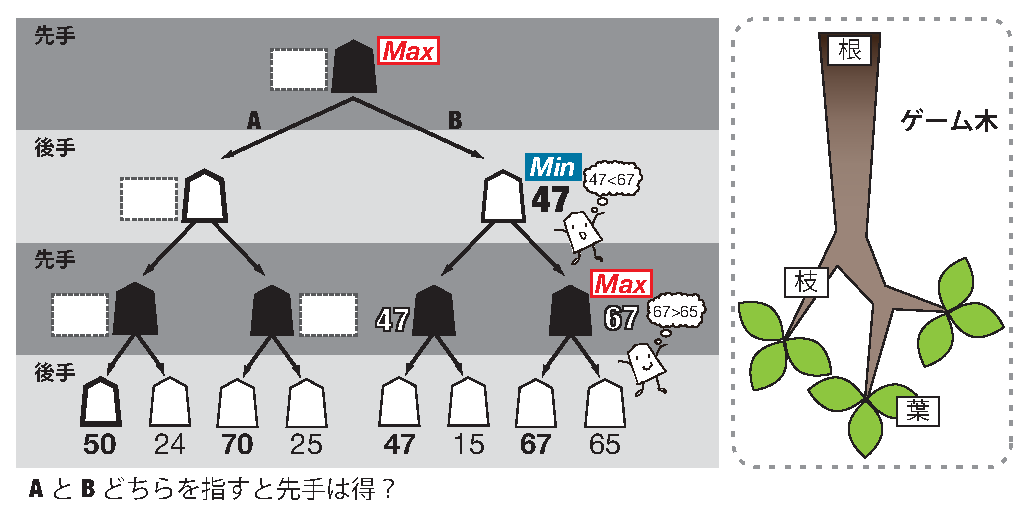
\includegraphics[width=0.9\linewidth]{gametreekr.eps}}


\begin{itemize}
\item min-max treeの説明\url{http://en.wikipedia.org/wiki/Minimax}
\item 解けている局面から前に戻る(Retrograde analysis, c.f., どうぶつしょうぎの完全解析)ことが適する場合と
\item 解きたい局面から先を調べる(探索+$\alpha-\beta$ pruning他)方が適切な場合がある.$\alpha-\beta$ pruningは最善手から順に読むと最大の効率を発揮し,探索節点数がすべて読む場合のsqrt程度になる.\url{http://en.wikipedia.org/wiki/Alpha
\end{itemize}

色々
\begin{itemize}
\item 局面の表現: 状態(局面)を小さく表現するとコピーが容易.幅優先,最
  良優先探索も可能.大きな表現を使う場合はglobalに一つ用意して
  makemove/unmake moveする.深さ優先探索のみ適する.必要ならiterative deepeningする.
\item 評価関数の作り方: 上記``House of Cards''のように数値の和を増やしてゆくようなゲームなら容易.オセロや将棋の評価関数は大量のデータから統計的に作るので,短いコンテストではたぶん出ない
\item 合流やループに注意: ほとんどのゲームでゲーム「木」は木ではない.
  合流を扱う場合は局面表(transposition table, 要はdp表)が必要.ループ
  はさらに話をややこしくする.特に履歴が勝敗に影響する場合(同一局面4回
  目で引き分けだが連続王手の繰り返しの場合は攻撃側が負けとか,囲碁の劫
  とか),局面表に勝敗を書き込む際に履歴の影響を検討しないと勝敗を誤る
  場合がある(GHI, graph
  history interaction問題).可能ならRetrograde analysisの方が無難.
\end{itemize}

その他:
\begin{itemize}
\item モンテカルロ木探索(MCTS, UCT) 短いコンテストではたぶん出ない? \url{http://en.wikipedia.org/wiki/Monte_Carlo_tree_search}
\item 証明数探索(proof-number search): 証明に必要そうなところから展開する最良優先探索の一種 \url{http://webdocs.cs.ualberta.ca/~mmueller/ps/ICGA2012PNS.pdf},
  \url{http://web.archive.org/web/20041204235835/http://www.cs.vu.nl/~victor/thesis.html}
\end{itemize}


\section{その他の問題}

\begin{pbox}[Ononokomachi's Edit War]
数式編集ゲーム  

\aojid{2512}
\end{pbox}

\begin{pbox}[Chat noir (UTPC 2009)]
猫が脱出できるか.
  
\aojid{2196}
\end{pbox}

\begin{pbox}[Game Strategy (世界大会 2014)]
AliceとBobのゲーム

\url{https://icpcarchive.ecs.baylor.edu/index.php?option=com_onlinejudge&Itemid=8&category=590&page=show_problem&problem=4785}
\end{pbox}

\begin{pbox}[Iyasugigappa]
Frog, Kappa and Weasel の3人(?)のゲーム.

\aojid{2557}
\end{pbox}

\begin{pbox}[Sweet War]
列の先頭のチョコを食べたりパスしたりする二人ゲームの勝敗.

\aojid{1353}
\end{pbox}

\begin{pbox}[Circular Game]
手番ごとに駒を動かして,動かせなくなったほうが負け.どちらが勝つか?

\url{http://main.edu.pl/en/archive/pa/2009/gra}
\end{pbox}

\begin{pbox}[Termites]
数値列が与えられる.AさんとBさんが交互にプレイして,数値列中0の隣のどれ
かの数値を自分の得点に加えその数値を0に変更する.お互い最適にプレイした場合の双方の得点を求めよ.

\url{http://main.edu.pl/en/archive/pa/2010/ter}
\end{pbox}

たぶんscanfの方が無難.

\end{versionalpha}

 % Commented out: Included file

\part{Appendix}

\begin{versionoutside}
\chapter{Conclusion}
If you notice any errors or areas for improvement in the document, please contact the author (kaneko@acm.org). We have received numerous comments and evaluations to date. Although I will refrain from expressing individual gratitude at this time, I would like to express my appreciation here.

The image illustrations in the document are borrowed from \url{https://openclipart.org/}, which are provided under the public domain, unless otherwise noted.

\vfill

\begin{itembox}[r]{-}
The author became aware of the existence of contest-style programming when an independent "study group" (which later became "Practical Programming" in the winter semester) was started by Associate Professor Masuhara (then) in the summer semester of 2004. Since then, the activities of the ACM-ICPC OB/OG Association, the exchange of technology on blogs, the publication of the Japanese online judge system (Aizu Online Judge), the holding of original contests at various universities, the publication of the Programming Contest Challenge Book, and the regular contests of atcoder, etc., have significantly increased the excitement of the Japanese participant community. Since the learning environment at a certain level or higher seems to be well-developed by now, we hope that it will develop further if we can improve the learning efficiency so that inexperienced people can reach an enjoyable level more quickly.
\end{itembox}
\end{versionoutside}


\appendix
%\chapter{Bugs and Debugging}\label{chapter:debug}

It would be ideal if a program worked exactly as intended the first time it was written, but that is often not the case. It takes only a moment to introduce a bug, but it can often take more than two hours to remove it. Furthermore, when using C or C++, the detection mechanisms and error messages for code that is not guaranteed to work are often unhelpful, which can make it take a long time to find the cause.
Familiarizing yourself with the useful tools available in the development environment may reduce the time spent investigating the cause.
Especially in programming contests, where both time and computer usage are limited, it is desirable for teams to determine efficient methods.

\section{Bug Prevention and Programming Practices}
Paradoxically, to reduce debugging time, it is effective to spend time preventing bugs from being introduced. One way to do this is to adopt good programming styles.
There are various books on this topic, so it is good to find one that suits you. Here are some examples.

\paragraph{Variable Usage} Using variables appropriately makes programs easier to read.

Bad Example: (Calculating the area of a circle where (x1, y1) and (x2, y2) are the endpoints of the diameter)
\begin{cbox}
double area = sqrt((x2-x1)*(x2-x1)+(y2-y1)*(y2-y1))/2
 * sqrt((x2-x1)*(x2-x1)+(y2-y1)*(y2-y1))/2 * 3.1415;\end{cbox}
Improved Example:
\begin{cbox}
double radius = sqrt((x2-x1)*(x2-x1)+(y2-y1)*(y2-y1))/2;
double area = radius*radius*3.1415;\end{cbox}
Why it's better:
\begin{itemize}
\setlength{\itemsep}{0pt}
\item Easier for humans to read (reduces the places to check if x1 is mistaken for x2)
\item No typing/copy-paste errors
\item Easier to grasp intermediate results (in this case, the radius). (Easy to display with a debugger or printf)
\end{itemize}

\paragraph{Function Usage} Similarly, it leads to more readable programs.
  \begin{cbox}
double square(double x) { return x*x; }
double norm(double x1, double y1, double x2, double y2) {
  return square(x2-x1)+ square(y2-y1);
}
double circle_area(double r) { return r*r*3.1415; }\end{cbox}
\paragraph{Constant Usage} Giving names to constants also improves readability.
  \begin{cbox}
const double pi = 3.1415;
const double pi = atan2(0.0,-1.0);    
\end{cbox}
\paragraph{Keep Variable Scope as Short as Possible}
The shorter the scope of a variable, the better. Relatedly, avoid reusing variables, and it is good to use one variable for only one purpose.
\begin{cbox}[emph={j}]
int i, j, k;
// Suppose there is a function that uses j or k around here
...
int main() {
  for (i=0; j<5; ++i) // Oh no!
    cout << "Hello, world" << endl;
  ...
}
\end{cbox}
Declaring the necessary variables for each function greatly improves the situation.
\begin{cbox}
int main() {
  int i;
  for (i=0; j<5; ++i) // Compilation error
    cout << "Hello, world" << endl;
}
\end{cbox}
However, in modern languages such as C++ and Java, you can declare variables used in loops within the for statement, so this is recommended.
\begin{cbox}
int main() {
  for (int i=0; i<5; ++i) 
    cout << "Hello, world" << endl;
}
\end{cbox}
\paragraph{Avoid Common Pitfalls} There are some things that are good to learn in advance.
    C Language FAQ \url{http://www.kouno.jp/home/c_faq/} Especially 16 Strange Problems
\paragraph{Understand Compiler Messages} Compilers sometimes give helpful advice. Do not ignore them.
  \begin{itemize}
  \item ``if-parenth.cc:8:14: warning: suggest parentheses around assignment used as truth value''
\begin{cbox}
  if (a = 1) return 1;
  if (a =! 1) cout << "ok";
\end{cbox}
\item ``no return statement in function returning non-void [-Wreturn-type]''
\begin{cbox}
int add(int a, int b) {
  a+b; // Correctly \cemph{return} a+b;
}
\end{cbox}
  \end{itemize}
\section{Debugging Tools}

\subsection{Tool: assert}

In major languages such as C, C++, Python, and Java, a mechanism called \tindex{assert} is provided for understanding programs and testing during execution.
The assert statement checks a conditional expression during program execution, and if it is true, does nothing; if it is false, it displays an error message and stops.

\paragraph{Code Example}
Calculation of factorial:
\begin{cbox}[emph={factorial}]
int factorial(int n) {
  if (n == 1)
    return 1;
  return n * factorial(n-1);
}
int main() {
  cout << factorial(3) << endl; // Outputs 3*2*1 = 6
  cout << factorial(-3) << endl; // If you accidentally enter a negative number, it won't stop
}
\end{cbox}

The above function works correctly only when the argument n is positive.
We want to ensure that the argument n is positive at runtime. To do this, include the cassert header and add an assert statement. As you can see, the content you want to guarantee is described as a conditional expression within the parentheses of assert.
\begin{cbox}[emph={cassert,assert}]
#include <cassert> // Added
int factorial(int n) {
  assert(n > 0); // Added
  if (n == 1)
    return 1;
  return n * factorial(n-1);
}
\end{cbox}

In this way, when writing a program based on some "premise," it is good to "assert" that in the source code for better clarity.

If you call \texttt{factorial(-1)} in this way, it will display an error and stop.

\begin{terminal}
Assertion failed: (n > 0), function factorial, file factorial.cc, line 3.
\end{terminal}

Since \texttt{assert} is a runtime test, it can cause a decrease in execution speed.
For this reason, a method is provided to easily disable all asserts without changing the source code.
For example, define the NDEBUG macro *before* including the cassert header, as follows:
\begin{cbox}[emph={NDEBUG}]
#ifndef NDEBUG
#  define NDEBUG
#endif
#include <cassert>
\end{cbox}

assert can also be used in Python. If you start with the option -O, such as \texttt{python3 -O}, the \texttt{assert} statement will be disabled.

\begin{pybox}[emph=assert]
def factorial(n):
    assert n >= 0
    if n == 0:
        return 1
    return n*factorial(n-1)
\end{pybox}

assert can also be used in Java.
\begin{javabox}[emph={Main,assert}]
public class Main {
    static int factorial(int n) {
	assert n >= 0;
	if (n == 0) return 1;
	return n*factorial(n-1);
    }
    public static void main(String[] args) {
	System.out.println(factorial(3));  // This will succeed
	System.out.println(factorial(-3)); // This will...
    }
}
\end{javabox}

In the case of Java, assert is enabled (only when it is added) by adding \texttt{-ea} as a runtime option.
\begin{terminal}
$ java -ea Main
6
Exception in thread "main" java.lang.AssertionError
	at Main.factorial(Main.java:3)
	at Main.main(Main.java:10)  
\end{terminal}
\subsection{Tool: -fsanitize}\label{section:cpp-sanitize}
In relatively new C++, compiler options such as \texttt{-fsanitize=undefined} and \texttt{-fsanitize=address} are available.
These options are useful when you have written an "incorrect program, but you don't know it, or you can't identify the location."

The function \texttt{fib} in the following program has a bug where it does not return a value when the argument \texttt{i==0}.
\begin{cbox}
#include <iostream>
using namespace std;
int fib(int i) {
  if (i == 1) return 1; // Forgot the case for i==0
  else if (i >= 2) return fib(i-1)+fib(i-2);
}
int main() {
  cout << fib(2) << endl;
}  
\end{cbox}

When the \texttt{-fsanitize=undefined} option is enabled as shown below, a runtime error is detected.
\begin{terminal}[emph={fsanitize,undefined}]
$ g++ -Wall fib.cc
$ ./a.out
2  
$ g++ -Wall -fsanitize=undefined fib.cc
$ ./a.out 
fib.cc:3:5: runtime error: execution reached the end of a value-returning function without returning a value
Abort trap: 6
\end{terminal}

The following (careless) program works correctly only when the integer read from the keyboard is between 0 and 3 inclusive.
\begin{cbox}
#include <iostream>
using namespace std;
int A[4] = {0,1,2,3};
int f(int idx) {
  return A[idx];
}
int main() {
  int idx;
  cin >> idx;
  cout << f(idx) << endl;
}
\end{cbox}

If you compile with \texttt{-fsanitize=undefined}, it will tell you that a violation occurred on line 5.
\begin{terminal}[emph={fsanitize,undefined}]
$ g++ -Wall -fsanitize=undefined test.cc
$ ./a.out 
|3|
3
$ ./a.out 
|8|
test.cc:5:10: runtime error: index 8 out of bounds for type 'int [4]'
\end{terminal}


\texttt{-fsanitize=undefined} is useful, but it is not a panacea.
Memory-related runtime errors can sometimes be found with \texttt{-fsanitize=address}.
The following program accesses an invalid address when \text{i=4}.
\begin{cbox}
#include <iostream>
using namespace std;
int A[4]={0,1,2,3};
int main() {
  int *p = A;
  for (int i=0; i<5; ++i) // 5 is a mistake for 4
    cout << *(p+i) << endl;
}  
\end{cbox}
Even if you use \texttt{-fsanitize=undefined}, this invalid memory access is not detected, and the program runs as if nothing happened.
\begin{terminal}[emph={fsanitize,undefined}]
$ g++ -Wall -fsanitize=undefined addr.cc 
$ ./a.out 
0
1
2
3
8842826
\end{terminal}

If you compile with \texttt{-fsanitize=address}, the invalid memory access is detected.
\begin{terminal}[emph={fsanitize,address}]
$ g++ -Wall -fsanitize=address addr.cc 
$ ./a.out 
0
1
2
3
=================================================================
==37898==ERROR: AddressSanitizer: global-buffer-overflow on address 0x000107f8d110 at pc 0x000107f8c8ea bp 0x7ffee7c74970 sp 0x7ffee7c74968
READ of size 4 at 0x000107f8d110 thread T0
    #0 0x107f8c8e9 in main (a.out:x86\_64+0x1000018e9)
    #1 0x7fff50332014 in start (libdyld.dylib:x86\_64+0x1014)
\end{terminal}
\subsection{Tool: \_GLIBCXX\_DEBUG (G++)}

In the case of G++, if you define \texttt{\_GLIBCXX\_DEBUG} at the beginning, it will find some mistakes.
(\url{http://gcc.gnu.org/onlinedocs/libstdc++/manual/debug_mode_using.html#debug_mode.using.mode})

\begin{cbox}[emph={_GLIBCXX_DEBUG}]
#define _GLIBCXX_DEBUG
#include <vector>
using namespace std;
int main() {
    vector<int> a;
    a[0] = 3; // Violation of assigning to a vector of length 0
}
\end{cbox}

Execution example: (Instead of simply causing a segmentation fault, it tells you that it is out-of-bounds)
\begin{terminal}
/usr/include/c++/4.x/debug/vector:xxx:error: attempt to subscript container 
    with out-of-bounds index 0, but container only holds 0 elements.
\end{terminal}

\subsection{Tool: gdb}

Suppose you accidentally write a for loop that doesn't stop, like this:
\begin{cbox}
int main() { // Intending to repeat "hello" and "world" with newlines
  for (int i=0; i<10; ++i) {
    for (int j=0; j<2; ++i)
      cout << "hello " << endl;
    cout << "world" << endl;
  }
}
\end{cbox}

To prepare to use gdb, add the \texttt{-g} option to the compilation options.
\begin{terminal}[emph={g}]
$ g++ -g -Wall filename.cc
\end{terminal}

When executing, start gdb by giving it the name of the program to be debugged, and type run inside gdb.
\begin{terminal}[emph={gdb,a.out,run,bt,up,list,p}]
$ gdb ./a.out
(gdb starts)
(gdb) run # (Normal execution)
(gdb) run < sample-input.txt # (When using redirection)
# ...(The program executes)...
# ...(Stop by typing Ctrl-C or due to a segmentation fault, etc.)
(gdb) bt
(gdb) up // Go up to main a few times
(gdb) up
#12 0x080486ed in main () at for.cc:6
6	      cout << "hello " << endl;
(gdb) list
1	#include <iostream>
2	using namespace std;
3	int main() {
4	  for (int i=0; i<10; ++i) {
5	    for (int j=0; j<2; ++i)
6	      cout << "hello " << endl;
7	    cout << "world" << endl;
8	  }
9	}
(gdb) p i
$1 = 18047
(gdb) p j
$2 = 0
\end{terminal}

Main commands:
\begin{itemize}
\setlength{\itemsep}{0pt}
\item Display function call relationships: bt
\item Display the value of a variable: p variable name
\item Move one level up (to the caller): u
\item Display source code: list
\item Step execution: n, s
\item Continue execution: c
\item Exit gdb: q
\end{itemize}

You can also set breakpoints to interrupt execution when a specific location in the source code is reached, or when a variable's value is changed. See the manual for details.

\subsection{Tool: valgrind}

\begin{cbox}
int main() {
    int p; // Forgot initialization
    printf("
}  
\end{cbox}

Compile with the \texttt{-g} option, as when using gdb.
\begin{terminal}[emph={g}]
$ g++ -g -Wall filename.cc
\end{terminal}

When executing, give the executable program to the valgrind command.

\begin{terminal}[emph={valgrind,a.out}]
$ valgrind ./a.out
Conditional jump or move depends on uninitialised value(s)
...
\end{terminal}

\section{Sampling: Once You've Identified the Cause of a Bug}

Once you've identified the cause of a bug, sampling it can be used as an asset to reduce future debugging time. If you move on with "I'm lucky it worked," nothing will remain. Although it's off-topic, even in situations where you get stuck due to overlooking problem constraints or misunderstanding the meaning of the text, it would be helpful to collect patterns of misreading.

Array Boundaries
\begin{cbox}
    int array[3];
    printf("
\end{cbox}

Uninitialized Variables
\begin{cbox}
    int array[3];
    int main() {
      int a;
      printf("
    }  
\end{cbox}

Function without return
\begin{cbox}
int add(int a, int b) {
  a+b; // Correctly \cemph{return} a+b;
}
int main() {
  int a=1,b=2;
  int c=add(a,b); // The value of c is undefined
}
\end{cbox}

Stack Overflow
\begin{cbox}
  int main() {
    int a[100000000]; // It's better to move this to a global variable
  }
\end{cbox}

Invalid Pointer
\begin{cbox}
int *p;
*p = 1;  

char a[100];
double *b = &a[1];
*b = 1.0;
\end{cbox}

Required capacity for strings: A null terminator '\textbackslash{}0' is needed at the end
\begin{cbox}  
    char a[3]="abc"; // Correctly a[4] = "abc" or a[] = "abc"
    printf("
\end{cbox}

% A[i] (i is in the range $[0,N-1]$) trying to display in reverse order
\begin{cbox}
for (unsigned int i=N-1; i>0; ++i)
  cout << A[i] << endl;
\end{cbox}


% Want to read two integers
\begin{purecbox}
int a, b;
scanf("
\end{purecbox}
\begin{cbox}
int a, b;
cin >> a, b;
\end{cbox}


\chapter{Understanding Programming Languages and Environments}
\section{Loop Invariants}\label{chapter:loop-invariants}

Let's consider the correctness of a simple \texttt{for} statement like the following:

\begin{terminal}[emph={}]
def name(parameter1, parameter2...):
    variable = initial_value
    for ...
      variable = expression # Rewrite the variable to a new value
    return variable
\end{terminal}

Consider the following example problem and its solution.

\begin{psbox}{Sum of Consecutive Numbers (sum\_to\_n)}{no judge}
  Create a function \texttt{sum\_to\_n(n)} that calculates the sum of integers from 1 to $n$ by naively adding them. Assume $1<n$.
  (Verify with n=10000, etc.)
\end{psbox}

Example Solution:
\begin{pybox}
def sum_to_n(n):
    sum = 0
    for i in range(1, n+1):
        sum = sum + i
    return sum
\end{pybox}
Let's trace how such a program is derived.

If we were to calculate the sum up to a fixed value of 3, it could be written simply.
\begin{pybox}
def sum3():
    return 1+2+3
\end{pybox}
Using auxiliary variables $s_i$ (the sum from 0 to i), we can rewrite it into an equivalent program.
\begin{pybox}
def sum3():
    s0 = 0 # Sum of an empty set
    s1 = s0 + 1 # Sum of 1
    s2 = s1 + 2 # Sum of 1 and 2
    s3 = s2 + 3 # Sum of 1, 2, and 3
    return s3
\end{pybox}

Using assignment, we can also express the auxiliary variables $s_i$ with a single variable \texttt{sum}.
\begin{pybox}
def sum3():
    sum = 0 # sum is equivalent to s0
    sum = sum + 1 # The sum on the left is equivalent to s1, the sum on the right is equivalent to s0
    sum = sum + 2
    sum = sum + 3
    return sum # sum is equivalent to s3
\end{pybox}
The \texttt{for} loop version of this is the example solution at the beginning.

\begin{pybox}[emph=sum]
def sum_to_n(n):
    sum = 0
    for i in range(1, n+1):
        # (a) At this point, the value of sum is the sum from 0 to i-1
        sum = sum + i  # Note that sum += i is the same
        # (b) At this point, the value of sum is the sum from 0 to i
    return sum
\end{pybox}
Please confirm that the conditions regarding the value of sum described in comments (a) and (b) hold true at any point in the loop. Such conditions are called \texttt{loop invariants}.
Using these conditions regarding the value of sum, we can prove that the function calculates the sum up to n.

\section{Recursion}\label{section:recursion}

\subsection{Inductive Definitions and Linear Recursion}\label{section:linear}

Consider the situation of "wanting to calculate something repeatedly." There are two ways to write this: one is by using iteration or \textbf{loops} such as \texttt{while} or \texttt{for}, and the other is by using \tindex{recursion} where a function calls itself. Here, we will delve into the latter.

As an example, let's define a function equivalent to $1+2+\cdots+n$ using a \tindex{recurrence relation}.
If we write this function as $\mbox{sum}(n)$, it can be defined inductively as follows:
\[
        \mbox{sum}(n) = \left\{
        \begin{array}[c]{ll}
          1 & \mbox{when $n=1$}\\
          n + \mbox{sum}(n-1) & \mbox{otherwise}
        \end{array}
      \right.
\]
Note that sum itself is used within this definition.
This can be almost directly translated into Python or C++ definitions:
\begin{cbox}[emph={sum}]
int sum(int n) {
  if (n == 1) return 1;
  else return n + sum(n-1);
}
\end{cbox}
\begin{textblock}{3}(4,-1.2)
\begin{shaded*}
\noindent
The \textcolor{ired}{sum} in red is the recursive structure.
\end{shaded*}
\end{textblock}
\begin{pybox}[emph={sum1}]
def sum1(n):
    if n == 1:
        return 1
    else:
        return n + sum1(n-1)
\end{pybox}

\paragraph{Understanding Program Correctness} It is good to confirm the following two points:
\begin{itemize}
\item Confirm the correctness of the base case: when $n=1$, \texttt{sum1(n)}$=1$
\item Assuming correctness up to $n-1$, confirm the correctness for $n$: \texttt{sum1(n)}$=n+$\texttt{sum1(n-1)}
\end{itemize}

\subsection{Recursion with Branching}\label{section:branching}
In the recursive calls we have seen so far, a function called itself only once. From now on, we will deal with cases where multiple recursive calls are made.


\begin{psbox}{Fibonacci Numbers}{no judge}
The Fibonacci sequence (\eindex{Fibonacci numbers}) is a sequence of numbers formed by "the sum of the previous two numbers," such as
\[
        0, 1, 1, 2, 3, 5, 8, 13, 21, \ldots
\]
Inductively define the $n$-th Fibonacci number $\mathit{fib}(n)$.
Also, define the function \texttt{fib(n)}.
\end{psbox}

\begin{pybox}
def fib(n):
    print("fib",n) # Display the argument when the function is called
    if n == 0:
        return 0
    elif n == 1:
        return 1
    else:
        return fib(n-2)+fib(n-1)
\end{pybox}

Note that recursion is not the best way to calculate Fibonacci numbers. More efficient ways to find Fibonacci numbers will be discussed separately.


\paragraph{Tail Recursion}

Consider the following definition of $\mbox{sum}'(s,n)$, which is a slight modification of the formula:
\[
        \mbox{sum}'(s,n) = \left\{
        \begin{array}[c]{ll}
          s+1 & \mbox{when $n=1$}\\
          \mbox{sum}'(s+n, n-1) & \mbox{otherwise}
        \end{array}
      \right.
\]
Considering $s$ in the above definition as "the sum so far," confirm that $\mbox{sum}(n) = \mbox{sum}'(0,n)$.


\begin{pybox}[emph={sum2}]
def sum2(s,n):
    if n == 1:
        return s+1
    else:
        return sum2(s+n, n-1)
\end{pybox}

A structure where a function calls itself as its return value is called \jindex{tail recursion}{tail recursion}. Writing it this way has the advantage that it is easier for the compiler to optimize.

Also, introducing auxiliary variables like $s$ can sometimes improve the clarity of recursion.





\begin{tipsbox}{maximum recursion depth exceeded}
Recursive functions must be implemented to stop somewhere. For example, the following function does not have a defined stopping point.
\begin{pybox}
def inf(a):
    return 1+inf(a)
\end{pybox}
If you call this function as \texttt{inf(0)},
\begin{terminal}[name=RecursionError]
>>> inf(0)
Traceback (most recent call last):
  File "<stdin>", line 1, in <module>
  File "<stdin>", line 2, in inf
  File "<stdin>", line 2, in inf
  File "<stdin>", line 2, in inf
  [Previous line repeated 995 more times]
RecursionError: maximum recursion depth exceeded
\end{terminal}
you will see an error message indicating that the process could not continue due to \texttt{RecursionError: maximum recursion depth exceeded}.

\end{tipsbox}

\medskip

\paragraph{Recursive Thinking about Operations}
As an example, consider the operation \texttt{print\_range(n)} that displays integers from 1 to n. Similar to the previous \texttt{sum}, the operation can be defined as follows:
\[
        \mbox{\cemph{print\_range}}(n) = \left\{
        \begin{array}[c]{ll}
          \text{Display } 1 & \mbox{when $n=1$}\\
          \mbox{\cemph{print\_range}}(n-1) \; \langle\text{afterward}\rangle
          \; \text{Display } n & \mbox{otherwise}
        \end{array}
      \right.
\]

\begin{pybox}[emph={print_range}]
def print_range(n):
  if n == 1:
    print(1)
  else:
    print_range(n-1)
    print(n)
\end{pybox}


\begin{psbox}{m-ary Numbers}{no judge}
  Given integers m and n ($1\le n \le
  8$, $1 < m \le 10$).
  Create a function \texttt{mdigit(m,n)} that displays all n-digit m-ary numbers in ascending order.
\end{psbox}

\begin{terminal}
>>> mdigit(3,2)
00
01
02
10
11
12
20
21
22
\end{terminal}

For simplicity, consider $m=2$, i.e., binary numbers. For a positive integer $n$, we want to construct a procedure that achieves the goal based on a procedure that performs the same process for $n-1$.
In other words, assuming someone has created a function that displays all $n-1$ digit binary numbers (*1), can we create a function that displays all $n$ digit $m$-ary numbers based on that?

An $n$-digit binary number can be decomposed into the leftmost digit ($0$ or $1$) and the remaining $n-1$ digits.
Therefore, we want to do something like: display all $n-1$ digit binary numbers with \emph{0 added to the left}, and display all $n-1$ digit binary numbers with \emph{1 added to the left}.

Based on the above, by slightly adjusting the function (*1), add the string prefix that you want to be written on the left as an argument, and let \texttt{B}(prefix, n) be a function that "generates all n-digit binary numbers for the argument prefix and n, and displays each with the prefix attached."

\begin{equation}
  \texttt{B}(\text{prefix},n) = \left\{
  \begin{array}{ll}
    \text{Display prefix} & (n=0)\\
    \text{Execute } \texttt{B}(\text{prefix} + 0, n-1) \text{ and}\\
    \texttt{ B}(\text{prefix} + 1, n-1) & (n>1)
  \end{array}\right.\label{eq:rec-mn}
\end{equation}

\begin{center}
  \newcolumntype{G}{>{\columncolor[gray]{0.8}}c}
  \newcommand{\gr}[1]{\textcolor{gray}{#1}}
  \begin{tabular}{ll}
    \begin{minipage}{.4\linewidth}
      \begin{tabular}{Gcc}
        \multicolumn{1}{c}{prefix} & 3 & 2,1\\\hline
  10&0&\tikzmark{recmn0}\cellcolor{blue!10}00\\
  \gr{10}&\gr{0}&\cellcolor{blue!10}01\\
  \gr{10}&\gr{0}&\cellcolor{blue!10}10\\
  \gr{10}&\gr{0}&\cellcolor{blue!10}11\\\hdashline
  \gr{10}&1&\tikzmark{recmn1}\cellcolor{green!10}00\\
  \gr{10}&\gr{1} &\cellcolor{green!10}01\\
  \gr{10}&\gr{1} &\cellcolor{green!10}10\\
  \gr{10}&\gr{1} &\cellcolor{green!10}11
\end{tabular}
    \end{minipage}
    &
    \begin{minipage}{.2\linewidth}
\begin{tikzpicture}[remember picture,overlay]
\draw [dotted] (pic cs:recmn1) rectangle (pic cs:recmn1)+(1em,.7ex);


\draw[<-] ([xshift=2em]pic cs:recmn0) -- ++(0:5em) coordinate (aux0);
\node[right] at (aux0) {Realized through B(100,2)};

\draw[<-] ([xshift=2em]pic cs:recmn1) -- ++(0:5em) coordinate (aux1);
\node[right] at (aux1) {Realized through B(101,2)};

\end{tikzpicture}
    \end{minipage}
  \end{tabular}\\
\texttt{Operation of B(10,3): B(100,2) and B(101,2)}
\end{center}


Confirm that \texttt{B(0,n)} displays all $n$-digit binary numbers. To handle not only binary numbers but also $m$-ary numbers, the part that was branching only with $0$ and $1$ should be branched from $0$ to $m-1$ using a \texttt{for} statement or similar.

Although the prefix was explained assuming a string (\texttt{str}), it can also be represented with \texttt{int}. In that case, for example, the operation of adding 1 to the right of the prefix would be \texttt{prefix*10+1}.

Syntax: In Python, to display an integer a with N digits, padding with 0s when the number of digits is insufficient, do the following:
\begin{pybox}
>>> print("{:05d}".format(3))
00003
\end{pybox}
\subsection{Function and Execution State Management}\label{section:stackframe}

Let's supplement the "relationship between statements being executed from top to bottom and recursive calls."

\paragraph{Normal Function Call Case}

Although somewhat contrived, let's assume there is the following source code. When the function \texttt{helloworld} is executed, \texttt{hello} and \texttt{world} are displayed line by line.
\begin{pybox}
def mynewline():
    print("")

def myprint(msg): # Writes a message and adds a newline
    print(msg, end="")
    mynewline()

def helloworld():
    myprint("hello")
    myprint("world")
\end{pybox}

A schematic representation of a part of this execution process is as follows.
In many programming languages, including C++, when a function is called, a \tindex{frame} is created to manage the execution state and local variables of that function. In the figure below, frames are represented by boxes.

\begin{tabular}{lll}
  \begin{minipage}{.3\linewidth}
  \begin{itembox}[l]{helloworld()}
    \begin{alltt}
myprint("hello")\tikzmark{callhello}
myprint("world")\tikzmark{callworld}
\end{alltt}
  \end{itembox}
  \end{minipage}
&
  \begin{minipage}{.3\linewidth}
  \begin{itembox}[l]{\tikzmark{hello}myprint(msg=hello)}
    \begin{alltt}
print(msg, end="")
\tikzmark{mpend}mynewline()\tikzmark{callnl}
\end{alltt}
  \end{itembox}
  \end{minipage}
&
  \begin{minipage}{.3\linewidth}
  \begin{itembox}[l]{\tikzmark{nl}mynewline()}
    \begin{alltt}
\tikzmark{nlend}print("")
\end{alltt}
  \end{itembox}
  \end{minipage}
\\
&
  \begin{minipage}{.3\linewidth}
  \begin{itembox}[l]{\tikzmark{world}myprint(msg=world)}
    \begin{alltt}
print(msg, end="")
mynewline()
\end{alltt}
  \end{itembox}
  \end{minipage}
&
\end{tabular}

\begin{tikzpicture}[remember picture]
\draw[->,overlay,ultra thick,iblue,bend left=20,yshift=5](pic cs:callhello) to node[above,iblue] {(1)} (pic cs:hello);
\draw[->,overlay,ultra thick,iblue,bend left=20,yshift=5](pic
cs:callnl) to node[left,iblue] {(2)} (pic cs:nl);
\draw[->,overlay,ultra thick,dotted,iblue,bend left=20,yshift=-5](pic cs:nlend) to node[above,iblue] {(3)} (pic cs:callnl);
\draw[->,overlay,ultra thick,dotted,iblue,yshift=-5](pic cs:mpend) to node[above left,iblue] {(4)} (pic cs:callhello);
\draw[->,overlay,ultra thick,iblue,bend right=20](pic cs:callworld) to node[below,iblue] {(5)} (pic cs:world);
\end{tikzpicture}

When viewed within each frame, statements are executed in the order they are written. For example, in the leftmost \texttt{helloworld} frame, the execution of \texttt{myprint("hello")} is completed before the execution of \texttt{myprint("world")} begins.
The completion of the execution of \texttt{myprint("hello")} means that the call to the \texttt{myprint} function is executed (arrow (1)), and within that frame, the execution of all statements is completed and control is returned (arrow (4)). In that process, the \texttt{mynewline} function is also executed (arrows (2), (3)).
As shown by arrows (3) and (4), when the execution of all statements in a frame is completed or a \texttt{return} occurs, control is returned to the appropriate location in the caller.

\paragraph{Recursive Case} Similarly, in the case of recursion, a frame is created for each call.
Suppose the m-ary number example from Section \ref{section:branching} is implemented as follows:

\begin{pybox}[emph={B}]
def B(prefix, n):
    if (n==0):
        ...
        return
    B(prefix+"0", n-1)
    B(prefix+"1", n-1)
\end{pybox}

At this time, the call to \texttt{B("",3)} proceeds as follows:

\begin{tabular}{@{}llll@{}}
  \begin{minipage}{.2\linewidth}
  \begin{itembox}[l]{B("", n=3)}
    \begin{alltt}
B(""+"0",2)\tikzmark{callB02}
B(""+"1",2)
\end{alltt}
  \end{itembox}
  \end{minipage}
&
  \begin{minipage}{.21\linewidth}
  \begin{itembox}[l]{\tikzmark{B02}B("0", n=2)}
    \begin{alltt}
B("0"+"0",1)\tikzmark{callB001}
B("0"+"1",1)
\end{alltt}
  \end{itembox}
  \end{minipage}
&
  \begin{minipage}{.23\linewidth}
  \begin{itembox}[l]{\tikzmark{B001}B("00", n=1)}
    \begin{alltt}
B("00"+"0",0)\tikzmark{callB0000}
B("00"+"1",0)\tikzmark{callB0010}
\end{alltt}
  \end{itembox}
  \end{minipage}
&
  \begin{minipage}{.23\linewidth}
  \begin{itembox}[l]{\tikzmark{B0000}B("000", n=0)}
    \begin{alltt}
\tikzmark{B0000end}if (n==0) ...
\end{alltt}
  \end{itembox}
  \begin{itembox}[l]{\tikzmark{B0010}B("001", n=0)}
    \begin{alltt}
if (n==0) ...
\end{alltt}
  \end{itembox}
  \end{minipage}
\end{tabular}

\begin{tikzpicture}[remember picture]
\draw[->,overlay,ultra thick,iblue,bend left=20,yshift=5](pic cs:callB02) to node[above,iblue] {(1)} (pic cs:B02);
\draw[->,overlay,ultra thick,iblue,bend left=20,yshift=5](pic
cs:callB001) to node[above,iblue] {(2)} (pic cs:B001);
\draw[->,overlay,ultra thick,iblue,bend left=20,yshift=5](pic
cs:callB0000) to node[above,iblue] {(3)} (pic cs:B0000);
\draw[->,overlay,ultra thick,dotted,iblue,yshift=-5](pic
cs:B0000end) to node[above,iblue] {(4)} (pic cs:callB0000);
\draw[->,overlay,ultra thick,iblue,bend right=20,yshift=5](pic
cs:callB0010) to node[below,iblue] {(5)} (pic cs:B0010);
\end{tikzpicture}

Note that even if it is the same function in the source code, a different frame is created for each call.
Each frame maintains information such as arguments, local variables, and how far the execution has progressed.
A \tindex{stack area} is used to manage such information (different from the stack data structure).
Frames that have completed execution are discarded, but frames that have not completed need to be maintained in memory. Therefore, calling a function many times (e.g., 1 million times) may result in a runtime error. For example, in the standard exercise environment, the limit is 8 megabytes. \index{ulimit}
\begin{terminal}
ssh0-01m:~ 0123456789$ ulimit -a
...
stack size              (kbytes, -s) 8192
...
\end{terminal}
\section{Understanding Integer Types}\label{section:long-long}

In this material, we will use the \texttt{int} and \texttt{long long} types as needed to represent integers. There is a difference in the range of numbers that can be represented by each.

\begin{cbox}
    long long a = 1000000;
    int b = 1000000;
    cout << a * a << endl; // 1000000000000
    cout << b * b << endl; // -727379968 (overflow)
\end{cbox}

Usually, in C++, integers are represented by variables of type \texttt{int}. However, in the iMac environment of this exercise, as shown in Table \ref{table:nlimits}, the range of values that can be represented by the \texttt{int} type and other integer types is limited.

In the previous example,
$$1\,000\,000 \cdot 1\,000\,000 = 10^{12} > 2^{31} \approx 2\cdot10^{9}$$
exceeds the range that can be represented by a 32-bit integer.
Therefore, in such cases, it is necessary to use the \eindex{long long} type. One of the goals is to be able to grasp this \cemph{before starting to write the program}. \footnote{It is recommended to memorize $2^{10}=1\,024\approx10^3$ in order to perform such calculations smoothly.}

\begin{table}
  \centering
  \caption{Representation of signed integers in the environment assumed by this material}
  \label{table:nlimits}
  \begin{tabular}{l|rrrl}\hline
    type & bits & Lower Limit & Upper Limit & Notes\\\hline
    \cemphtt{int} & $32$ & $-2^{31}$ & $2^{31}-1$ & Approximately 2 billion\\
    \texttt{long} & $32/64$ & & & Not recommended for use\\
    \cemphtt{long long} & $64$ & $-2^{63}$ & $2^{63}-1$ & Standard type since C++11, previously a gcc extension\\
    \texttt{\_\_int128\_t} & 128 & & & gcc extension, not portable but powerful\\\hline
  \end{tabular}
\end{table}

The range that can be represented by each type may vary depending on the environment. You can check the environment you are using with the following program. The syntax of \texttt{numeric\_limits} is omitted, but those who are interested should investigate template classes and standard libraries \cite{book:cpp}.
\begin{cbox}[emph={limits}]
#include <limits>
#include <iostream>
using namespace std;
int main() {
  cout << sizeof(int) // Number of bytes
       <<' '<< numeric_limits<int>::digits // Number of bits excluding sign
       <<' '<< numeric_limits<int>::digits10 // Number of decimal digits
       <<' '<< numeric_limits<int>::min()
       <<' '<< numeric_limits<int>::max()
       << endl;
  cout << sizeof(long long)
       <<' '<< numeric_limits<long long>::digits
       <<' '<< numeric_limits<long long>::digits10
       <<' '<< numeric_limits<long long>::min()
       <<' '<< numeric_limits<long long>::max()
       << endl;
}  
\end{cbox}
\begin{terminal}
$ ./a.out
4 31 9 -2147483648 2147483647
8 63 18 -9223372036854775808 9223372036854775807  
\end{terminal}

Note that Table \ref{table:nlimits} only lists \jindex{signed integers}{signed integers}. \jindex{Unsigned integers}{unsigned integers} (\tindex{unsigned}\texttt{ int}, \texttt{unsigned long long}, etc.) cannot represent negative numbers, but can represent positive numbers in a range about twice as large. Although they are hardly used in this material, please understand them as needed.
In C++11, by using \texttt{\#include<cstdint>}, types such as \eindex{int32\_t} and \eindex{int64\_t} can be used. In the future, these should be used, but in this material, we will use \texttt{int} and \texttt{long long}.
\section{Floating-Point Numbers and Errors}\label{section:floating-point-numbers}

When dealing with real numbers, floating-point numbers are usually used.

However, depending on the situation, it may be appropriate to use integers to represent decimal numbers. For example, if you only need to handle up to two decimal places (like yen and sen), you can multiply the number by 100 to make it an integer. In that case, you can perform calculations internally as integers and only convert to decimal notation when displaying, such as with \texttt{cout << x/100 << "." << (x\%100) << endl;}. (Fixed-point)

To flexibly represent larger or smaller numbers, a real number representation (floating-point representation) with a \emph{sign part}, an \emph{exponent part}, and a \emph{mantissa part} is used.

\subsection{Various Errors}
When using floating-point numbers, it is necessary to understand that they involve errors.

Errors are not always intuitive.
As an example, consider a loop that processes from 0 to 1 in increments of 0.1.
In this case, the appropriate method is to use an integer for the loop counter. Even if they seem equivalent, the method of adding 0.1 each time can lead to unexpected results.

\begin{center}
\begin{tabular}{ll}\hline
  \begin{minipage}{.4\linewidth}
Good Implementation
\begin{pybox}
i = 0
while i < 10:
  print(i/10.0)
  i += 1
\end{pybox}    
  \end{minipage}
  &
  \begin{minipage}{.5\linewidth}
\begin{alltt}
0.0
0.1
(omitted)
0.8
0.9  # Total of 10 lines
\end{alltt}
  \end{minipage}
  \\\hline
  \begin{minipage}{.4\linewidth}
Bad Implementation
(Displays 11 lines from 0.1...)
\begin{pybox}
i = 0.0
while i < 1.0:
  print(i)
  i += 0.1
\end{pybox}
  \end{minipage}
  &
  \begin{minipage}{.5\linewidth}
\begin{alltt}
0.0
0.1
(omitted)
0.7999999999999999
0.8999999999999999
0.9999999999999999     # Total of 11 lines
\end{alltt}
  \end{minipage}
\\\hline\end{tabular}
\end{center}

Such phenomena arise from rounding errors, which will be explained next.
Furthermore, errors can increase in operations between numbers that already contain errors. There are four types of errors, classified as follows:

\begin{description}
\item[Round-off errors] Errors caused by the fact that decimal numbers can only be represented approximately with a finite number of digits when expressed in binary (equivalent to the fact that 1/3 cannot be accurately represented with a finite number of digits in decimal notation).
  \\
  Example: $0.1_{(10)} = 2^{-4} + 2^{-5}+2^{-8}+2^{-9}\ldots =
  1.10011\ldots_{(2)}\cdot 2^{-4}$\\
  Exercise: Predict the output of the following program?
  \begin{cbox}
#include <iostream>
using namespace std;
int main() {
  double a = 0.1;
  double b = 0.3;
  if (a*3 == b) cout << "OK" << endl;
  else cout << "NG" << endl;
}    
  \end{cbox}
  \begin{terminal}
0.1*3 = 0011111111010011001100110011001100110011001100110011001100110100
  0.3 = 0011111111010011001100110011001100110011001100110011001100110011    
  \end{terminal}
\item[Loss of significance] When taking the difference between two nearly identical numbers \emph{represented with a finite number of significant digits}, the number of significant digits decreases.
  \\
  Example: $0.124 - 0.123 = 0.001$\\
Note: This does not occur in operations between numbers that are originally represented without error.
\item[Information loss] In addition or subtraction of numbers with different magnitudes, the smaller number is ignored because it falls outside the significant range of the larger number.
  \\
  Example: $0.124 + 0.0000000123 = 0.124$
\item[Truncation errors] When numerically calculating the value of a function using an infinite series, errors occur due to approximating by truncating at a finite number of terms.
\end{description}

\subsection{Understanding the \texttt{double} Type}
In IEEE 754 double-precision (64-bit) floating-point format, a number is represented by a combination of three integers: the sign part $s$, the exponent part $e$, and the mantissa part $m$, as follows:
\begin{equation}
(-1)^s (1+m \cdot 2^{-52})) \cdot 2^{(e-1023)}.\label{eq:ieee64}
\end{equation}
The entire representation uses 64 bits, with the sign part $s$ occupying bit 0, the exponent part $e$ occupying bits 1-11 (11 bits), and the mantissa part $m$ occupying bits 12-63 (52 bits).

The following program uses the \texttt{union} feature to display the internal representation of a \texttt{double} type. Note that \texttt{bitset} is used here only to obtain the binary representation of an integer.

\begin{cbox}
#include <iostream>
#include <bitset>
using namespace std;
union double_long_long {
  double floating_value;
  unsigned long long integer_value;
};
void show_double(double v) {
  double_long_long u;
  u.floating_value = v;
  cout << v << " = " << bitset<64>(u.integer_value) << endl;
  long long sign = u.integer_value >> 63;
  long long exponent = (u.integer_value >> 52)& ((1<<11)-1);
  long long mantissa = u.integer_value & ((1ul<<52)-1);
  cout << " sign = " << sign << endl;
  cout << " exponent = " << exponent << ' ' << bitset<11>(exponent) << endl;
  cout << " mantissa = " << bitset<52>(mantissa) << endl;
  cout << " => " << (sign ? "-" : "+")
       << " (1+" << (double)mantissa/(1ul<<52)
       << ") * " << "2^(" << (exponent-1023) << ")" << endl;
}
int main() {
  show_double(1.0);
  show_double(-1.0);
  show_double(0.5);
  show_double(0.25);
  show_double(0.75);
}
\end{cbox}

Execution Example: Verify against Equation \ref{eq:ieee64}.
\begin{terminal}
1 = 0011111111110000000000000000000000000000000000000000(omitted)
 sign = 0
 exponent = 1023 01111111111
 mantissa = 000000000000000000000000000000000000000000(omitted)
 => + (1+0) * 2^(0)
-1 = 101111111111000000000000000000000000000000000000000(omitted)
 sign = 1
 exponent = 1023 01111111111
 mantissa = 000000000000000000000000000000000000000000(omitted)
 => - (1+0) * 2^(0)
0.5 = 00111111111000000000000000000000000000000000000000(omitted)
 sign = 0
 exponent = 1022 01111111110
 mantissa = 000000000000000000000000000000000000000000(omitted)
 => + (1+0) * 2^(-1)
0.25 = 0011111111010000000000000000000000000000000000000(omitted)
 sign = 0
 exponent = 1021 01111111101
 mantissa = 000000000000000000000000000000000000000000(omitted)
 => + (1+0) * 2^(-2)
0.75 = 0011111111101000000000000000000000000000000000000(omitted)
 sign = 0
 exponent = 1022 01111111110
 mantissa = 100000000000000000000000000(omitted)
 => + (1+0.5) * 2^(-1)
\end{terminal}

Exercise: Predict the bit string when 0.875 ($1/2+1/4+1/8$) is represented as a \texttt{double}. Verify using the program above.
\section{Structures: struct}\label{section:struct}

The \tindex{struct} is used to manage data collectively. With the following syntax, a new type called \texttt{Student} with integer variables \texttt{height} and \texttt{weight} is defined:
\begin{cbox}[emph=Student]
struct Student {
  int height, weight;
};
\end{cbox}

Example of use:
\begin{cbox}[emph=Student]
  Student a;
  a.height = 150;
  a.weight = 50;
  cout << a.height << ' ' << a.weight << endl;

  Student b = { 170, 70 };
  cout << b.height << ' ' << b.weight << endl;

  Student c = { 180 }; // weight == 0
  Student d = { };  // height, weight == 0
\end{cbox}
\begin{itemize}
\item To access the \texttt{height} or \texttt{weight} of each variable of type Student (in the above, \texttt{a, b, c, d}), use the \texttt{.} (dot) operator.
\item Initialization can also be done with curly braces \texttt{\{\}}.
\end{itemize}

\chapter{Ruby}\label{chapter:ruby}

\section{Input and Output}
This section mainly introduces sample code related to Chapter \ref{chapter:io}.

\subsection{ICPC Score Totalizer Software}
\begin{rbox}
while true
  judges = gets.to_i # Input a number
  break if judges == 0
  a = [] 
  for i in 0..judges-1
    a << gets.to_i
  end # By this point, the scores of each judge are in array a
  sum = 0
  for i in 0..judges-1
    sum = sum + a[i]
  end
  puts sum
  puts a.max
end
\end{rbox}

\subsection{Array Operations}

\begin{rbox}[emph={Array}]
  n = 50
  # Prepare an array of length n and initialize each element to 0 (valid from a[0] to a[n-1])
  a = Array.new(n,0)
\end{rbox}


\begin{rbox}[emph={each}]
a = Array.new(5)
a.each{|e| puts e}
\end{rbox}

\begin{rbox}
a = [3,5,1,2,4]
a.sort!
a.reverse! # Reverse the order of a
p a
\end{rbox}

\begin{rbox}
a = [0,1,2,3,4,5,6]
a[0,7] = a[3,4]+a[0,3]
p a # \dingright{} [3, 4, 5, 6, 0, 1, 2]
\end{rbox}

\subsection{Hanafuda Shuffle}
\begin{rbox}
while line = gets
  n, r = line.split(" ").map{|i| i.to_i} # Read n and r
  break if n == 0
  # Create a deck of n cards
  # Try displaying the created deck
  r.times {
    p, c = gets.split(" ").map{|i| i.to_i}
    # Perform shuffle p, c
    # Try displaying the entire deck after each shuffle
  }
  # Output the top of the deck
end
\end{rbox}

\section{Sorting and Greedy Algorithms}
This section mainly introduces sample code related to Chapter \ref{chapter:greedy}.

\subsection{Sorting}
\begin{rbox}
a = [3,5,1,2,4]
a.sort!
p a
\end{rbox}
\subsection{Finding Minimum String}

\begin{rbox}
N = gets.to_i
A = []
(1..N).each {
  A << gets.chomp 
}
... // Sort A as with integers
puts A[0]
\end{rbox}
\subsection{Pairs and Sorting}

\begin{rbox}
a = [3,5]
p a # Displays [3,5]
b = [0.5,"X"]
p b # Displays [0.5,"X"]
\end{rbox}

\subsection{Princess's Marriage}
\begin{rbox}
while line = gets
  pN, pM = line.split(" ").map{|s| s.to_i}
  break if pN == 0
  pd = [] # Array to store <p,d>
  (1..pN).each { # Do something pN times
    d, p = gets.split(" ").map{|s| s.to_i}
    pd << [p, d] 
  }
  # Try sorting pd in descending order
  # Try outputting pd
  # If the sorting is successful, try calculating the answer
end  
\end{rbox}

\section{Dynamic Programming}
This section mainly introduces sample code related to Chapter \ref{chapter:dp}.

\subsection{Naive Calculation of Fibonacci Numbers}
\begin{rbox}
def fib(n) # Slow version
  # p ["fib",n] Display the argument when the function is called
  if n==0
    0
  elsif n == 1
    1
  else
    fib(n-2)+fib(n-1)
  end
end  
\end{rbox}

\subsection{Heian-kyo Walking}

Input Example
\begin{rbox}
dataset = gets.to_i
dataset.times {
  gx, gy = gets.split(" ").map(&:to_i)
  p [gx,gy]
  matatabi = gets.to_i
  # In the problem statement, variable p is used, but it is separated from the display command p
  (0..matatabi-1).each{|i|
    x1,y1, x2,y2 = gets.split(" ").map(&:to_i)
    p [x1,y1, x2,y2]
  }
}  
\end{rbox}

\section{Basic Data Structures}
This section mainly introduces sample code related to Chapter \ref{chapter:datastructure}.

\subsection{Strings and Reading}
\begin{rbox}
word = gets.chomp # Reads a line with gets and removes the newline character at the end with chomp
puts word+word # Displays the concatenated string
\end{rbox}

\subsection{Stack}

In Ruby, we will use \texttt{unshift, shift} as \texttt{push, pop} respectively.
\begin{rbox}[emph={unshift,shift}]
stack = [] # (Treating an array as a Stack)
stack.unshift(3) # Add an element to the beginning
stack.unshift(4)
stack.unshift(1)
while stack.size > 0 # While there are elements
  n = stack.shift # Remove from the beginning
  p n
end  
\end{rbox}


In Ruby, it is convenient to treat an array as a queue.
\begin{rbox}[emph={shift}]
Q = [] # (Treating an array as a Queue)
Q << 3 # Add an element to the end
Q << 4
Q << 1
while Q.size > 0 # While there are elements
  n = Q.shift # Remove from the beginning
  p n
end
# 3, 4, 1 are displayed in this order
\end{rbox}

\subsection{Priority Queue}

In the case of Ruby, it seems that there are currently no libraries available for online judges, so it is necessary to implement a binary heap or similar yourself.
\begin{rbox}[emph={PriorityQueue,push,pop,size}]
class PriorityQueue
  def initialize
    # Implement a binary tree with an array. The left child of the i-th element is 2i+1, and the right child is 2i+2.
    # The parent element is assumed to have a higher priority than either of its children.
    @array = [] 
    @size = 0
  end
  def push(a)
    # After temporarily placing it at the end, move it up if its priority is higher than its ancestors.
    @array[@size] = a
    heapify_up(@size)
    @size += 1
  end
  def pop()
    # After taking out the root element (highest priority), temporarily place the last element at the root and adjust.
    raise unless @size > 0
    ans = @array[0]
    @size -= 1
    @array[0] = @array[@size]
    heapify_down(0)
    ans
  end
  def size
    @size
  end
  def swap(p,q) 
    @array[p],  @array[q] = @array[q], @array[p]
  end
  def equal_or_better(p,q)
    (@array[p] <=> @array[q]) <= 0
  end
  def heapify_up(n)
    while n > 0
      parent = (n-1)/2
      break if equal_or_better(parent, n)
      swap(parent,n)
      n = parent
    end
  end
  def heapify_down(n)
    while true
      l, r = n*2+1, n*2+2
      break if @size <= l
      child = l
      child = r if r < @size && equal_or_better(r, l)
      break if equal_or_better(n, child)
      swap(child, n)
      n = child
    end
  end
end

Q = PriorityQueue.new
Q.push([50, 1]);
Q.push([20, 2]);
Q.push([30, 3]);
Q.push([10, 4]);
Q.push([80, 5]);

while Q.size() > 0
  cur = Q.pop(); # Extract the smallest element
  p cur
end
\end{rbox}
\subsection{Strings and Splitting, Joining, Reversing}

\begin{rbox}
word = "hello"
s = word.split("")
(0..s.length).each {|l|
  a = s.first(l)
  b = s.last(s.length-l)
  # p a
  # p b
  puts a.join("")+" "+b.join("")
}  
\end{rbox}

\begin{rbox}
a = "hello"
b = a.reverse
puts b
\end{rbox}

\subsection{Sets}

In Ruby, you can achieve similar functionality using \texttt{Hash}.\footnote{Sets are also available, and you can use them by writing \texttt{require 'set'}, so those who are interested should investigate.}
For insertion, use \texttt{a[element]=1} instead of \texttt{a.insert(element)}; for the number or presence of a specified element, use \texttt{a[element]} instead of \texttt{a.count(element)}; and for the number of elements in the set, use \texttt{a.length} instead of \texttt{a.size()}.

\begin{rbox}
all = Hash.new(0)
puts all.length # 0
all["hello"] = 1
all["world"] = 1
all["good morning"] = 1
all["world"] = 1
puts all["world"] # 1
puts all["hello!!!"] # 0
puts all.length # 3
\end{rbox}

\subsection{Associative Arrays}

\begin{rbox}[emph={Hash}]
table = Hash.new(0) # Specified the value to be 0 when the key does not exist (*)
table["taro"] = 180
table["hanako"] = 160
puts table["taro"] # 180
puts table["ichirou"] # 0 (*)
\end{rbox}

\begin{rbox}
table["ichirou"] += 1
puts table["ichirou"] # 1
table["ichirou"] += 1
puts table["ichirou"] # 2
\end{rbox}


\begin{rbox}
phone = Hash.new
phone["taro"] = 123;
phone["jiro"] = 456;
phone["saburo"] = 789;

phone.each{|key,value|
  p [key, value]
}
# ["taro", 123]
# ["jiro", 456]
# ["saburo", 789]
\end{rbox}

In the case of Ruby, a more concise notation than C++ is possible. Specify the variables you want to use in the loop in the \texttt{|key,value|} part.

\section{Graph Traversal}
This section mainly introduces sample code related to Chapter \ref{section:graphsearch}.

Reading an Adjacency List (Example Graph)
\begin{rbox}
N = gets.to_i
G = (1..N).map{ Array.new(N, 0) }
N.times{
  u,k,*v = gets.split(' ').map(&:to_i) # u,k are numbers, v is an array
  v.each {|vi| # For each element vi in v
    # Connect (u-1) and (vi-1)
  }
}
G.each{|r|
  puts r.join(' ')
}
\end{rbox}

Breadth-First Search (BFS) (Chapter \ref{section:bfs})
\begin{rbox}
Q = [0] # Queue (array) with starting point 0
D = Array.new(N,-1)
D[0] = 0 # Distance to the starting point is 0, other distances are -1
while Q.size > 0
  p ["debug", Q] # Check the operation of Q at each step (remove later)
  cur = Q.shift
  (0..N-1).each {|dst|
    if ... then # If it is possible to move from cur to dst, and dst is unvisited \label{code:dfsruby:visit}
      D[dst] = D[cur]+1
      Q << dst # Push dst onto Q
    end
  }
end
# Display D
\end{rbox}

Depth-First Search (DFS) (Chapter \ref{section:dfs})
\begin{rbox}[emph={dfs}]
def dfs(src)
  D[src] = $time # Record the visit time
  $time += 1
  (0..N-1).each {|dst|
    if ... then # If it is possible to move from src to dst, and dst is unvisited
      dfs(dst)
    end
  }
  F[src] = $time # Record the finish time
  $time += 1
  # At the end of the function, \textcolor{iblue}{\textbf{return to the parent (blue arrow)}}
end


D = Array.new(N) # Initial value of D[i] is nil
F = Array.new(N)
$time = 1

(0..N-1).each {|id| # From the node with the smallest number
  if ! D[id] then # If D[id] is unvisited
    dfs(id) # Start dfs
  end
}
# Output
\end{rbox}

\section{Shortest Paths}
This section mainly introduces sample code related to Chapter \ref{chapter:shortestpath}.

Bellman-Ford Algorithm (Section \ref{section:BellmanFord}):
\begin{rbox}
V,E,r = gets.split(' ').map(&:to_i) # Input
Edge = []
E.times{
  s,t,d = gets.split(' ').map(&:to_i)
  Edge << [s, t, d]
}
Inf = 10000*100000+100 # Maximum if all vertices are traversed
C = Array.new(V,Inf) # Upper bound of the distance from the starting point to each vertex
C[r] = 0 # Starting point
V.times{ # V times
  count = 0
  Edge.each{|s,t,d| # For all edges (from s to t, cost d)
    if C[s] < Inf && C[t] > C[s]+d
      C[t] = C[s]+d # Update C[t]
      count += 1
    end
  }
  break if count == 0 # If no updates, it's okay to finish
}

V.times{|i|
  puts (C[i] == Inf) ? "INF" : C[i]
}
\end{rbox}

\section{Numerical Integration}
This section mainly introduces sample code related to Chapter \ref{chapter:integral}.

\subsection{Find the Outlier}
\begin{rbox}[emph={interpolate}]
# Assume values are in array \$V
def interpolate(n, e)
  sum = 0.0
  $V.each_index{|k|
    next if k == n || k == e # if k is n or E
    p = $V[k]
    $V.each_index{|i|
      p *= 1.0*(n-i)/(k-i) if i != k && i != n && i != e # if i is not k, n, or E
    }
    sum += p
  }
  sum
end
\end{rbox}

\begin{rbox}[emph={},emph={[2]outlier,interpolate}]
require 'scanf'
# Function definition
while true
  d = (scanf '\%d')[0]
  break if d == 0
  $V = scanf('\%f'*(d+3))
  (0..d+2).each {|i|
    if interpolate(i, -1) == $V[i] # if ignoring i makes everything consistent
      puts i
      break
    end
  }
end
\end{rbox}

\subsection{Intersection of Two Prisms}

\begin{rbox}[emph={width},emph={[2]w}]
def width(polygon, x) # polygon contains the coordinates of the x-y or x-z plane in order
  w = []
  polygon.each_index{|i|
    p, q = polygon[i], polygon[(i+1) % polygon.length]
    # Consider the edge pq
    if p[0] == x
      w << p[1]
    elsif (p[0] < x && x < q[0]) || (p[0] > x && x > q[0])
      x0, y0 = p[0], p[1]
      x1, y1 = q[0], q[1]
      x0, y0, x1, y1 = x1, y1, x0, y0 if p[0] > x
      w << y0 + 1.0*(y1-y0)*(x-x0)/(x1-x0)
    end
  }
  raise if w.length == 0
  w.max - w.min
end
\end{rbox}

\begin{rbox}[emph={volume},emph={[2]width,total}]
def volume
  $X.sort!
  $X.uniq!
  sum = 0.0
  xmin = [($P1.min)[0], ($P2.min)[0]].max
  xmax = [($P1.max)[0], ($P2.max)[0]].min
  (0..$X.length-2).each{ |i|
    a, b = $X[i], $X[i+1]
    next unless xmin <= a && a <= xmax && xmin <= b && b <= xmax
    m = (a+b)/2.0
    va = width($P1, a)*width($P2, a)
    vb = width($P1, b)*width($P2, b)
    vm = width($P1, m)*width($P2, m)
    area = (b-a)*(va+4*vm+vb)/6.0 # Integral of the quadratic equation passing through (a,va), (m,vm), (b,vb) in the interval [a,b]
    sum += area
  }
  sum
end
\end{rbox} % Commented out: Included file
 

\begin{thebibliography}{99}
\bibitem{book:aojcpp}  Yutaka Watanabe, "Introduction to C/C++ Programming for Online Judges," Mynavi, 2014, \url{https://book.mynavi.jp/ec/products/detail/id=25382}
\bibitem{book:pcaoj} Yutaka Watanabe, "Algorithms and Data Structures for Programming Contest Strategy," Mynavi, 2015, \url{https://book.mynavi.jp/ec/products/detail/id=35408}
\bibitem{book:pcc} Takuya Akiba, Yoichi Iwata, Yoshito Kitagawa, "Programming Contest Challenge Book" Second Edition, Mynavi, 2012, \url{https://book.mynavi.jp/ec/products/detail/id=22672}
\bibitem{book:algorithmdesign} Jon Kleinberg and Eva Tardos, "Algorithm Design", (Translated by Takao Asano, Yasuhito Asano, Takao Ono, Tomio Hirata), Kyoritsu Shuppan, 2008, \url{http://www.kyoritsu-pub.co.jp/bookdetail/9784320122178}
\bibitem{book:algorithmintroduction} T. Cormen, C. Leiserson, R. Rivest, C. Stein, "Introduction to Algorithms" 3rd Edition, Comprehensive Edition, (Translated by Tetsuo Asano, Kazuo Iwano, Hiroshi Umeo, Masashi Yamashita, Koichi Wada), Kindai Kagaku Sha, 2013, \url{http://www.kindaikagaku.co.jp/information/kd0408.htm}
\bibitem{book:cpp}
  Bjarne Stroustrup, ``The C++ Programming Language'' (4th Edition),
  Addison-Wesley Professional, 2013
\end{thebibliography}


\printindex

\end{document}